%% LyX 2.2.1 created this file.  For more info, see http://www.lyx.org/.
%% Do not edit unless you really know what you are doing.
\documentclass[english,american,fontsize=11pt,paper=a4,twoside,openright,titlepage,numbers=noenddot,headinclude,BCOR=5mm,footinclude=true,cleardoublepage=empty]{scrreprt}
\usepackage[T1]{fontenc}
\usepackage[utf8]{inputenc}
\setcounter{secnumdepth}{2}
\usepackage{color}
\usepackage{array}
\usepackage{verbatim}
\usepackage{float}
\usepackage{booktabs}
\usepackage{textcomp}
\usepackage{url}
\usepackage{multirow}
\usepackage{amsmath}
\usepackage{amssymb}
\usepackage{stmaryrd}
\usepackage{graphicx}
\PassOptionsToPackage{normalem}{ulem}
\usepackage{ulem}

\makeatletter

%%%%%%%%%%%%%%%%%%%%%%%%%%%%%% LyX specific LaTeX commands.
\newcommand{\lyxmathsym}[1]{\ifmmode\begingroup\def\b@ld{bold}
  \text{\ifx\math@version\b@ld\bfseries\fi#1}\endgroup\else#1\fi}

%% Because html converters don't know tabularnewline
\providecommand{\tabularnewline}{\\}

%%%%%%%%%%%%%%%%%%%%%%%%%%%%%% Textclass specific LaTeX commands.
% Classic Thesis Style loader
\makeatother
\input{classicthesis-config.tex}
\makeatletter

% \input@path is a list of paths where LaTeX should look for files
% LyX defines it as a single element list with the path of the main document in it
% Comes in two forms: {\string "/home/user/dir ectory/\string "/} or {/home/user/directory//}
% This is a hack to extract the bare path from the above strings
\ifcsname input@path\endcsname 
  \edef\@basepath{\expandafter\@firstofone\input@path} %remove braces
  \def\rm@quotes#1"#2"#3\@nul{\ifx\relax#2\relax #1\else #2\fi}
  \edef\@basepath{\expandafter\rm@quotes\@basepath""\@nul} %remove quotes
\else\edef\@basepath{./}\fi


\let\orig@addbibresource\addbibresource
\renewrobustcmd*{\addbibresource}[2][type=file]{\orig@addbibresource[#1]{\@basepath#2}}

% use Latin Modern instead of Computer Modern sans serif
\renewcommand{\sfdefault}{lmss}

%%%%%%%%%%%%%%%%%%%%%%%%%%%%%% User specified LaTeX commands.
\addbibresource{Bibliography.bib}
\addbibresource[label=ownpubs]{AMiede_Publications.bib}

\ExecuteBibliographyOptions{backref=true,isbn=false}

\@ifundefined{showcaptionsetup}{}{%
 \PassOptionsToPackage{caption=false}{subfig}}
\usepackage{subfig}
\makeatother

\usepackage{babel}
\begin{document}
\frenchspacing
\raggedbottom
\pagenumbering{roman}
\pagestyle{plain}

\begin{titlepage}
\begin{addmargin}[-10mm]{-30mm}  %%%%% symmetrical margins
\large
\hfill

\vfill{}

\begin{center}
\begingroup\color{blood} \huge \spacedallcaps{\MyTitle} \endgroup\\
\bigskip{}
\begingroup\color{blood} \Large \spacedallcaps{\mytitle} \endgroup\\
\par\end{center}

\begin{center}
\medskip{}
\spacedlowsmallcaps{\myName}
\par\end{center}

\begin{center}
\medskip{}
\par\end{center}

\begin{center}
Under the direction of
\par\end{center}

\begin{center}
\spacedlowsmallcaps{\myProf} \& \spacedlowsmallcaps{\myOtherProf}
\par\end{center}

\begin{center}
\vfill{}
\par\end{center}

\begin{center}
\includegraphics[width=0.5\paperwidth]{Front_Staff/mdft}\\
 \medskip{}
\par\end{center}

\begin{center}
\spacedlowsmallcaps{\mySubtitle}
\par\end{center}

\begin{center}
\spacedlowsmallcaps{\mysubtitle}
\par\end{center}

\vfill{}

\begin{center}
\bigskip{}
\par\end{center}

\begin{center}
\myTime @ \myLocation
\par\end{center}

\end{addmargin} 
\end{titlepage} 


\include{Front_Staff/Titleback}

\cleardoublepage{}

\begingroup
\let\clearpage\relax
\let\cleardoublepage\relax

\pdfbookmark[1]{Abstract}{Abstract}


\chapter*{Abstract}

In this thesis, two algorithms of excess energy functional evaluation
are proposed, one is extension of the previous work, one is ... The
new algorithm combines the molecular Ornstein-Zernike equation method
with MDFT

It is shown that ...

The new method is able to calculate ...

\vfill{}


\pdfbookmark[1]{Zusammenfassung}{Zusammenfassung} 


\chapter*{Résumé}

\vfill{}


\endgroup


\cleardoublepage{}

\pdfbookmark[1]{Acknowledgments}{acknowledgments}

\begin{flushright}
\textsl{When you are studying any matter, or considering any philosophy,
ask yourself only, what are the facts and what is the truth that the
facts bear out.}\\
\textsl{ Never let yourself be diverted either by what you wish to
believe, or by what you think would have beneficent social effects
if it were believed.}\\
\textsl{ But look only, and solely, at what are the facts.}
\par\end{flushright}

\begin{flushright}
--- Bertrand Russell 
\par\end{flushright}

\bigskip{}


\begingroup
\let\clearpage\relax
\let\cleardoublepage\relax 


\chapter*{Acknowledgements}

First of all, I would like to express my most respectful gratitude
to my thesis advisors, Daniel Borgis and Luc Belloni, who have developed
the main theories used in this thesis and and whose great knowledge
of liquid theory as well as the genius way of thinking and explaining
have given me a solid guide for doing this research. I would also
like to thank them for their tireless work in correcting this manuscript.

I'm grateful to Maximilien Levesque, the other main developer of MDFT
who joined the supervision of my thesis. Thanks for sharing some results
and data that have proven useful to my research.

I wish to acknowledge all the great minds willing to evaluate and
give ideas about my work: \textcolor{red}{(noms des jurés)}, thank
you for agreeing to be part of the jury of this thesis.

As a master student issue from pure chemistry speciality, a lack of
knowledge about Informatics brought to me a lot of difficulties. I
would like to express my sincere gratitude to my colleagues Pierre
Kestener, Matthieu Haefele, and Yacine Ould-Rouis for their huge aid
in Informatics and very useful advices during this thesis.

This thesis was produced at\textit{ Maison de la Simulation, CEA Saclay},
financially supported by the scholarship \textcolor{red}{IDEX-CEA}.
I acknowledge all the organizations and staff that gave me the chance
to have this three-year experience.

I am also grateful to Thomas Wiggins for help in correcting the huge
amount of grammar faults in this manuscript.

I'm deeply indebted to my tutors during my bachelor and master, respectively
Mr. Hongwei Tan and Mrs. Michelle Gupta, whose clear logic and warm
encouragement gave me all that I needed to be in love with theoretical
chemistry.

Finally I would like to thank my father, who made the right decision
to send me here in France and support me in every aspect.

\endgroup


\cleardoublepage{}

\pagestyle{scrheadings}

%*************************
% Table of Contents
%*************************
%\phantomsection
\refstepcounter{dummy}
\pdfbookmark[1]{\contentsname}{tableofcontents} 
\setcounter{tocdepth}{2} % <-- 2 includes up to subsections in the ToC 
\setcounter{secnumdepth}{3} % <-- 3 section numbers up to subsubsections 
\manualmark 
\markboth{\spacedlowsmallcaps{\contentsname}}{\spacedlowsmallcaps{\contentsname}} 
\tableofcontents  
\automark[section]{chapter} 
\renewcommand{\chaptermark}[1]{\markboth{\spacedlowsmallcaps{#1}}{\spacedlowsmallcaps{#1}}} \renewcommand{\sectionmark}[1]{\markright{\thesection\enspace\spacedlowsmallcaps{#1}}} 

\clearpage{}

\begingroup
\let\clearpage\relax
\let\cleardoublepage\relax

%*************************
% List of Figures     
%*************************
%\phantomsection
\refstepcounter{dummy}
%\addcontentsline{toc}{chapter}{\listfigurename}
\pdfbookmark[1]{\listfigurename}{lof}
\listoffigures

\vspace{4ex}

%*************************
% List of Tables
%*************************
%\phantomsection
\refstepcounter{dummy}
%\addcontentsline{toc}{chapter}{\listtablename}
\pdfbookmark[1]{\listtablename}{lot}
\listoftables

\vspace{4ex}

%*************************
% Notations
%*************************
%\phantomsection
\refstepcounter{dummy}
\pdfbookmark[1]{Notations}{notations}
\markboth{\spacedlowsmallcaps{Notations}}{\spacedlowsmallcaps{Notations}}
\chapter*{Notations} 

\hspace{-0.5em}%
\begin{tabular}{>{\raggedright}p{3.3em}l}
$\varOmega$ & Grand potential {[}$\mathrm{kJ\cdot mol^{-1}}${]}\tabularnewline
\end{tabular}

\hspace{-1.5em}%
\begin{tabular}{>{\raggedright}p{3.3em}l}
$\varXi$ & Grand partition function, dimensionless\tabularnewline
\end{tabular}

\hspace{-1.5em}%
\begin{tabular}{>{\raggedright}p{3.3em}l}
$F$ & Helmholtz free energy {[}$\mathrm{kJ\cdot mol^{-1}}${]}\tabularnewline
\end{tabular}

\hspace{-1.5em}%
\begin{tabular}{>{\raggedright}p{3.3em}l}
$\mathcal{F}[\rho]$ & Solvation free energy functional {[}$\mathrm{kJ\cdot mol^{-1}}${]}\tabularnewline
\end{tabular}

\hspace{-1.5em}%
\begin{tabular}{>{\raggedright}p{3.3em}l}
$\rho(\mathbf{r},\mathbf{\Omega})$ & Density variable of solvent {[}$\textrm{\AA}^{-3}${]}\tabularnewline
\end{tabular}

\hspace{-1.5em}%
\begin{tabular}{>{\raggedright}p{3.3em}l}
$\mathbf{\Omega}$ & Orientation variable in laboratory coordinate system, $\mathbf{\Omega}\equiv\left(\Theta,\Phi,\Psi\right)$\tabularnewline
\end{tabular}

\hspace{-1.5em}%
\begin{tabular}{>{\raggedright}p{3.3em}l}
$\boldsymbol{\omega}$ & Orientation variable in intermolecular coordinate system, $\boldsymbol{\omega}\equiv\left(\theta,\phi,\psi\right)$\tabularnewline
\end{tabular}

\hspace{-1.5em}%
\begin{tabular}{>{\raggedright}p{3.3em}l}
$n(\mathbf{r})$ & Number density of solvent {[}$\textrm{\AA}^{-3}${]}, $n(\mathbf{r})=\int\mathrm{d}\mathbf{\Omega}\rho(\mathbf{r},\mathbf{\Omega})$\tabularnewline
\end{tabular}

\hspace{-1.5em}%
\begin{tabular}{>{\raggedright}p{3.3em}>{\raggedright}p{0.87\columnwidth}}
$\rho_{0}$ & Bulk solvent angular density, $n_{0}=\left(\int\mathrm{d}\mathbf{\Omega}\right)\rho_{\text{0}}$
is the bulk solvent number density, both of unity {[}$\mathrm{\textrm{\AA}^{-3}}${]};
in this thesis, $n_{0}=0.0332891$ is used as given by the original
code\tabularnewline
\end{tabular}

\hspace{-1.5em}%
\begin{tabular}{>{\raggedright}p{3.3em}l}
$\mathcal{F}_{\mathrm{id}}[\rho]$ & Ideal free energy functional {[}$\mathrm{kJ\cdot mol^{-1}}${]} \tabularnewline
\end{tabular}

\hspace{-1.5em}%
\begin{tabular}{>{\raggedright}p{3.3em}l}
$\mathcal{F}_{\mathrm{ext}}[\rho]$ & External free energy functional {[}$\mathrm{kJ\cdot mol^{-1}}${]} \tabularnewline
\end{tabular}

\hspace{-1.5em}%
\begin{tabular}{>{\raggedright}p{3.3em}l}
$V_{\mathrm{ext}}$ & External potential imposed by the solute {[}$\mathrm{kJ\cdot mol^{-1}}${]} \tabularnewline
\end{tabular}

\hspace{-1.5em}%
\begin{tabular}{>{\raggedright}p{3.3em}l}
$\mu$ & Chemical potential of unity {[}$\mathrm{kJ\cdot mol^{-1}}${]}\tabularnewline
\end{tabular}

\hspace{-1.5em}%
\begin{tabular}{>{\raggedright}p{3.3em}l}
$\mathcal{F}_{\mathrm{exc}}[\rho]$ & Excess free energy functional {[}$\mathrm{kJ\cdot mol^{-1}}${]}\tabularnewline
\end{tabular}

\hspace{-1.5em}%
\begin{tabular}{>{\raggedright}p{3.3em}l}
$\gamma$ & Normalized gradient of excess free energy functional, dimensionless\tabularnewline
\end{tabular}

\hspace{-1.5em}%
\begin{tabular}{>{\raggedright}p{3.3em}l}
$g$ & Pair distribution function (PDF), dimensionless\tabularnewline
\end{tabular}

\hspace{-1.5em}%
\begin{tabular}{>{\raggedright}p{3.3em}>{\raggedright}p{0.87\columnwidth}}
$h$ & Pair correlation function (PCF), or total correlation function (TCF)
in certain references, dimensionless\tabularnewline
\end{tabular}

\hspace{-1.5em}%
\begin{tabular}{>{\raggedright}p{3.3em}l}
$c$ & Direct correlation function (DCF), dimensionless\tabularnewline
\end{tabular}

\hspace{-1.5em}%
\begin{tabular}{>{\raggedright}p{3.3em}l}
$R_{\mu'\mu}^{m}$ & Generalized spherical harmonics (GSH)\tabularnewline
\end{tabular}

\hspace{-1.5em}%
\begin{tabular}{>{\raggedright}p{3.3em}l}
$\Phi_{\mu u}^{mnl}$ & Rotational invariant bases defined in appendix \ref{chpt:rotational-invariant-expansion}\tabularnewline
\end{tabular}

\hspace{-1.5em}%
\begin{tabular}{>{\raggedright}p{3.3em}l}
$\mathbf{P}$ & Polarization {[}$\mathrm{\textrm{\AA}^{-3}}${]}\tabularnewline
\end{tabular}

\hspace{-1.5em}%
\begin{tabular}{>{\raggedright}p{3.3em}l}
$q_{e}$ & Elementary charge, $q_{e}=1.602176565\cdot10^{-19}\,\mathrm{[C]}$\tabularnewline
\end{tabular}

\hspace{-1.5em}%
\begin{tabular}{>{\raggedright}p{3.3em}l}
$q$ & Charge of unity $\mathrm{[C]}$; $\mathfrak{q}=q/q_{e}$ is the number
charge, dimensionless\tabularnewline
\end{tabular}

\hspace{-1.5em}%
\begin{tabular}{>{\raggedright}p{3.3em}l}
$\varepsilon_{0}$ & Vacuum permittivity, $\varepsilon_{0}=8.854187817\cdot10^{-12}\,\mathrm{[C^{2}\cdot J^{-1}\cdot m^{-1}]}$\tabularnewline
\end{tabular}

\hspace{-1.5em}%
\begin{tabular}{>{\raggedright}p{3.3em}l}
$\varepsilon$ & Dielectric constant (relative permittivity) of solvent, dimensionless\tabularnewline
\end{tabular}

\hspace{-1.5em}%
\begin{tabular}{>{\raggedright}p{3.3em}l}
$N_{\mathrm{A}}$ & Avogadro constant, $N_{\mathrm{A}}=6.02214129\cdot10^{23}\,\mathrm{[mol^{-1}]}$\tabularnewline
\end{tabular}

\hspace{-1.5em}%
\begin{tabular}{>{\raggedright}p{3.3em}>{\raggedright}p{0.87\columnwidth}}
$f_{Q}$ & $f_{Q}=q_{e}^{2}10^{-3}N_{\mathrm{A}}/(4\pi\varepsilon_{0}10^{-10})$,
electrostatic potential unit so that $f_{Q}\cdot\mathfrak{q}^{2}/r$
is in {[}$\mathrm{kJ\cdot mol^{-1}}${]}, where $\mathfrak{q}$ is
the number charge without unity, $r$ in {[}$\textrm{\AA}${]}\tabularnewline
\end{tabular}

\hspace{-1.5em}%
\begin{tabular}{>{\raggedright}p{3.3em}l}
$K_{\mathrm{B}}$ & Boltzmann constant, $K_{\mathrm{B}}=1.3806488\cdot10^{-23}\,[\mathrm{J\cdot K^{-1}}]$\tabularnewline
\end{tabular}

\hspace{-1.5em}%
\begin{tabular}{>{\raggedright}p{3.3em}l}
$\beta$ & $\beta=\left(K_{\mathrm{B}}T\right)^{-1}$, reciprocal of the thermodynamic
temperature {[}$\mathrm{mol\cdot kJ^{-1}}${]}\tabularnewline
\end{tabular}

\vspace{4ex}

%*************************
% Acronyms
%*************************
%\phantomsection
\refstepcounter{dummy}
\pdfbookmark[1]{Acronyms}{acronyms}
\markboth{\spacedlowsmallcaps{Acronyms}}{\spacedlowsmallcaps{Acronyms}}
\chapter*{Acronyms}
\begin{acronym}[UML]
  \acro{DCF}{direct correlation function}
  \acro{DFT}{discret Fourier transform, also refers to density functional theory}
  \acro{FE}{function evaluation}
  \acro{FFT}{fast Fourier transform}
  \acro{FGSHT}{fast generalized spherical harmonic transform}
  \acro{GSH}{generalized spherical harmonic}
  \acro{GSHT}{generalized spherical harmonic transform}
  \acro{HNC}{hypernetted-chain (approximation)}
  \acro{HRF}{homogeneous reference fluid (approximation)}
  \acro{IET}{integral equation theory}
  \acro{MC}{Monte Carlo}
  \acro{MD}{molecular dynamics}
  \acro{MDFT}{molecular density functional theory}
  \acro{MOZ}{molecular Ornstein-Zernike (equation)}
  \acro{MRSO}{molecule rotation symmetry order, $s=1$ or 2 according to symmetry axis}
  \acro{OZ}{Ornstein-Zernike (equation)}
  \acro{PCF}{pair correlation function}
  \acro{PDF}{pair distribution function}
  \acro{QM}{quantum mechanics} 
  \acro{RDF}{radial distribution function}
  \acro{RPF}{radial polarization function}
\end{acronym}              

\endgroup

\cleardoublepage{}


\cleardoublepage{}

\pagenumbering{arabic}


\chapter{Introduction\label{chpt:introduction}}

This thesis is about to develop an original numerical toolkit for
physical chemists and structural biologists, based on the molecular
density functional theory (\acs{MDFT}), which makes it possible to
predict efficiently, and with a microscopic accuracy, the solvation
properties of arbitrary molecular objects in arbitrary molecular solvents
(mainly water). This introduction will help to understand the objective
of this thesis, it explains why people are interested in the nature
of solvation, and where we are in the computing trends in solvation
simulation.


\section{Simulation of solvent effects}

Solvation is a fundamental phenomenon in chemistry. The chemical behavior
of lots of systems has a strong dependence on the nature of solvent.
For example, for some popular issue as metal-organic reacting center
\citep{Mn-oxo,PCET}, or pharmaceutical etudes \citep{drug_1_Perlovich,drug_2_Perlovich,drug_3}.
The solvation properties required by etudes are very variable, such
as the Gibbs free energy of solvation, solubility, partition coefficient,
saturated vapor pressure, pH value, as well as the 3D solvation structure,
etc. Overall, the interest of these solvation properties comes from
many domains, such as chemistry, biochemistry, pharmaceutics, medicine,
environmental and agrochemical industries. Unlike the well-studied
quantum mechanics (\acs{QM}) for chemical interaction and macroscopic
finite element model for physical process, the theories of solvation
are very variable and still under developing, owing to the ambiguous
compromise between the accuracy and the computing cost. In a word,
the studies in this domain are quite important and vibrant.

\begin{figure}[h]
\centering{}\textcolor{red}{}%
\begin{minipage}[t]{1\textwidth}%
\begin{center}
\includegraphics[width=1\columnwidth]{_figure/solvation}\caption[The solvation process]{The solvation process.\label{fig:Process-of-solvation} To a thermodynamic
system, whose properties only depends on the initial and final states,
it can go through different paths. The physical process of solvation
(left path)takes the solute from vacuum into bulk solvent, progressively
passing through the vacuum-liquid interface. Theoretically, the solvation
energy is defined as the energy consumed in such a progress. In theoretical
studies, the process can be decomposed to some artificial unphysical
process (right path), involving the growth of an uncharged solute-sized
cavity within the bulk solvent, the transfer of the solute charge
distribution from vacuum into the cavity, and the interaction between
the solute and solvent, etc.}

\par\end{center}%
\end{minipage}
\end{figure}


To change a phenomenon to a model, we must understand its process.
Solvation is defined as the process of moving a molecule from the
gas phase (or vacuum) to a condensed phase (figure \ref{fig:Process-of-solvation}),
which builds a stabilizing interaction with the solute (or solute
moiety like protein residues, interfaces, etc.) \citep{iupac}. Such
interactions are mostly classical, involving electrostatic forces
and van der Waals forces, with also chemically more specific effects
such as hydrogen bond formation, and quantic effects for some small
solvents whose vibrational or rotational energy states is at the same
magnitude as $k_{\mathrm{B}}T$, etc. \citep{Gray-Gubbins}.

As not all kinds of interactions is important in applications, according
to the usage, different models and methods are developed.

In the most of the 20th century \citep{Cramer_1999}, the study of
solvation effects has been dominated by continuum (implicit) models,
which is simply depending on the dielectric constants and not costly
on computation resource. They provide an accurate way to treat the
strong, long-range electrostatic interactions which dominate many
solvation phenomena, but lack of detail informations in the first
solvation shell. The later, which mainly includes the cavity formation
energy and solute-solvent van der Waals interactions, is often rudely
treat by introducing an artificial form of cavity, that links to the
form of solute. And the methods for electrostatic interactions involves
like generalized Born model, or through better estimates via Poisson-Boltzmann
calculations. They are widely integrated within \acs{QM} simulations
of the solvent, by add extra solvation terms onto the Fock or Kohn-Sham
operator \citep{Jensen,scrf,Tomasi_1994_implicit_model}. However,
the improper treatment of the first-shell, where the microscopic interactions
are primarily located, often introduce sometimes huge error in free
energy evaluation, especially for polar solvents (like water), despite
the accuracy that the \acs{QM} calculation alone can achieve. Therefore,
classical molecular simulations, which describing the individual solvent
molecules (explicit), particularly the molecular dynamics (\acs{MD})
and Monte Carlo method (\acs{MC}), became the alternative solution
during the last few decades. They generate trajectories and configurations,
then estimate free energy changes by statistical mechanic technics,
such as free energy perturbation (FEP) theory or thermodynamic integration
(TI) \citep{Jorgensen_1995_MC}. These calculation is very demanding
on computing cost, due to the requirement of many (hundreds or thousands
of) solvent molecules to form a realistic model.

Recently, a third domain of theory to describe solvent, based on the
statistical mechanics of fluid, is growing rapidly. It is generally
called liquid theory, involves mainly the integral equation theory
(\acs{IET}), and the classical density functional theory for liquids.
These approaches are cope to give the molecular nature of the first-shell,
but without calculate all the instantaneous micro-states with respect
to time, which can be integrated over positions and momentums theoretically.
Therefore, they are of magnitudes faster than those simulations by
micro-states.

The integral equation theory (\acs{IET}) is about solving the Ornstein-Zernike
(\acs{OZ}) equation with a specific closure equation \citep{Hensen-McDonald,Gray-Gubbins}.
It was firstly limited to so called ``simple liquid'' - a system
of spherical particles. A part, Chandler and Andersen in 1971 \citep{Chandler_1972_RISM}
developed the reference interaction site model (\acs{RISM}), which
discretizes the distribution and correlation functions into a site-site
set of functions, and solve the \acs{OZ} equation in matrix \citep{hirata_molecular_2004}.
Another part, Blum \citep{Blum_I,Blum_II}, Fries and Patey \citep{Fries_Patey_1985}
extend the \acs{OZ} equation to molecular case, where the distribution
and correlation functions depend on both position and orientation.
In their theory, the orientation part of \acs{OZ} equation is simplified
by expending the distribution and correlation functions on Wigner
generalized spherical harmonics.

The classical density functional theory approach deal with inhomogeneous
liquids, which uses the same variation principle and minimization
strategy \citep{mermin_thermal_1965,Evans_1979,Hansen_1987} as electronic
density functional theory \acs{DFT} that treats electric interactions
and has a great success in computational chemistry. It gives the Helmholtz
free energy and the equilibrium solvent density, by minimizing the
free energy functional of the solvent density in the presence of a
given external potential. Borgis and collaborators \textcolor{red}{{[}too
many ref{]}} have recently generalized it into molecular case, named
molecular density functional theory (\acs{MDFT}), where the solvent
density depends on both position and orientation, $\rho(\mathbf{r},\mathbf{\Omega})$.
The main theoretical difficulty lies in the definition of well-funded
and reliable functionals of the excess free energy $\mathcal{F}_{\mathrm{exc}}\left[\rho\right]$,
according to the geometric complexity of the solvent molecule. Some
recent researches have shown that it is cope with linear solvents
like acetonitrile, but still have little non-satisfaction with the
most complex solvent, i. e. water. \acs{MDFT} can be proved to be
mathematically equivalent to the two-component molecular \acs{IET}.

The majority of work of all these theories have been focused on water,
since it is one of the most difficult systems to model due to its
molecular geometry, ineligible multi-body interaction, quantum effect,
hydrogen bond, etc. The importance of including instantaneous polarization
in potential functions is also an issue \citep{polarisable_1,polarisable_2}.
However, since polarizable force fields are not yet in common use,
the simulations by micro-states and the liquid theory which feed on
force field also have their own limit, compared to the continuum model
which can be polarizable. The advantages and disadvantages of each
branch of theory are listed in table \ref{tab:Theories-of-solvation}.

\begin{table}[h]
\begin{centering}
\begin{tabular}{ccccc}
\toprule 
\tableheadline{Theory} & \tableheadline{Speed} & \tableheadline{Long-Range} & \tableheadline{First-Shell} & \tableheadline{Polarizable Solvent}\tabularnewline
\midrule
Continuum model & fast & yes & no & fully\tabularnewline
Simulation by time & costly & yes & yes & partially, very costly\tabularnewline
Liquid theory & fast & yes & yes & partially\tabularnewline
\bottomrule
\end{tabular}
\par\end{centering}

\caption{Theories of solvation simulation\label{tab:Theories-of-solvation}}
\end{table}


This thesis consists in the development of the \acs{MDFT}, focusing
on the generalization and algorithmic acceleration of the excess free
energy functional $\mathcal{F}_{\mathrm{exc}}$ evaluation under homogenous
reference fluid (\acs{HRF}) approximation, which will be discussed
in detail in later chapters. 


\section{Scope of this thesis}

Chapter I reviews a selection of models and methods to the solvent
effect. It includes the mainly used continuum model, the basic of
liquid theory, as well as its two frontier research domains, \acs{IET}
and \acs{MDFT}. The code structure of \acs{MDFT}, which all the
development in this thesis is based on, is also presented. There is
also a brief introduction to \acs{MD} and \acs{MC}, as well as the
generation of direct correlation function (\acs{DCF}) used in this
thesis by such methods. 

Chapter II presents all the theory developed and newly used in this
thesis. In this thesis, two algorithms of excess energy functional
evaluation are proposed, one is extension of the previous algorithm,
other is a new algorithm, that combines the molecular \acs{OZ} equation
treatment of angular part with MDFT. The output solvation properties
is mainly the two: free energy, and solvent structure.

Chapter III takes note of all the implementation result, that divided
into two aspects, the ``accuracy'', which involves comparisons between
algorithms, and with \acs{IET} and \acs{MD} results; and the ``efficiency'',
which evaluate the computing cost of the code, both in sequential
and parallelized version.

Chapter VI gives some application to ions and molecules.


\ctparttext{This chapter gives a brief review of all the basic concepts and previous
work that this thesis is based on.\\
\medskip{}
In section \ref{chpt:models}, we begin by introducing the frequent
models of solvent in a simulation, from the simplest implicit continuum
model to the most complex explicit one. The overview of these models
then helps to understand the choice of description scale used in our
study, as well as its limits.\\
\medskip{}
Once the model is chosen, all the theories become mathematical problems.
Section \ref{chpt:statistical-mechanics} reviews some basic concepts
of statistical mechanics for liquids (theory of liquids), which present
some brief formalisms deduced for an atomic solvent model. Two frontier
approaches are then introduced with a few deductions: the molecular
density functional theory (\acs{MDFT}) that this thesis works upon,
and the integral equation theory (\acs{IET}). A mathematical equivalence
between these two theories is also presented, which gave us later
the idea to use the expansion technics in \acs{IET} to serve \acs{MDFT}.
The following section \ref{chpt:iem-mdft} gives the extension of
these theory to molecular solvent case.\\
\medskip{}
Section \ref{chpt:mdft} gives a detailed presentation of the initial
code \acs{MDFT}, which the development in this thesis is based on.}

\part{State of the Art: Solvation, Models and Methods}


\chapter{Model of Solution System\label{chpt:models}}

Computing models of solvents are broadly divided into two types: those
treating the solvent as a continuous medium (implicit models) and
those describing the individual solvent molecules (explicit models).
In the implicit model, the solvent is characterized only by the dielectric
constant $\varepsilon$ and contains an artificial-shaped cavity.
The explicit models can have more specific scales. Within the scope
of classical mechanics, the most expensive method can be the explicit model %Uncertain if these are the names of two explicit models
which includes flexible and polarizable, while in computational chemistry, less precise
models often have wider usage (for example, the proteins are treated
in the unity of residues). As the theory of liquids was firstly established
for spherical atom-like solvent particles, the model adopted by the
theory is a rigid molecule, only depending on its position and orientation,
i. e. there is no relative movement within the solvent particles.
This approximation has been proven reasonable \citep{Gray-Gubbins}.
In this section, we will give a brief introduction of the implicit model in order
to facilitate later discussion on solvation free
energy corrections. We will then focus on the rigid solvent model. The
flexible and polarizable models will also be briefly mentioned in
order to understand the limits of the rigid model. 


\section{Continuum Solvation Models}

Continuum models, which are popular in QM calculations, consider the
solvent as a uniform polarizable medium with dielectric constant $\varepsilon$,
with the solute $M$ placed in the cavity within this medium \citep{Jensen}
(figure \ref{fig:Reaction-field-model}) 

\begin{figure}[h]
\begin{centering}
\includegraphics[width=0.75\columnwidth]{_figure/reaction-field-model_2}
\par\end{centering}

\caption{Continuum model\label{fig:Reaction-field-model}}
\end{figure}


The solvation Gibbs free energy according to this model is:
\begin{equation}
\Delta G_{\mathrm{solvation}}=\Delta G_{\mathrm{cavity}}+\Delta G_{\mathrm{dispersion}}+\Delta G_{\mathrm{elec}}\label{eq:cm}
\end{equation}
where $\Delta G_{\mathrm{cavity}}>0$ is the energy needed to create
a hole in the medium, and $\Delta G_{\mathrm{dispersion}}$ is the
dispersion interaction, which is roughly the van der Waals energy
$\Delta G_{\mathrm{vdW}}<0$ between the solvent and solute. In principle,
there may also be a repulsive component, and the dispersion term is sometimes
denoted as dispersion / repulsion. $\Delta G_{\mathrm{elec}}<0$ is the
contribution of electrostatic interaction, introduced by electric
charge distribution of $M$ which polarizes the medium, and the action
back of the medium on the molecule (reaction field). 

The initial two terms in eq. (\ref{eq:cm}) are linked to the configuration
of the first solvation shell. It is reasonable to consider this proportional
to the number of solvent molecules in the first solvation shell.

The magnitude of the free energy effect associated with any first solvation shell
phenomenon can, in an initial approximation, be considered proportional
to the number of solvent molecules in the first solvation shell. \citep{Cramer_1999_implicit_model}.
The key to a continuum treatment of these effects is to recognize
that this number, after averaging over solvent configurations, is
a non-integer continuous function of solute geometry that is characteristic
for a given solute in a given solvent at a given temperature. Furthermore,
it can be calculated as the area of a hyper-surface that passes through
the middle of the region occupied by the first shell of the solvent when
treated as a continuous medium. This is the essence of the concept of solvent-accessible surface
area (SASA) \citep{SAS_1,SAS_2} which is calculated as the area
traced out by the center of a ball rolling over the surface of a solute,
where the radius of the ball is the effective half-width of the first
solvent shell (\textasciitilde{}1-2 A for water). 

The van der Waals surface area is the surface of the union of the
spherical atomic surfaces defined by the van der Waals radius of each
component atom in the molecule. The solvent accessible surface area
 is the surface area of a biomolecule that is accessible to
a solvent. SASA is typically calculated using a sphere (of solvent)
of a particular radius to 'probe' the surface of the molecule. 

The reaction field models can differ in the size and shape of the cavity,
the definition of dielectric constant $\varepsilon$, the description
of solute $M$ (classical or ab initio), as well as the way to calculate
the free energy contributions. The definition of cavity varies from
the simplest sphere or ellipsoid to interlocking spheres located on
each nucleus which together define a van der Waals surface. The energy
required to create the cavity and the stabilization due to van der
Waals interactions between the solute and solvent together is usually
assumed to be proportional to the surface area of the cavity

\begin{equation}
\Delta G_{\mathrm{cavity}}+\Delta G_{\mathrm{dispersion}}=\gamma S_{\mathrm{cavity}}+\beta
\end{equation}
or parameterized by having a constant $\xi$ specific for each atom
type, with the $\xi$ parameters being determined by fitting to experimental
solvation data:
\begin{equation}
\Delta G_{\mathrm{cavity}}+\Delta G_{\mathrm{dispersion}}=\sum_{i}^{\mathrm{atoms}}\xi_{i}S_{i}
\end{equation}


The dielectric constant $\varepsilon$ is the only parameter characterizing
the solvent. It is normally a constant value, but for some purposes it can
depend on the distance from the solute $M$. The models and methods
to calculate the electrostatic contribution $\Delta G_{\mathrm{elec}}$
have varied greatly according to its usage. Here we list the most common
examples.


\subsection{Poisson–Boltzmann methods}

The Poisson-Boltzmann equation

A second order differential equation that gives an exact description
of the %Part of this sentence seems to be missing

This equation cannot be solved analytically for complex geometries
(such as electrostatic interactions in a dielectric medium. cav
pol vdw protein)

Therefore, it is done numerically using numerical methods, such as
finite differences.

The Poisson-Boltzmann equation is a second-order differential equation describing
the connection between the electrostatic potential $\Phi$, the charge
distribution $\rho$ and the dielectric constant $\varepsilon$.

\begin{equation}
\nabla\cdot(\varepsilon(\mathbf{r})\nabla\phi(\mathbf{r}))=-4\pi\rho(\mathbf{r})
\end{equation}


Note that the dielectric “constant” may depend on the position. When
it is independent of the position (i.e. truly a constant), eq. (14.52)
becomes eq. (14.53).

\begin{equation}
\nabla^{2}\phi(\mathbf{r})=-\frac{4\pi}{\varepsilon}\rho(\mathbf{r})
\end{equation}


If the charge distribution is a point charge, the solution of eq.
(14.53) reduces to the Coulomb interaction. 

The Poisson equation can be modified by taking into account a (thermal)
Boltzmann distribution of ions in the solvent. The negative ions will
accumulate where the potential is positive (and vice versa) subject
to a thermal fluctuation. The charge densities from a collection of
ions with charges q and -q and concentration c are given by eq. (14.54).

\begin{equation}
\begin{array}{c}
\rho_{+}=qce^{-q\phi/kT}\\
\rho_{-}=-qce^{-q\phi/kT}
\end{array}
\end{equation}


The addition of these contributions to eq. (14.52) leads to the Poisson–Boltzmann
Equation (PBE).

\begin{equation}
\begin{array}{r}
\nabla\cdot(\varepsilon(\mathbf{r})\nabla\phi(\mathbf{r}))-\kappa^{2}\left(\dfrac{kT}{q}\right)\sinh\left(\dfrac{q\phi(\mathbf{r})}{kT}\right)=-4\pi\rho(\mathbf{r})\\
\kappa^{2}=\dfrac{8\pi q^{2}I}{kT}
\end{array}
\end{equation}


Here $I$ is the ion strength of the solution, and the $\kappa^{2}$
factor is inversely related to the Debye-Hueckel length, measuring
how far the electrostatic effects extend into the solution. The $sinh(q\phi(\mathbf{r})/kT)$
term only applies for the region corresponding to the solvent, i.e.
for \textbf{$\mathbf{r}$} outside the cavity. Since $q\phi(\mathbf{r})/kT$
is dimensionless, the PBE is often written in terms of a reduced potential
$u$ instead.

\[
\nabla\cdot(\varepsilon(\mathbf{r})\nabla\phi(\mathbf{r}))-\kappa^{2}\sinh\left(u(\mathbf{r})\right)=-4\pi\rho(\mathbf{r})
\]


All of these equations ((14.52)–(14.57)) are differential equations
that must be solved numerically, typically by a grid representation,
and the results give information about the electrostatic potential
at any point in space, which is also used by later theories. It can
be mapped onto the surface of the solute where it may suggest regions
for interaction with other polar molecules. It can also be used for
generating the reaction field, defined as the difference between the
potential in the presence of a solvent (e = 78) and in vacuum (e =
1), i.e. freac = fsolv - fvac. Multiplication of the reaction field
with the solute charges in either a continuous ($\rho$) or partial
charge ($Q$) description gives the electrostatic component of the
free energy.

\begin{equation}
\Delta G_{\mathrm{elec}}=\frac{1}{2}\int\mathrm{d}\mathbf{r}\rho(\mathbf{r})\phi_{\mathrm{reac}}(\mathbf{r})
\end{equation}


\begin{equation}
\Delta G_{\mathrm{elec}}=\frac{1}{2}\sum_{i}Q(\mathbf{r}_{i})\phi_{\mathrm{reac}}(\mathbf{r}_{i})
\end{equation}



\subsection{Born/Onsager/Kirkwood models }

For certain special cases, however, the Poisson equation (14.52) can
be solved analytically, and this forms the basis for many approximate
models for estimating the electronic component in eq. (14.49).

The simplest reaction field model is a spherical cavity, where only
the lowest order electric moment of the molecule is taken into account.
For a net charge $q$ in a cavity of radius $a$, the difference in
energy between a vacuum and a medium with a dielectric constant of
$\varepsilon$ is given by the Born model.

\begin{equation}
\Delta G_{\mathrm{elec}}(q)=-\left(1-\frac{1}{\varepsilon}\right)\frac{q^{2}}{2a}
\end{equation}


It can be noted that the Born model predicts equal solvation energies
for positive and negative ions of the same size, which is not the
observed behavior in solvents such as water. Furthermore, the reciprocal
dependence on the dielectric constant means that the calculated solvent
effect is sensitive to the variation of e in the low dielectric limit
but virtually unaffected by large differences in the high dielectric
limit. Changing e from 1 to 2 gives a factor of 1/2 in eq. (14.59)
but there is virtually no difference between a solvent with a dielectric
constant of 30 (e.g. acetonitrile) and one with a dielectric constant
of 78 (e.g. water), although in actual experiments there may be a
significant difference.

The interaction between point charges is given by the Coulomb potential,
with e being a dielectric constant.

\begin{equation}
E_{\mathrm{el}}(R^{AB})=\frac{Q^{A}Q^{B}}{\varepsilon R^{AB}}
\end{equation}


Using partial atomic charges in eq. (14.59) is often called the generalized
Born model, which has been used especially in connection with force
field methods in the Generalized Born/Surface Area (GB/SA) model.
In this case, the Coulomb interaction between the partial charges
(eq. (2.20)) is combined with the Born formula by means of a function
$f_{ij}$ depending on the internuclear distance and Born radii for
each of the two atoms, $a_{i}$ and $a_{j}$.

\begin{equation}
\Delta G_{\mathrm{elec}}(Q_{i},Q_{j})=-\left(1-\frac{1}{\varepsilon}\right)\frac{Q_{i}Q_{j}}{f_{ij}}
\end{equation}


\begin{equation}
f_{ij}=\sqrt{r_{ij}^{2}-a_{ij}^{2}e^{-D}}
\end{equation}


$a_{ij}^{2}=a_{i}a_{j}$, $D=\frac{r_{ij}^{2}}{4a_{ij}^{2}}$

The effective Born radius for a given atom depends on the nature and
position of all the atoms.

The dipole in a spherical cavity is known as the Onsager model, which
for a dipole moment of m leads to an energy stabilization given by
eq. (14.61). (14.61) The Kirkwood model 68 refers to a general multipole
expansion in a spherical cavity, while the Kirkwood–Westheimer model
arises for an ellipsoidal cavity.

The Born/Onsager/Kirkwood models are widely used, for example in Marcus
theory for electron-transfer reactions, solvatochromism, electronic
structure in solution, and bio-molecules, i.e., proteins as well as nucleic
acids in water. \citep{hirata_molecular_2004}

Generalized Born. A pair-wise approximation to the PB theory

The Born formula generalized to a system of many atoms of arbitrary
shape is called the generalized Born model. The generalized Born equation
captures the physics of the Poisson-Boltzmann equation, while improving
the speed of calculations. • For atoms in a molecule, they also interact
with the solvent, but part of the solvent has now been replaced by
the other atoms of the molecule. The basic idea is to assign to each
atom an effective radius such that the solvation free energy can
be calculated using the Born formula. • So, the most important consideration
when using any GB-method is to accurately calculate effective Born
radii.

Accurate calculations of the Born radii can be obtained from the
Poisson-Boltzmann equation, since

Poisson-Boltzmann solvers (accurate but numerical and slow). • Generalized
Born models (faster, can be analytical). 

The idea of a distributed multipole expansion to represent the charge
distribution is also employed by the so-called generalized Born (GB)
approach to continuum solvation. In this instance, however, only monopoles
(i.e., atomic partial charges) are employed and instead of solving
the Poisson equation with this charge distribution, one uses the generalized
Born approximation, 41,44,88,96,211,214-226 which when used with
the dielectric descreening algorithm of {[}Still et al. 1990{]} has
been demonstrated to give results very close to those obtained from
solution of the Poisson equation 227-232 or from explicit molecular
simulations.233 

Density functional methods based on the minimization of polarization
density have been introduced as well. \citep{Marchi_2001}


\subsection{Other models adopted widely in QM calculation}

The critical physical concept for treating solute polarization in
solution is the reaction field. The reaction field is the electric
field exerted on the solute by the solvent that has polarized.

The critical physical concept for treating solute polarization in
solution is the reaction field. This is the electric
field exerted on the solute by the solvent that it has polarized. Including
this in the solute, Hamiltonian predicts a new (“distorted”) solute
electronic structure, which further alters the polarization of the
solvent. Iterating to self-consistency is called the self-consistent
reaction field (SCRF) method. \citep{Cramer_1999_implicit_model}

PCM. An alternative to the use of finite differences or finite elements
to discretize the differential operator is to use boundary element
methods. The most popular of these is the polarized continuum model
(PCM), developed primarily by the Pisa group of Tomasi and co-workers,3,142-145
which casts the quantum mechanical SCRF equations into a boundary
element problem with apparent surface charges (ASCs) on the solute
cavity surface. There are currently three different approaches for
carrying out PCM calculations: the original method, called dielectric
PCM142,143 (D-PCM); an alternative model in which the surrounding
medium is modeled as a conductor instead of a dielectric146 (C-PCM,
cf. the COSMO model below); and an implementation whereby the PCM
equations are recast in an integral equation formalism147,148 (IEF-PCM).
The latter method has lent itself to the calculation of various molecular
gradient and response properties, as detailed in section 4.2.

The SCRF models \citep{Jensen,scrf}
are widely used by theoretical chemistry applications, owing to the
popularity of the Gaussian toolkit. 

The Polarizable Continuum Model (PCM) using the integral equation
formalism variant (IEFPCM) 

Other available models are IPCM, which uses a static isodensity surface
for the cavity, the Self-Consistent Isodensity PCM (SCIPCM) model {[}Foresman96{]},
and the Onsager model {[}Kirkwood34, Onsager36, Wong91, Wong91a, Wong92,
Wong92a{]}, which places the solute in a spherical cavity within the
solvent reaction field.

The term SCRF is quite generic and it does not by itself indicate
a specific model.

PCM

CPCM Performs a PCM calculation using the CPCM polarizable conductor
calculation model {[}Barone98, Cossi03{]}.

Dipole Performs an Onsager model reaction field calculation.

IPCM Performs an IPCM model reaction field calculation. Isodensity
is a synonym for IPCM.

SCIPCM Performs an SCIPCM model reaction field calculation, i.e. the
SCRF calculation uses a cavity determined self-consistently from an
isodensity surface.


\section{Model potential of rigid molecule}

First let us define what we mean by classical fluids. These are fluids
for which the thermal de Broglie wavelength...

Here we present the model frequently used in the theory of liquids \citep{Hensen-McDonald,Gray-Gubbins}.

This case is important only for little solvent of atom size, where
quantum effect cannot be ignored.

As there's no chemical interaction of solvent

For water, most of the publications have already shown... at the approximation
level in this thesis, we have good reason to ignore quantum effect.

It should be noted that quantum effect appears at low temperatures
and for atom-size molecules. Here we don't discuss...

$u(\mathbf{r},\mathbf{\Omega_{1}},\mathbf{\Omega_{2}})$ pair potential
of solvent model, depends on intermolecular separation and orientations.
The polyatomic solvent model used in this thesis is based on 3 approximations:

Rigid molecule assumption, Classical treatment of translational and
rotational motions, and pair

However, for important solvents such as H20 and NH3, the rotational
potential energy effects become non-negligible at room temperature.
P11

quantum corrections 

for MD and IEM, we also use these approximation, 

It is quite realistic for small solvent molecules, such as ... as
their vibrational states are too huge compared to kT and ...

This assumption implies that the solvent molecule stays in its ground
vibrational state, which is quite realistic for some small solvents
that have large separation of vibrational states compared to $k_{\mathrm{B}}T$.
For water, the ratio of $T/\theta_{\mathrm{v}}$ at 298K, where $\theta_{\mathrm{v}}=h\nu/k$
is the characteristic vibrational temperature, is 2290K \citep{Gray-Gubbins}. 

rotational temperature 40.1K

That diverges the huge amount of rigid water models {[}ref{]}, and
the non-rigidity {[}ref{]} and quantum effect {[}ref{]} are also well
studied.

vibrational motions energy to great \marginpar{margin}

ignore quantum effets

This assumption fits for many small molecule solvents, such as H2O,
N2, CO, CO2, etc. In these cases, the characteristic vibrational temperature
$\theta_{\mathrm{v}}$ is quite large compared to the temperature
$T$; that is to say, the molecules will stay in their ground vibrational
state \citep{Gray-Gubbins}. Also the internal rotational ... is too
small can be averaged


\subsection{Interaction of spherical particles}

The simplest model of a fluid is the hard sphere model, with the pair
potential
\begin{equation}
u(r)=\begin{cases}
\infty & r<d\\
0 & r>d
\end{cases}
\end{equation}
where $d$ is the hard-sphere diameter. \textcolor{red}{This model
can represent some physical systems, such as ... }However, the absence
of attractive force \textcolor{red}{...} .

More realistic neutral particle models, like Lenard-Jones model, have
a potential energy curve that has the same shape as the real interaction
of rare gases, as shown in figure .

\begin{figure}[h]
\begin{centering}
\includegraphics[scale=0.82]{_figure/lj-centre}
\par\end{centering}

\caption [LJ pair potential]{A Plot of Potential Energy versus Internuclear
Distance for the Interaction between Two Gaseous Hydrogen Atoms.} At
large distances, both attractive and repulsive interactions are small.
As the distance between the atoms decreases, the attractive electron–proton
interactions dominate, and the energy of the system decreases. At
the observed bond distance, the repulsive electron–electron and proton–proton
interactions just balance the attractive interactions, preventing
a further decrease in the internuclear distance. At very short internuclear
distances, the repulsive interactions dominate, making the system
less stable than the isolated atoms.\label{fig:LJ-pair-potential}}
\end{figure}


Lennard-Jones (LJ) interaction

\begin{equation}
u_{LJ}(r)=4\varepsilon\left[\left(\frac{\sigma}{r}\right)^{12}-\left(\frac{\sigma}{r}\right)^{6}\right]
\end{equation}
$r$ is the distance from central to central. All terms in the multipole
series represent attractive contributions to the potential. The leading
term, varying as $r^{-6}$, describes the dipole-dipole interaction.
Higher-order terms represent dipole-quadrupole ($r^{-8}$), quadrupole-quadrupole
($r^{-10}$) interactions, and so on, but these are negligible compared
to $r^{-6}$. The short-range interaction is difficult to calculate
, and is defined as $r^{12}$ in LJ model. The collision diameter
$\sigma$ (of unity {[}$\textrm{\AA}${]}) is the separation of particles
where $u(r)=0$, and $\epsilon$ is the well depth of the potential
(of unity $\mathrm{kJ/mol}$), where the minimum occurs at $r_{\min}=2^{1/6}\sigma$
and $u(r_{\min})=-\epsilon$ ,\textcolor{red}{{} ...}. These two parameters
can be measured by experimentation. 

Electrostatic interaction between charged particles coulomb

Three-body interaction

Polar liquids where dipole-dipole interaction is superposed on the
spherically symmetric potential
\begin{equation}
u(1,2)=u_{0}(r)-\boldsymbol{\mu}_{1}\cdot\mathbf{T}(\mathbf{r})\cdot\boldsymbol{\mu}_{2}
\end{equation}
where $\mathbf{r}$ is the vector separation of the molecular centers,
$u_{0}(r)$ is the spherically symmetric term as discussed above,
$\boldsymbol{\mu}_{i}$ is the dipole moment vector of particle $i$
and $\mathbf{T}(\mathbf{r})$ is the dipole-dipole interaction tensor:
\begin{equation}
T(\mathbf{r})=3\mathbf{r}\mathbf{r}/r^{5}-\mathbf{I}/r^{3}
\end{equation}
where $\mathbf{I}$ is the unit tensor.

Models in which the molecule is represented by a set of discrete interaction
sites. The total potential energy is a sum of spherical interaction
potentials. Let $\mathbf{r}_{i\alpha}$ the coordinates of site $\alpha$
in molecule $i$. the total intermolecular potential energy is
\begin{equation}
u(1,2)=\frac{1}{2}\sum_{\alpha}\sum_{\beta}u_{\alpha\beta}(\left|\mathbf{r}_{2\beta}-\mathbf{r}_{1\alpha}\right|)
\end{equation}


The full treatment of molecular fluid is shown below.


\subsection{Rigid molecule model}

The rigid molecular approximation assumes that the intermolecular
potential $\mathcal{U}(\mathbf{r}^{N},\mathbf{\Omega}^{N})$ depends
only on the positions of the $N$ molecular centers $\mathbf{r}^{N}\equiv\mathbf{r}_{1}\mathbf{r}_{2}\ldots\mathbf{r}_{N}$
and on their orientation $\mathbf{\Omega}^{N}$, where $\mathbf{\Omega}\equiv(\Theta,\Phi,\Psi)$
represents the Euler angles (figure \ref{fig:Euler angles}).

\begin{figure}[h]
\begin{centering}
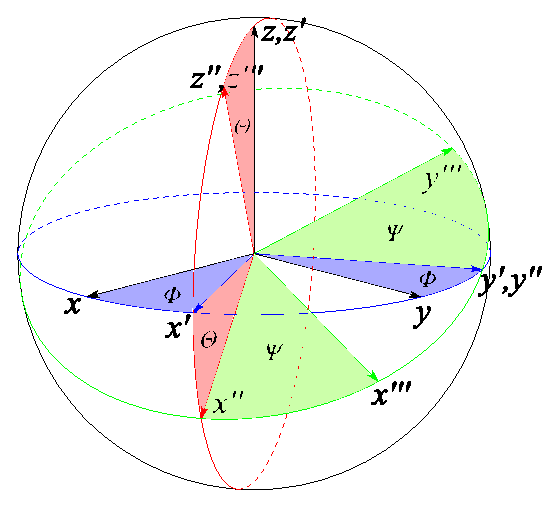
\includegraphics[scale=0.7]{_figure/euler_sphere}
\par\end{centering}

\caption [Euler angles]{The result basis vectors of the new orientation are
obtained by 3 sequential operations: (1) A rotation $\phi$ $(0<\phi<2\pi)$
about the $z$-axis, bringing the frame of axes from the initial position
S into the position ... (2) A rotation $\theta$ $(0<\theta<\pi)$
about the $y$-axis of the frame S' (3) A rotation $\psi$ $(0<\psi<2\pi)$
about the $z$-axis of the frame...\label{fig:Euler-angles}}
\end{figure}


The choice of center is often the LJ center ... ?

Pairwise additivity of intermolecular forces

The multi-body potential is often not easily dismissed, and can be taken into
account by an effective pair potential.

The effective pair potential can be measured by experiments \citep{Gray-Gubbins}
or being semi-empirical with statistical mechanical calculations.

We assume 

According to the rigid particle approximation, the pair potential
\[
\mathcal{U}(\mathbf{r}^{N},\mathbf{\Omega}^{N})=\frac{1}{2}\sum_{i\neq j}u(\mathbf{r}_{ij},\mathbf{\Omega_{i}},\mathbf{\Omega_{j}})=\sum_{i<j}u(\mathbf{r}_{ij},\mathbf{\Omega_{i}},\mathbf{\Omega_{j}})
\]


only depends on the intermolecular separation $\mathbf{r}$ and on
the molecular orientations $\mathbf{\Omega}_{1}$ and $\mathbf{\Omega}_{2}$,
\marginpar{According to the rotational invariance, $u$ can also be reduced to
$u(r,\boldsymbol{\omega_{1}},\boldsymbol{\omega_{2}})$, when $\mathbf{r}$
is referred to as polar axis.} The dependence on orientations gives properties such as...P5

This equation is quasi-exact for low density gases. The three and more
body term decreases rapidly, but it is not exact for dense fluids.

higher order corrections

\[
\mathcal{U}(\mathbf{r}^{N},\mathbf{\Omega}^{N})=\sum_{i<j}u(ij)+\sum_{i<j<k}u(ijk)+\sum_{i<j<k<l}u(ijkl)+...
\]


Three-body omission can cause surface tension problems. 
Other forces such as magnetic, multipolar, dispersion and induction
intermolecular forces are usually negligible compared to the $u_{\mu\mu}$. 

Coulomb point charge interaction

\begin{equation}
u(\mathbf{r},\mathbf{\Omega_{1}},\mathbf{\Omega_{2}})=\sum_{\alpha\beta}\frac{q_{\alpha}q_{\beta}}{r_{\alpha\beta}}
\end{equation}


Lots of models are calculated with LJ and coulomb interaction. 

site-site model

Three-body interactions


\subsection{SPC/E water and other water models}

As water is ...

There are 

The sites can placed elsewhere other than the center of atom. The more site numbers,
the more precise it becomes.

\begin{figure}[h]
\begin{centering}
\includegraphics[width=0.75\columnwidth]{_figure/water}
\par\end{centering}

\caption{Water models\label{fig:Water-models}}
\end{figure}


Model all atom

numerical density, dielectric constant vary with temperature

In this thesis, we use the extended simple point charge model (SPC/E)
of water \citep{SPC/E} as a solvent. It is a 3-site water model. The
electrostatic interaction is modeled using Coulomb's Law and the dispersion
and repulsion forces using the Lennard-Jones potential. Any similar
model possessing \textcolor{red}{...} is compatible with this theory,
as acetonitrile is used in {[}ref{]}.

The SPC/E model adds an average polarization correction to the potential
energy function:

\[
E_{\mathrm{pol}}=\frac{1}{2}\sum_{i}\dfrac{(\mu-\mu^{0})^{2}}{\alpha_{i}}
\]
where $\mu$ is the dipole of the effectively polarized water molecule
(2.35 D for the SPC/E model), $\mu^{0}$ is the dipole moment of an
isolated water molecule (1.85 D from experiment), and $\alpha_{i}$
is an isotropic polarizability constant, with a value of 1.608 \texttimes{}
10-40 F m2. Since the charges in the model are constant, this correction
just results in adding 1.25 kcal/mol (5.22 kJ/mol) to the total energy.
The SPC/E model results in a better density and diffusion constant
than the SPC model.

The SPC/E model is successful in ... 

The parameters are listed in table \ref{tab:SPC/E}, compared with
its relative SPC model.

DC \citep{Kusalik_1994_dc_spc/e}

\begin{table}
\begin{tabular}{|c|c|c|c|c|c|c|c|c|c|c|}
\hline 
 &  &  &  &  &  &  &  &  &  & \tabularnewline
\hline 
\hline 
SPC &  &  &  &  &  &  &  &  &  & \tabularnewline
\hline 
SPC/E &  &  &  &  &  &  &  &  &  & \tabularnewline
\hline 
experiment &  &  &  &  &  &  &  &  &  & \tabularnewline
\hline 
\end{tabular}

\caption{Parameters for SPC and SPC/E water\label{tab:SPC/E}}
\end{table}



\subsection{Model flexible and polarizable}

Extra degrees of freedom

interaction site can deal with non-rigidity of water

polarization

the full force field in classical

Many atoms--> expensive Long runs required to equilibrate solvent
to solute Often solvent and solute are not polarizable. Large fluctuations
due to use of small system size 


\section{Model of solute}

The model of solute also gives an influence to the energy and structure
of solvation. The compromise to have a better model of solvent or
solute is debatable, as it varies according to the application. For
example, we never use a quantum solvent model in the case of an implicit
solute since this would not be profitable even if the solute is of simple geometry
(wall). In the case of molecular solutes, we generally require the
solute to have a model at the same  or more precise scale of description
(figure \ref{fig:Hierarchy-of-models}).

\begin{flushright}
\begin{figure}[h]
\raggedleft{}%
\begin{minipage}[t]{1.1\columnwidth}%
\begin{center}
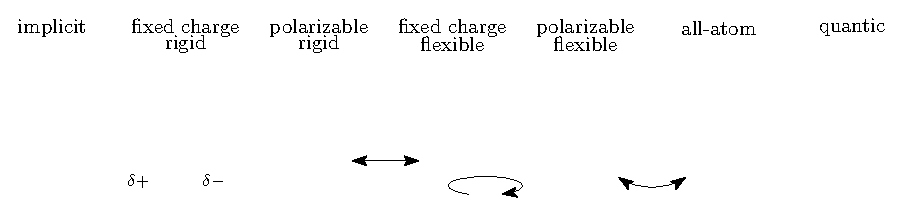
\includegraphics[width=1\columnwidth]{_figure/solute}
\par\end{center}%
\end{minipage}\caption{Hierarchy of models\label{fig:Hierarchy-of-models}}
\end{figure}

\par\end{flushright}

Most of \acs{QM} calculations in apolar solvents (toluene, etc.)
use implicit SCRF model, or even without solvent correction, and
this has proven to work well. The interaction between solute and
solvent is mainly the electrostatic interaction as described above.
Therefore 

The quantum interaction 

In this thesis, we use also rigid model to describe solute to be coherent
with IET, which cannot treat the solvent and solute in different scale
of description. 

Polarizable, flexible model, and coupling with QM is described in
perspective.



\chapter{Statistical Mechanics of Atomic Fluids\label{chpt:statistical-mechanics}}

Statistical mechanics serves to deduce thermodynamic quantities from
the Hamiltonian of any given system. In this section, we present some
basic formalism for a classical atom-like spherical solvent model
in grand canonical ensemble ($\mu$,$V$,$T$). Firstly, we introduce
the relations between the statistical mechanics and thermodynamic
quantities. Then we change the view to the structure of the solvent.
The two theories we use in this thesis, here referred to as \acs{IET}
and c\acs{DFT}, as well as their equivalency, are presented with
brief derivations in the following sections. The majority of these
sections are based on the book by Hansen \& McDonald \citep{HANSEN_2ed,Hensen-McDonald},
and the articles and notes of Evans \citep{Evans_1979,Evans_1984,Evans_1992}.
A very detailed review is done by Wu \textit{et al.} \citep{Wu2009}
to the same purpose, thus here we only introduce the concepts that
will be useful to understand this thesis.

\section{Hamiltonian and ensemble properties}

Once we define a spherical solvent model, of which the movement only
depends on its position and momentum $(\mathbf{r},\mathbf{p})$, the
instantaneous state (phase point, micro-state) of an $N$-particle
solvent system is specified by $3N$ coordinates $\mathbf{r}^{N}\equiv\mathbf{r}_{1},\ldots,\mathbf{r}_{N}$
and $3N$ momenta $\mathbf{p}^{N}\equiv\mathbf{p}_{1},\ldots,\mathbf{p}_{N}$.
The internal energy of particles in a system is characterized by its
Hamiltonian:
\begin{equation}
H_{N}(\mathbf{r}^{N},\mathbf{p}^{N})=K_{N}(\mathbf{p}^{N})+V_{N}(\mathbf{r}^{N})+V_{N}^{\mathrm{ext}}(\mathbf{r}^{N})
\end{equation}
where

\begin{tabular*}{1\columnwidth}{@{\extracolsep{\fill}}l>{\raggedright}p{0.9\columnwidth}}
$K_{N}(\mathbf{p}^{N})$ & $={\displaystyle \sum_{i=1}^{N}\frac{\mathbf{p}_{i}^{2}}{2m}}$ is
the kinetic energy;\tabularnewline
$V_{N}(\mathbf{r}^{N})$ & $={\displaystyle \sum_{i<j}^{N}u(\left|\mathbf{r}_{i}-\mathbf{r}_{j}\right|)+3\,\mathrm{body}+\ldots}$
is the interatomic potential energy $\mathcal{U}(\mathbf{r}^{N})$;\tabularnewline
$V_{N}^{\mathrm{ext}}(\mathbf{r}^{N})$ & $={\displaystyle \sum_{i=1}^{N}}V_{\mathrm{ext}}(\mathbf{r}_{i})$
is the potential energy arising from the interaction of the particles
with the external field (e.g. a solute).\tabularnewline
 & \tabularnewline
\end{tabular*}

The grand potential, characteristic thermodynamic state function for
the grand canonical ensemble, which depends on the chemical potential
$\mu$, the volume $V$ and the temperature $T$, is linked with the
statistical mechanics quantities with the relation:
\begin{equation}
\varOmega(\mu,V,T)=-k_{\mathrm{B}}T\ln\varXi\label{eq:1.2}
\end{equation}
where
\begin{eqnarray}
\varXi & = & \sum_{N=0}^{\infty}\frac{e^{\beta\mu N}}{h^{3N}N!}\int\mathrm{d}\mathbf{r}^{N}\mathrm{d}\mathbf{p}^{N}e^{-\beta H_{N}(\mathbf{r}^{N},\mathbf{p}^{N})}\\
 & = & \sum_{N=0}^{\infty}\dfrac{\text{1}}{N!}\int\mathrm{d}\mathbf{r}^{N}e^{-\beta V_{N}(\mathbf{r}^{N})}\left(\prod_{i=1}^{N}\frac{e^{\beta V_{\mathrm{int}}(\mathbf{r}_{i})}}{\Lambda^{3}}\right)
\end{eqnarray}
 is the grand partition function, with $\Lambda=\left(2\pi\beta\hbar^{2}/m\right)^{-\frac{1}{2}}$
the de Broglie thermal wavelength, and
\begin{equation}
V_{\mathrm{int}}(\mathbf{r}_{i})=\mu-V_{\mathrm{ext}}(\mathbf{r}_{i})\label{eq:1.5}
\end{equation}
the intrinsic chemical potential. 

We can also define the intrinsic free energy: \marginpar{$N=\int\mathrm{d}\mathbf{r}\bar{n}(\mathbf{r})$ is the number of
particles in canonical ensemble, but the formulae (\ref{eq:1.f-int})
and (\ref{eq:delta-f-int}) are also available for grand canonical
ensemble.}
\begin{eqnarray}
F_{\mathrm{int}} & = & F-\int\mathrm{d}\mathbf{r}\bar{n}(\mathbf{r})V_{\mathrm{ext}}(\mathbf{r})\nonumber \\
 & = & \varOmega+\mu N-\int\mathrm{d}\mathbf{r}\bar{n}(\mathbf{r})V_{\mathrm{ext}}(\mathbf{r})\nonumber \\
 & = & \varOmega+\int\mathrm{d}\mathbf{r}\bar{n}(\mathbf{r})V_{\mathrm{int}}(\mathbf{r})\label{eq:1.f-int}
\end{eqnarray}
where 
\begin{equation}
\bar{n}(\mathbf{r})=\left\langle \varrho(\mathbf{r})\right\rangle =\left\langle \sum_{i=1}^{N}\delta(\mathbf{r}-\mathbf{r}_{1})\right\rangle 
\end{equation}
is the density profile of instantaneous density $\varrho(\mathbf{r})$
distribution at equilibrium.

The differential form of $F_{\mathrm{int}}$ is
\begin{equation}
\delta F_{\mathrm{int}}=-S\delta T+\int\mathrm{d}\mathbf{r}\delta\bar{n}(\mathbf{r})V_{\mathrm{int}}(\mathbf{r})\label{eq:delta-f-int}
\end{equation}
with $S$ the entropy.

The internal energy of the solvent contains two contributions, one
due to the kinetic energy of the particles, $K_{N}(\mathbf{p}^{N})$,
and the other linked to the interaction between particles, $V_{N}(\mathbf{r}^{N})$.
When the fluid is a perfect gas, which means $V_{N}=0$, it can be
easily derived from eq. (\ref{eq:1.2}-\ref{eq:1.5}) that $F_{\mathrm{int}}$
has the following expression:
\begin{equation}
F_{\mathrm{id}}=k_{\mathrm{B}}T\int\mathrm{d}\mathbf{r}\bar{n}(\mathbf{r})\left[\ln\left(\Lambda^{3}\bar{n}(\mathbf{r})\right)-1\right]
\end{equation}
When interactions between particles are accounted for, the total expression
of $F_{\mathrm{int}}$ is:
\begin{equation}
F_{\mathrm{int}}=F_{\mathrm{id}}+F_{\mathrm{exc}}\label{eq:f-int-def}
\end{equation}
and the form of $F_{\mathrm{exc}}$ will be detailed in later sections.

\section{Functional derivatives and distribution functions}

The structure of the solvent in the grand canonical ensemble can be
characterized by its $n$-particle density 
\begin{equation}
\rho^{(n)}(\mathbf{r}^{n})=\dfrac{1}{\varXi}\sum_{N=n}^{\infty}\dfrac{1}{(N-n)!}\int\mathrm{d}\mathbf{r}^{\left(N-n\right)}e^{-\beta V_{N}(\mathbf{r}^{N})}\left(\prod_{i=1}^{N}\frac{e^{\beta V_{\mathrm{int}}(\mathbf{r}_{i})}}{\Lambda^{3}}\right)\label{eq:1.def-rho}
\end{equation}
which means the probability to find $n$ particles in a volume element
$\mathrm{d}\mathbf{r}^{n}$. In particular, the probability to find
one particle in a volume element is the solvent density $\rho^{(1)}(\mathbf{r})=\bar{n}(\mathbf{r})$,
that 
\begin{equation}
\int\rho^{(1)}(\mathbf{r})\mathrm{d}\mathbf{r}=\left\langle N\right\rangle 
\end{equation}
where $\left\langle N\right\rangle $ is the ensemble average of the
number of particles, that is to say the average number of particles
at equilibrium. $\rho^{(n)}(\mathbf{r}^{n})$ becomes $\rho^{n}$
if the system is homogeneous. It can be proven that
\begin{equation}
\dfrac{\delta\varOmega}{\delta V_{\mathrm{int}}(\mathbf{r})}=-\rho^{(1)}(\mathbf{r})
\end{equation}

The corresponding $n$-particle distribution function is defined as:
\begin{equation}
g^{(n)}(\mathbf{r}^{n})=\dfrac{\rho^{(n)}(\mathbf{r}^{n})}{\prod_{i=1}^{n}\rho^{(1)}(\mathbf{r}_{i})}
\end{equation}
such that $g^{(n)}(\mathbf{r}^{n})\rightarrow1$ when all pairs of
particles becomes sufficiently large.

The two-particle pair distribution function (\acs{PDF}), $g^{(2)}(\mathbf{r}_{1},\mathbf{r}_{2})$,
is one of the most important quantities in the theory of liquids.
Its corresponding pair correlation function (\acs{PCF}) is defined
as:
\begin{equation}
h^{(2)}(\mathbf{r}_{1},\mathbf{r}_{2})=g^{(2)}(\mathbf{r}_{1},\mathbf{r}_{2})-1
\end{equation}
which vanishes when $\left|\mathbf{r}_{1}-\mathbf{r}_{2}\right|\rightarrow\infty$.

If we define the density-density correlation function as: \marginpar{For any ensemble.}
\begin{equation}
H^{(2)}(\mathbf{r}_{1},\mathbf{r}_{2})=\rho^{(1)}(\mathbf{r}_{1})\rho^{(1)}(\mathbf{r}_{2})h^{(2)}(\mathbf{r}_{1},\mathbf{r}_{2})+\rho^{(1)}(\mathbf{r}_{1})\delta(\mathbf{r}_{1}-\mathbf{r}_{2})\label{eq:H-definition}
\end{equation}
which means the correlation \citep{Correlation_function_wiki} between
the instantaneous fluctuation of particle density from its ensemble
average, it can be proven that
\begin{equation}
\dfrac{\delta\varOmega^{2}}{\delta V_{\mathrm{int}}(\mathbf{r}_{1})\delta V_{\mathrm{int}}(\mathbf{r}_{2})}=-\beta H^{(2)}(\mathbf{r}_{1},\mathbf{r}_{2})=-\dfrac{\delta\rho^{(1)}(\mathbf{r}_{1})}{\delta V_{\mathrm{int}}(\mathbf{r}_{2})}
\end{equation}

As an analogue, the direct correlation function (\acs{DCF}) is defined
as the derivative of the excess free energy functional $F_{\mathrm{exc}}[\rho]$:

\begin{equation}
c^{(1)}(\mathbf{r})=-\dfrac{\delta(\beta F_{\mathrm{exc}}[\rho^{(1)}])}{\delta\rho^{(1)}(\mathbf{r})}
\end{equation}
\begin{equation}
c^{(2)}(\mathbf{r}_{1},\mathbf{r}_{2})=\dfrac{\delta c^{(1)}(\mathbf{r}_{1})}{\delta\rho^{(1)}(\mathbf{r}_{2})}=-\dfrac{\delta^{2}(\beta F_{\mathrm{exc}}[\rho^{(1)}])}{\delta\rho^{(1)}(\mathbf{r}_{1})\delta\rho^{(1)}(\mathbf{r}_{2})}=c^{(2)}(\mathbf{r}_{2},\mathbf{r}_{1})
\end{equation}

\begin{equation}
c^{(n)}(\mathbf{r}_{1},\ldots,\mathbf{r}_{n})=\dfrac{\delta c^{(n-1)}(\mathbf{r}_{1},\ldots,\mathbf{r}_{n-1})}{\delta\rho^{(1)}(\mathbf{r}_{n})}\label{eq:1.def-dcf}
\end{equation}

According to the definition of $F_{\mathrm{int}}$, as well as the
expression of $\delta F_{\mathrm{int}}$ in eq. (\ref{eq:delta-f-int}):
\begin{eqnarray}
\beta V_{\mathrm{int}}(\mathbf{r}) & = & \beta\dfrac{\delta F_{\mathrm{int}}[\rho^{(1)}]}{\delta\rho^{(1)}(\mathbf{r})}=\beta\dfrac{\delta F_{\mathrm{id}}[\rho^{(1)}]}{\delta\rho^{(1)}(\mathbf{r})}+\beta\dfrac{\delta F_{\mathrm{exc}}[\rho^{(1)}]}{\delta\rho^{(1)}(\mathbf{r})}\nonumber \\
 & = & \ln\left(\Lambda^{3}\rho^{(1)}(\mathbf{r})\right)-c^{(1)}(\mathbf{r})\label{eq:c1}
\end{eqnarray}

The functional derivative chain rule leads to
\begin{eqnarray}
\int\mathrm{d}\mathbf{r}_{3}\dfrac{\delta V_{\mathrm{int}}(\mathbf{r}_{1})}{\delta\rho^{(1)}(\mathbf{r}_{3})}\cdot\dfrac{\delta\rho^{(1)}(\mathbf{r}_{3})}{\delta V_{\mathrm{int}}(\mathbf{r}_{2})} & = & \int\mathrm{d}\mathbf{r}_{3}\dfrac{\delta V_{\mathrm{int}}[\rho^{(1)}(\mathbf{r}_{1})]}{\delta\rho^{(1)}(\mathbf{r}_{3})}\cdot\beta H^{(2)}(\mathbf{r}_{3},\mathbf{r}_{2})\nonumber \\
 & = & \int\mathrm{d}\mathbf{r}_{3}\left[\dfrac{1}{\rho^{(1)}(\mathbf{r}_{1})}\delta(\mathbf{r}_{1}-\mathbf{r}_{3})-c^{(2)}(\mathbf{r}_{1},\mathbf{r}_{3})\right]\cdot H^{(2)}(\mathbf{r}_{3},\mathbf{r}_{2})\nonumber \\
 & = & \delta(\mathbf{r}_{1}-\mathbf{r}_{2})
\end{eqnarray}
in addition to the definition of $H$ in eq. (\ref{eq:H-definition})
gives

\begin{equation}
h^{(2)}(\mathbf{r}_{1},\mathbf{r}_{2})=c^{(2)}(\mathbf{r}_{1},\mathbf{r}_{2})+\int\mathrm{d}\mathbf{r}_{3}\left(c^{(2)}(\mathbf{r}_{1},\mathbf{r}_{3})\rho^{(1)}(\mathbf{r}_{3})h^{(2)}(\mathbf{r}_{3},\mathbf{r}_{2})\right)\label{eq:1.oz-origine}
\end{equation}
which is called the Ornstein-Zernike (\acs{OZ}) equation. 

\section{Classical density functional theory\label{sec:Classical-density-functional}}

The density functional theory is based on two theorems :
\begin{enumerate}
\item For a given choice of $V_{N}$, $T$ and $\mu$, the intrinsic free
energy $F_{\mathrm{int}}$ is a unique functional of the equilibrium
one-particle density $\bar{n}(\mathbf{r})$, expressed by $F_{\mathrm{int}}[\bar{n}]$.
\item Let $n(\mathbf{r})$ be some arbitrary one-particle microscopic density,
and define the grand potential functional $\varOmega[n]$ as:
\begin{equation}
\varOmega[n]=F_{\mathrm{int}}[n]-\int\mathrm{d}\mathbf{r}n(\mathbf{r})V_{\mathrm{int}}(\mathbf{r})\label{eq:1.omega-p}
\end{equation}
Then the variational principle states that
\begin{equation}
\varOmega[n]\geq\varOmega[\bar{n}]
\end{equation}
with the equal sign takes at $n(\mathbf{r})=\bar{n}(\mathbf{r})$.
The differentiation of eq. (\ref{eq:1.omega-p}) with respect to $n(\mathbf{r})$
gives
\begin{equation}
\left.\frac{\delta\varOmega[n]}{\delta n(\mathbf{r})}\right|_{n=\bar{n}}=\left.\frac{\delta F_{\mathrm{int}}[n]}{\delta n(\mathbf{r})}\right|_{n=\bar{n}}-V_{\mathrm{int}}(\mathbf{r})=0\label{eq:1.26}
\end{equation}
The fact that the right hand vanishes at equilibrium is agreed with by
eq. (\ref{eq:delta-f-int}).
\end{enumerate}
The solvation free energy functional $\mathcal{F}$\marginpar{Here the character $\mathcal{F}$ is used for ``free-energy functional'';
it is a free energy of grand ensemble, but differs from Helmholtz free
energy $F$. However, it can be proven that all the free energies
become the same when the fluctuations in $N$ and $V$ are negligible
\citep{ensemble_thermo}.} is defined as the difference between the grand potential functional
of the solution system $\varOmega[n]$ and of the correspondent reference
bulk solvent at equilibrium $\varOmega[\bar{n}_{0}]$:
\begin{equation}
\mathcal{F}[n]=\varOmega[n]-\varOmega[\bar{n}_{0}]\label{eq:1.def.functional}
\end{equation}

As the external potential is absent for bulk solvent, we define:
\begin{eqnarray}
\mathcal{F}_{\mathrm{int}}[n] & = & \mathcal{F}[n]-\int\mathrm{d}\mathbf{r}n(\mathbf{r})V_{\mathrm{ext}}(\mathbf{r})\\
 & = & F_{\mathrm{int}}[n]-F_{\mathrm{int}}[\bar{n}_{0}]-\mu\int\mathrm{d}\mathbf{r}\Delta n(\mathbf{r})\nonumber \\
 & = & k_{\mathrm{B}}T\int\mathrm{d}\mathbf{r}n(\mathbf{r})\left[\ln\left(\Lambda^{3}n(\mathbf{r})\right)-1\right]+F_{\mathrm{exc}}\left[n(\mathbf{r})\right]\\
 &  & -k_{\mathrm{B}}T\int\mathrm{d}\mathbf{r}\bar{n}_{0}\left[\ln\left(\Lambda^{3}\bar{n}_{0}\right)-1\right]-F_{\mathrm{exc}}\left[\bar{n}_{0}\right]-\mu\int\mathrm{d}\mathbf{r}\Delta n(\mathbf{r})\nonumber 
\end{eqnarray}
where $\Delta n(\mathbf{r})=n(\mathbf{r})-\bar{n}_{0}$.

If we write the external free energy $F_{\mathrm{exc}}\left[n(\mathbf{r})\right]$
in Taylor expansion around $\bar{n}_{0}$:
\begin{eqnarray}
F_{\mathrm{exc}}\left[n\right] & \equiv & F_{\mathrm{exc}}\left[\bar{n}_{0}\right]+\int\mathrm{d}\mathbf{r}\left.\frac{\delta F_{\mathrm{exc}}\left[n\right]}{\delta n(\mathbf{r})}\right|_{n=\bar{n}_{0}}\Delta n(\mathbf{r})\nonumber \\
 &  & +\frac{1}{2}\int\mathrm{d}\mathbf{\mathbf{r}}_{1}\mathrm{d}\mathbf{r}_{2}\left.\frac{\delta^{2}F_{\mathrm{exc}}\left[n\right]}{\delta n(\mathbf{r}_{1})\delta n(\mathbf{r}_{2})}\right|_{n=\bar{n}_{0}}\Delta n(\mathbf{r}_{1})\Delta n(\mathbf{r}_{2})+\mathcal{O}(\Delta n^{3})\nonumber \\
 & = & F_{\mathrm{exc}}\left[\bar{n}_{0}\right]-k_{\mathrm{B}}T\int\mathrm{d}\mathbf{r}c_{0}^{(1)}(\mathbf{r})\Delta n(\mathbf{r})\nonumber \\
 &  & -\frac{k_{\mathrm{B}}T}{2}\int\mathrm{d}\mathbf{\mathbf{r}}_{1}\mathrm{d}\mathbf{r}_{2}c_{0}^{(2)}(\mathbf{r}_{1},\mathbf{r}_{2})\Delta n(\mathbf{r}_{1})\Delta n(\mathbf{r}_{2})+\mathcal{O}(\Delta n{}^{3})\label{eq:taylor-fexc}
\end{eqnarray}
where $c_{0}^{(n)}(\mathbf{r})$ is the corresponding bulk \acs{DCF}
at equilibrium defined in eq. (\ref{eq:1.def-dcf}). According to
eq. (\ref{eq:c1}):
\begin{equation}
c_{0}^{(1)}(\mathbf{r})=\ln\left(\Lambda^{3}\bar{n}_{0}\right)-\beta\mu
\end{equation}
we can find
\begin{eqnarray}
\mathcal{F}_{\mathrm{int}}[n] & = & k_{\mathrm{B}}T\int\mathrm{d}\mathbf{r}\left[n(\mathbf{r})\ln\left(\dfrac{n(\mathbf{r})}{\bar{n}_{0}}\right)-n(\mathbf{r})+\bar{n}_{0}\right]\\
 &  & -\frac{k_{\mathrm{B}}T}{2}\int\mathrm{d}\mathbf{\mathbf{r}}_{1}\mathrm{d}\mathbf{r}_{2}c_{0}^{(2)}(\mathbf{r}_{1},\mathbf{r}_{2})\Delta n(\mathbf{r}_{1})\Delta n(\mathbf{r}_{2})+\mathcal{O}(\Delta n{}^{3})\nonumber 
\end{eqnarray}

Therefore, if we define:
\begin{equation}
\mathcal{F}_{\mathrm{id}}[n]=k_{\mathrm{B}}T\int\mathrm{d}\mathbf{r}\left[n(\mathbf{r})\ln\left(\dfrac{n(\mathbf{r})}{\bar{n}_{0}}\right)-n(\mathbf{r})+\bar{n}_{0}\right]
\end{equation}
\begin{equation}
\mathcal{F}_{\mathrm{exc}}[n]=-\frac{k_{\mathrm{B}}T}{2}\int\mathrm{d}\mathbf{\mathbf{r}}_{1}\mathrm{d}\mathbf{r}_{2}c_{0}^{(2)}(\mathbf{r}_{1},\mathbf{r}_{2})\Delta n(\mathbf{r}_{1})\Delta n(\mathbf{r}_{2})+\mathcal{O}(\Delta n{}^{3})\label{eq:fexc-complet}
\end{equation}
\begin{equation}
\mathcal{F}_{\mathrm{ext}}[n]=\int\mathrm{d}\mathbf{r}n(\mathbf{r})V_{\mathrm{ext}}(\mathbf{r})
\end{equation}
the free energy functional can be written as:
\begin{equation}
\mathcal{F}[n]=\mathcal{F}_{\mathrm{int}}+\mathcal{F}_{\mathrm{ext}}=\mathcal{F}_{\mathrm{id}}+\mathcal{F}_{\mathrm{exc}}+\mathcal{F}_{\mathrm{ext}}
\end{equation}

Up to this point a brilliant approach has been built, in that for a given
choice $V_{N}$, $T$ and $\mu$, one can obtain the equilibrium density
of solvent $\bar{n}(\mathbf{r})$ by minimizing the free energy functional:
\begin{equation}
\left.\frac{\delta\mathcal{F}[n]}{\delta n(\mathbf{r})}\right|_{n=\bar{n}}=0\label{eq:1.59}
\end{equation}

Note that the two terms $\mathcal{F}_{\mathrm{id}}[n]$ and $\mathcal{F}_{\mathrm{ext}}[n]$
are physically exact, while the excess term $\mathcal{F}_{\mathrm{exc}}[n]$,
which can be rewritten as:
\begin{equation}
\mathcal{F}_{\mathrm{exc}}[n]=-\frac{k_{\mathrm{B}}T}{2}\int\mathrm{d}\mathbf{\mathbf{r}}_{1}\mathrm{d}\mathbf{r}_{2}C(\mathbf{r}_{1},\mathbf{r}_{2})\Delta n(\mathbf{r}_{1})\Delta n(\mathbf{r}_{2})
\end{equation}
depends on the exact correlation function $C(\mathbf{r}_{1},\mathbf{r}_{2})$
which is a priori unknown.

If we ignore the three-body and higher order terms in eq. (\ref{eq:fexc-complet}),
$C(\mathbf{r}_{1},\mathbf{r}_{2})$ becomes that of the homogeneous
reference fluid, which only depends on the relative distance, i.e.
$c^{(2)}(\mathbf{r}_{1},\mathbf{r}_{2})=c(r_{12})$, so that
\begin{equation}
\mathcal{F}_{\mathrm{exc}}\left[n\right]\simeq-\frac{k_{\mathrm{B}}T}{2}\int\mathrm{d}\mathbf{\mathbf{r}}_{1}\mathrm{d}\mathbf{r}_{2}c(r_{12})\Delta n(\mathbf{r}_{1})\Delta n(\mathbf{r}_{2})
\end{equation}
This was called the homogenous reference fluid (\acs{HRF}) approximation.
The generalization to a molecular, non-spherical solvent for which
orientations matter is described in $\mathsection$\ref{chpt:iem-mdft}.

\section{Integral equation theory}

Similar to the \acs{DFT} approach which aims to find the equilibrium
solvent density $\rho^{(1)}=\bar{n}$ and the free energy functional
$\mathcal{F}$, the integral equation theory (\acs{IET}) can also
give structural and energetic informations by solving a pair of integral
equations of $h^{(2)}(\mathbf{r}_{1},\mathbf{r}_{2})$ and $c^{(2)}(\mathbf{r}_{1},\mathbf{r}_{2})$
to find the pair distribution function $g$ and the difference of
correlation functions $\gamma=h-c$ which is directly linked to the
free energy. One of the relations for $h$ and $c$ is the \acs{OZ}
equation shown as eq. (\ref{eq:1.oz-origine}). Note that in $k$-space
eq. (\ref{eq:1.oz-origine}) can take advantage of the convolution
properties to give a simple product relation:
\begin{equation}
\gamma(\mathbf{k})=h(\mathbf{k})-c(\mathbf{k})=\rho\left(\gamma(\mathbf{k})+c(\mathbf{k})\right)c(\mathbf{k})\label{eq:3.oz-k}
\end{equation}

The second relation is a closure equation, which can be deduced from
eq. (\ref{eq:1.59}), giving the minimum density
\begin{equation}
\rho^{(1)}(\mathbf{r}_{1})=\rho_{0}^{(1)}\exp\left(-\beta V_{\mathrm{ext}}(\mathbf{r}_{1})+\int\mathrm{d}\mathbf{\mathbf{r}}_{2}\Delta\rho^{(1)}(\mathbf{r}_{2})c^{(2)}(\mathbf{r}_{1},\mathbf{r}_{2})+\mathcal{O}(\Delta\rho{}^{2})\right)\label{eq:1.minimize-anal}
\end{equation}
which gives, for example, when $\mathcal{O}(\Delta\rho{}^{2})=0$,
one of the simplest closure equations, the hypernetted-chain \acs{HNC}
approximation:
\begin{equation}
g(1,2)=1+h(1,2)=\exp\left[-\beta u(1,2)+h(1,2)-c(1,2)\right]
\end{equation}
Here $u$ corresponds to $V_{\mathrm{ext}}$ in eq. (\ref{eq:1.minimize-anal})
when the particles 1 and 2 are respectively the solute and solvent.

The general form of \acs{OZ} closure is:
\begin{equation}
g(1,2)=\exp\left[-\beta u(1,2)+h(1,2)-c(1,2)+b(1,2)\right]
\end{equation}
where the $b$ is the bridge function. Other closures are also possible,
such as Percus-Yevick (PY) approximation (a linear expansion of the
second exponential term in \acs{HNC}) specifically for systems with
short-range forces, or mean-spherical approximation (MSA) in the limit
of low density.

\section{Equivalence between cDFT and IET for a dilute solution system\label{sec:Equivalence-iet-mdft}}

The generalization of the \acs{OZ} equation in eq. (\ref{eq:1.oz-origine})
to $n$ components can be written as
\begin{equation}
h_{\nu\mu}(1,2)=c_{\nu\mu}(1,2)+\rho\sum_{\lambda}x_{\lambda}\int c_{\nu\lambda}(2,3)h_{\lambda\mu}(1,3)\mathrm{d}3
\end{equation}
where $x_{\nu}=N_{\nu}/N$ is the number concentration of species
$\nu\in\left[1,n\right]$.

For a two-component homogeneous solute-solvent mixture, where the
solute (M) is infinitely diluted in the solvent (S) ($x_{S}\rightarrow1$),
the coupled \acs{OZ} relations are written as
\begin{equation}
h_{\mathrm{SS}}(1,2)=c_{\mathrm{SS}}(1,2)+\rho\int h_{\mathrm{SS}}(1,3)c_{\mathrm{SS}}(2,3)\mathrm{d}3\label{eq:2oz1}
\end{equation}
\begin{equation}
h_{\mathrm{SM}}(1,2)=c_{\mathrm{SM}}(1,2)+\rho\int h_{\mathrm{SS}}(1,3)c_{\mathrm{SM}}(2,3)\mathrm{d}3\label{eq:2oz2}
\end{equation}
\begin{equation}
h_{\mathrm{MS}}(1,2)=c_{\mathrm{MS}}(1,2)+\rho\int h_{\mathrm{MS}}(1,3)c_{\mathrm{SS}}(2,3)\mathrm{d}3\label{eq:2oz3}
\end{equation}
\begin{equation}
h_{\mathrm{MM}}(1,2)=c_{\mathrm{MM}}(1,2)+\rho\int h_{\mathrm{MS}}(1,3)c_{\mathrm{SM}}(2,3)\mathrm{d}3\label{eq:2oz4}
\end{equation}

Eq. (\ref{eq:2oz1}) is the \acs{OZ} equation for bulk solvent. Eqs.
(\ref{eq:2oz2}) and (\ref{eq:2oz3}) describe the correlations between
the solute and solvents, which are equivalent. From eq. (\ref{eq:2oz3})
we can deduce eq. (\ref{eq:fexc-complet}) for the \acs{DFT} approach,
if we impose $\mathcal{O}(\Delta\rho{}^{3})=0$, i.e. the \acs{HNC}
approximation. And in \acs{IET}, eq. (\ref{eq:2oz2}) is normally
used for two-component solution. Eq. (\ref{eq:2oz4}) is rarely used.
The difficulty to solve such equation lies in finding a proper closure
equation. As the approximations like \acs{HNC} are already quantitatively
far from sufficient to describe solute-solvent correlation, it becomes
very bad for solute-solute.



\chapter{Approach to Molecular Solvents\label{chpt:iem-mdft}}

We now consider the case of a non-spherical molecular solvent, like
water. The solvent molecules now carry a molecular structure that
is described by a collection of distributed atomic interaction sites
(LJ and Coulombic). The two theories mentioned in the previous section
are formulated in the molecular picture in which each solvent molecule
is considered as a rigid body and characterized by its position, $\mathbf{r}$
(e. g. the position of center of mass), and its orientation, $\mathbf{\Omega}$,
defined by the three Euler angles $\mathbf{\Omega}\equiv(\Theta,\Phi,\Psi)$.
In \acs{MDFT}, the solvent is characterized by an inhomogeneous position
and orientation density $\rho(\mathbf{r},\mathbf{\Omega})$. In \acs{IET},
an angular dependent form of the pair distribution function $g(\mathbf{X}_{1},\mathbf{X}_{2})$
($X\equiv(\mathbf{r},\mathbf{\Omega})$) is proposed, and the molecular
\acs{OZ} equation is expanded on rotational invariants. Another way
to extend the IET is the RISM \citep{hirata_molecular_2004} which
will not be discussed in this thesis.

\section{Molecular density functional theory}

Here we can just extend some equations written in the last section
to the case of an angular-dependent external potential and density.
In \acf{MDFT}, the grand potential density functional corresponding
to an inhomogeneous fluid density $\rho(\mathbf{r},\mathbf{\Omega})$
is given by (changing notations not to confuse the traditional notation
of the grand potential with that of the orientations):
\begin{equation}
\Theta[\rho(\mathbf{r},\mathbf{\Omega})]=\Theta[\rho_{0}]+\mathcal{F}[\rho(\mathbf{r},\mathbf{\Omega})]
\end{equation}
where $\Theta[\rho_{0}]$ is the correspondent reference bulk fluid
grand potential and $\rho$ is the fluid density function depending
now on 5 or 6 variables, 3 coordinates of the positions, and 2 or
3 for the angular part depending on whether the molecule is linear or not.
The homogeneous density is equal to $n_{0}/4\pi$for a linear solvent, and
$n_{0}/8\pi^{2}$ for the general case.

According to the variation principle described above, the equilibrium
density can be found by minimizing the free energy functional $\mathcal{F}[\rho]$
regarding to $\rho(\mathbf{r},\mathbf{\Omega})$:
\begin{equation}
\left.\frac{\delta\mathcal{F}[\rho]}{\delta\rho(\mathbf{r},\mathbf{\Omega})}\right|_{\rho=\rho_{0}}=0
\end{equation}

This functional is defined as a sum of functional contributions:
\begin{equation}
\mathcal{F}[\rho]=\mathcal{F}_{\mathrm{id}}[\rho]+\mathcal{F}_{\mathrm{ext}}[\rho]+\mathcal{F}_{\mathrm{exc}}[\rho]\label{eq:fff}
\end{equation}


\subsection{The ideal term}

The ideal term $\mathcal{F}_{\mathrm{id}}[\rho]$ is deduced from
the particle interaction-free condition: 
\begin{equation}
\mathcal{F}_{\mathrm{id}}[\rho]=\beta^{-1}\int\mathrm{d}\mathbf{r}\mathrm{d\Omega}\left[\mathbf{\mathbf{\ln\left(\frac{\rho(\mathbf{r},\mathbf{\mathbf{\mathbf{\mathbf{\Omega}}}})}{\rho_{0}}\right)}}-\rho(\mathbf{r},\mathbf{\mathbf{\mathbf{\Omega}}})+\rho_{0}\right]
\end{equation}
where $\rho_{0}$ is the reference bulk density of pure solvents. The
differentiation of $\mathcal{F}_{\mathrm{id}}[\rho]$ will be used
for the minimization, discussed later, which has form
\begin{equation}
\frac{\delta\mathcal{F}_{\mathrm{id}}[\rho]}{\delta\rho(\mathbf{r},\mathbf{\Omega})}=\beta^{-1}\ln\left(\dfrac{\rho(\mathbf{r},\mathbf{\Omega})}{\rho_{0}}\right)
\end{equation}


\subsection{The external term}

The solute, like the solvent, is described in microscopic detail by
a molecular non-polarizable force field involving atomic Lennard-Jones
and partial charge parameters, creating at each point in space an
external potential ($V_{\mathrm{ext}}(\mathbf{r},\mathbf{\mathbf{\mathbf{\mathbf{\Omega}}}})$),
containing two components:
\begin{equation}
V_{\mathrm{ext}}(\mathbf{r},\mathbf{\Omega})=V_{\mathrm{LJ}}(\mathbf{r})+V_{\mathrm{coul}}(\mathbf{r},\mathbf{\Omega})
\end{equation}

The external potential term calculates the contribution of $V_{\mathrm{ext}}$:
\begin{equation}
\mathcal{F}_{\mathrm{ext}}[\rho]=\int\mathrm{d}\mathbf{r}\mathrm{d}\mathbf{\mathbf{\Omega}}V_{\mathrm{ext}}(\mathbf{r},\mathbf{\mathbf{\mathbf{\mathbf{\Omega}}}})\rho(\mathbf{r},\mathbf{\mathbf{\mathbf{\mathbf{\Omega}}}})
\end{equation}

The Lennard-Jones potential is given by
\begin{equation}
V_{\mathrm{LJ}}(\mathbf{r})=\sum_{u}\sum_{v}4\epsilon_{uv}\left[\left(\dfrac{\sigma_{uv}}{r_{uv}}\right)^{12}-\left(\dfrac{\sigma_{uv}}{r_{uv}}\right)^{6}\right]\label{eq:LJ}
\end{equation}

where $u$ stands for solute, $v$ stands for solvent, $\epsilon_{uv}=\sqrt{\epsilon_{u}\epsilon_{v}}$
and $\sigma_{uv}=\left(\sigma_{u}+\sigma_{v}\right)$ are the geometric
and arithmetic average Lennard-Jones parameters between solute and
solvent, according to the Lorentz-Berthelot mixing rules. $r_{ij}$
is the norm of relative site-site vector
\begin{equation}
\mathbf{r}_{uv}=\mathbf{r}+\mathbf{R}(\mathbf{\Omega})\mathbf{s}_{v}-\mathbf{r}_{u}\label{eq:ruv}
\end{equation}
where $\mathbf{r}_{u}$ and $\mathbf{s}_{j}$ are the coordinates
of solute/solvent molecules in the molecular frame, and $\mathbf{R}(\mathbf{\Omega})$
is the rotation matrix of the Euler angles $\mathbf{\Omega}$.

In cases where the solvent site wears only one LJ centre, eq. (\ref{eq:ruv})
reduces to

\begin{equation}
\mathbf{r}_{uv}=\mathbf{r}-\mathbf{r}_{u}
\end{equation}
which is actually what we use in the code as the solvent is SPC/E
water.

The Coulomb interaction is calculated by \textcolor{red}{solving the
Poisson equation \citep{Marchi_2001}.} The charge density of the
solute is projected onto a space grid,
\begin{equation}
\rho_{q}(\mathbf{r})=\sum_{u}q_{ijk}
\end{equation}
where $q_{ijk}$ is the charge on the space grid distributed by its
nearby point charge as shown in figure \ref{fig:Charge-density-projected}
(a).

\begin{figure}[h]
\begin{centering}
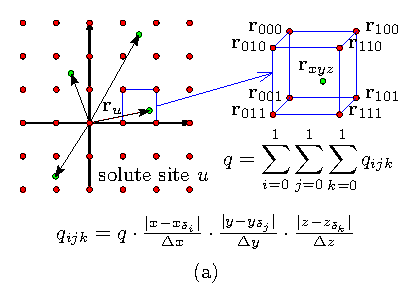
\includegraphics{_figure/charge_int}
\par\end{centering}
\caption{Charge density projected onto grids\label{fig:Charge-density-projected}.
(a) Solute. (b) Solvent.}
\end{figure}

\begin{equation}
V_{\mathrm{coul}}(\mathbf{r},\mathbf{\Omega})=\sum_{v}q_{v}V_{q}(\mathbf{r}_{u})
\end{equation}
where $V_{q}(\mathbf{r})$ is the electrostatic potential created
by the charge distribution $\rho_{q}(\mathbf{r})$. It can be computed
using a periodic Poisson Solver. The Poisson equation reads

\begin{equation}
\nabla^{2}V_{q}(\mathbf{r})=-\frac{\rho_{q}(\mathbf{r})}{\varepsilon_{0}}
\end{equation}

or in Fourier space
\begin{equation}
\hat{V}_{q}(\mathbf{k})=\frac{\hat{\rho}_{q}(\mathbf{k})}{\varepsilon_{0}k^{2}}
\end{equation}
where $\hat{V}_{q}(\mathbf{k})$, $\hat{\rho}_{q}(\mathbf{k})$ are
the Fourier transform of $V_{q}(\mathbf{r})$, $\rho_{q}(\mathbf{r})$
respectively. $\rho_{q}(\mathbf{r})$ is transformed forward, $\hat{V}_{q}(\mathbf{k})$
is computed and transformed backward. $V_{q}(\mathbf{r}_{u})$ is
then obtained by interpolation. 

\subsection{The excess term}

The two terms $\mathcal{F}_{\mathrm{id}}[\rho]$ and $\mathcal{F}_{\mathrm{ext}}[\rho]$
are physically exact, while the excess term $\mathcal{F}_{\mathrm{exc}}[\rho]$
depends on the exact correlation function, which is a priori unknown.
As in the previous section, we invoke here the \acs{HRF} approximation
which amounts to a second-order Taylor expansion around the homogeneous
fluid at density $\rho_{0}$:
\begin{equation}
\mathcal{F}_{\mathrm{exc}}[\rho]=\frac{k_{B}T}{2}\int\mathrm{d}\mathbf{r_{1}}\mathrm{d}\mathbf{\mathbf{\Omega}}\gamma(\mathbf{r}_{1},\mathbf{\mathbf{\mathbf{\mathbf{\Omega}}}})\rho(\mathbf{r_{1}},\mathbf{\mathbf{\mathbf{\mathbf{\Omega}}}})\label{eq:fexc}
\end{equation}
where $\gamma$ is the normalized gradient of the excess functional:
\begin{equation}
\gamma(\mathbf{r_{1}},\mathbf{\Omega_{1}})=\frac{\delta\beta F_{\mathrm{exc}}}{\delta\rho}=-\int\mathrm{d}\mathbf{r_{2}}\mathrm{d}\mathbf{\Omega_{2}}\Delta\rho(\mathbf{r}_{2},\mathbf{\Omega}_{2})c(\mathbf{r}_{12},\mathbf{\Omega}_{1},\mathbf{\Omega}_{2})\label{eq:gamma}
\end{equation}

To evaluate the gradient $\gamma$ for each $\mathbf{(r},\mathbf{\Omega})$,
$N\equiv N_{\mathbf{r}}N_{\mathbf{\Omega}}$ function evaluations
(\acs{FE}) are required. The total number of \acs{FE} is thus $N^{2}=O(N^{2})$,
which, with typically $N_{\mathbf{r}}=64^{3}$ and $N_{\mathbf{\Omega}}=50\sim100$,
is far too costly for current computing technology. For this reason,
Fourier transform is used to treat the spatial convolution in eq.
(\ref{eq:gamma}).

A convolution
\begin{equation}
h(x_{1})\equiv f(x_{2})\otimes g(x_{2})\equiv\int_{a}^{b}f(x_{2})g(x_{1}-x_{2})dx_{2}\label{eq:convolution-1}
\end{equation}
has the property that
\begin{equation}
\mathfrak{F}[h(x_{1})]=\mathfrak{F}[f(x_{2})]\mathfrak{F}[g(x_{2})]\label{eq:convolution-2}
\end{equation}
$\mathfrak{F}$ being the Fourier transform operation. As $\mathbf{r_{12}}=\mathbf{r_{1}}-\mathbf{r_{2}}$,
eq. (\ref{eq:gamma}) is a 3D convolution, which leads to
\begin{equation}
\hat{\gamma}(\mathbf{k},\mathbf{\Omega_{1}})=-\beta^{-1}\int\mathrm{d}\mathbf{\Omega}_{2}\Delta\hat{\rho}(\mathbf{k},\mathbf{\Omega}_{2})\hat{c}(\mathbf{k},\mathbf{\Omega}_{1},\mathbf{\Omega}_{2})\label{eq:gamma-k}
\end{equation}

Thus the integral $\int\mathrm{d}\mathbf{r_{2}}$ in eq. (\ref{eq:gamma})
is transformed into a simple product in eq. (\ref{eq:gamma-k}). To
get $\hat{\gamma}(\mathbf{k},\mathbf{\Omega_{1}})$ with given $\Delta\hat{\rho}(\mathbf{k},\mathbf{\Omega_{2}})$,
only $N_{\mathbf{r}}N_{\mathbf{\Omega}}^{2}$\acs{FE} are needed.
To this computational cost should be added the transform from $\Delta\rho(\mathbf{r},\mathbf{\Omega})$
to $\Delta\hat{\rho}(\mathbf{k},\mathbf{\Omega})$ and the backward
transform from $\hat{\gamma}(\mathbf{k},\mathbf{\Omega})$ to $\gamma(\mathbf{r},\mathbf{\Omega})$
which are both of order $N_{\mathbf{\Omega}}\cdot O(N_{\mathbf{r}}\log_{2}N_{\mathbf{r}})$
due to the properties of Fast Fourier Transforms (\acs{FFT}). The
total number of \acs{FE} is thus reduced from quadratic complexity
$O(N_{\mathbf{r}}^{2}N_{\mathbf{\Omega}}^{2})$ to $N_{\mathbf{r}}N_{\mathbf{\Omega}}^{2}+2N_{\mathbf{\Omega}}\cdot O(N_{\mathbf{r}}\log_{2}N_{\mathbf{r}})=O(N_{\mathbf{r}}\log_{2}N_{\mathbf{r}}N_{\mathbf{\Omega}}^{2})$.
As the total number of spatial grid $N_{\mathbf{r}}$ is of magnitude
$10^{5}\sim10^{6}$, this procedure, which is mathematically equivalent
to the direct evaluation (\ref{eq:gamma}), offers a great advantage
in terms of computational efficiency (figure \ref{fig:order-of-growth}
in section \ref{chpt:introduction}).

Once $\gamma(\mathbf{r},\mathbf{\Omega})$ is obtained by inverse
Fourier transform of $\gamma(\mathbf{r},\mathbf{\Omega})$, the excess
functional can be calculated as eq. (\ref{eq:fexc}).

The input $\hat{c}(\mathbf{k},\mathbf{\Omega}_{1},\mathbf{\Omega}_{2})$
is an angular-dependent \acs{DCF} of the homogeneous solvent which
depends on the relative position of two molecules $r_{12}$ and their
orientations (two in the initial code \citep{Zhao_2011}, and three
developed in this thesis). This quantity is provided with high
precision and in different representations by Luc Belloni, using a
mixture of Monte-Carlo simulations and inversion of the angular-dependent
\acs{MOZ} equation within a rotational invariant expansion \citep{puibasset_bridge_2012}.
A detailed comparison of some \acs{DCF}s is in appendix \textcolor{red}{{[}ref{]}}.

\section{Angular dependent integral equation theory}

To extend the \acs{IET} formalism to molecular cases, Blum \citep{Blum_I,Blum_II}
proposed an angular-dependent form of the pair distribution function,
which is then used in the \acs{IET} formalism. Fries \& Patey \citep{Fries_Patey_1985}
proposed the numerical solution of the full \acs{HNC} theory using
angle-dependent pair potentials. The description below is based on
these articles.

The angular-dependent \acs{PDF} is defined as 
\begin{equation}
g(\mathbf{X}_{1},\mathbf{X}_{2})\equiv g(\mathbf{r}_{1},\mathbf{r}_{2},\mathbf{\Omega}_{1},\mathbf{\Omega}_{2})
\end{equation}
which possesses the translational invariance if the fluid is homogeneous:
\begin{equation}
g(\mathbf{X}_{1},\mathbf{X}_{2})=g(\mathbf{r}_{12},\mathbf{\Omega}_{1},\mathbf{\Omega}_{2})
\end{equation}
and the rotational invariance \textcolor{red}{(attention indices)}:
\begin{equation}
g(\mathbf{X}_{1},\mathbf{X}_{2})=\sum_{m,n,l=0}^{\infty}\sum_{\left|\mu,\mu'\right|\leq m,\left|\nu,\nu'\right|\leq m,\left|\lambda\right|\leq l}g_{\mu,\mu'\nu\nu'\lambda}^{mnl}(\left\Vert \mathbf{r}_{12}\right\Vert )R_{\mu\mu'}^{m}(\mathbf{\Omega}_{1})R_{\nu\nu'}^{m}(\mathbf{\Omega}_{2})R_{\lambda0}^{l}(\hat{\mathbf{r}}_{12})
\end{equation}

The suggestion of Wigner gives a set of rotation invariant:
\begin{equation}
\Phi_{\mu'\nu'}^{mnl}(\hat{\mathbf{r}}_{12},\mathbf{\Omega}_{1},\mathbf{\Omega}_{2})=f^{mnl}\sum_{\mu\nu\lambda}\left(\begin{array}{ccc}
m & n & l\\
\mu & \nu & \lambda
\end{array}\right)R_{\mu\mu'}^{m}(\mathbf{\Omega}_{1})R_{\nu\nu'}^{m}(\mathbf{\Omega}_{2})R_{\lambda0}^{l}(\hat{\mathbf{r}}_{12})
\end{equation}
such that
\begin{equation}
g(\mathbf{X}_{1},\mathbf{X}_{2})=\sum_{mnl}\sum_{\mu'\nu'}g_{\mu'\nu'}^{mnl}(\left\Vert \mathbf{r}_{12}\right\Vert )\Phi_{\mu'\nu'}^{mnl}(\hat{\mathbf{r}}_{12},\mathbf{\Omega}_{1},\mathbf{\Omega}_{2})
\end{equation}
and
\begin{equation}
g_{\mu'\nu'}^{mnl}=\sum_{\mu\nu\lambda}\left(\begin{array}{ccc}
m & n & l\\
\mu & \nu & \lambda
\end{array}\right)g_{\mu,\mu'\nu\nu'\lambda}^{mnl}
\end{equation}

The molecular Ornstein-Zernike \acs{MOZ} equation is defined as
\begin{equation}
h(\mathbf{X}_{1},\mathbf{X}_{2})-c(\mathbf{X}_{1},\mathbf{X}_{2})=\frac{\rho}{8\pi^{2}}\int\mathrm{d}\mathbf{X}_{3}h(\mathbf{X}_{1},\mathbf{X}_{3})c(\mathbf{X}_{3},\mathbf{X}_{2})
\end{equation}
which can be both expanded as
\begin{equation}
h(\mathbf{X}_{1},\mathbf{X}_{2})=\sum_{mnl}\sum_{\mu'\nu'}h_{\mu'\nu'}^{mnl}(\left\Vert \mathbf{r}_{12}\right\Vert )\Phi_{\mu'\nu'}^{mnl}(\hat{\mathbf{r}}_{12},\mathbf{\Omega}_{1},\mathbf{\Omega}_{2})
\end{equation}
\begin{equation}
c(\mathbf{X}_{1},\mathbf{X}_{2})=\sum_{mnl}\sum_{\mu'\nu'}c_{\mu'\nu'}^{mnl}(\left\Vert \mathbf{r}_{12}\right\Vert )\Phi_{\mu'\nu'}^{mnl}(\hat{\mathbf{r}}_{12},\mathbf{\Omega}_{1},\mathbf{\Omega}_{2})
\end{equation}
\begin{equation}
\eta(\mathbf{X}_{1},\mathbf{X}_{2})=h(\mathbf{X}_{1},\mathbf{X}_{2})-c(\mathbf{X}_{1},\mathbf{X}_{2})=\sum_{mnl}\sum_{\mu'\nu'}\eta_{\mu'\nu'}^{mnl}(\left\Vert \mathbf{r}_{12}\right\Vert )\Phi_{\mu'\nu'}^{mnl}(\hat{\mathbf{r}}_{12},\mathbf{\Omega}_{1},\mathbf{\Omega}_{2})
\end{equation}
As an analog to the \acs{FFT} the fast Hankel transform can deal
these rotational invariant projections into $k$-space, such that
\begin{equation}
\hat{c}_{\mu\nu}^{mnl}(k)=4\pi i^{l}\int\mathrm{d}r\,r^{2}j_{l}(kr)c_{\mu\nu}^{mnl}(r)
\end{equation}
\begin{equation}
\hat{\eta}_{\mu\nu}^{mnl}(k)=4\pi i^{l}\int\mathrm{d}r\,r^{2}j_{l}(kr)\eta_{\mu\nu}^{mnl}(r)
\end{equation}
where $j_{l}(kr)$ are the spherical Bessel functions.

The $\chi$-transform defined by Blum gives
\begin{equation}
\hat{c'}_{\mu\nu,\chi}^{mn}(k)=\sum_{l=\left|m-n\right|}^{m+n}\left(\begin{array}{ccc}
m & n & l\\
\chi & -\chi & 0
\end{array}\right)\hat{c}_{\mu\nu}^{mnl}(k)
\end{equation}
\begin{equation}
\hat{\eta'}_{\mu\nu,\chi}^{mn}(k)=\sum_{l=\left|m-n\right|}^{m+n}\left(\begin{array}{ccc}
m & n & l\\
\chi & -\chi & 0
\end{array}\right)\hat{\eta}_{\mu\nu}^{mnl}(k)
\end{equation}
If $\Phi_{\mu'\nu'}^{mnl}(\hat{\mathbf{r}}_{12},\mathbf{\Omega}_{1},\mathbf{\Omega}_{2})$
is defined with the factor $f^{mnl}=\left[(2m+1)(2n+1)\right]^{1/2},$
the \acs{MOZ} equation can be reduced by Blum's reduction such that
\begin{equation}
\hat{\eta'}_{\mu\nu,\chi}^{mn}(k)=\rho\sum_{n_{1}}\sum_{\nu_{1}=-n_{1}}^{n_{1}}(-)^{\chi+\nu_{1}}\left[\hat{\eta'}_{\mu\nu_{1},\chi}^{mn_{1}}(k)+\hat{c'}_{\mu\nu_{1},\chi}^{mn_{1}}(k)\right]\hat{c'}_{\underline{\nu_{1}}\nu,\chi}^{n_{1}n}(k)
\end{equation}
which reduces the calculation of $(\mathbf{X}_{1},\mathbf{X}_{3})$
for $(\mathbf{X}_{3},\mathbf{X}_{2})$ to a sum of $n_{1}$, $\nu_{1}$.

\textcolor{red}{(The part of HNC has non need in this thesis.)}



\chapter{Code MDFT\label{chpt:mdft}}

The code MDFT upon which all the development in this thesis is
based is a Fortran 95 sequential code developed by Maximilien Levesque,
Daniel Borgis \textit{et al.} \citep{gendre_classical_2009,jeanmairet_molecular_2013-1,jeanmairet_molecular_2015,jeanmairet_molecular_2016,Jeanmairet_thesis,levesque_solvation_2012,ramirez_density_2002,ramirez_density_2005,sergiievskyi_fast_2014,Zhao_2011},
which implements the \acs{MDFT} theory. It reads the force field (Lennard-Jones
and Coulomb parameters) describing the solute and the solvent as input,
as well as necessary parameters like the temperature $T$, number
density of solvent $n_{0}$, etc. It minimizes the functional and
gives the equilibrium density $\rho(\mathbf{r},\mathbf{\Omega})$,
then computes output properties.

\section{Supercell discretization}

$L_{x}\times L_{y}\times L_{z}$ $\left[\textrm{Å}^{3}\right]$ space
is discretized on a regular grid of $\textrm{nfft}_{1}\times\textrm{nfft}_{2}\times\textrm{nfft}_{3}$
nodes. The solute center is at $\mathbf{r}_{T}=\left(\dfrac{L_{x}}{2},\dfrac{L_{y}}{2},\dfrac{L_{z}}{2}\right)$
of the box. If the internal coordinates of solute $\mathbf{r}_{M}$,
the solute coordinates in the box $\mathbf{r}=\mathbf{r}_{M}+\mathbf{r}_{T}$.

Angular grid is discretized with Lebedev (L) quadrature for $\mathbf{\Omega}\equiv\left(\Theta,\Phi\right)$,
$\Theta\in\left[0,\pi\right]$, $\Phi\in\left[0,2\pi\right]$, or
Gauss-Legendre (GL) quadrature for $\Theta$ and trapezoidal quadrature
for $\Phi$. $\Psi\in\left[0,\pi\right]$ as we used the code mainly
for water, is discretized with trapezoidal quadrature. The number
of each angular dimension is linked to the order of quadrature, $m_{\max}$,
which is discussed mainly in the chapter of theory.

\section{Minimizer L-BFGS-B}

The minimizer adopted by \acs{MDFT} is the L-BFGS-B \citep{Zhu_1994_bfgs,Zhu_bfgs_1997_algorithm}
package version 3.0 written in Fortran 77, implementing the limited-memory
Broyden-Fletcher-Goldfarb-Shanno (BFGS) algorithm with constraints
of the form $l\leq x\leq u$ to the variable $x$.

The functional $\mathcal{F}[x_{i}]$ and the gradient of functional
$\nabla\mathcal{F}[x_{i}]=\dfrac{\delta\mathcal{F}}{\delta x}(x_{i})$
are required by L-BFGS to minimize the functional. It saves the variables
$x_{i}$ and gradients of the past $m$ iterations, which requires
a lot of memory.

The functional in MDFT to be minimized is eq. (\ref{eq:4.fff}):
\begin{equation}
\mathcal{F}[\rho]=\mathcal{F}_{\mathrm{id}}[\rho]+\mathcal{F}_{\mathrm{ext}}[\rho]+\mathcal{F}_{\mathrm{exc}}[\rho]
\end{equation}
and its gradient is
\begin{equation}
\frac{\delta\mathcal{F}[\rho]}{\delta\rho(\mathbf{r},\mathbf{\Omega})}=k_{\mathrm{B}}T\ln\left(\dfrac{\rho(\mathbf{r},\mathbf{\Omega})}{\rho_{0}}\right)+V_{\mathrm{exc}}(\mathbf{r},\mathbf{\Omega})+V_{\mathrm{ext}}(\mathbf{r},\mathbf{\Omega})
\end{equation}
where $\rho_{0}$ is the angular density of bulk solvent, 
\begin{equation}
\rho_{0}=\left\{ \begin{array}{ll}
n_{0} & \mbox{if atomic, }\Omega\equiv1\\
n_{0}/4\pi & \mbox{if linear, }\Omega\equiv(\Theta,\Phi)\\
n_{0}/8\pi^{2} & \mbox{if non-linear, }\Omega\equiv(\Theta,\Phi,\Psi)
\end{array}\right.\label{eq:rho}
\end{equation}
such that $\int\mathrm{d}\mathbf{\Omega}\rho(\mathbf{r},\mathbf{\Omega})/\rho_{0}=n(\mathbf{r})/n_{0}$
is normalized to 1 when $r\rightarrow\infty$.

\section{Treatment to avoid unphysical density}

During minimization, the density variable $\rho(\mathbf{r},\mathbf{\Omega})$
can have unphysical negative numbers, which also cause the divergence
of the minimization. To avoid this phenomenon, a normalized $\varphi(\mathbf{r},\mathbf{\Omega})$
is used as the variable during the minimization in place of $\rho(\mathbf{r},\mathbf{\Omega})$,
so that:
\begin{equation}
\rho(\mathbf{r},\mathbf{\Omega})=\rho_{0}\varphi^{2}(\mathbf{r},\mathbf{\Omega})\label{eq:cg_vect}
\end{equation}

According to the definition (\ref{eq:cg_vect}), we see:
\begin{equation}
\frac{\delta\rho(\mathbf{r},\mathbf{\Omega})}{\delta\varphi}=2\rho_{0}\varphi(\mathbf{r},\mathbf{\Omega})
\end{equation}

Therefore the gradient to feed the L-BFGS minimizer is:
\begin{equation}
\frac{\delta\mathcal{F}}{\delta\varphi}=\frac{\delta\mathcal{F}}{\delta\rho}\cdot\frac{\delta\rho}{\delta\varphi}=2\rho_{0}\varphi(\mathbf{r},\mathbf{\Omega})\cdot\left[\beta^{-1}\ln\varphi^{2}+V_{\mathrm{exc}}+V_{\mathrm{ext}}\right]
\end{equation}

The main structure of the code is shown in figure \ref{fig:code-mdft}.
\begin{figure}[H]
\begin{centering}
\includegraphics[width=1\columnwidth]{_figure/mdft}
\par\end{centering}
\caption{Main structure of code MDFT\label{fig:code-mdft}}
\end{figure}


\section{Fast Fourier transform}

The fast Fourier transform (\acs{FFT}) is used in the
evaluation of excess functional in eq. (\ref{eq:4.gamma-k}); in this
thesis, the FFTW3 library \citep{FFTW3} is used for implementation,
which performs discrete Fourier Transform (\acs{DFT}) as defined
below:
\begin{equation}
Y_{k}=\sum_{j=0}^{n-1}X_{j}e^{-2\pi ijk/n}\begin{array}{c}
\mathrm{(forward)}\end{array}\label{eq:fftw3-fwd}
\end{equation}
\begin{equation}
X_{j}=\sum_{k=0}^{n-1}Y_{k}e^{2\pi ijk/n}\begin{array}{c}
\mathrm{(backward)}\end{array}\label{eq:fftw3-bwd}
\end{equation}

Note that after a forward-backward Fourier transform, the original
function is multiplied by a normalization factor $N_{k}$, which is
the total number of nodes $k$.

For input function $Y_{k}$ $(k=0,\ldots,n-1)$ in real numbers, FFTW3
only outputs elements $k=0,\ldots,\left\lfloor n/2\right\rfloor $
( $\left\lfloor n/2\right\rfloor +1$ complex numbers of $X_{j}$
are stocked; $\left\lfloor n/2\right\rfloor $ being the floor function
of $n/2$), with the “Hermitian” symmetry
\begin{equation}
Y_{k}=Y_{n-k}^{*}\label{eq:yk_conjg}
\end{equation}
used to regenerate elements of $k>\left\lfloor n/2\right\rfloor $.
The resulting $X_{j}$ issued from the corresponding backward transform
is purely real. 

The definition of \acs{FFT} can differ in some literature, with
the ``$+$'' sign in the exponential of forward transform and ``$-$''
sign in the exponential of backward transform. According to the Hermitian
symmetry, we should use the quantities in $k$-space issued from such
a definition with its conjugate form.


\ctparttext{This chapter presents a complete theory of the $\mathcal{F}_{\mathrm{exc}}$
evaluation under HRF approximation: 
\[
\mathcal{F}_{\mathrm{exc}}=-\frac{\beta^{-1}}{2}\int\mathrm{d}\mathbf{r_{1}}\mathrm{d}\mathbf{r_{2}}\mathrm{d}\mathbf{\Omega_{1}}\mathrm{d}\mathbf{\Omega_{2}}\Delta\rho(\mathbf{r_{1}},\mathbf{\Omega_{1}})\Delta\rho(\mathbf{r_{2}},\mathbf{\Omega_{2}})c(r_{12},\mathbf{\Omega_{1}},\mathbf{\Omega_{2}})
\]
which is based on previous work of Zhao et al. \citep{Zhao_2011},
where the HRF approximation bas been applied to linear molecules ($\mathbf{\Omega}\equiv(\Theta,\Phi)$).
In this thesis, the method is generated to molecular solvent, using
3 Euler angles, i. e. $\mathbf{\Omega}\equiv(\Theta,\Phi,\Psi)$,
where the computing cost of the original algorithm is no longer reasonable.
Further approximation is therefore made, where the density variable
$\rho(\mathbf{r},\mathbf{\Omega})$ is expended on generalized spherical
harmonics. Theoretically, this approximation gives little loss of
accuracy, but makes a great advantage in computing time and memory
requirement. The prove is shown in the implementation part.\\
\medskip{}
Section \ref{chpt:fft-spatial} describes the FFT treatment for the
spatial convolution in the gradient $\gamma$ of the excess functional
$\mathcal{F}_{\mathrm{exc}}$, which reduces the algorithm complexity
from $O(N^{2})$ to $O(N\log_{2}N)$. A DCF directly issue of Monte
Carlo simulation and solution HNC is used, in both intermolecular
and projection form. To use the intermolecular form, the matrix which
does the transform from laboratory to intermolecular coordinates system
is generalized to molecular case compared to previous work, then interpolation
of zero and first order is involved. To use the projection from, DCF
is reconstructed with all projections. For order of projections $n_{\mathrm{max}}=1$,
the formula of each projections are written explicitly. \\
\medskip{}
Section \ref{chpt:angular-convolution} presents the treatment of
angular convolution. As IEM and MDFT have mathematical equivalence,
an algorithm inspired by the work of Fries \citep{Fries_Patey_1985}
and Blum \citep{Blum_I,Blum_II} for IEM is built for MDFT. In this
algorithm, the density variable $\rho(\mathbf{r},\mathbf{\Omega})$
is expended on generalized spherical harmonics, then rotated onto
intermolecular frame. It is shown that in this form, the OZ equation
is largely simplified.\\
\medskip{}
The solvent properties involved in this thesis are presented in the
next two chapters. Section \ref{chpt:thermodynamic-quantities} presents
some thermodynamic quantities, including the solvation free energy
and its corrections, ... and section \ref{chpt:solvation-structure}
gives some forms of structure that can be preformed, such as the radical
distribution function, radical polarization functions, rotational
invariants expansion, etc.}

\part{Theory: HRF Approximation, For Molecular Solvent}


\chapter{Angular Integration in Excess Functional \label{chpt:fft-spatial}}

As discussed in last chapter, the Fourier transform of the excess
functional gradient is:
\begin{equation}
\hat{\gamma}(\mathbf{k},\mathbf{\Omega}_{1})=\int\mathrm{d}\mathbf{\Omega}_{2}\Delta\hat{\rho}(\mathbf{k},\mathbf{\Omega}_{2})\hat{c}(\mathbf{k},\mathbf{\Omega}_{1},\mathbf{\Omega}_{2})\label{eq:gamma-k}
\end{equation}

It should be pointed out that the direct correlation function (\acs{DCF}),
$\hat{c}(\mathbf{k},\mathbf{\Omega}_{1},\mathbf{\Omega}_{2})$, used
as an input data in eq. (\ref{eq:gamma-k}) is very memory-costly.
In the previous work \citep{gendre_classical_2009,Zhao_2011,borgis_molecular_2012},
the \acs{DCF} bas been stocked in the intermolecular form $\hat{c}(k,\boldsymbol{\omega}_{1},\boldsymbol{\omega}_{2})$
to profit an economy of memory, where $(\boldsymbol{\omega}_{1},\boldsymbol{\omega}_{2})\equiv(\cos\theta_{1},\cos\theta_{2},\phi_{12})$,
and the correspondence of $(\mathbf{\Omega}_{1},\mathbf{\Omega}_{2})$
to $(\boldsymbol{\omega}_{1},\boldsymbol{\omega}_{2})$ is calculated
directly in the code. These works adapt well with linear solvents,
but are proved less powerful for molecular solvent such as water.
However, in the case of full Euler angles intermolecular \acs{DCF}
(fig. \ref{fig:coordinate_systems}), 
\begin{equation}
\hat{c}(k,\boldsymbol{\omega}_{1},\boldsymbol{\omega}_{2})\equiv\hat{c}(k,\cos\theta_{1},\cos\theta_{2},\phi,\psi_{1},\psi_{2})
\end{equation}
neither the storage of $\hat{c}(\mathbf{k},\mathbf{\Omega}_{1},\mathbf{\Omega}_{2})$
which is definitively impossible, nor the direct calculation of correspondence
$(\mathbf{\Omega}_{1},\mathbf{\Omega}_{2})$ to $(\boldsymbol{\omega}_{1},\boldsymbol{\omega}_{2})$
due to the increased complexity that makes it too costly, can be regard
as a possible solution. For instance, with a normal setting of $64^{3}$
spatial grid and a Lebedev quadrature of order 2 (14 angles for $\Theta$
and $\Phi$), and 3 $\Psi$-angles, even if the \acs{DCF} is stocked
in simple precision (complex number), it takes $64^{3}\times42^{2}\times4\,\mathrm{bytes}\times2=3.52\mathrm{GB}$,
and for a Lebedev quadrature of order 5 and correspondingly 5 $\Psi$-angles,
it takes $64^{3}\times250^{2}\times4\,\mathrm{bytes}\times2=131\mathrm{GB}$.
As a normal PC has only 4 to 16 GB of RAM, it can cause a memory leak. 

Therefore, two strategies are developed to treat the full \acs{DCF}
case. The first one is a direct extension of the previous work, which
uses the full intermolecular \acs{DCF} with a more complicate angle
correspondence pre-tabulated in the beginning of the implementation.
The other calculates the \acs{DCF} directly from rotational invariant
projections. Here we give a complete discussion of these two strategies.

\begin{figure}[H]
\begin{centering}
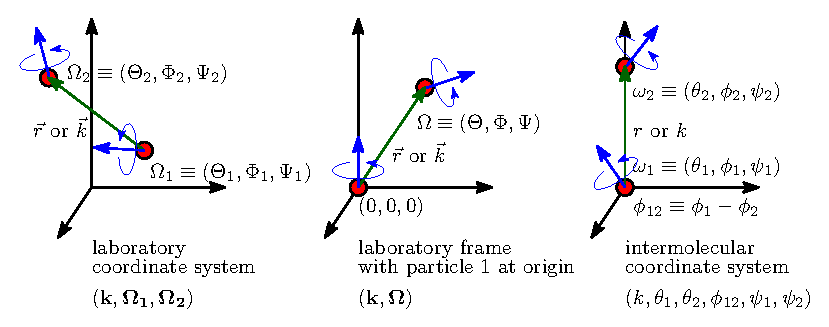
\includegraphics{_figure/coordinate_system}
\par\end{centering}
\caption[Molecules 1 and 2 in different coordinate systems]{Molecules 1 and 2 in different coordinate systems. The laboratory
coordinate system is the system of our grid with a fixed reference
view. When one of the molecules is considered as the reference, e.g.
the solute in the case of $\rho(\mathbf{r},\mathbf{\Omega})$, only
one $\mathbf{\Omega}$ needs to be described. For the intermolecular
frame, in $\mathbf{r}$-space, the $z$ axis is oriented along the
vector $\mathbf{r}_{12}=\mathbf{r}_{2}-\mathbf{r}_{1}$, or in $\mathbf{k}$-space
along the vector $\mathbf{k}$. An orientation $\mathbf{\Omega}\equiv(\Theta,\Phi,\Psi)$
in laboratory frame corresponds to $\boldsymbol{\omega}\equiv(\theta,\phi,\psi)$
in intermolecular frame.\label{fig:coordinate_systems}}
\end{figure}


\section{Using full intermolecular DCF}

For the full \acs{DCF} in intermolecular coordinates system, $\hat{c}(k,\boldsymbol{\omega}_{1},\boldsymbol{\omega}_{2})$,
only 6 variables are needed instead of 9 for $\hat{c}(\mathbf{k},\mathbf{\Omega}_{1},\mathbf{\Omega}_{2})$,
and the storage is considerably reduced. The transform from $\hat{c}(\mathbf{k},\mathbf{\Omega}_{1},\mathbf{\Omega}_{2})$
to $\hat{c}(k,\boldsymbol{\omega}_{1},\boldsymbol{\omega}_{2})$ relies
on the correspondence $\boldsymbol{\omega}(\mathbf{k},\mathbf{\Omega})\equiv(\cos\theta,\phi,\psi)$,
which is here pre-calculated as a table of data.

Finding $\boldsymbol{\omega}$ from $\mathbf{\Omega}$ amounts to
defining the correspondence between the rotation matrices of the two
coordinate systems. The rotation matrix $\mathbf{\hat{R}}_{\mathbf{\Omega}}$
that rotates the solvent molecule from $\mathbf{I}$ to its orientation
$\mathbf{\hat{R}}_{\mathbf{\Omega}}$
\begin{equation}
\mathbf{\hat{R}}_{\mathbf{\Omega}}\mathbf{I}=\mathbf{\hat{R}}_{\mathbf{\Omega}}
\end{equation}
can be expressed by 3 rotation operations $\mathbf{\hat{R}}_{\Phi}$,
$\mathbf{\hat{R}}_{\Theta}$, and $\mathbf{\hat{R}}_{\Psi}$ which
rotate along $z$-$y$-$z$ axes (the same convention as defined in
Messiah \citep{Messiah} and Gray-Gubbins \citep{Gray-Gubbins}):
\begin{align}
\mathbf{\hat{R}}_{\mathbf{\Omega}} & =\left[\begin{array}{ccc}
R_{xx} & R_{xy} & R_{xz}\\
R_{yx} & R_{yy} & R_{yz}\\
R_{zx} & R_{zy} & R_{zz}
\end{array}\right]\\
 & =\left[\begin{array}{ccc}
\cos\Phi & -\sin\Phi & 0\\
\sin\Phi & \cos\Phi & 0\\
0 & 0 & 1
\end{array}\right]\left[\begin{array}{ccc}
\cos\Theta & 0 & \sin\Theta\\
0 & 1 & 0\\
-\sin\Theta & 0 & \cos\Theta
\end{array}\right]\left[\begin{array}{ccc}
\cos\Psi & -\sin\Psi & 0\\
\sin\Psi & \cos\Psi & 0\\
0 & 0 & 1
\end{array}\right]\nonumber \\
 & =\footnotesize\left[\begin{array}{ccc}
\cos\Phi\cos\Theta\cos\Psi-\sin\Phi\sin\Psi & -\cos\Phi\cos\Theta\sin\Psi-\sin\Phi\cos\Psi & \cos\Phi\sin\Theta\\
\sin\Phi\cos\Theta\cos\Psi+\cos\Phi\sin\Psi & -\sin\Phi\cos\Theta\sin\Psi+\cos\Phi\cos\Psi & \sin\Phi\sin\Theta\\
-\sin\Theta\cos\Psi & \sin\Theta\sin\Psi & \cos\Theta
\end{array}\right]\nonumber 
\end{align}
\begin{figure}[b]
\centering{}%
\begin{minipage}[b][1\totalheight][t]{0.55\columnwidth}%
\begin{center}
\includegraphics{_figure/rotation_matrix}\caption{Rotation matrices\label{fig:rotation-matrices}}
\par\end{center}%
\end{minipage}%
\begin{minipage}[b][1\totalheight][t]{0.4\columnwidth}%
\begin{center}
\includegraphics{_figure/rotation_matrix_k}
\par\end{center}
\caption{Rotation to k-frame\label{fig:rotation}}
%
\end{minipage}
\end{figure}

As shown in fig. \ref{fig:rotation-matrices}, the rotation matrix
to transform the \acs{DCF} from the intermolecular coordinates to
laboratory coordinates $\mathbf{\hat{R}}_{\boldsymbol{\omega}}$ can
be written as:
\begin{equation}
\mathbf{\hat{R}}_{\boldsymbol{\omega}}=\mathbf{\hat{R}}_{\mathbf{k}}^{-1}\mathbf{\hat{R}}_{\mathbf{\Omega}}\label{eq:rot-matrix}
\end{equation}
with the rotation matrix related to $\mathbf{k}$ vector:
\begin{equation}
\mathbf{\hat{R}}_{\mathbf{k}}^{-1}=\left[\begin{array}{ccc}
\cos\theta_{k}\cos\phi_{k} & \cos\theta_{k}\sin\phi_{k} & -\sin\theta_{k}\\
-\sin\phi_{k} & \cos\phi_{k} & 0\\
\sin\theta_{k}\cos\phi_{k} & \sin\theta_{k}\sin\phi_{k} & \cos\theta_{k}
\end{array}\right]
\end{equation}

Here we fix $\psi_{k}=0$. $\theta_{k}$ and $\phi_{k}$ are calculated
from Cartesian coordinates ($k_{x}$, $k_{y}$, $k_{z}$). In the
extreme cases where we cannot define $\theta_{k}$ (for $\left\Vert \mathbf{k}\right\Vert =0$)
and $\phi_{k}$ (for $k_{x}^{2}+k_{y}^{2}=0$), we can arbitrarily
fix those angles to zero.

A faster way to find the rotation matrix of $\mathbf{k}$, avoiding
the evaluation of trigonometric functions, is shown in figure \ref{fig:rotation},
where the matrix can be calculated by the cross products of basis
vectors from $z$ axis and $\mathbf{k}$ vector ($\mathbf{k}=\mathbf{e}_{3}^{''}$):
\begin{equation}
\left[\begin{array}{ccc}
\mathbf{e}_{1}^{''} & \mathbf{e}_{2}^{'} & \mathbf{e}_{3}^{''}\end{array}\right]=\left[\begin{array}{ccc}
\mathbf{e}_{1} & \mathbf{e}_{2} & \mathbf{e}_{3}\end{array}\right]\mathbf{\hat{R}_{k}}=\mathbf{\hat{R}_{k}}
\end{equation}

The two ways to calculate $\mathbf{k}$ differ only in the case of
$\hat{\mathbf{k}}=\left[\begin{array}{ccc}
0 & 0 & -1\end{array}\right]^{T}$, where one is the inverse of the other. This is due to the different
definitions of $\phi_{k}$ ($0$ or $\pi$ when $\overrightarrow{k'_{z}}$
superposes with $\overrightarrow{k_{z}}$) in the two cases. Tests
have shown that it has no influence on the final result of the excess
functional evaluation.

The elements of $\mathbf{\hat{R}}_{\boldsymbol{\omega}}$ can be calculated
according to eq. (\ref{eq:rot-matrix}), which possesses the form:
\begin{align}
\mathbf{\hat{R}}_{\boldsymbol{\omega}} & =\left[\begin{array}{ccc}
u_{x} & v_{x} & w_{x}\\
u_{y} & v_{y} & w_{y}\\
u_{z} & v_{z} & w_{z}
\end{array}\right]\\
 & =\footnotesize\left[\begin{array}{ccc}
\cos\phi\cos\theta\cos\psi-\sin\phi\sin\psi & -\cos\phi\cos\theta\sin\psi-\sin\phi\cos\psi & \cos\phi\sin\theta\\
\sin\phi\cos\theta\cos\psi+\cos\phi\sin\psi & -\sin\phi\cos\theta\sin\psi+\cos\phi\cos\psi & \sin\phi\sin\theta\\
-\sin\theta\cos\psi & \sin\theta\sin\psi & \cos\theta
\end{array}\right]\nonumber 
\end{align}

The angles $\boldsymbol{\omega}$ are thus found as:
\begin{eqnarray}
\cos\theta & = & w_{z}\nonumber \\
\phi & = & \arccos(w_{x}/(w_{x}^{2}+w_{y}^{2})^{\frac{1}{2}})\label{eq:omega}\\
\psi & = & \arccos(-u_{z}/(u_{z}^{2}+v_{z}^{2})^{\frac{1}{2}})\nonumber 
\end{eqnarray}

The resulting angles are between normal intervals, $\cos\theta\in\left[-1,1\right]$,
$\phi\in\left[0,2\pi\right]$. As water possesses $\mathrm{C}_{2v}$
symmetry, we take $\psi\in\left[0,\pi\right]$. 

Here the \acs{DCF} $c(k,\boldsymbol{\omega}_{1},\boldsymbol{\omega}_{2})\equiv c(k,\cos\theta_{1},\cos\theta_{2},\phi_{12},\psi_{1},\psi_{2})$
is stored in a discrete set of angles for each value of $k$ (typically
$(8,8,8,8,8)$ in the case of water, which uses the symmetries in
$\mathsection$\ref{subsec:Symmetric-dcf} to reduce the number of
$\phi$ and $\psi$ by two) such that the correspondence from $(\mathbf{\Omega}_{1},\mathbf{\Omega}_{2})$
to $(\boldsymbol{\omega}_{1},\boldsymbol{\omega}_{2})$ usually falls
in between angular grid points of the intermolecular grid. An interpolation
can be done at different orders: zeroth order interpolation, which
directly takes the nearest point, or linear interpolation.

\subsection{Zero-order interpolation of DCF\label{subsec:Zero-order-interpolation-of}}

At this order, for each possible value of $\mathbf{k}$ and $\mathbf{\Omega}$,
the corresponding $\cos\theta$ and $\psi$ which relate to a single
solvent molecule are stored as an index (single precision integer),
which gives the nearest angle in a pre-defined table:
\begin{equation}
\begin{array}{l}
i_{\cos\theta}=\left\lfloor (\cos\theta+1)(n_{\cos\theta}/2)\right\rfloor +1\\
i_{\psi}=\mathrm{mod}(\left\lfloor \psi(n_{\psi}/\pi)\right\rfloor ,n_{\psi})+1
\end{array}
\end{equation}
where $\left\lfloor f\right\rfloor $ is the floor function. For the
angle $\phi$ which relate to two solvent molecules, the operation
$\phi=\phi_{1}-\phi_{2}$ introduces a double error when integer indices
are used, as shown in figure \ref{fig:diff_phi}.

\begin{figure}[h]
\begin{centering}
\includegraphics{_figure/diff_phi}
\par\end{centering}
\caption[$\phi_{1}-\phi_{2}$ distribution]{$\phi_{1}-\phi_{2}$ distribution: Test 0.1 is the direct subtraction
of $\phi$ established in the same way with $\theta$ and $\psi$,
as shown in the top first schema. Test 0.2 tabulates $\phi_{2}$ by
taking the nearest point in another manner, as shown in the second
schema. In test 0.3-0.4, all $\phi$ or only $\phi_{2}$ is doubled.\label{fig:diff_phi}}
\end{figure}

In the actual implementation, as an integer takes 4 bytes and a real
takes 8 bytes, there is no profit to tabulate $\phi$ in integer two
times, thus $\phi$ is stored directly in real.

\subsection{Linear interpolation of DCF\label{subsec:Linear-interpolation-of}}

At this order, $\boldsymbol{\omega}(\mathbf{k},\mathbf{\Omega})$
is stored in double precision. All angles are stored in real number,
and the corresponding \acs{DCF} is calculated as
\begin{equation}
c(\omega)=w_{0}c(\omega_{0})+w_{1}c(\omega_{1})
\end{equation}
where $w_{0}=\dfrac{\omega_{1}-\omega}{\omega_{1}-\omega_{0}}$ and
$w_{1}=\dfrac{\omega-\omega_{0}}{\omega_{1}-\omega_{0}}$. \marginpar{$w$ is the weight, and $\omega$ is the angle set.}Here
$\omega$ is one of the 5 dimensions in $\tilde{\boldsymbol{\omega}}(\mathbf{k},\mathbf{\Omega}_{1},\mathbf{\Omega}_{2})\equiv(\cos\theta_{1},\cos\theta_{2},\phi,\psi_{1},\psi_{2})$,
$\omega_{0}$ and $\omega_{1}$ are the 2 nearest value points, while
other variables are fixed. If we express the weight for each dimension
as $w_{n_{i}}^{i}$ where $i=1,2,3,4,5$ is the $i$th variable, the
total equation with 5 variables is:
\begin{equation}
c(\tilde{\boldsymbol{\omega}})=\left[\sum_{n_{1}=0}^{1}\sum_{n_{2}=0}^{1}\sum_{n_{3}=0}^{1}\sum_{n_{4}=0}^{1}\sum_{n_{5}=0}^{1}\left(\prod_{i}^{5}w_{n_{i}}^{i}c(\tilde{\boldsymbol{\omega}}_{n_{1},n_{2},n_{3},n_{4},n_{5}})\right)\right]\label{eq:interpolation}
\end{equation}

These two equations are available for both interpolation and extrapolation,
where the latter applies, e.g., for $\cos\theta_{1}$ and $\cos\theta_{2}$. 

An error evaluation of the two strategies of interpolation presented
in $\mathsection$\ref{subsec:Zero-order-interpolation-of} and $\mathsection$\ref{subsec:Linear-interpolation-of}
is shown in appendix \ref{chpt:error-evaluation-interpolation-DCF}.
Results demonstrate that the linear interpolation scheme is absolutely
essential. On the other hand, as seen in eq. (\ref{eq:interpolation}),
it is computationally much more expensive than the simple histogram
scheme as it requires $2^{5}=32$ times the number of operations.

\section{Direct calculation of DCF from rotational invariant projections}

Another strategy to calculate $\hat{c}(\mathbf{k},\mathbf{\Omega}_{1},\mathbf{\Omega}_{2})$
is to use the \acs{DCF} expressed in terms of rotational invariant
projections, which takes far less memory than in the intermolecular
function form thanks to their angular independence and symmetric properties. 

\subsection{Using projections in form of $\hat{c}_{\mu\nu}^{mnl}(k)$\label{subsec:Using-projections-in}}

As described by Blum \citep{Blum_I}, $\hat{c}(\mathbf{k},\mathbf{\Omega}_{1},\mathbf{\Omega}_{2})$
can be expanded as
\begin{equation}
\hat{c}(\mathbf{k},\mathbf{\Omega}_{1},\mathbf{\Omega}_{2})=\sum_{mnl\mu\nu}\hat{c}_{\mu\nu}^{mnl}(k)\Phi_{\mu\nu}^{mnl}(\mathbf{\hat{k}},\mathbf{\Omega}_{1},\mathbf{\Omega}_{2})
\end{equation}
where $\Phi_{\mu\nu}^{mnl}(\mathbf{\hat{k}},\mathbf{\Omega}_{1},\mathbf{\Omega}_{2})$
are rotational invariants that depends on both the spatial and angular
coordinates of the two particles (detailed in appendix \ref{chpt:rotational-invariant-expansion}).

For projections of order $n_{\mathrm{max}}=1$ ($n,m\leq1$), the
\acs{DCF} can be expressed in very simple form. Only 4 projections
$\hat{c}^{mnl}(k)$ are independent: $\hat{c}_{\mathrm{S}}\equiv\hat{c}^{000}$,
$\hat{c}_{\mathrm{\Delta}}\equiv\hat{c}^{110}$, $\hat{c}_{\mathrm{D}}\equiv\hat{c}^{112}$
and $\hat{c}^{011}=-\hat{c}^{101}$, with the corresponding rotational
invariants expressed below both in laboratory and intermolecular frames:
\begin{align}
\Phi^{000} & =1\nonumber \\
\Phi^{011} & =i\mathbf{k}\cdot\mathbf{\Omega}_{1}=i\cos\theta_{1}\nonumber \\
\Phi^{101} & =i\mathbf{k}\cdot\mathbf{\Omega}_{2}=i\cos\theta_{2}\nonumber \\
\Phi^{110} & =-\sqrt{3}\mathbf{\Omega}_{1}\cdot\mathbf{\Omega}_{2}=-\sqrt{3}(\sin\theta_{1}\sin\theta_{2}\cos\phi_{12}+\cos\theta_{1}\cos\theta_{2})\nonumber \\
\Phi^{112} & =\sqrt{\frac{3}{10}}\left[3(\mathbf{k}\cdot\mathbf{\Omega}_{1})(\mathbf{k}\cdot\mathbf{\Omega}_{2})-\mathbf{\Omega}_{1}\cdot\mathbf{\Omega}_{2}\right]\\
 & =\sqrt{\frac{3}{10}}\left(2\cos\theta_{1}\cos\theta_{2}-\sin\theta_{1}\sin\theta_{2}\cos\phi_{12}\right)\nonumber 
\end{align}
where the orientations in laboratory frame $\mathbf{\Omega}$ are
here expressed as an orientational vector $\mathbf{\Omega}=(\sin\Theta\cos\Phi,\sin\Theta\sin\Phi,\cos\Theta)$
in the cartesian coordinate system. 

To express the \acs{DCF} at higher orders, the number of \acs{FE}
needed for $\Phi_{\mu\nu}^{mnl}(\mathbf{\hat{k}},\mathbf{\Omega}_{1},\mathbf{\Omega}_{2})$
becomes huge and the \acs{DCF} should be calculated in intermolecular
frame as indicated below.

\subsection{Using projections in form of $\hat{c'}_{\mu\nu,\chi}^{mn}(k)$\label{subsec:Using-projections-in-1}}

Compared to the expression of $\Phi_{\mu\nu}^{mnl}(\mathbf{\hat{k}},\mathbf{\Omega}_{1},\mathbf{\Omega}_{2})$
in laboratory frame (eq. (\ref{eq:definition_rot_invar})), its intermolecular
form has far fewer terms (eq. (\ref{eq:phi_local})), such that
\begin{equation}
\hat{c}(k,\boldsymbol{\omega}_{1},\boldsymbol{\omega}_{2})=\frac{1}{2l+1}\sum_{mn\mu\nu\chi}\hat{c'}_{\mu\nu,\chi}^{mn}(k)r_{\chi\mu}^{m}(\theta_{1})r_{\underline{\chi}\nu}^{n}(\theta_{2})e^{-i\chi(\phi_{12}\equiv\phi_{1}-\phi_{2})}e^{-i\mu\psi_{1}}e^{-i\nu\psi_{2}}\label{eq:dcf-exact}
\end{equation}
where $r$ is the generalized Legendre polynomial, $m,n\leq n{}_{\mathrm{max}}$,
$\left|\mu\right|\leq m$, $\left|\nu\right|\leq n$, and $\chi\in\left[-\mathrm{min}(m,n),\mathrm{min}(m,n)\right]$;
$\underline{\chi}=-\chi$.

$r_{\chi\mu}^{m}(\theta)$, $e^{-i\chi\phi}(\phi)$ and $e^{-i\mu\psi}(\psi)$
can be separately pre-tabulated for each given $\mathbf{k}$, to avoid
repetitive evaluation of each term.

Eq. (\ref{eq:dcf-exact}) replaces the interpolation of eq. (\ref{eq:interpolation})
by an exact formula and it requires the projections $\hat{c}_{\mu\nu,\chi}^{mn}(k)$
to be stored in memory rather than the full angular representation
$\hat{c}(k,\boldsymbol{\omega}_{1},\boldsymbol{\omega}_{2})$. It
also requires the passage from orientations in laboratory frame to
orientations in intermolecular frame, i.e. use of the formulae (\ref{eq:omega})
for each $\mathbf{k}$ vector.



\chapter{Angular Convolution, A Better Algorithm\label{chpt:angular-convolution}}

In previous sections, the spatial convolution in the excess functional
gradient is treated by \acs{FFT} thanks to the transitional invariance
that leads to $\mathbf{r}_{12}=\mathbf{r}_{1}-\mathbf{r}_{2}$. However,
as the angular grid is not homogeneous, the relative coordinates of
two angles cannot be simply represented $\mathbf{\Omega}_{12}=\mathbf{\Omega}_{1}-\mathbf{\Omega}_{2}$,
therefore for the angles we cannot take advantage of the convolution
property shown in eq. (\ref{eq:convolution-1}-\ref{eq:convolution-2}).
On the other hand, these two-particle quantities have rotational invariance.
As proposed by Blum \citep{Blum_I,Blum_II}, a rotational invariant
expansion technique is used to reduce the molecular Ornstein-Zernike
(\acs{MOZ}) equation into smaller irreducible matrix equations ($\mathsection$\ref{sec:Angular-dependent-iem}).
Owing to the mathematical equivalence between \acs{IET} and \acs{DFT}
approach ($\mathsection$\ref{sec:Equivalence-iet-mdft}), where eq.
(\ref{eq:gamma-k}) about the Fourier transform of the excess functional
gradient can be regarded as the \acs{MOZ} equation, the formalism
of Blum can also be applied to \acs{MDFT}.

\section{Angular convolution using Blum's reduction}

\marginpar{Here the projections $F_{\mu\nu,\chi}^{mn}$ are defined as in \citep{Fries_Patey_1985}.\textcolor{red}{{}
}Eq. (\ref{eq:Blum-reduced-OZ}) is mathematically identical with
those in \citep{Blum_I,Blum_II} but using $R_{\mu'\mu}^{m}=D_{\mu\mu'}^{m*}$.
The difference between the conventions of \acs{GSH} are listed in
$\mathsection$\ref{sec:Convention-of-GSH}.}To build an analogue of the irreducible form of \acs{MOZ} equation
for homogeneous fluid deduced by Blum (detailed in $\mathsection$\ref{sec:Angular-dependent-iem})
\begin{equation}
\hat{\gamma'}_{\lambda\mu,\chi}^{lm}(k)=\sum_{n=0}^{n_{\mathrm{max}}}\sum_{\nu=-n}^{n}\left(-\right){}^{\chi+\nu}\Delta\hat{\rho'}_{\lambda\underline{\nu},\chi}^{ln}(k)\hat{c'}_{\nu\mu,\chi}^{nm}(k)\label{eq:Blum-reduced-OZ}
\end{equation}
for the \acs{MDFT} formalism, a generalized spherical harmonic transform
(\acs{GSHT}) treatment is proposed by developing the functional gradient
$\hat{\gamma}$ and the density $\hat{\rho}$ in eq. (\ref{eq:gamma-k})
on Wigner generalized spherical harmonics (\acs{GSH}):
\begin{equation}
\hat{\gamma}(\mathbf{k},\mathbf{\Omega}_{1})=\sum_{m\mu'\mu}f_{m}\hat{\gamma}_{\mu'\mu}^{m}(\mathbf{k})R_{\mu'\mu}^{m}(\mathbf{\Omega}_{1})\label{eq:gamma-projection}
\end{equation}
\begin{equation}
\Delta\hat{\rho}(\mathbf{k},\mathbf{\Omega}_{2})=\sum_{n\nu'\nu}f_{n}\Delta\hat{\rho}_{\nu',\nu}^{n}(\mathbf{k})R_{\nu',\nu}^{n}(\mathbf{\Omega}_{2})\label{eq:delta-rho-projection}
\end{equation}
where $0\leq m,n\leq n_{\mathrm{max}}$, $\left|\mu'\right|,\left|\mu\right|\leq m$
and $\left|\nu'\right|,\left|\nu\right|\leq n$. $f_{m}=\left(2m+1\right)^{\frac{1}{2}}=\left\Vert R_{\mu'\mu}^{m}\right\Vert ^{-1}$
is the normalization factor.

The \acs{DCF} can also be expanded on rotational invariants:
\begin{equation}
\hat{c}(k,\mathbf{\Omega}_{1},\mathbf{\Omega}_{2})=\sum_{mnl\mu\nu}f_{m}f_{n}\hat{c}_{\mu\nu}^{mnl}(k)\sum_{\mu'\nu'\lambda'}\left(\begin{array}{ccc}
m & n & l\\
\mu' & \nu' & \lambda'
\end{array}\right)R_{\mu'\mu}^{m}(\mathbf{\Omega}_{1})R_{\nu'\nu}^{n}(\mathbf{\Omega}_{2})R_{\lambda'0}^{l}(\hat{\mathbf{k}})\label{eq:c-projection}
\end{equation}

As \acs{GSH} possess orthogonality eq. (\ref{eq:gsh-orthogonality})
and symmetry eq. (\ref{eq:symm-gsh-1}), eq. (\ref{eq:gamma-k}) can
be rewritten by (\ref{eq:gamma-projection}, \ref{eq:delta-rho-projection},
\ref{eq:c-projection}), which gives (here we omit the detailed demonstration
for simplicity, which is put in appendix \ref{chpt:deduction_blum}):
\begin{equation}
\hat{\gamma}_{\mu'\mu}^{m}(\mathbf{k})=\sum_{nl\nu}\hat{c}_{\mu\nu}^{mnl}(k)\sum_{\nu'\lambda'}\left(-\right){}^{\nu'+\nu}\Delta\hat{\rho}_{\underline{\nu'}\underline{\nu}}^{n}(\mathbf{k})\left(\begin{array}{ccc}
m & n & l\\
\mu' & \nu' & \lambda'
\end{array}\right)R_{\lambda'0}^{l}(\hat{\mathbf{k}})\label{eq:im}
\end{equation}
thus the \acs{OZ} equation is expanded on \acs{GSH}s and rotational
invariants.

Note that eq. (\ref{eq:im}) is reducible. Blum's $\chi$-transform
\citep{Blum_II} defines:
\begin{equation}
\hat{c'}_{\mu\nu,\chi}^{mn}(k)=\sum_{l=\left|m-n\right|}^{m+n}\left(\begin{array}{ccc}
m & n & l\\
\chi & -\chi & 0
\end{array}\right)\hat{c}_{\mu\nu}^{mnl}(k)
\end{equation}
\begin{equation}
\hat{c}_{\mu\nu}^{mnl}(k)=\left(2l+1\right)\sum_{\chi=-\min(m,n)}^{\min(m,n)}\left(\begin{array}{ccc}
m & n & l\\
\chi & -\chi & 0
\end{array}\right)\hat{c'}_{\mu\nu,\chi}^{mn}(k)\label{eq:c-p}
\end{equation}

Invariants of form $F_{\mu\nu,\chi}^{mn}(k)$ have a very simple relation
with their combined function $F(k,\boldsymbol{\omega_{1}},\boldsymbol{\omega_{2}})$
in intermolecular coordinate system (see appendix \ref{chpt:rotational-invariant-expansion},
eq. (\ref{eq:local-forward}, \ref{eq:local_backward})), that is
how the \acs{OZ} equation can be reduced. In \acs{MDFT}, we can
also take advantage of this quantity by defining the projections of
$\hat{\gamma}$ and $\hat{\rho}$ in the local frame ($\boldsymbol{\omega}_{i}=\hat{\mathbf{k}}^{-1}\mathbf{\Omega}_{i}$):
\begin{equation}
\hat{\gamma}(\mathbf{k},\boldsymbol{\omega}_{1})=\sum_{m\chi\mu}f_{m}\hat{\gamma'}_{\chi\mu}^{m}(\mathbf{k})R_{\chi\mu}^{m}(\boldsymbol{\omega}_{1})\label{eq:gamma-projection-local}
\end{equation}
\begin{equation}
\Delta\hat{\rho}(\mathbf{k},\boldsymbol{\omega}_{2})=\sum_{n\chi\nu}f_{n}\Delta\hat{\rho'}_{\chi\nu}^{n}(\mathbf{k})R_{\chi\nu}^{n}(\mathbf{\boldsymbol{\omega}}_{2})\label{eq:delta-rho-projection-local}
\end{equation}
and with the rotation formula of \acs{GSH} (eq. (\ref{eq:gsh-rotation})),
we have 
\begin{equation}
\hat{\gamma'}_{\chi\mu}^{m}(\mathbf{k})=\sum_{\mu'}\hat{\gamma}_{\mu'\mu}^{m}(\mathbf{k})R_{\mu'\chi}^{m}(\hat{\mathbf{k}})\label{eq:gamma-p}
\end{equation}
\begin{equation}
\Delta\hat{\rho}_{\underline{\nu'}\underline{\nu}}^{n}(\mathbf{k})=\sum_{\chi}\Delta\hat{\rho'}_{\chi\underline{\nu}}^{n}(\mathbf{k})R_{\underline{\nu'}\chi}^{n*}(\hat{\mathbf{k}})=\sum_{\chi}\Delta\hat{\rho'}_{\chi\underline{\nu}}^{n}(\mathbf{k})\left(-\right){}^{\chi+\nu'}R_{\nu'\underline{\chi}}^{n}(\hat{\mathbf{k}})\label{eq:rho-p}
\end{equation}

Using eq. (\ref{eq:im}), (\ref{eq:c-p}), (\ref{eq:gamma-p}), (\ref{eq:rho-p})
and \acs{GSH} products relation eq. (\ref{eq:gg.a91}) and 3j-symbol
orthogonality eq. (\ref{eq:3j-orthogonality}), we deduce that:\marginpar{This \acs{OZ} equation formalism is the main result of the new theory.
A step-by-step operational way to make use of this equation for $\gamma$
evaluation is shown in $\mathsection$\ref{sec:Operational-algorithm}.}
\begin{equation}
\hat{\gamma'}_{\chi\mu}^{m}(\mathbf{k})=\sum_{n\nu}\left(-\right){}^{\chi+\nu}\hat{c'}_{\mu\nu,\chi}^{mn}(k)\Delta\hat{\rho'}_{\chi\underline{\nu}}^{n}(\mathbf{k})\label{eq:gamma-blum}
\end{equation}

Eq. (\ref{eq:gamma-blum}) is essential to the new algorithm. It makes
that, for the terms with the same index $\chi$, the \acs{OZ} equation
is a simple product of matrix:
\begin{equation}
\tilde{\gamma'}_{\chi}=\left[\left(-\right){}^{\chi+\nu}\tilde{c'}_{\chi}\right]\tilde{\rho'}_{\chi}
\end{equation}

The index $\chi$ shares the same role with $\mathbf{k}$ in the treatment
of spatial convolution, where the recombination of projections on
the exponential orthogonal bases gives for each $\mathbf{k}$, a simple
product form of the \acs{OZ} equation.

If we consider the solute is the same as solvent, and take $\hat{c'}_{\nu\mu,\underline{\chi}}^{nm}(k)$
in the place of $\hat{c'}_{\mu\nu,\chi}^{mn}(k)$, eq. (\ref{eq:gamma-blum})
is mathematically identical to eq. (\ref{eq:Blum-reduced-OZ}), as:
\begin{equation}
\hat{\gamma'}_{\chi\mu}^{m}(\mathbf{k})=\sum_{l\lambda}f^{l}\hat{\gamma'}_{\lambda\mu,\underline{\chi}}^{lm}(k)R_{\underline{\chi}\lambda}^{l}(\hat{\mathbf{k}})
\end{equation}
\begin{equation}
\hat{\rho'}_{\chi\underline{\nu}}^{n}(\mathbf{k})=\sum_{l\lambda}f^{l}\Delta\hat{\rho'}_{\lambda\underline{\nu},\underline{\chi}}^{ln}(k)R_{\underline{\chi}\lambda}^{l}(\hat{\mathbf{k}})
\end{equation}
according to the rotational invariant transform in eq. (\ref{eq:local-forward}).
In fact, \textcolor{red}{it can be proven that:
\begin{equation}
\hat{c'}_{\nu\mu,\underline{\chi}}^{nm}(k)=\hat{c'}_{\mu\nu,\chi}^{mn*}(k)
\end{equation}
}The incompatibility in the conjugate is yet to be understand. In
the code, when we use the $\hat{c'}_{\mu\nu,\chi}^{mn}(k)$ issued
from \acs{IET}, we also need to take its conjugate to obtain the
same result as \acs{IET}. Note that the demonstration from eq. (\ref{eq:gamma-projection})
to eq. (\ref{eq:gamma-blum}) does not contain any incompatibility,
it only occurs in the comparison with the \acs{IET} formalism for
homogeneous liquids.

With the approach described above, the integral of the angular part
in eq. (\ref{eq:gamma-k}) can be reduced to a sum of a few terms.
Table \ref{tab:FE-of-OZ} shows some parameters linking to computing
cost of different algorithms. \marginpar{\protect\textsuperscript{{*}}Only if we do not need to calculate
$\hat{c}(\mathbf{k},\mathbf{\Omega}_{1},\mathbf{\Omega}_{2})$.}It shows that the expansion on \acs{GSH}s (eq. (\ref{eq:im})) does
not give any reduction of \acs{FE} compared to its 6D function form
(eq. (\ref{eq:gamma-k}))\textsuperscript{{*}}; but after the Blum's
$\chi$-transform, the \acs{OZ} equation is largely reduced. The
fact is that as the treatment of spatial convolution takes advantage
of the transitional invariance $r_{12}$, the $\chi$-transform makes
use of the rotational invariance.

\begin{table}[t]
\centering{}\hspace{0em} %
\noindent\begin{minipage}[t]{1\columnwidth}%
\begin{center}
\begin{tabular*}{1\textwidth}{@{\extracolsep{\fill}}ccccccc}
\toprule 
\addlinespace[-0.17em]
{\scriptsize{}$m_{\mathrm{max}}$} & {\scriptsize{}0} & {\scriptsize{}1} & {\scriptsize{}2} & {\scriptsize{}3} & {\scriptsize{}4} & {\scriptsize{}5}\tabularnewline
\midrule 
\addlinespace[-0.33em]
{\scriptsize{}$N_{\Theta}$} & {\scriptsize{}1} & {\scriptsize{}2} & {\scriptsize{}3} & {\scriptsize{}4} & {\scriptsize{}5} & {\scriptsize{}6}\tabularnewline
\addlinespace[-0.33em]
{\scriptsize{}$N_{\mathrm{ang}}$ (Gauss-Legendre)} & {\scriptsize{}1 (1)} & {\scriptsize{}18 (6)} & {\scriptsize{}75 (45)} & {\scriptsize{}196 (84)} & {\scriptsize{}405 (225)} & {\scriptsize{}726 (330)}\tabularnewline
\addlinespace[-0.33em]
{\scriptsize{}$N_{\mathrm{ang}}$ (Lebedev$\times\psi$)} & {\scriptsize{}1 (1)} & {\scriptsize{}18 (6)} & {\scriptsize{}70 (42)} & {\scriptsize{}182 (78)} & {\scriptsize{}342 (190)} & {\scriptsize{}550 (250)}\tabularnewline
\addlinespace[-0.33em]
{\scriptsize{}$N_{\mathrm{proj}}$ } & {\scriptsize{}1 (1)} & {\scriptsize{}10 (4)} & {\scriptsize{}35 (19)} & {\scriptsize{}84 (40)} & {\scriptsize{}165 (85)} & {\scriptsize{}286 (140)}\tabularnewline
\addlinespace[-0.33em]
{\scriptsize{}FE for eq. (\ref{eq:gamma-k})} & {\scriptsize{}1 (1)} & {\scriptsize{}324 (36)} & {\scriptsize{}5625 (2025)} & {\scriptsize{}38416 (7056)} & {\scriptsize{}164025 (50625)} & {\scriptsize{}527076 (108900)}\tabularnewline
\addlinespace[-0.33em]
{\scriptsize{}FE for eq. (\ref{eq:im})} & {\scriptsize{}1 (1)} & {\scriptsize{}262 (34)} & {\scriptsize{}4787 (1459)} & {\scriptsize{}36588 (8116)} & {\scriptsize{}175989 (47221)} & {\scriptsize{}633490 (150566)}\tabularnewline
\addlinespace[-0.33em]
{\scriptsize{}FE for eq. (\ref{eq:gamma-blum})} & {\scriptsize{}1 (1)} & {\scriptsize{}34 (6)} & {\scriptsize{}259 (75)} & {\scriptsize{}1092 (252)} & {\scriptsize{}3333 (877)} & {\scriptsize{}8294 (2002)}\tabularnewline
\bottomrule
\end{tabular*}\caption[Number of FE needed by OZ equation of different form]{Number of \acs{FE} needed by \acs{OZ} equation of different form
for arbitrary solvent (outside the parentheses) and solvent possessing
$\mathrm{C}_{2v}$ symmetry (inside the parentheses)\label{tab:FE-of-OZ}}
\par\end{center}%
\end{minipage}
\end{table}


\section{Fast generalized spherical harmonic transform\label{sec:fgsht}}

The algorithm above for angular convolution takes advantage of the
orthogonality and symmetries of \acs{GSH}s. To use this algorithm
as analogous to the treatment of the convolution with \acs{FFT} for
spatial grids, the transform described in eq. (\ref{eq:gamma-projection})
and (\ref{eq:delta-rho-projection}), here defined as the generalized
spherical harmonic transform (\acs{GSHT}), \textit{a priori }should
be fast. This is possible owing to the exponential components in the
definition of \acs{GSH}, that will be discussed later as the fast
generalized spherical harmonic transform (\acs{FGSHT}).

\acs{GSHT} provides a forward-backward transform between a general
angular function $F(\mathbf{\Omega})\equiv F(\cos\Theta,\Phi,\Psi)$
and its projections $F_{\mu'\mu}^{m}$ ($\left|\mu'\right|,\left|\mu\right|\leq m$):
\begin{equation}
F_{\mu'\mu}^{m}=\frac{f_{m}}{8\pi^{2}}\int\mathrm{d}\mathbf{\Omega}F(\mathbf{\Omega})R_{\mu'\mu}^{m*}(\mathbf{\Omega})\begin{array}{c}
\mathrm{(forward)}\end{array}\label{eq:GSHT_forward}
\end{equation}
\begin{equation}
F(\mathbf{\Omega})=\sum_{m,\mu',\mu}f_{m}F_{\mu'\mu}^{m}R_{\mu'\mu}^{m}(\mathbf{\Omega})\begin{array}{c}
\mathrm{(backward)}\end{array}\label{eq:GSHT_backward}
\end{equation}
where $\left\{ R_{\mu'\mu}^{m}(\mathbf{\Omega})\right\} $ are the
Wigner generalized spherical harmonics (Appendix \ref{chpt:symmetry}),
which form a complete orthogonal set, being defined as:
\begin{equation}
R_{\mu'\mu}^{m}(\mathbf{\Omega})=r_{\mu'\mu}^{m}(\Theta)e^{-i(\mu'\Phi+\mu\Psi)}
\end{equation}


\subsection{Equivalence of order in angular quadratures and projections}

Suppose that $F(\mathbf{\Omega})$ is a polynomial of both $\cos\Theta$,
$\cos\Phi$ and $\cos\Psi$ of order $n$, ($n+1$ polynomial terms).
To completely expand this function as shown in equation (\ref{eq:GSHT_backward}),
at least $m_{\mathrm{max}}=n$ is needed, where $m_{\mathrm{max}}$
is the highest order of projections $F_{\mu'\mu}^{m}$ in the expansion.
Note that $m_{\mathrm{max}}=n$ is not always sufficient to completely
expand $F(\mathbf{\Omega})$, a discussion to this issue will be given
in $\mathsection$\ref{sec:gsh-imp}. 

To evaluate exactly the integration in equation (\ref{eq:GSHT_forward}),
at least $n+1$ for $\cos\Theta$ (Gauss-Legendre grid), $2n+1$ for
$\Phi$ (equal-spaced grid), $2n+1$ for $\Psi$ (equal-spaced grid)
points of angular grid are needed (c.f. appendix \ref{chpt:equivalence-of-quadrature-projection-order}).
In the case of water which possesses a $\mathrm{C}_{2}$ symmetry
$F(\Psi+\pi)=F(\Psi)$, only projections of even $\mu$ are nonzero:
\begin{eqnarray}
F_{\mu} & = & \int\mathrm{d}\Psi F(\Psi)e^{i\mu\Psi}=\int\mathrm{d}(\Psi+\pi)F(\Psi+\pi)e^{i\mu(\Psi+\pi)}\nonumber \\
 & = & e^{i\mu\pi}\int\mathrm{d}\Psi F(\Psi)e^{i\mu\Psi}=e^{i\mu\pi}F_{\mu}
\end{eqnarray}

\begin{equation}
F_{\mu}=\begin{cases}
0 & \mu=2n+1,n\in\mathbb{Z}\\
F_{\mu} & \mu=2n,n\in\mathbb{Z}
\end{cases}
\end{equation}

Therefore the function
\begin{equation}
F(\Psi)=\sum_{\mu}F_{\mu}e^{-i\mu\Psi}
\end{equation}
can be rewritten as:
\begin{equation}
F(\Psi_{2}/2\equiv\Psi)=\sum_{\mu_{2}\equiv\mu/2}F_{2\mu_{2}}e^{-i\mu_{2}\Psi_{2}}
\end{equation}

As $\left|\mu_{2}\right|\leq n/2$, $F(\Psi_{2}/2\equiv\Psi)$ is
a polynomial of $\cos\Psi_{2}$ of order $\mathrm{floor}(n/2)\equiv\left\lfloor n/2\right\rfloor $,
in the forward transform
\begin{equation}
F_{2\mu_{2}\equiv\mu}=\intop\mathrm{d}\Psi F(\Psi)e^{i\mu\Psi}=\frac{1}{2}\intop\mathrm{d}\Psi_{2}F(\Psi_{2}/2\equiv\Psi)e^{i\mu_{2}\Psi_{2}}
\end{equation}
the total degree $\cos\Psi_{2}$ polynomial in the integrand is $2\left\lfloor n/2\right\rfloor $,
then $2\left\lfloor n/2\right\rfloor +1$ points of $\Psi_{2}$ (or
$\Psi$) are needed. 

For further implementation, we take these conclusions, but distinguish
the order of quadrature $m_{\mathrm{max}}$ (linked to the angular
grid) and the order of projection $n_{\mathrm{max}}$ (linked to the
\acs{GSH} transform) for numerical reason.

\subsection{Integration of $\Phi$, $\Psi$ using FFT}

Here we write eq. (\ref{eq:GSHT_forward}, \ref{eq:GSHT_backward})
in an explicit way:
\begin{equation}
F_{\mu'\mu}^{m}=\frac{f_{m}}{8\pi^{2}}\sum_{i=0}^{m_{\mathrm{max}}}w_{i}\sum_{j=0}^{2m_{\mathrm{max}}}\sum_{k=0}^{2\left\lfloor m_{\mathrm{max}}/s\right\rfloor }F(\Theta_{i},\Phi_{j},\Psi_{k})R_{\mu'\mu}^{m*}(\Theta_{i},\Phi_{j},\Psi_{k})\label{eq:GSHT-fwd}
\end{equation}
\begin{equation}
F(\Theta_{i},\Phi_{j},\Psi_{k})=\sum_{m=0}^{n_{\mathrm{max}}}f_{m}\sum_{\mu'=-m}^{m}\sum_{\underset{\mod(\mu,s)=0}{\mu=-m}}^{m}F_{\mu'\mu}^{m}R_{\mu'\mu}^{m}(\Theta_{i},\Phi_{j},\Psi_{k})\label{eq:GSHT-bwd}
\end{equation}
where $w_{i}$ is the weight of Gauss-Legendre quadrature ($m_{\mathrm{max}}+1$
points of $\Theta_{i}$), normalized to the total angular integration;
and $s$ is the molecule rotation symmetry order (\acs{MRSO}), $s=1$
or $2$ according to the symmetry $\mathrm{C}_{s}$ of solvent.

To integrate eq. (\ref{eq:GSHT-fwd}) in a direct way, $(m_{\mathrm{max}}+1)(2m_{\mathrm{max}}+1)(2\left\lfloor m_{\mathrm{max}}/s\right\rfloor +1)=N_{\Theta}N_{\Phi\Psi}=N$
\acs{FE} are needed for each $F_{\mu'\mu}^{m}$, an overall $O(N_{FE}^{2})$
process is needed and \textit{vice versa}. Therefore, a faster algorithm
proposed by Numerical Recipes \citep{Numerical_Recipes_3ed} suggests
to reduce this cost to $O(N_{\Theta}^{2}N_{\Phi\Psi}\ln N_{\Phi\Psi}\simeq N^{4/3})$
by \acs{FFT}.

Following this idea, eq. (\ref{eq:GSHT-fwd}) can be rewritten as:
\begin{equation}
F_{\mu'\mu}^{m}=\frac{f_{m}}{8\pi^{2}}\sum_{i=0}^{m_{\mathrm{max}}}w_{i}r_{\mu'\mu}^{m}(\Theta_{i})F_{\mu'\mu}(\Theta_{i})
\end{equation}
where $F_{\mu'\mu}(\Theta_{i})$ is the $\Phi$, $\Psi$ integration
evaluated using trapezoid (or Gauss-Chebyshef) quadrature:
\begin{eqnarray}
F_{\mu'\mu}(\Theta_{i}) & = & \sum_{j=0}^{2m_{\mathrm{max}}}\sum_{k=0}^{2\left\lfloor m_{\mathrm{max}}/s\right\rfloor }F(\Theta_{i},\Phi_{j},\Psi_{k})e^{i(\mu'\Phi_{j}+\mu\Psi_{k})}\label{eq:f_mup_mu}\\
 & = & \sum_{j=0}^{2m_{\mathrm{max}}}\sum_{k=0}^{2\left\lfloor m_{\mathrm{max}}/s\right\rfloor }F(\Theta_{i},\Phi_{j},\Psi_{k})e^{2\pi i\mu'j/(2m_{\mathrm{max}}+1)}e^{2\pi i\mu k/(2\left\lfloor m_{\mathrm{max}}/s\right\rfloor +1)}\nonumber 
\end{eqnarray}
that shares the same formula with an \acs{FFT}-2D process of $\left(2m_{\mathrm{max}}+1\right)\left(2\left\lfloor m_{\mathrm{max}}/s\right\rfloor +1\right)$
elements.

Similarly, the backward process (\ref{eq:GSHT_backward}) can be rewritten
as:
\begin{eqnarray}
F(\Theta_{i},\Phi_{j},\Psi_{k}) & = & \sum_{m=0}^{n_{\mathrm{max}}}f_{m}\sum_{\mu'=-m}^{m}\sum_{\underset{\mod(\mu,s)=0}{\mu=-m}}^{m}F_{\mu'\mu}^{m}R_{\mu'\mu}^{m}(\Theta_{i},\Phi_{j},\Psi_{k})\label{eq:f_mup_mu_2}\\
 & = & \sum_{\mu'=-n_{\mathrm{max}}}^{n_{\mathrm{max}}}\sum_{\underset{\mod(\mu,s)=0}{\mu=-n_{\mathrm{max}}}}^{n_{\mathrm{max}}}\sum_{m=\mathrm{max}\left(\left|\mu'\right|,\left|\mu\right|\right)}^{n_{\mathrm{max}}}f_{m}F_{\mu'\mu}^{m}R_{\mu'\mu}^{m}(\Theta_{i},\Phi_{j},\Psi_{k})\nonumber \\
 & = & \sum_{\mu'=-n_{\mathrm{max}}}^{n_{\mathrm{max}}}\sum_{\underset{\mod(\mu,s)=0}{\mu=-n_{\mathrm{max}}}}^{n_{\mathrm{max}}}F_{\mu'\mu}(\Theta_{i})e^{2\pi i\mu'j/(2m_{\mathrm{max}}+1)}e^{2\pi i\mu k/(2\left\lfloor m_{\mathrm{max}}/s\right\rfloor +1)}\nonumber 
\end{eqnarray}
with
\begin{equation}
F_{\mu'\mu}(\Theta_{i})=\sum_{m=\mathrm{max}\left(\left|\mu'\right|,\left|\mu\right|\right)}^{n_{\mathrm{max}}}f_{m}F_{\mu'\mu}^{m}r_{\mu'\mu}^{m}(\Theta_{i})\label{eq:f_mup_mu_3}
\end{equation}

\marginpar{Note that the \acs{GSHT} is able to treat the case $n_{\max}>m_{\max}$.}When
$n_{\max}\leq m_{\max}$, the double sum in eq. (\ref{eq:f_mup_mu_2})
is included in the \acs{FFT}-2D process of $\left(2m_{\mathrm{max}}+1\right)\left(2\left\lfloor m_{\mathrm{max}}/s\right\rfloor +1\right)$
elements. However, if $n_{\max}>m_{\max}$, the \acs{FFT}-2D process
only gives a partial sum of $\left|\mu'\right|,\left|\mu\right|\leq m_{\max}$,
the other terms in eq. (\ref{eq:f_mup_mu_2}) can only be calculated
by a \acs{GSHT} process, as $F_{\mu'\mu}(\Theta_{i})$ is not periodic
for $\mu'$ and $\mu$. There can be further approximations to treat
this problem, but for practical usage, we only consider the case of
$n_{\max}\leq m_{\max}$.

As the angular function $F(\mathbf{\Omega})$ is real, and the \acs{GSH}s
possess symmetry of eq. (\ref{eq:symm-gsh-1}):
\begin{equation}
R_{\underline{\mu'}\underline{\mu}}^{m}(\mathbf{\Omega})=\left(-1\right)^{\mu'+\mu}R_{\mu'\mu}^{m*}(\mathbf{\Omega})
\end{equation}
the symmetry relation between the projections are
\begin{equation}
F_{\underline{\mu'}\underline{\mu}}^{m}=\left(-1\right)^{\mu'+\mu}F_{\mu'\mu}^{m*}\label{eq:symm_f_m_mup_mu}
\end{equation}

Therefore only the projections of $\mu\geq0$ need to be stocked,
which can be calculated with only these FFTW3 output elements reduced
by the Hermitian symmetry (\ref{eq:yk_conjg}). The full process of
FFTW3-2D real to real transform is illustrated in figure \ref{fig:FFTW3-2D-indices}.

\begin{figure}[h]
\centering{}%
\noindent\begin{minipage}[t]{1\textwidth}%
\begin{center}
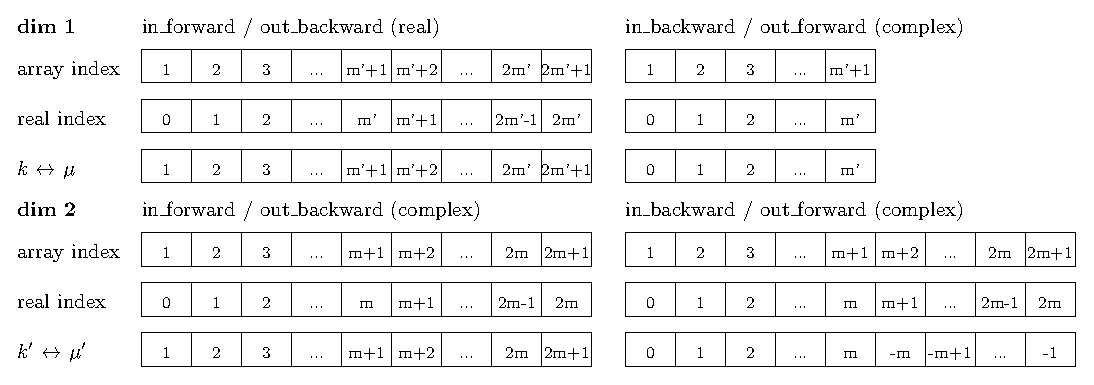
\includegraphics[width=1\textwidth]{_figure/fftw3_indices}
\par\end{center}
\begin{center}
\caption[Indices arrangement in a complete forward-backward FFT-2D process
of m'$\times$m elements]{Indices arrangement in a complete forward-backward \acs{FFT}-2D
process of m'$\times$m elements. The \acs{DFT} of dim 1 ($k$ to
$\mu$) and dim 2 ($j$ to $\mu'$) are done sequentially and \emph{vice
versa}. Array index is the one used by Fortran array, real index is
the one shown in eq. (\ref{eq:fftw3-fwd}) and (\ref{eq:fftw3-bwd}),
$k$ and $j$ indices shown in the left as well as $\mu$ and $\mu'$
in the right are those in eq. (\ref{eq:f_mup_mu}) and (\ref{eq:f_mup_mu_2}).
Here $\mathrm{m}=m_{\mathrm{max}}$ and $\mathrm{m}'=\left\lfloor m_{\mathrm{max}}/s\right\rfloor $.
\label{fig:FFTW3-2D-indices}}
\par\end{center}%
\end{minipage}
\end{figure}

As the output array of FFTW3 is periodic,
\begin{equation}
e^{2\pi i\mu k/n}=e^{2\pi i(\mu-n)k/n}e^{2\pi ik}=e^{2\pi i(\mu-n)k/n}\label{eq:mu-periodicity}
\end{equation}
the indices $\mu=m_{\mathrm{max}}+1,\ldots,2m_{\mathrm{max}}$ actually
correspond to $\mu=-m_{\mathrm{max}},\ldots,-1$. Note that eq. (\ref{eq:f_mup_mu})
and (\ref{eq:f_mup_mu_2}) do not possess the periodicity of eq. (\ref{eq:mu-periodicity}),
only in the domain of definition of $\mu'$ and $\mu$ some intermediary
functions share the same formula with \acs{FFT}.

Moreover, from eq. (\ref{eq:f_mup_mu}), (\ref{eq:f_mup_mu_3}) and
(\ref{eq:symm_f_m_mup_mu}), we can verify that
\begin{equation}
F_{\mu'\mu}(\Theta)=F_{\underline{\mu'}\underline{\mu}}^{*}(\Theta)
\end{equation}
The latter is used in the code since, according to the definition
in eq. (\ref{eq:fftw3-fwd}) and (\ref{eq:fftw3-bwd}), $F_{\underline{\mu'}\underline{\mu}}(\Theta)$
is calculated instead of $F_{\mu'\mu}(\Theta)$.

\section{Operational algorithm\label{sec:Operational-algorithm}}

As described above, the whole process of $\gamma$ and $\mathcal{F}_{\mathrm{exc}}$
functional evaluation proposed by this algorithm can be concluded
as 8 operations:
\begin{enumerate}
\item Firstly, the Fourier transform of the density is computed:
\begin{equation}
\Delta\hat{\rho}(\mathbf{k},\mathbf{\Omega})=\int\mathrm{d}\mathbf{r}\Delta\rho(\mathbf{r},\mathbf{\Omega})e^{-i\mathbf{k}\cdot\mathbf{r}}\label{eq:fft3d-fwd}
\end{equation}
\item Then $\Delta\hat{\rho}(\mathbf{k},\mathbf{\Omega})$ is expanded on
\acs{GSH}s:
\begin{equation}
\Delta\hat{\rho}_{\mu'\mu}^{m}(\mathbf{k})=\frac{f_{m}}{8\pi^{2}}\int\mathrm{d}\mathbf{\Omega}\Delta\hat{\rho}(\mathbf{k},\mathbf{\Omega})R_{\mu'\mu}^{m*}(\mathbf{\Omega})\label{eq:fgsht-fwd}
\end{equation}
Note that these two steps, the same with their backward transform,
are commutable, which will be discussed after.
\item Afterwards the projections in k-frame are then rotated into the local
coordinate system along the unit vector $\mathbf{\hat{k}}$:
\begin{equation}
\Delta\hat{\rho'}_{\chi\mu}^{m}(\mathbf{k})=\sum_{\mu'}\Delta\hat{\rho}_{\mu'\mu}^{m}(\mathbf{k})R_{\mu'\chi}^{m}(\mathbf{\hat{k}})\label{eq:2.2.rho-rot-rho}
\end{equation}
where the rotation matrix elements $R_{\mu'\chi}^{m}(\mathbf{\hat{k}})$
should be calculated directly because of the huge memory required
by its storage. The algorithm by recurrence used to evaluate $R_{\mu'\chi}^{m}(\mathbf{\hat{k}})$
in this thesis is detailed in appendix \ref{chpt:rotM-by-recurrence}.
\item Next, computing the OZ equation with Blum's reduction:
\begin{equation}
\hat{\gamma'}_{\chi\mu}^{m}(\mathbf{k})=\sum_{n,\nu}(-1)^{\chi+\nu}\hat{c'}_{\mu\nu,\chi}^{mn}(\mathbf{k})\Delta\hat{\rho'}_{\chi\underline{\nu}}^{n}(\mathbf{k})\label{eq:OZ-2}
\end{equation}
\item The $\gamma$ projections are then transformed back to global coordinates
system:
\begin{equation}
\hat{\gamma}_{\mu'\mu}^{m}(\mathbf{k})=\sum_{\chi}\hat{\gamma'}_{\chi\mu}^{m}(\mathbf{k})R_{\mu'\chi}^{m*}(\mathbf{\hat{k}})
\end{equation}
\item From here the function in angular frame can thus be rebuilt:
\begin{equation}
\hat{\gamma}(\mathbf{k},\mathbf{\Omega})=\sum_{m,\mu',\mu}f_{m}\hat{\gamma}_{\mu'\mu}^{m}(\mathbf{k})R_{\mu'\mu}^{m}(\mathbf{\Omega})\label{eq:fgsht-bwd}
\end{equation}
\item Then the inverse Fourier transform of these projections is:
\begin{equation}
\gamma(\mathbf{r},\mathbf{\Omega})=\int\mathrm{d}\mathbf{k}\hat{\gamma}(\mathbf{k},\mathbf{\Omega})e^{i\mathbf{r}\cdot\mathbf{k}}
\end{equation}
\item Finally, the functional $\mathcal{F}_{\mathrm{exc}}$ is computed
by:
\begin{equation}
\mathcal{F}_{\mathrm{exc}}=-\frac{k_{\mathrm{B}}T}{2}\int\mathrm{d}\mathbf{r}\mathrm{d}\mathbf{\Omega}\Delta\rho(\mathbf{r},\mathbf{\Omega})\gamma(\mathbf{r},\mathbf{\Omega})
\end{equation}
\end{enumerate}

\subsection{Commutativity between operations\label{subsec:Commutativity-between-operations}}

As mentioned in the operational algorithm, three types of operations
are being done before and after the \acs{OZ} equation. They are:
\begin{enumerate}
\item Fast Fourier transform for 3-dimensional spatial grid (\acs{FFT}3D):
implemented by package FFTW3 \citep{FFTW3}, mathematically leading
to no accuracy loss;
\item Fast generalized spherical harmonics transform (\acs{FGSHT}): has
real or complex input, is exact if $F(\mathbf{\Omega})$ can be given
as an expansion of \acs{GSH}s of order at most $m_{\mathrm{max}}$;
\item Rotation between laboratory coordinate system and local system linked
to vector $\mathbf{k}$ (RotS): can be done for both function and
projections. It introduces a minus error in accuracy at origin and
border of the box, which will be discussed in $\mathsection$\ref{subsec:k-border-effect}.
\end{enumerate}
Their commutativity is shown in figure \ref{fig:Commutativity-of-operations}.

\begin{figure}[h]
\begin{centering}
\includegraphics{_figure/algorithms_commutativity}
\par\end{centering}
\caption[Commutativity of operations]{Commutativity of operations. (a) FFT3D and FGSHT; (b) RotS and FGSHT;
(c) FFT3D and RotS.\label{fig:Commutativity-of-operations}}
\end{figure}

As shown in figure \ref{fig:Commutativity-of-operations}, the \acs{FFT}3D
does not depend on the angular part of the function, and the \acs{FGSHT}
does not depend on the spatial part of the function. The two operations
are commutative. 

It can be also proven that the passage from the function $\hat{f}$
in laboratory frame $\hat{f}(\mathbf{k},\mathbf{\Omega})$ to the
projections in local frame ${f'}_{\chi\mu}^{m}(\mathbf{k})$ can be
achieved either by a rotation to the function $\hat{f}(\mathbf{k},\boldsymbol{\omega}_{k})$
in intermolecular frame following by an \acs{GSH} expansion as eq.
(\ref{eq:gamma-projection-local}), or an \acs{GSH} expansion that
gives the projections $f_{\mu'\mu}^{m}(\mathbf{k})$ following by
a rotation as eq. (\ref{eq:gamma-p}).

However, the rotation from $f(\mathbf{r},\mathbf{\Omega})$ to $f(\mathbf{r},\boldsymbol{\omega})$
depends on the vector $\mathbf{r}$, of which the information is totally
lost after \acs{FFT}3D. The rotation from $f(\mathbf{k},\mathbf{\Omega})$
to $f(\mathbf{k},\boldsymbol{\omega})$ can only depend on the vector
$\mathbf{k}$; they are not the same rotation, therefore non-commutative. 

\subsection{Reduction by symmetry\label{subsec:Reduction-by-symmetry}}

A further reduction of computing cost can be made by performing about
only half of the operations, thanks to the symmetric relations between
the projections.

In eq. (\ref{eq:fgsht-fwd}), $\Delta\rho(\mathbf{r},\mathbf{\Omega})$
is real. With the property of \acs{GSH} (eq. (\ref{eq:symm-gsh-1})):
\begin{equation}
R_{\mu'\mu}^{m}(\mathbf{\Omega})=(-)^{\mu'+\mu}R_{\underline{\mu'}\underline{\mu}}^{m*}(\mathbf{\Omega})
\end{equation}
we find
\begin{equation}
\Delta\hat{\rho}_{\mu'\mu}^{m}(\mathbf{r})=(-)^{\mu'+\mu}\Delta\hat{\rho}_{\underline{\mu'}\underline{\mu}}^{m*}(\mathbf{r})\label{eq:2.2.symm-rho-r}
\end{equation}
Therefore only the projections of $\mu'\geq0$ or $\mu\geq0$ are
needed to generate all information.

When $\Delta\hat{\rho}_{\mu'\mu}^{m}(\mathbf{r})$ is transformed
into $k$-space, replacing
\begin{equation}
\Delta\hat{\rho}_{\mu'\mu}^{m}(\mathbf{k})=\int\mathrm{d}\mathbf{r}\Delta\rho_{\mu'\mu}^{m}(\mathbf{r})e^{-i\mathbf{r}\cdot\mathbf{k}}
\end{equation}
 with eq. (\ref{eq:2.2.symm-rho-r}) gives
\begin{equation}
\Delta\hat{\rho}_{\mu'\mu}^{m}(\mathbf{k})=(-)^{\mu'+\mu}\Delta\hat{\rho}_{\underline{\mu'}\underline{\mu}}^{m*}(-\mathbf{k})\label{eq:2.2.symm-rho-k}
\end{equation}
Therefore only the projections of $\mu'\geq0$, $\mu\geq0$, or a
half of $\mathbf{k}$ where one of the dimensions $k_{i}\geq0$ are
independent. 

In the implementation, it is a natural choice to keep only a half
of projections $\Delta\hat{\rho}_{\mu'\mu}^{m}(\mathbf{k})$, as either
the real-to-complex \acs{FFT}3D ($k_{3}\geq0$) or the real-to-complex
\acs{FGSHT} ($\mu\geq0$) gives implicitly a half of information.
As the \acs{OZ} equation (\ref{eq:gamma-blum}) is separable for
each $\mathbf{k}$, but not on $\mu$ ($\nu$ in equation), it is
more natural compute a half of $\mathbf{k}$, which is actually the
choice in our code. All the rest we should prove is that the $\hat{\gamma}_{\mu'\mu}^{m}(\mathbf{k})$
calculated from this half of known density is still able to generate
all the informations.

The relation deduced from the symmetries of \acs{GSH} (appendix \ref{chpt:symmetry}):
\begin{equation}
r_{\mu'\mu}^{m}(\theta)=(-)^{m+\mu'}r_{\mu'\underline{\mu}}^{m}(\pi-\theta)
\end{equation}
\begin{eqnarray}
R_{\mu'\mu}^{m}(\phi\theta\psi) & = & (-)^{m+\mu'}e^{i\mu'\pi}R_{\mu'\underline{\mu}}^{m}(\pi+\phi,\pi-\theta,-\psi)\\
 & = & (-)^{m}R_{\mu'\underline{\mu}}^{m}(\pi+\phi,\pi-\theta,-\psi)
\end{eqnarray}
gives that
\begin{equation}
R_{\lambda'0}^{l}(\hat{\mathbf{k}})=(-)^{l}R_{\lambda'0}^{l}(-\hat{\mathbf{k}})=(-)^{l+\lambda'}R_{\underline{\lambda'}0}^{l*}(-\hat{\mathbf{k}})\label{eq:2.2.symm-lambda}
\end{equation}

If we replace eq. (\ref{eq:im}) by eq. (\ref{eq:2.2.symm-rho-k})
and (\ref{eq:2.2.symm-lambda}), with symmetry of 3j-symbol (\ref{eq:symm-3j-symbol})
and symmetry of $\hat{c}$ \citep{Blum_I}:
\begin{equation}
\hat{c}_{\mu\nu}^{mnl}(k)=\left(-\right)^{m+n+\mu+\nu}\hat{c}_{\underline{\mu}\underline{\nu}}^{mnl*}(k)
\end{equation}
we have the same symmetry property for $\hat{\gamma}$ as for $\Delta\hat{\rho}$:
\begin{equation}
\hat{\gamma}_{\mu'\mu}^{m}(\mathbf{k})=\left(-\right)^{\mu'+\mu}\hat{\gamma}_{\underline{\mu'}\underline{\mu}}^{m*}(-\mathbf{k})
\end{equation}
which means the half $\hat{\gamma}_{\mu'\mu}^{m}(\mathbf{k})$ is
sufficient to generate $\hat{\gamma}(\mathbf{k},\mathbf{\Omega})$
or $\gamma(\mathbf{r},\mathbf{\Omega})$. Thus the \acs{OZ} equation
can be safely reduced by a factor of two. 

We can also find
\begin{equation}
R_{\mu'\chi}^{m}(\hat{\mathbf{k}})=(-)^{m}R_{\mu'\underline{\chi}}^{m}(-\hat{\mathbf{k}})=(-)^{m+\mu'+\chi}R_{\underline{\mu'}\chi}^{m}(-\hat{\mathbf{k}})\label{eq:3}
\end{equation}
which gives
\begin{equation}
\Delta\hat{\rho'}_{\chi\mu}^{m}(\mathbf{k})=(-)^{m+\mu+\chi}\Delta\hat{\rho'}_{\chi\underline{\mu}}^{m*}(-\mathbf{k})
\end{equation}
\begin{equation}
\hat{\gamma'}_{\chi\mu}^{m}(\mathbf{k})=(-)^{m+\mu+\chi}\hat{\gamma'}_{\chi\underline{\mu}}^{m*}(-\mathbf{k})
\end{equation}

If we replaced the \acs{OZ} equation by these two equations, we can
find the symmetries of $\hat{c'}_{\mu\nu,\chi}^{mn}(k)$ in eq. (\ref{eq:rot-invar-symm-k-chi}):
\begin{equation}
\hat{c}_{\mu\nu,\chi}^{mn}(k)=\left(-\right)^{m+n+\mu+\nu}\hat{c}_{\underline{\mu}\underline{\nu},\chi}^{mn*}(k)
\end{equation}

It should be noted that not exactly the half of points are calculated.
If we choose to calculate a half of $\mathbf{k}$, as shown in figure
\ref{fig:points-symm}, where the 2D plan corresponds two of the three
dimensions in $k$-space grid, the green points can be generated from
the black points by the symmetries of eq. (\ref{eq:2.2.symm-rho-k}),
but the red points should be all calculated, of which the corresponding
points is also a red point or even itself. This ever caused a huge
problem in the implementation, as we put $\Delta\hat{\rho}_{\mu'\mu}^{m}(\mathbf{k})$
and $\hat{\gamma}_{\mu'\mu}^{m}(\mathbf{k})$ in the same array for
reason of memory. It should be assured that these points are calculated
only once.

\begin{figure}[th]
\begin{centering}
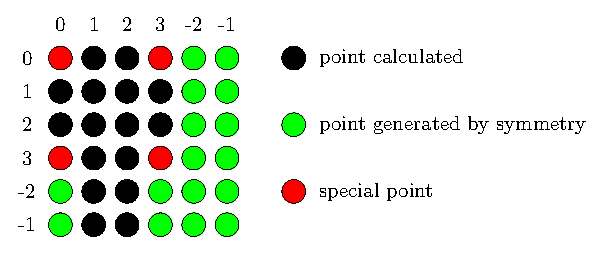
\includegraphics{_figure/test_lmn}
\par\end{centering}
\caption{Distribution of points to be calculated according to symmetry in a
2D plan\label{fig:points-symm}}
\end{figure}




\chapter{Free Energy and Related Thermodynamic Quantities\label{chpt:thermodynamic-quantities}}

The solvation free energy is the most important property that we seek;
as shown in previous sections, it can be calculated by the minimization
of free energy functional $\mathcal{F}[\rho]$. Here is a discussion
about some corrections needed for charged solutes and some related
thermodynamic quantities that can be obtained directly from the solvation
free energy.

The solvation properties often involve the three-dimensional microscopic
structure of the solvent around the dissolved molecule, as well as
thermodynamic quantities such as the enthalpy, entropy, and free
energy of solvation {[}ref gubbins{]} pKa {[}ref{]}.

The solvation properties can be determined if the two principle properties, free energy and structure,
are accurately calculated. In this thesis,
we focus on these two aspects.


\section{Free energy correction for a single ion}

In the calculation of external potential as well as the total solvation
free energy, the use of different conventions can lead to a charge-independent
offset, which introduces error for charged solutes \citep{Kastenholz_2006_I,Kastenholz_2006_II,Hunenberger_book}.
This offset is mainly caused by two sources: (1) resulting from the use of
a finite system size; in our case, a system with cubic periodic
boundary conditions, which presents artificial interactions between
the ion and its own periodic copies, as well as between the solvent
and the periodic copies of the ion (Type-B in \citep{Kastenholz_2006_II});
(2) owing to the choice of convention for summing up the contributions
of solvent charges to the electrostatic potential in the sample system
(Type-C in \citep{Kastenholz_2006_II}).


\subsection{Correction of type B}

Type B correction should be added for systems with finite size or
periodic boundary conditions, accounting for the error in the solvent
polarization \marginpar{Another way to evaluate this error is to make a numerical extrapolation
of the inverse of the box size $\left(1/L\right)$; it is more accurate
but demands much more calculation.}
\begin{equation}
\Delta G_{B}=\frac{1}{8\pi\varepsilon_{0}}\left(1-\varepsilon^{-1}\right)\frac{q^{2}}{L}\left[\xi+\frac{4\pi}{3}\left(\frac{R_{\mathrm{I}}}{L}\right)^{2}-\frac{16\pi}{45}\left(\frac{R_{\mathrm{I}}}{L}\right)^{5}\right]\label{eq:corr-B}
\end{equation}
where

\begin{tabular}{cl}
 $\varepsilon_{0}$ & is the vacuum permittivity;\tabularnewline
$\varepsilon$ is the solvent permittivity (dielectric constant);\tabularnewline
$q$ & is the solute charge;\tabularnewline
$L$ & \textcolor{red}{is the box length};\tabularnewline
$R_{\mathrm{I}}$ & is the ionic radius;\tabularnewline
$\xi$ & \textcolor{red}{is the energy per particle in a simple cubic lattice,}
$\xi\simeq-2.837297$ \citep{nijboer}.\tabularnewline
 & \tabularnewline
\end{tabular} 

As $R_{\mathrm{I}}$ is significantly smaller than the size of the
computational box, i. e. $R_{\mathrm{I}}\ll L$, its quadratic as
well as higher order of $\left(R_{\mathrm{I}}/L\right)$ is considered
negligible, thus eq. (\ref{eq:corr-B}) becomes
\begin{equation}
\Delta G_{\mathrm{B}}=\frac{\xi}{8\pi\varepsilon_{0}}\left(1-\varepsilon^{-1}\right)\frac{q^{2}}{L}
\end{equation}
\textcolor{red}{It links to Born correction}.


\subsection{Correction of type C}

Type-C corrections are needed when the systems to be compared use different
electrostatic summation schemes: on the basis of point charges within
entire solvent molecules (M scheme) or on the basis of individual
point charges (P scheme), shown in figure \ref{fig:IQ-model-som-scheme}
(c) and (d), which brings a fixed free energy difference at the boundary.

\begin{figure}[h]
\begin{centering}
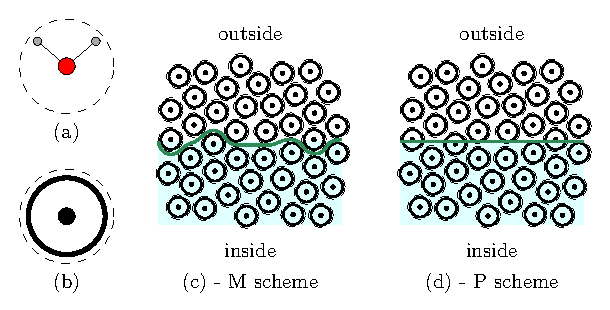
\includegraphics{_figure/ion_correction}
\par\end{centering}

\caption [IQ model and summation scheme]{IQ model and summation scheme. (a) The solvent molecule. (b) The
equivalent isotropic quadrupole (IQ) fluid model. (c) In the M scheme,
one evaluates the Coulombic potential generated by the solvent charges
belonging to all molecules within the boundary. (d) In the P scheme,
one evaluates the Coulombic potential generated by all solvent charges
within the boundary.\label{fig:IQ-model-som-scheme}}
\end{figure}


It can be deduced analytically by considering the solvent as a \textcolor{red}{canonical
ensemble} under the orientational disorder limit (ODL) \citep{Kastenholz_2006_I},
which becomes an isotropic quadrupole (IQ) fluid, whose solvent molecule
(figure \ref{fig:IQ-model-som-scheme} (b)) possesses the same quadrupole
trace $\gamma$ \marginpar{$\gamma$ which is elsewhere referred to as the spheropole moment \citep{Saunders_1992,Maschio_2012},
that is, the spherical component of the quadrupole moment, and is
invariant with respect to rotations.}
\begin{equation}
\gamma=\mathrm{tr}(\mathbf{\mathcal{Q}})=\mathcal{Q}_{xx}+\mathcal{Q}_{yy}+\mathcal{Q}_{zz}
\end{equation}
where the quadrupole moment of the solvent molecule can be calculated
by its definition \citep{Multipole}:
\begin{equation}
\mathcal{Q}_{ij}=\int_{V}r_{i}r_{j}\rho(\mathbf{r})\mathrm{d}v=\sum_{\alpha=1}^{N}q^{(\alpha)}r_{i}^{(\alpha)}r_{j}^{(\alpha)}
\end{equation}


It can be shown that the charge density of a solvent located within the
boundary of a sample system vanishes everywhere except at the boundary
in the M scheme, which results in a uniform normal surface polarization.
The correction needed for\textcolor{red}{{} M scheme }is
\begin{equation}
\Delta G_{\mathrm{C}}=-q\left(1-\frac{4\pi R_{\mathrm{I}}^{3}}{3L^{3}}\right)\Delta\Phi_{\mathrm{ODL}}\label{eq:corr-C}
\end{equation}
where $\Delta\Phi_{\mathrm{ODL}}=\left(6\varepsilon_{0}\right)^{-1}\eta\gamma$,
$\eta$ being the solvent number density.

In the same way, when we consider $R_{\mathrm{I}}\ll L$, eq. (\ref{eq:corr-C})
becomes
\begin{equation}
\Delta G_{\mathrm{C}}=-\left(6\varepsilon_{0}\right)^{-1}\eta\gamma q
\end{equation}



\section{Some related thermodynamic quantities}

\textquotedbl{}expansion work\textquotedbl{} term PV

Thermodynamic quantities such as the internal energy, pressure, compressibility
and heat capacity are obtained as derivatives of the classical partition
function. {[}Evans poly{]}

Structure and Thermodynamic Properties of Bulk Liquids

Pressure is (virial pressure equation) 
\begin{equation}
p=\rho k_{\mathrm{B}}T-\dfrac{\rho^{2}}{2}\int\mathrm{d}\mathbf{r}g(r)\frac{r}{3}\frac{\mathrm{d}u(r)}{\mathrm{d}r}
\end{equation}


The Gibbs free energy G is simply {[}Evans 1979{]}.

$G=\mu\int\mathrm{d}\mathbf{r}\rho(\mathbf{r})$


\subsection{Solubility}


\subsection{Pressure}

enthalpy, entropy {[}3{]} pH



\chapter{Solvation Structure\label{chpt:solvation-structure}}

In MDFT, all the information about solvation structure can be deduced
from the solvent density $\rho(\mathbf{r},\mathbf{\Omega})$. This
section presents some examples of structure which are used in later
chapters.

\section{Radial distribution function and site-site distribution function}

When the solvent is homogeneous, the \acs{PDF} can be reduced to
$g(r_{12})$, which is sometimes referred to as the radial distribution
function (\acs{RDF}). However, it is also used as a key character
of the structure for inhomogeneous fluids, which can be calculated
equivalently as:
\begin{equation}
g(r)=\left\langle \rho(r,\hat{\mathbf{r}})\right\rangle =\dfrac{\int\rho(r,\hat{\mathbf{r}})\mathrm{d}s_{r}}{\int\mathrm{d}s_{r}}
\end{equation}

To do this integration, it is required to transform $\rho(\mathbf{r},\mathbf{\Omega})$
into spherical coordinates. But as $\rho(\mathbf{r},\mathbf{\Omega})$
in the code is a $N$-point discrete space grid:
\begin{equation}
\rho(\mathbf{r})=\int\mathrm{d}\mathbf{\Omega}\rho(\mathbf{r},\mathbf{\Omega})=\sum_{i=1}^{N}\rho_{i}\delta(\mathbf{r}-\mathbf{r}_{i})
\end{equation}
The best way to do the integration is to use a histogram approach.

The grid points are assumed to be homogenous in space, such that the
number of points entering in an arbitrary volume $v$ is proportional
to this volume. Obviously the grid of $\rho(\mathbf{r},\mathbf{\Omega})$
satisfies this assumption.

The average value of $g(r)$ between an interval $\delta r$ is
\begin{equation}
g(r_{i})=\left\langle g(r)\right\rangle _{r}^{r+\delta r}=\dfrac{\int_{r}^{r+\delta r}g(r)\mathrm{d}r}{\delta r}
\end{equation}

Thus
\begin{equation}
g(r_{i})=\dfrac{1}{\delta v_{i}}\int_{r}^{r+\delta r}\int_{s}\rho(r,\hat{\mathbf{r}})\mathrm{d}r\mathrm{d}s_{r}=\dfrac{1}{\delta v_{i}}\int_{v_{i}}\sum_{i=1}^{N}\rho_{i}\delta(\mathbf{r}-\mathbf{r}_{i})\mathrm{d}v_{i}
\end{equation}
where $\delta v_{i}=\delta r\cdot s_{r_{i}}=\int_{v_{i}}\delta(\mathbf{r}-\mathbf{r}_{i})\mathrm{d}v_{i}$
(as the points are homogeneous). 

The total function is 
\begin{equation}
g(r_{i})=\dfrac{\int_{v_{i}}\sum_{i=1}^{N}\rho_{i}\delta(\mathbf{r}-\mathbf{r}_{i})\mathrm{d}v_{i}}{\int_{v_{i}}\delta(\mathbf{r}-\mathbf{r}_{i})\mathrm{d}v_{i}}
\end{equation}
and it becomes necessary to sum up the point values $\rho_{i}$ in the interval
$\delta v=\delta r\cdot S_{r}$, and divide it by the number of points
in this interval.

A site-site distribution function is the same type as \acs{RDF},
but the origin for the calculation of $\mathbf{r}$ is no longer at
the center of the solute, but is now at the site coordinate $\mathbf{r}_{u}$, such
that the new coordinates are calculated as $\mathbf{r}'=\mathbf{r}-\mathbf{r}_{u}$.
Calculation of solvent site outside the solvent center requires more
complicated calculations, involving the rotation of solvent coordinate
to $\mathbf{\Omega}$-frame. It has equivant information of the structure
to the rotational invariant projections of higher order, the implementation of which
we have not done here.

\section{Radial polarization functions}

Radial polarization function (RPF) is defined as 
\begin{equation}
p(r)=\left\langle P(r,\hat{\mathbf{r}})\right\rangle 
\end{equation}
where $P(\mathbf{r})$ is the polarization $P(\mathbf{r})=\int\mathbf{\Omega}\cdot\rho(\mathbf{r},\mathbf{\Omega})\mathrm{d}\mathbf{\Omega}$.
It can be calculated in the same way as $g(r)$.

\section{Rotational invariant expansion}

The density can be expanded on rotational invariants:
\begin{eqnarray}
\rho(\mathbf{r},\mathbf{\Omega}) & = & \sum_{mnl\mu\nu}\rho_{\mu\nu}^{mnl}(r)\Phi_{\mu\nu}^{mnl}(0,\mathbf{\Omega},\mathbf{\hat{r}})\label{eq:rot_invar_expansion}\\
 & = & \sum_{mnl\mu\nu}\rho_{\mu\nu}^{mnl}(r)f^{m}f^{n}\sum_{\eta}\left(\begin{array}{ccc}
m & n & l\\
\mu & \eta & -\mu-\eta
\end{array}\right)R_{\eta\nu}^{n}(\mathbf{\Omega})R_{-\mu-\eta,0}^{l}(\mathbf{\hat{r}})
\end{eqnarray}

The forward transform is shown below:
\begin{equation}
\rho_{\mu\nu}^{mnl}(r)=f^{m}f^{n}\sum_{\eta}\left(\begin{array}{ccc}
m & n & l\\
\mu & \eta & -\mu-\eta
\end{array}\right)\int\mathrm{d}\hat{\mathbf{r}}R_{-\mu-\eta,0}^{l*}(\mathbf{\hat{r}})\int\mathrm{d}\mathbf{\Omega}\rho(r,\hat{\mathbf{r}},\mathbf{\Omega})R_{\eta,\nu}^{n*}(\mathbf{\Omega})
\end{equation}

A detailed deduction for this generalized formula is in appendix \ref{chpt:rotational-invariant-expansion}.

\section{Equivalence between the curves}

The relation between these curves can be proven mathematically.

Firstly, as
\begin{equation}
\Phi_{00}^{000}(\mathbf{r},\mathbf{\Omega})=1
\end{equation}
there is only one expansion term in eq. (\ref{eq:rot_invar_expansion}).
The projection is
\begin{equation}
\rho_{00}^{000}(r)=\rho(\mathbf{r},\mathbf{\Omega})=g(r)
\end{equation}

Then,
\begin{eqnarray}
\Phi_{00}^{011}(\mathbf{r},\mathbf{\Omega}) & = & \sqrt{3}\left(\begin{array}{ccc}
0 & 1 & 1\\
0 & 0 & 0
\end{array}\right)R_{00}^{1}(\mathbf{\Omega})R_{00}^{1}(\mathbf{\hat{r}})\nonumber \\
 & + & \sqrt{3}\left(\begin{array}{ccc}
0 & 1 & 1\\
0 & 1 & -1
\end{array}\right)R_{10}^{1}(\mathbf{\Omega})R_{-10}^{1}(\mathbf{\hat{r}})\nonumber \\
 & + & \sqrt{3}\left(\begin{array}{ccc}
0 & 1 & 1\\
0 & -1 & 1
\end{array}\right)R_{-10}^{1}(\mathbf{\Omega})R_{10}^{1}(\mathbf{\hat{r}})
\end{eqnarray}
such that
\begin{eqnarray}
\Phi_{00}^{011}(\mathbf{r},\mathbf{\Omega}) & = & -3R_{00}^{1}(\mathbf{\Omega})R_{00}^{1}(\mathbf{\hat{r}})\nonumber \\
 & + & 3R_{10}^{1}(\mathbf{\Omega})R_{-10}^{1}(\mathbf{\hat{r}})\nonumber \\
 & + & 3R_{-10}^{1}(\mathbf{\Omega})R_{10}^{1}(\mathbf{\hat{r}})\\
 & = & -3\mathbf{\Omega}\cdot\hat{\mathbf{r}}
\end{eqnarray}
with $R_{00}^{1}(\mathbf{\Omega})=\cos\theta$ and $R_{10}^{1}(\mathbf{\Omega})=-\frac{1}{\sqrt{2}}\sin\theta e^{-i\phi}$.

We can see
\begin{equation}
\rho_{00}^{011}(r)=\dfrac{\int\mathrm{d}\hat{\mathbf{r}}\mathrm{d}\mathbf{\Omega}\rho(\mathbf{r},\mathbf{\Omega})\Phi_{00}^{011*}(\mathbf{r},\mathbf{\Omega})}{\int\mathrm{d}\hat{\mathbf{r}}\mathrm{d}\mathbf{\Omega}\left\Vert \Phi_{00}^{011}(\mathbf{r},\mathbf{\Omega})\right\Vert ^{2}}=-\dfrac{1}{3}\dfrac{\int\mathrm{d}\hat{\mathbf{r}}P(\mathbf{r})\cdot\hat{\mathbf{r}}}{\int\mathrm{d}\hat{\mathbf{r}}\mathrm{d}\mathbf{\Omega}\left\Vert \mathbf{\Omega}\cdot\hat{\mathbf{r}}\right\Vert ^{2}}
\end{equation}
... (yes, in the implementation we see they are different curves.
No exact equivalence.)


\ctparttext{The code MDFT developed in this thesis is based on the branch master
of Git project MDFT (\url{https://github.com/maxlevesque/MDFT/}),
version {[}Fri Jun 20 19:05:52 2014 +0200{]}. All the implementations
are run on \textsf{\textbf{POINCARE}} machines of IDRIS, which involved
two kinds of machines:\\
\medskip{}
\textsf{\textbf{poincare{[}001-092{]}:}} 2 processors Sandy Bridge
E5-2670 (2.60GHz, 8 cores per processor, being 16 cores per node);
32 GB of memory per node.\\
\medskip{}
\textsf{\textbf{poincarebig{[}01-02{]}:}} 4 processors AMD Opteron
6282 (2.60GHz, 16 cores per processor, being 64 cores per node); 128
GB of memory per node.\\
\medskip{}
The former is used for regular calculation, whose memory hierarchy
is shown in figure \ref{fig:poincare}. The later is only used in
the evaluation of accuracy, in case of memory leak in the former.\\
\medskip{}
\begin{figure}[h]
\begin{centering}
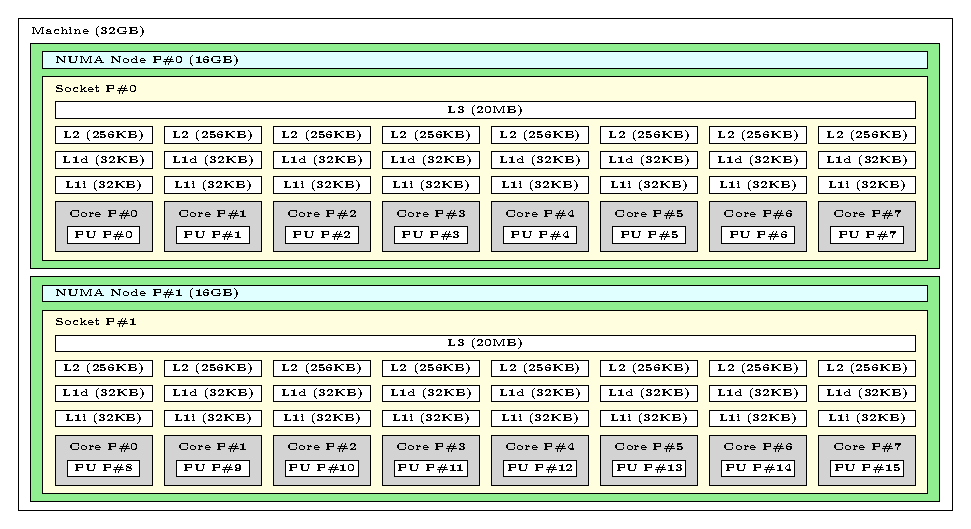
\includegraphics[width=0.9\columnwidth]{_figure/poincare}
\par\end{centering}
\caption{Structure of a POINCARE node\label{fig:poincare}}
\end{figure}
\medskip{}
Section \ref{chpt:algorithms-and-branches}, gives a brief introduction
of all the implementation algorithms built in this thesis.\\
\medskip{}
Section \ref{chpt:accuracy} compares the accuracy of each algorithm,
from parts of the code to entire branches.\\
\medskip{}
Section \ref{chpt:seq-code-performance} computing performance and
memory limits for the sequential code. Due to the time limit, the
parallelized version has not been totally built, it is put in the
perspectives. }

\part{Implementation}


\chapter{Algorithms and Branches\label{chpt:algorithms-and-branches}}

According to the commutativity of operations (see $\mathsection$\ref{subsec:Commutativity-between-operations}),
the only possible algorithms to evaluate $\gamma(\mathbf{r},\mathbf{\Omega})$
from $\Delta\rho(\mathbf{r},\mathbf{\Omega})$ are shown in the figure
\ref{fig:Possible-algorithms}.

\begin{figure}[h]
\begin{centering}
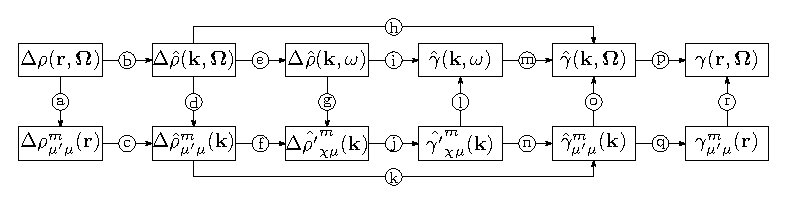
\includegraphics{_figure/algorithms}
\par\end{centering}
\caption{Possible algorithms for $\gamma$ evaluation\label{fig:Possible-algorithms}}
\end{figure}

Several branches are built to test and compare between algorithms,
which are shown below in table \ref{tab:Branch-option} and will be
detailed in the following context. \marginpar{These branches should give numerically the same result in certain
conditions, that will be discussed in later sections.}

\selectlanguage{english}%
\begin{table}[h]
\selectlanguage{american}%
\begin{centering}
\begin{tabular*}{1\textwidth}{@{\extracolsep{\fill}}cccc}
\toprule 
\tableheadline{Method} & \tableheadline{Sub-Method} & \tableheadline{Description} & \tableheadline{Theory}\tabularnewline
\midrule
reference & dipole & calculate $n(r)$ and $P(r)$ separately & $\mathsection$\ref{chpt:mdft} \textcolor{red}{{[}ref{]}}\tabularnewline
\midrule
naive & standard & use $c_{\mu\nu,\chi}^{mn}(k)$ as input DCF & $\mathsection$\ref{subsec:Using-projections-in-1}\tabularnewline
 & zero-order & use $\hat{c}(k,\boldsymbol{\omega_{1}},\boldsymbol{\omega_{2}})$
and take the nearest point & $\mathsection$\ref{subsec:Zero-order-interpolation-of}\tabularnewline
 & interpolation & use $\hat{c}(k,\boldsymbol{\omega_{1}},\boldsymbol{\omega_{2}})$
with linear interpolation  & $\mathsection$\ref{subsec:Linear-interpolation-of}\tabularnewline
 & dipole & use $c_{S}$, $c_{\Delta}$, $c_{D}$ issue from \textcolor{red}{{[}ref{]}} & $\mathsection$\ref{subsec:Using-projections-in}\tabularnewline
 & nmax1 & use $c_{S}$, $c_{\Delta}$, $c_{D}$, $c_{\pm}$ issue from {\footnotesize{}\citep{puibasset_bridge_2012}} & $\mathsection$\ref{subsec:Using-projections-in}\tabularnewline
\midrule
convolution & standard & algorithm with symmetry reduction & $\mathsection$\ref{subsec:Reduction-by-symmetry}\tabularnewline
 & asymm  & algorithm without symmetry reduction & $\mathsection$\ref{subsec:Reduction-by-symmetry}\tabularnewline
 & pure\_angular  & inverse FFT and FGSHT & $\mathsection$\ref{chpt:algorithms-and-branches}\tabularnewline
\bottomrule
\end{tabular*}
\par\end{centering}
\selectlanguage{english}%
\caption{\foreignlanguage{american}{Branch option in MDFT\label{tab:Branch-option}}}
\end{table}

\selectlanguage{american}%

\section{Branches \textquotedbl{}naive\textquotedbl{} }

Branches \texttt{\textbf{naive}} are the algorithms mentioned in section
\ref{chpt:fft-spatial}, which go through the path 
\[
\left(b\right)\shortrightarrow\left(h\right)\shortrightarrow\left(p\right)
\]
 in figure \ref{fig:Possible-algorithms}, calculating directly $\hat{\gamma}(\mathbf{k},\mathbf{\Omega})$
from $\Delta\hat{\rho}(\mathbf{k},\mathbf{\Omega})$. The difference
between branches is the way to calculate $\hat{c}(\mathbf{k},\mathbf{\Omega_{1}},\mathbf{\Omega_{2}})$.
Branch\textbf{ }\texttt{\textbf{naive\_standard}} use $c_{\mu\nu,\chi}^{mn}(k)$
as input \acs{DCF}. Branch \texttt{\textbf{naive\_zero-order}} and
\texttt{\textbf{naive\_interpolation}} using $\hat{c}(k,\boldsymbol{\omega_{1}},\boldsymbol{\omega_{2}})$
with zero-order and linear interpolation, where the former is rejected
in the implementation due to a lack of precision (appendix \ref{chpt:error-evaluation-interpolation-DCF}).

\section{Branches \textquotedbl{}convolution\textquotedbl{}}

Branches\textbf{ }\texttt{\textbf{convolution\_asymm}} and \texttt{\textbf{convolution\_standard}}
are operational algorithms of angular convolution show in section
\ref{chpt:angular-convolution}, which go through the path 
\[
\left(a\right)\shortrightarrow\left(c\right)\shortrightarrow\left(f\right)\shortrightarrow\left(j\right)\shortrightarrow\left(n\right)\shortrightarrow\left(q\right)\shortrightarrow\left(r\right)
\]

Branches\textbf{ }\texttt{\textbf{convolution\_asymm}} uses the original
operational algorithm ($\mathsection$\ref{sec:Operational-algorithm})
without symmetry reduction ($\mathsection$\ref{subsec:Reduction-by-symmetry}),
and \texttt{\textbf{convolution\_standard}} with it. 

Branch \texttt{\textbf{convolution\_pure\_angular}} goes through the
path 
\[
\left(b\right)\shortrightarrow\left(d\right)\shortrightarrow\left(f\right)\shortrightarrow\left(j\right)\shortrightarrow\left(n\right)\shortrightarrow\left(o\right)\shortrightarrow\left(p\right)
\]
which inverse the first and last two steps of the two algorithms mentioned
above.

\section{Testing branches for $n_{\max}$=1}

Branches \texttt{\textbf{naive\_dipole}}, \texttt{\textbf{naive\_nmax1}}
pass by $\left(b\right)\shortrightarrow\left(h\right)\shortrightarrow\left(p\right)$
, using DCF separately of the references \textcolor{red}{{[}ref{]}}
and {\footnotesize{}\citep{puibasset_bridge_2012}}, whose slight
difference is shown in $\mathsection$\ref{subsec:Comparison-with-non-coupling}.
Branch \texttt{\textbf{reference\_dipole}} use DCF in \textcolor{red}{{[}ref{]}},
which is the original method in MDFT to calculate $\mathcal{F}_{\mathrm{exc}}$
via multipole expansion. In addition with branch \texttt{\textbf{convolution\_standard}},
which can also use the two DCF mentioned above, a test of validation
can be performed, which should at any case exactly numerically the
same if the same DCF is used.

\section{Other paths}

Considering the necessity, other paths such as those passing by $\left(i\right)$
and $\left(k\right)$ are only built for local test usage (c. f. discussion
in following sections).



\chapter{Numerical and Physical Accuracy\label{chpt:accuracy}}

This chapter gives a systematic comparison between algorithms for
the evaluation of the excess free energy $\mathcal{F}_{\mathrm{exc}}$
and its gradient $\gamma$ in terms of accuracy. As the theory does
not contain any unpredictable random part, the comportment of the
code is mathematically predictable. For example, certain algorithms
should give the same result at machine precision ($10^{-13}$ to $10^{-15}$)
in certain conditions. A loss of accuracy comparing to the prediction
can be classified as two different types. One is the theoretical loss;
for instance, a certain equation is only valid for an infinite order.
This kind of loss is unavoidable but should be worked out explicitly.
Another source is the unknown loss, containing all kinds of incompatibility
in the result that cannot be explained mathematically. It is mainly attributable to a bug in the implementation that cannot be located. There is also the possibility that it is a theoretical loss which has not been worked out. All these comparisons aim to give a global view of the credibility for the results given by this code.

\section{Generalized spherical harmonics transform\label{sec:gsh-imp}}

As discussed in $\mathsection$\ref{sec:fgsht}, the function after
a forward-backward \acs{GSHT} process 
\begin{equation}
F_{\mu'\mu}^{m}=\frac{f_{m}}{8\pi^{2}}\sum_{i=0}^{m_{\mathrm{max}}}w_{i}\sum_{j=0}^{2m_{\mathrm{max}}}\sum_{k=0}^{2\left\lfloor m_{\mathrm{max}}/s\right\rfloor }F(\Theta_{i},\Phi_{j},\Psi_{k})R_{\mu'\mu}^{m*}(\Theta_{i},\Phi_{j},\Psi_{k})
\end{equation}
\begin{equation}
F(\Theta_{i},\Phi_{j},\Psi_{k})=\sum_{m=0}^{n_{\mathrm{max}}}f_{m}\sum_{\mu'=-m}^{m}\sum_{\underset{\mod(\mu,s)=0}{\mu=-m}}^{m}F_{\mu'\mu}^{m}R_{\mu'\mu}^{m}(\Theta_{i},\Phi_{j},\Psi_{k})
\end{equation}
only remains the same when it is a polynomial of both $\cos\Theta$,
$\cos\Phi$ and $\cos\Psi$ of order $n_{\max}$, where $n_{\max}$
is the highest order of \acs{GSH} in the expansion, and $m_{\max}=n_{\max}$
the order of quadrature used. However, as in reality, the density
variable $\rho$ is not a simple polynomial, and the choice of $m_{\max}$
and $n_{\max}$ is tightly linked to the performance. It is important
to know how much these choices will affect the results. The \acs{FFT}
process is implemented by package FFTW3 \citep{FFTW3}, which is verified
to be leading to strictly no accuracy lost (at machine precision).
That means the \acs{FGSHT} process will have strictly with the \acs{GSHT} %'will have strictly'? Something is missing.
process. Here we do not need to distinguish the two.

\subsection{$m_{\mathrm{max}}$ and $n_{\mathrm{max}}$ of projections}

The numerical error tests of a forward-backward GSHT process with
different order $n_{\mathrm{max}}$ of GSH and $m_{\mathrm{max}}$
of quadrature are shown in table \ref{tab:error-gsh}.
\begin{table}[H]
\begin{centering}
\subfloat[$f(\mathbf{\Omega})=1$]{\begin{centering}
\begin{tabular*}{1\columnwidth}{@{\extracolsep{\fill}}ccccccc}
\toprule 
{\footnotesize{}$m$\textbackslash{}$n$} & \multirow{1}{*}{{\footnotesize{}0}} & \multirow{1}{*}{{\footnotesize{}1}} & {\footnotesize{}2} & \multirow{1}{*}{{\footnotesize{}3}} & \multirow{1}{*}{{\footnotesize{}4}} & \multirow{1}{*}{{\footnotesize{}5}}\tabularnewline
\midrule
\multicolumn{1}{c}{{\footnotesize{}0}} & \textbf{\footnotesize{}0 (0)} & {\footnotesize{}9.00 (3.00)} & {\footnotesize{}34.00 (18.00)} & {\footnotesize{}83.00 (39.00)} & {\footnotesize{}164.00 (84.00)} & {\footnotesize{}285.00 (139.00)}\tabularnewline
\multicolumn{1}{c}{{\footnotesize{}1}} & \textbf{\footnotesize{}0 (0)} & \textbf{\footnotesize{}0 (0)} & {\footnotesize{}0 (1.67)} & {\footnotesize{}4.34 (6.07)} & {\footnotesize{}7.06 (13.63)} & {\footnotesize{}14.88 (17.30)}\tabularnewline
\multicolumn{1}{c}{{\footnotesize{}2}} & \textbf{\footnotesize{}0 (0)} & \textbf{\footnotesize{}0 (0)} & \textbf{\footnotesize{}0 (0)} & {\footnotesize{}0 (0)} & {\footnotesize{}0 (0)} & {\footnotesize{}5.65 (2.71)}\tabularnewline
{\footnotesize{}3} & \textbf{\footnotesize{}0 (0)} & \textbf{\footnotesize{}0 (0)} & \textbf{\footnotesize{}0 (0)} & \textbf{\footnotesize{}0 (0)} & {\footnotesize{}0 (0)} & {\footnotesize{}0 (0)}\tabularnewline
\multicolumn{1}{c}{{\footnotesize{}4}} & \textbf{\footnotesize{}0 (0)} & \textbf{\footnotesize{}0 (0)} & \textbf{\footnotesize{}0 (0)} & \textbf{\footnotesize{}0 (0)} & \textbf{\footnotesize{}0 (0)} & {\footnotesize{}0 (0)}\tabularnewline
\multicolumn{1}{c}{{\footnotesize{}5}} & \textbf{\footnotesize{}0 (0)} & \textbf{\footnotesize{}0 (0)} & \textbf{\footnotesize{}0 (0)} & \textbf{\footnotesize{}0 (0)} & \textbf{\footnotesize{}0 (0)} & \textbf{\footnotesize{}0 (0)}\tabularnewline
\bottomrule
\end{tabular*}
\par\end{centering}
}
\par\end{centering}
\begin{centering}
\subfloat[$f(\mathbf{\Omega})=\cos3\Theta$]{\begin{centering}
\begin{tabular*}{1\columnwidth}{@{\extracolsep{\fill}}ccccccc}
\toprule 
{\footnotesize{}$m$\textbackslash{}$n$} & \multirow{1}{*}{{\footnotesize{}0}} & \multirow{1}{*}{{\footnotesize{}1}} & {\footnotesize{}2} & \multirow{1}{*}{{\footnotesize{}3}} & \multirow{1}{*}{{\footnotesize{}4}} & \multirow{1}{*}{{\footnotesize{}5}}\tabularnewline
\midrule
\multicolumn{1}{c}{{\footnotesize{}0}} & {\footnotesize{}0 (0)} & {\footnotesize{}0 (0)} & {\footnotesize{}0 (0)} & {\footnotesize{}0 (0)} & {\footnotesize{}0 (0)} & {\footnotesize{}0 (0)}\tabularnewline
\multicolumn{1}{c}{{\footnotesize{}1}} & {\footnotesize{}0.96 (0.96)} & {\footnotesize{}0 (0)} & {\footnotesize{}0 (0)} & {\footnotesize{}2.56 (6.99)} & {\footnotesize{}10.76 (14.15)} & {\footnotesize{}13.83 (21.21)}\tabularnewline
\multicolumn{1}{c}{{\footnotesize{}2}} & {\footnotesize{}0.46 (0.46)} & {\footnotesize{}0 (0)} & {\footnotesize{}0 (0)} & {\footnotesize{}0 (0)} & {\footnotesize{}0 (0)} & {\footnotesize{}1.36 (0.50)}\tabularnewline
{\footnotesize{}3} & {\footnotesize{}0.86 (0.86)} & {\footnotesize{}0.66 (0.66)} & {\footnotesize{}0.66 (0.66)} & \textbf{\footnotesize{}0 (0)} & {\footnotesize{}0 (0)} & {\footnotesize{}0.66 (0.66)}\tabularnewline
\multicolumn{1}{c}{{\footnotesize{}4}} & {\footnotesize{}0.99 (0.99)} & {\footnotesize{}0.80 (0.80)} & {\footnotesize{}0.80 (0.80)} & \textbf{\footnotesize{}0 (0)} & \textbf{\footnotesize{}0 (0)} & {\footnotesize{}0 (0)}\tabularnewline
\multicolumn{1}{c}{{\footnotesize{}5}} & {\footnotesize{}0.83 (0.83)} & {\footnotesize{}1.01 (1.01)} & {\footnotesize{}1.01 (1.01)} & \textbf{\footnotesize{}0 (0)} & \textbf{\footnotesize{}0 (0)} & \textbf{\footnotesize{}0 (0)}\tabularnewline
\bottomrule
\end{tabular*}
\par\end{centering}
}
\par\end{centering}
\begin{centering}
\subfloat[$f(\mathbf{\Omega})=\cos3\Phi$]{\begin{centering}
\begin{tabular*}{1\columnwidth}{@{\extracolsep{\fill}}ccccccc}
\toprule 
{\footnotesize{}$m$\textbackslash{}$n$} & \multirow{1}{*}{{\footnotesize{}0}} & \multirow{1}{*}{{\footnotesize{}1}} & {\footnotesize{}2} & \multirow{1}{*}{{\footnotesize{}3}} & \multirow{1}{*}{{\footnotesize{}4}} & \multirow{1}{*}{{\footnotesize{}5}}\tabularnewline
\midrule
\multicolumn{1}{c}{{\footnotesize{}0}} & {\footnotesize{}0 (0)} & {\footnotesize{}9.00 (3.00)} & {\footnotesize{}34.00 (18.00)} & {\footnotesize{}83.00 (39.00)} & {\footnotesize{}164.00 (84.00)} & {\footnotesize{}285.00 (139.00)}\tabularnewline
\multicolumn{1}{c}{{\footnotesize{}1}} & {\footnotesize{}0 (0)} & {\footnotesize{}0 (0)} & {\footnotesize{}0 (1.67)} & {\footnotesize{}4.34 (6.07)} & {\footnotesize{}7.06 (13.63)} & {\footnotesize{}14.88 (17.30)}\tabularnewline
\multicolumn{1}{c}{{\footnotesize{}2}} & {\footnotesize{}1.00 (1.00)} & {\footnotesize{}1.00 (1.00)} & {\footnotesize{}0.50 (0.50)} & {\footnotesize{}1.53 (1.53)} & {\footnotesize{}1.15 (1.15)} & {\footnotesize{}3.65 (0.89)}\tabularnewline
{\footnotesize{}3} & {\footnotesize{}1.00 (1.00)} & {\footnotesize{}1.00 (1.00)} & {\footnotesize{}1.00 (1.00)} & {\footnotesize{}0.83 (0.83)} & {\footnotesize{}1.10 (1.10)} & {\footnotesize{}1.11 (1.11)}\tabularnewline
\multicolumn{1}{c}{{\footnotesize{}4}} & {\footnotesize{}1.00 (1.00)} & {\footnotesize{}1.00 (1.00)} & {\footnotesize{}1.00 (1.00)} & {\footnotesize{}0.90 (0.90)} & {\footnotesize{}0.90 (0.90)} & {\footnotesize{}0.69 (0.69)}\tabularnewline
\multicolumn{1}{c}{{\footnotesize{}5}} & {\footnotesize{}1.00 (1.00)} & {\footnotesize{}1.00 (1.00)} & {\footnotesize{}1.00 (1.00)} & {\footnotesize{}0.94 (0.94)} & {\footnotesize{}0.94 (0.94)} & {\footnotesize{}0.80 (0.80)}\tabularnewline
\bottomrule
\end{tabular*}
\par\end{centering}
}
\par\end{centering}
\begin{centering}
\subfloat[$f(\mathbf{\Omega})=R_{30}^{3}(\mathbf{\Omega})$]{\begin{centering}
\begin{tabular*}{1\columnwidth}{@{\extracolsep{\fill}}ccccccc}
\toprule 
{\footnotesize{}$m$\textbackslash{}$n$} & \multirow{1}{*}{{\footnotesize{}0}} & \multirow{1}{*}{{\footnotesize{}1}} & {\footnotesize{}2} & \multirow{1}{*}{{\footnotesize{}3}} & \multirow{1}{*}{{\footnotesize{}4}} & \multirow{1}{*}{{\footnotesize{}5}}\tabularnewline
\midrule
\multicolumn{1}{c}{{\footnotesize{}0}} & {\footnotesize{}0 (0)} & {\footnotesize{}5.03 (1.68)} & {\footnotesize{}19.01 (10.06)} & {\footnotesize{}46.40 (21.80)} & {\footnotesize{}91.68 (46.96)} & {\footnotesize{}- (77.70)}\tabularnewline
\multicolumn{1}{c}{{\footnotesize{}1}} & {\footnotesize{}0 (0)} & {\footnotesize{}0 (0)} & {\footnotesize{}0 (0.51)} & {\footnotesize{}1.32 (1.85)} & {\footnotesize{}2.15 (4.15)} & {\footnotesize{}4.53 (5.26)}\tabularnewline
\multicolumn{1}{c}{{\footnotesize{}2}} & {\footnotesize{}0.56 (0.56)} & {\footnotesize{}0.56 (0.56)} & {\footnotesize{}0.07 (0.07)} & {\footnotesize{}0.55 (0.55)} & {\footnotesize{}0.76 (0.76)} & {\footnotesize{}2.05 (1.00)}\tabularnewline
{\footnotesize{}3} & {\footnotesize{}0.47 (0.47)} & {\footnotesize{}0.47 (0.47)} & {\footnotesize{}0.47 (0.47)} & \textbf{\footnotesize{}0 (0)} & {\footnotesize{}0.46 (0.46)} & {\footnotesize{}0.46 (0.46)}\tabularnewline
\multicolumn{1}{c}{{\footnotesize{}4}} & {\footnotesize{}0.56 (0.56)} & {\footnotesize{}0.56 (0.56)} & {\footnotesize{}0.56 (0.56)} & \textbf{\footnotesize{}0 (0)} & \textbf{\footnotesize{}0 (0)} & {\footnotesize{}0 (0)}\tabularnewline
\multicolumn{1}{c}{{\footnotesize{}5}} & {\footnotesize{}0.51 (0.51)} & {\footnotesize{}0.51 (0.51)} & {\footnotesize{}0.51 (0.51)} & \textbf{\footnotesize{}0 (0)} & \textbf{\footnotesize{}0 (0)} & \textbf{\footnotesize{}0 (0)}\tabularnewline
\bottomrule
\end{tabular*}
\par\end{centering}
}
\par\end{centering}
\caption[Maximum absolute error $E_{a}^{\mathrm{max}}$ introduced by a forward-backward
GSHT process]{Maximum absolute error $E_{a}^{\mathrm{max}}$ introduced by a forward-backward
GSHT process of function $f$ (outside the parentheses) and the corresponding
transform for function with $\mathrm{C}_{2v}$ symmetry (with two
times less $\Psi$ points of quadrature, inside the parentheses).
Differences should be theoretically null in the table is in bold character.
\label{tab:error-gsh}}
\end{table}

This confirms the theoretical prediction, which is that it should lead to no accuracy
lost ($m_{\max}>n_{\max}$ and $f$ the polynomial can be expanded
on \acs{GSH}s of order at most $n_{\max}$). It should be noted
that as we do first a forward then a backward transform, when $m_{\max}<n_{\max}$,
even the input function is of order at most $m_{\max}$; the output
function is of order $n_{\mathrm{max}}$ in the presence of $R_{\mu'\mu}^{m}$
which is of order $n_{\mathrm{max}}$. Thus the two functions are
different. For the function in which the order of $\cos\Phi$ and $\cos\Psi$
is greater than $\cos\Theta$ (case of $f(\mathbf{\Omega})=\cos3\Phi$),
the two functions are different too, because it cannot be expanded
to a finite number of \acs{GSH}s.

\subsection{From $\rho$ to $\gamma$}

To conclude, the error for an arbitrary function like $\rho$,
which is not a combination of \acs{GSH}s, can be huge. One piece of supporting evidence
is the appearance of unphysical density $\rho(\mathbf{r},\mathbf{\Omega})<0$
($\Delta\rho(\mathbf{r},\mathbf{\Omega})/\rho_{0}<-1$) at certain
points after a forward-backward \acs{GSHT} process (figure \ref{fig:unphysical-rho}).
\textcolor{red}{(other better way?)}

\begin{figure}[h]
\begin{centering}
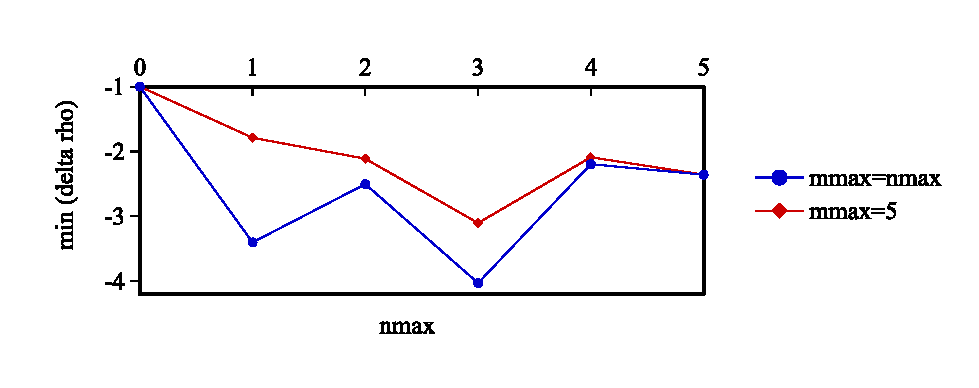
\includegraphics[bb=0bp 10bp 454bp 160bp,width=0.75\columnwidth]{_figure/results/min_delta_rho}
\par\end{centering}
\caption[The minimum value of $\Delta\rho(\mathbf{r},\mathbf{\Omega})/\rho_{0}$
after a forward-backward \acs{GSHT} process]{The minimum value of $\Delta\rho(\mathbf{r},\mathbf{\Omega})/\rho_{0}$
after a forward-backward \acs{GSHT} process with respect to $n_{\max}$.
Computed for a $45^{3}$ grid ($L=25$) for a converged density of
an artificial charged LJ center $\mathrm{CH}_{4}^{+0.4}$. \label{fig:unphysical-rho} }
\end{figure}

Theoretically, we expect this minimum value approach to zero when
increasing $m_{\max}$ or $n_{\max}$, which is not exactly the case.
That means perhaps the order of expansion is still far from to find
a tendency. Knowing that $\rho(\mathbf{r},\mathbf{\Omega})/\rho_{0}\rightarrow0$
at center of the solute and $\rho(\mathbf{r},\mathbf{\Omega})/\rho_{0}\rightarrow1$
far from the solute, the error can be said oblivious within the computing
capacity ($n_{\max}<5$), that means we cannot expand rightly the
density $\rho$ on \acs{GSH} projections, where. But this have a
much less effect on the functional gradient $\gamma$ that we evaluate,
because in a convolution product, $\Delta\hat{\rho}(\mathbf{k},\mathbf{\Omega})$
and the \acs{DCF} $\hat{c}(k,\mathbf{\Omega}_{1},\mathbf{\Omega}_{2})$
can be both expended, and product of higher order terms vanishes more
easily. Latter we will show that the profile of $\gamma$ and the
free energy $\mathcal{F}_{\mathrm{exc}}$ can already converge within
$n_{\max}<5$.

\section{Comparison between branches}

As shown in figure \ref{fig:Possible-algorithms}, if we fixe $\Delta\rho(\mathbf{r},\mathbf{\Omega})$
to a recombination of \acs{GSH} projections, all methods using the
same \acs{DCF} should give mathematically identical results. The
most direct comparison is the free energy evaluated during 1 iteration.
And to be more strict, is also interesting to compare the profile
of $\gamma$.

\subsection{Difference in energy evaluation}

As shown in table \ref{tab:free-energy}, the methods using the same
\acs{DCF} at the same $m_{\max}$ which is mathematically identical
in an infinite condition, give nearly the same results.

\begin{table}[H]
\begin{centering}
\begin{tabular*}{1\linewidth}{@{\extracolsep{\fill}}llll}
\toprule 
\tableheadline{Method} & $n_{\max}$ & \tableheadline{DCF} & \tableheadline{Free Energy} {\footnotesize{}(kJ/mol)}\tabularnewline
\midrule
\texttt{\textbf{\footnotesize{}dipole}} & {\footnotesize{}1} & {\footnotesize{}{[}ref mdft{]}} & {\footnotesize{}13.1915264499904339}\tabularnewline
\texttt{\textbf{\footnotesize{}naive\_dipole}} & {\footnotesize{}1} & {\footnotesize{}{[}ref mdft{]}} & {\footnotesize{}13.1915269013357985}\tabularnewline
\midrule 
\texttt{\textbf{\footnotesize{}naive\_nmax1}} & {\footnotesize{}1} & {\footnotesize{}\citep{puibasset_bridge_2012}{*}} & {\footnotesize{}18.6052247636086854}\tabularnewline
\texttt{\textbf{\footnotesize{}convolution\_standard}} & {\footnotesize{}1} & {\footnotesize{}\citep{puibasset_bridge_2012}{*}} & {\footnotesize{}18.6093390102806886}\tabularnewline
\midrule 
\texttt{\textbf{\footnotesize{}naive\_interpolation}} & {\footnotesize{}2} & {\footnotesize{}\citep{puibasset_bridge_2012}} & {\footnotesize{}26.8444355457069044}\tabularnewline
\texttt{\textbf{\footnotesize{}naive\_standard}} & {\footnotesize{}2} & {\footnotesize{}\citep{puibasset_bridge_2012}} & {\footnotesize{}26.9897310488084479}\tabularnewline
\texttt{\textbf{\footnotesize{}convolution\_standard}} & {\footnotesize{}2} & {\footnotesize{}\citep{puibasset_bridge_2012}} & {\footnotesize{}26.9163932581793155}\tabularnewline
\texttt{\textbf{\footnotesize{}convolution\_asymm}} & {\footnotesize{}2} & {\footnotesize{}\citep{puibasset_bridge_2012}} & {\footnotesize{}26.9163932581793155}\tabularnewline
\texttt{\textbf{\footnotesize{}convolution\_pure\_angular}} & {\footnotesize{}2} & {\footnotesize{}\citep{puibasset_bridge_2012}} & {\footnotesize{}26.9163932581793155}\tabularnewline
\bottomrule
\end{tabular*}
\par\end{centering}
\caption[Free energy calculated during 1 iteration]{Free energy calculated during 1 iteration for a $32^{3}$ grid ($L=20\textrm{Å}$)
for a fake LJ center $\mathrm{CH_{4}^{+0.33}}$, using a converged
density as input. Here $m_{\max}=n_{\max}$. \textcolor{red}{``{*}''
means ancient DCF, not so much difference.}\label{tab:free-energy}}
\end{table}
 

The light difference between \texttt{\textbf{naive\_nmax1}} and \texttt{\textbf{convolution\_standard}}
at $m_{\max}=1$ is due to the artificial decoration at $k$-border
showing in later section, and the difference between \texttt{\textbf{naive\_interpolation}}
and \texttt{\textbf{naive\_standard}} and \texttt{\textbf{convolution}}
methods are also acceptable, which is natural to be lightly different
due to the interpolation error and the \acs{GSH} expansion (the $\rho$
recombination of \acs{GSH} projections will be discussed later).
This supports by the way that we do not need the same order of \acs{GSH}
expansion for $\gamma$ than for $\Delta\rho$.

\subsection{A single k-kernel\label{subsec:A-single-k-kernel}}

Firstly, we are interested in the local paths from $\Delta\hat{\rho}_{\mu'\mu}^{m}(\mathbf{k})$
to $\hat{\gamma}_{\mu'\mu}^{m}(\mathbf{k})$ , that can be tested
independently for a certain $\mathbf{k}$. As shown in figure \ref{fig:k-kernel},
four algorithms are available to the purpose.

\begin{figure}[h]
\begin{centering}
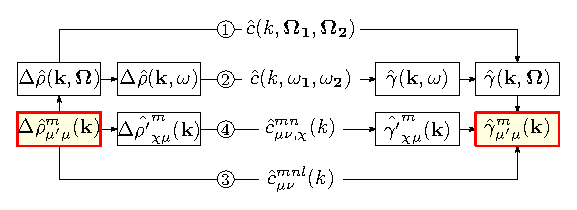
\includegraphics{_figure/algorithms_q}
\par\end{centering}
\caption{Schema of a k-kernel test \label{fig:k-kernel} }
\end{figure}

The program that compares each element of $\hat{\gamma}_{\mu'\mu}^{m}(\mathbf{k})$
issued from these 4 algorithms for a given $\Delta\hat{\rho}_{\mu'\mu}^{m}(\mathbf{k})$
is done by Mr. Luc Belloni, which shows that the $\hat{\gamma}_{\mu'\mu}^{m}(\mathbf{k})$
for the four algorithms are strictly identical. This means, the final
result of energy and structure is independent to the choice of path
inside a $k$-kernel, if $\Delta\hat{\rho}(\mathbf{k},\mathbf{\Omega})$
can be fully expended on \acs{GSH}s.

\subsection{k-border effect\label{subsec:k-border-effect}}

Here we test the whole process shown in figure \ref{fig:Possible-algorithms},
with $\Delta\rho(\mathbf{r},\mathbf{\Omega})$ generated from a recombination
of \acs{GSH} projections. Firstly, we compare the three \texttt{\textbf{convolution}}
algorithms passing by \acs{GSH} expansion. For a $64^{3}$ grid,
$n_{\max}=3$, the three algorithms \texttt{\textbf{convolution\_standard}},
\texttt{\textbf{convolution\_asymm}}, and \texttt{\textbf{convolution\_pure\_angular}}
gives the same free energy, but lightly different result when comparing
each element of $\gamma(\mathbf{r},\mathbf{\Omega})$, and this difference
seems to decrease when increase the number of grid points. More, the
projections $\gamma_{\mu'\mu}^{m}(\mathbf{r})$ which should be purely
real as explained in $\mathsection$\ref{subsec:Reduction-by-symmetry},
have a light imaginary part. But surprisingly, for a $65^{3}$ grid,
it gives numerically the same result for both the three algorithms
at machine precision.{*} \marginpar{{*} The detailed value of $\gamma$ which the paragraph of description
is based on haven't been noted, as it was regarded as a bug in the
code at that time, and the code had been then modified; and to redo
such a process takes a lot of time.}

The difference between these methods is found to be a special $k$-border
effect linking to even number grids.

As the symmetry
\begin{equation}
\Delta\hat{\rho'}_{\chi\mu}^{m}(\mathbf{k})=(-)^{m+\mu+\chi}\Delta\hat{\rho'}_{\chi,-\mu}^{m*}(-\mathbf{k})\label{eq:2-1}
\end{equation}
 is generated by two symmetries
\begin{equation}
\Delta\hat{\rho}_{\mu'\mu}^{m}(\mathbf{k})=(-)^{\mu'+\mu}\Delta\hat{\rho}_{-\mu',-\mu}^{m*}(-\mathbf{k})\label{eq:1-1}
\end{equation}
\begin{equation}
R_{\mu'\chi}^{m}(\hat{k})=(-)^{m+\mu'+\chi}R_{-\mu',\chi}^{m}(-\hat{k})\label{eq:3-1}
\end{equation}

For the points ``at border'', it's to say that after the FFT where
the point having $\pm k_{i}=k_{i}^{\mathrm{max}}$, $i=1,2,3$, for
example for $k_{1},$

\[
\Delta\hat{\rho}_{\mu'\mu}^{m}(\pm k_{1},k_{2},k_{3})=\Delta\hat{\rho}_{\mu'\mu}^{m}(k_{1}^{\mathrm{max}},k_{2},k_{3})
\]
is naturally put in the same array by FFT for the grids having even
number,\marginpar{For example, for a grid 1D, the FFT having 6 points gives the values
for indices 0,1,2,3,-2,-1, and the FFT having 7 points gives the values
for 0,1,2,3,-3,-2,-1.} as shown in figure \ref{fig:k-border-effect}. 

\begin{figure}[h]
\begin{centering}
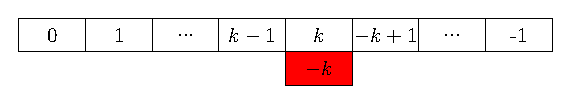
\includegraphics{_figure/k-border}
\par\end{centering}
\caption{$k$-border effect\label{fig:k-border-effect}}
\end{figure}

As \acs{FFT} possesses periodicity, the symmetry \ref{eq:1-1} can
always be respected at border. However, as
\begin{equation}
R_{-\mu',\chi}^{m}(-\hat{k}\equiv(-k_{1},-k_{2},-k_{3}))\neq R_{\mu',\chi}^{m}(k_{1}^{\mathrm{max}},-k_{2},-k_{3})
\end{equation}
the symmetries (\ref{eq:3-1}) and (\ref{eq:2-1}) are not respected
for these points. In the backward process, if we make sense of all
the $\gamma_{\mu'\mu}^{m}(\mathbf{k})$, as
\[
\gamma_{\mu'\mu}^{m}(-\hat{k}\equiv(-k_{1},-k_{2},-k_{3}))\neq\gamma_{\mu'\mu}^{m}(k_{1}^{\mathrm{max}},-k_{2},-k_{3})
\]
the symmetry
\begin{equation}
\gamma_{\mu'\mu}^{m}(\mathbf{k})=(-)^{\mu'+\mu}\gamma_{-\mu',-\mu}^{m*}(-\mathbf{k})\label{eq:1-1}
\end{equation}
is not respected totally, and this imposes that $\gamma_{\mu'\mu}^{m}(\mathbf{r})$
have a imaginary part. This imaginary part has been omitted implicitly
in the ``real to complex'' \acs{FFT} process of used in for example
\texttt{\textbf{convolution\_standard}}, for \acs{FGSHT}, or \texttt{\textbf{convolution\_pure\_angular}}
for FFT3D process. It is to say, we keep only the part of none-negative
$\mathbf{k}$ or none-negative $\mu$, supposing that the part we
omit respects the symmetry.

The right way to treat this issue is to artificially impose at the
border:
\begin{equation}
R_{\mu',\chi}^{m}(k_{i}^{\mathrm{max}})=\frac{1}{2}\left[R_{\mu',\chi}^{m}(k_{i})+R_{\mu',\chi}^{m}(-k_{i})\right]
\end{equation}
where $i$ is the conflict index in figure \ref{fig:k-border-effect}.
If more than one dimensions are in conflict, this process can be done
twice (4 terms for ``edges'' of the cube) or three times (8 terms
for ``vertices''). The point $\mathbf{k}=\hat{0}$ is different,
as it was define along $z$ axes to avoid implementation crash, it
doesn't respect eq. (\ref{eq:3-1}) and (\ref{eq:2-1}) neither. But
this point compared to hundreds thousands of total points is negligible.

The energies given by \texttt{\textbf{naive\_standard}} and the \texttt{\textbf{convolution}}
algorithms are identical for a $65^{3}$ and $n_{\max}=3$ grid, but
the element of $\gamma(\mathbf{r},\mathbf{\Omega})$ have a mysterious
difference at order of $10^{-2}$, seemed to be aleatory. A test redone
for a $45^{3}$ grid is shown in figure \ref{fig:Difference-in-gamma}.

\begin{figure}[H]
\begin{centering}
\subfloat[$\delta\hat{\gamma}(\mathbf{k},\mathbf{\Omega})$]{\begin{centering}
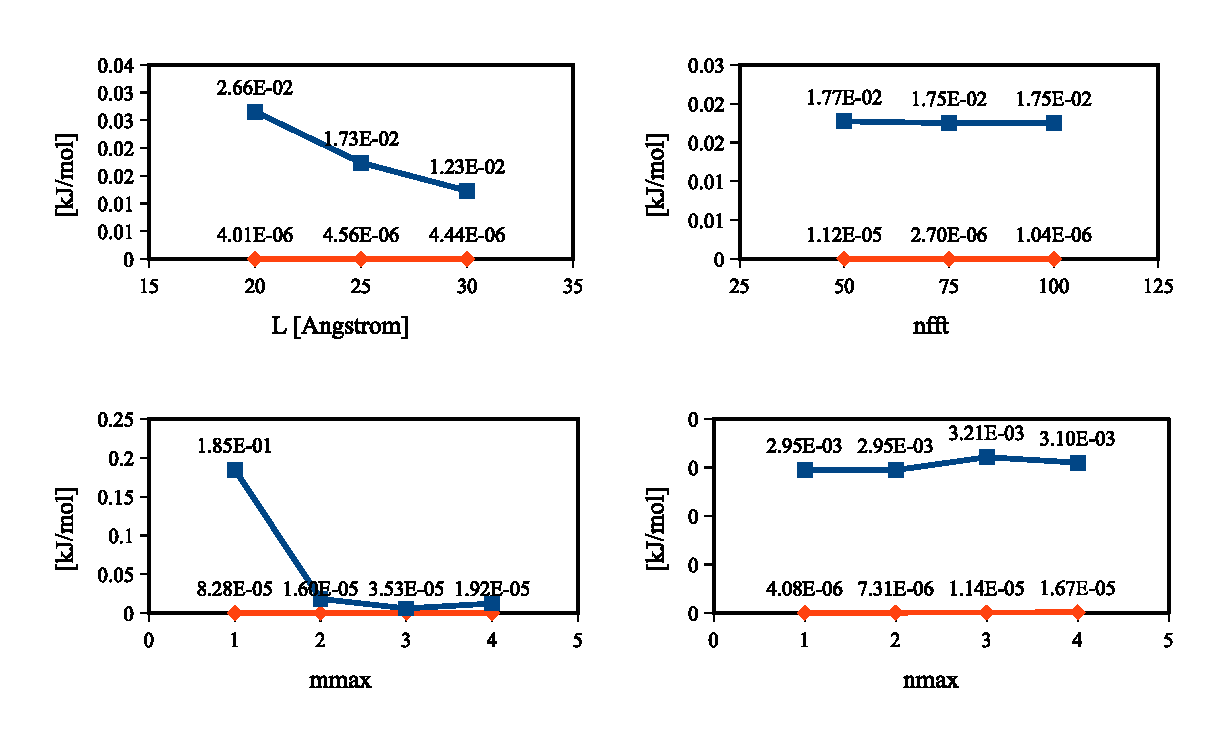
\includegraphics[width=0.75\columnwidth]{_figure/results/diff_k_gamma}
\par\end{centering}

}
\par\end{centering}
\begin{centering}
\subfloat[$\delta\gamma(\mathbf{r},\mathbf{\Omega})$]{\begin{centering}
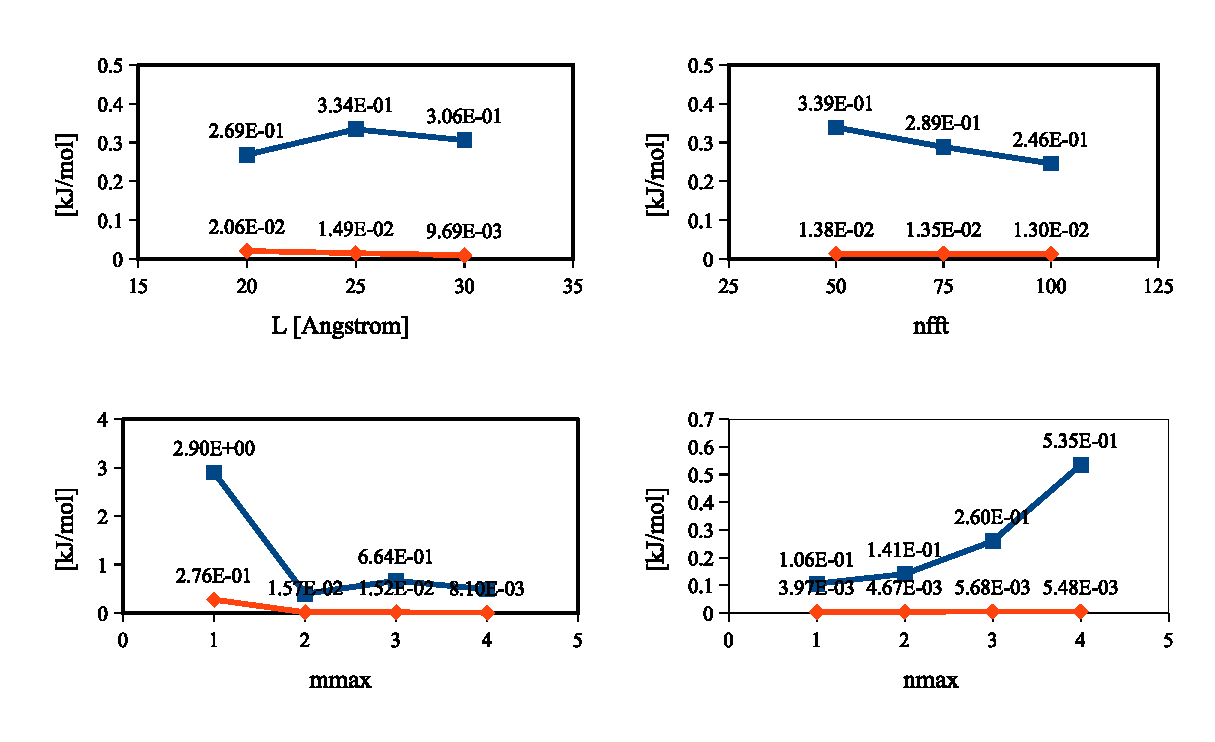
\includegraphics[width=0.75\columnwidth]{_figure/results/diff_gamma}
\par\end{centering}
}
\par\end{centering}
\caption[Maximum and average difference in $\hat{\gamma}(\mathbf{k},\mathbf{\Omega})$
and $\gamma(\mathbf{r},\mathbf{\Omega})$]{Maximum and average difference in $\hat{\gamma}(\mathbf{k},\mathbf{\Omega})$
and $\gamma(\mathbf{r},\mathbf{\Omega})$, for tests of different
box length$L$, different number of grid nfft in one dimension, $n_{\max}=1,4$
for $m_{\max}=n_{\max}$, and $n_{\max}=1,4$ for $m_{\max}=5$.\label{fig:Difference-in-gamma}}
\end{figure}

We can conclude very rudely that this error depends on the angular
quadrature $m_{\max}$. The dependence is natural, as the difference
between algorithms \texttt{\textbf{naive}} and \texttt{\textbf{convolution}}
is the treatment of the angular part. There is also a dependence on
$L$ in the $k$-space, but after \acs{FFT} it is mixed. The augmentation
of error in the $n_{\max}$ chart is unnatural, implying there is
perhaps a still bug in the code.

In a word, this mysterious difference cannot be yet explained, as
the \texttt{\textbf{naive}} methods does not have the $k$-border
effect linked to symmetry, on the other hand we used a odd grid, we
could not yet distinguish that it is a bug in the implementation,
in the test or in the theory. The projections $\gamma_{\mu\nu}^{mnl}(r)$
of this two algorithms seems to be identical (figure \ref{fig:gamma-proj}),
it is to say, the global structure of this two algorithms are almost
the same, and the error would not be very decisive.

\begin{figure}[h]
\begin{centering}
\includegraphics[width=0.65\columnwidth]{_figure/results/gamma_proj}
\par\end{centering}
\caption{A selection of rotational invariant projections $\gamma_{\mu\nu}^{mnl}(r)$
for a $65^{3}$ grid\label{fig:gamma-proj}}
\end{figure}


\section{Intrinsic variation of free energy\label{sec:Intrinsic-variation-of}}

Before study of free energy dependence on angular algorithms, we are
interested in the grid dependance, with can have an influence to the
tests later.

\begin{figure}[H]
\begin{centering}
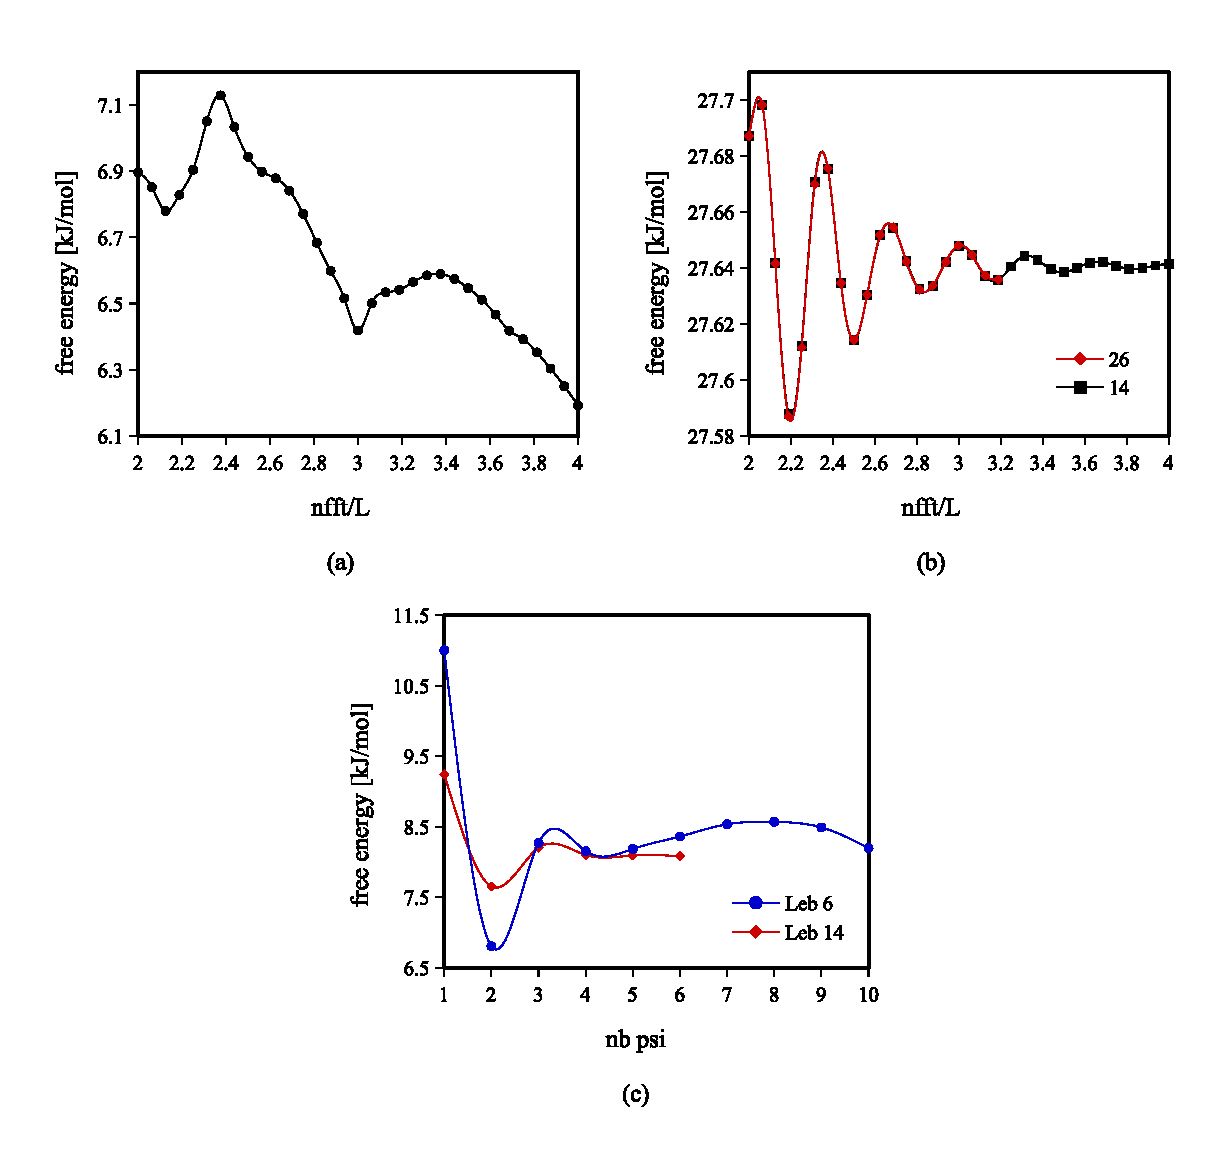
\includegraphics[bb=0bp 20bp 567bp 519bp,width=0.75\columnwidth]{_figure/results/grid_reso}
\par\end{centering}
\caption[Space-grid and $\Psi$ dependence of code MDFT]{Space-grid and $\Psi$ dependence of code MDFT. $L=32$. (a) $\mathrm{CH_{4}^{+0.33}}$
using dipole DCF with $m_{\max}=1$; (b) $\mathrm{CH_{4}}$ using
DCF of $m_{\max}=5$, Lebedev quadrature of order 1 and 2; (c) acetone
using dipole DCF and Lebedev quadrature, varying $\Psi$, nfft=128.
\label{fig:Space-grid-and-psi-dependence}}
\end{figure}

As shown in figure \ref{fig:Space-grid-and-psi-dependence} (a) and
(b), there is a dependence of calculated free energy on the space
grid resolution. for a charged solute, the energy has tendency to
decrease when increasing the resolution of grid (nfft). And this decrease
does not link to the border correction mentioned in $\mathsection$\ref{chpt:thermodynamic-quantities},
as the box length and the charge remain the same for the whole set
of test. From (b) we consider that at least 3 points grid in one dimension
per Angstrom is needed to reduce the uncertainty due to grid resolution.
Figure (c) fixed the Lebedev quadrature for $\Theta$ and $\Phi$,
but leaved varying the $\Psi$. We can also see a dependence on $\Psi$.
which does not vanish when increasing the resolution of grid. As during
the whole thesis the $\Psi$ is theoretically fixed in the same order
with $\Theta$ and $\Phi$, this remains an issue for further verification.
We can roughly conclude that an error around 1 kJ/mol is common for
this code.

\section{Series of charged LJ centre}

To valid the method, we chose a series of LJ centre, which possess
the LJ parameters of $\mathrm{C}\mathrm{H}_{4}$ in \textcolor{red}{{[}ref{]}},
and have a various charge from -1.0 to 1.0 (table \ref{tab:Parameters-of-charged-met}).\marginpar{For both IET, and DM results, 298K is used according to habitude instead
of 303K recommended in reference \citep{SPC/E}. For MDFT, 300K and
298K are used.}

\begin{table}[h]
\begin{centering}
\begin{tabular*}{1\linewidth}{@{\extracolsep{\fill}}lllllll}
\toprule 
\tableheadline{Charge} & $\sigma$ {[}$\textrm{Å}${]} & $\epsilon$ {[}$\mathrm{kJ\cdot mol^{-1}}${]} & $x$ {[}$\textrm{\AA}${]} & $y$  {[}$\textrm{\AA}${]} & $z$ {[}$\textrm{\AA}${]} & \tableheadline{Number Density} {[}$\lyxmathsym{\AA}^{-3}${]}\tabularnewline
\midrule
-1.0 to 1.0 & 3.73  & 1.23  & 0 & 0 & 0 & 0.0332891 \textcolor{red}{{[}ref,temperature{]}}\tabularnewline
\bottomrule
\end{tabular*}
\par\end{centering}
\caption{Parameters of charged Lenard-Jones centre (modified from $\mathrm{C}\mathrm{H}_{4}$)
\label{tab:Parameters-of-charged-met}}
\end{table}


\subsection{Box length dependance and charge dependance of free energy}

As discussed in section \ref{chpt:thermodynamic-quantities}, for
single ions, two types of corrections need to be added on the free
energy, which depend on the box length and and charge of the ion.
To verify these dependence, we implement a systematic calculation
from charge, using 3 different methods, where the parameters are shown
in table \ref{tab:parameters-ch4}. It should be noted that, the \texttt{\textbf{naive\_interpolation}}
only used 14 Lebedev and 3 $\Psi$ angles to converge, which gives
exactly the same result with 26 Lebedev and 4 $\Psi$ angles, that
means, the \texttt{\textbf{naive}} methods do not need an order of
quadrature $m_{\max}$ to be greater than the order of DCF $n_{\max}$.
The -1 side has problem of convergence, and all the converged results
are presented.

\begin{table}[h]
\begin{centering}
\begin{tabular*}{1\linewidth}{@{\extracolsep{\fill}}llll}
\toprule 
\tableheadline{Method} & nfft/$L$ & $m_{\max}$ & $n_{\max}$\tabularnewline
\midrule
\texttt{\textbf{naive\_nmax1}} & 3 & 1 & 1\tabularnewline
\texttt{\textbf{naive\_interpolation}} & 3 & 2 (Leb) & 5\tabularnewline
\texttt{\textbf{convolution\_standard}} & 3 & 1 & 1\tabularnewline
\bottomrule
\end{tabular*}
\par\end{centering}
\caption{Methods and parameters for $\mathrm{C}\mathrm{H}_{4}$ series test.
{*} Leb is Lebedev quadrature, with is mathematically equivalent with
Gauss-Legendre quadrature but only ˜2/3 angles.\label{tab:parameters-ch4}}
\end{table}

The direct results collection are shown in figure \ref{fig:ch4_nmax1_lmn},
\ref{fig:ch4_nmax5_inter} and \ref{fig:ch4_nmax1_new} at the end
of this section. We can see that the dependence of box length for
each charge is almost linear, except the charge between $\left[-0.2,0.2\right]$.
This means, the influence of box length is much greater than the intrinsic
variation of result that mentioned in \ref{sec:Intrinsic-variation-of}.
The charge dependency is traced in figure \ref{fig:Quadratic-charge-dependence},
using all the number of slopes with respect to the square of their
charge ($q^{2}$). A linear regression is done to give the slope 1937.8
$\mathrm{kJ}\cdot\mathrm{mol^{-1}}\cdot\textrm{Å}$. This slope correspond
to the correction of type-B (normalized to give the right unity):
\begin{equation}
\dfrac{\xi}{2}\left(1-\dfrac{1}{\varepsilon}\right)=1943.2\,\mathrm{kJ}\cdot\mathrm{mol^{-1}}\cdot\textrm{Å}
\end{equation}

\begin{figure}[H]
\begin{centering}
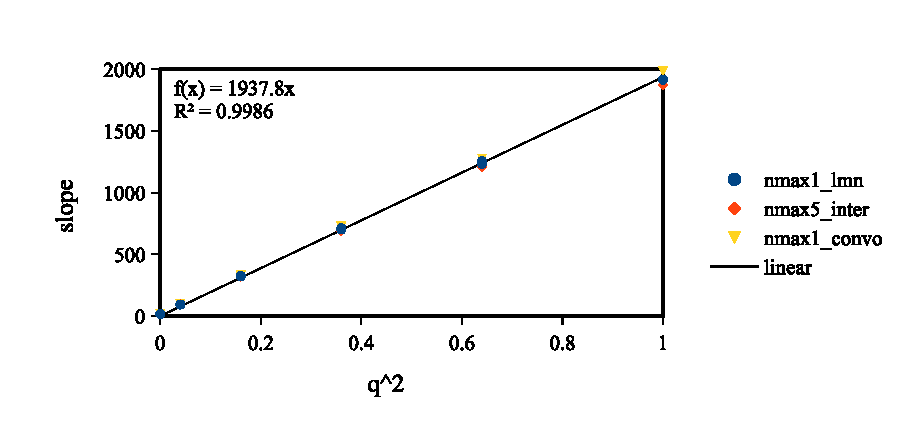
\includegraphics[bb=0bp 20bp 425bp 178bp,scale=0.6]{_figure/results/ch4_slope}
\par\end{centering}
\caption{Quadratic charge dependence of free energy of $\mathrm{C}\mathrm{H}_{4}$
centre series\label{fig:Quadratic-charge-dependence}}
\end{figure}
The intercept values in each of figure \ref{fig:ch4_nmax1_lmn} to
\ref{fig:ch4_nmax1_new} correspond to the free energy of an infinite
box. The \acs{IET} results are done with $R_{\max}=102.4\textrm{Å}$,
and need a correction of $-2.556k_{\mathrm{B}}T$. \textcolor{red}{(need
more details.)} The differences in free energy between MDFT and IET
are given in figure \ref{fig:Comparison-to-IET,without-correction}.
The linear regression is done with all existing points in this figure.
The slope 87.653 $\mathrm{kJ}\cdot\mathrm{mol^{-1}}$ corresponds
to the correction of type-C (normalized to give the right unity):
\begin{equation}
\eta\gamma=82.104\mathrm{kJ}\cdot\mathrm{mol^{-1}}\label{eq:eta-gamma}
\end{equation}
These two numbers are a little different, principally due to a lack
of point at the -1 side.

\begin{figure}[h]
\begin{centering}
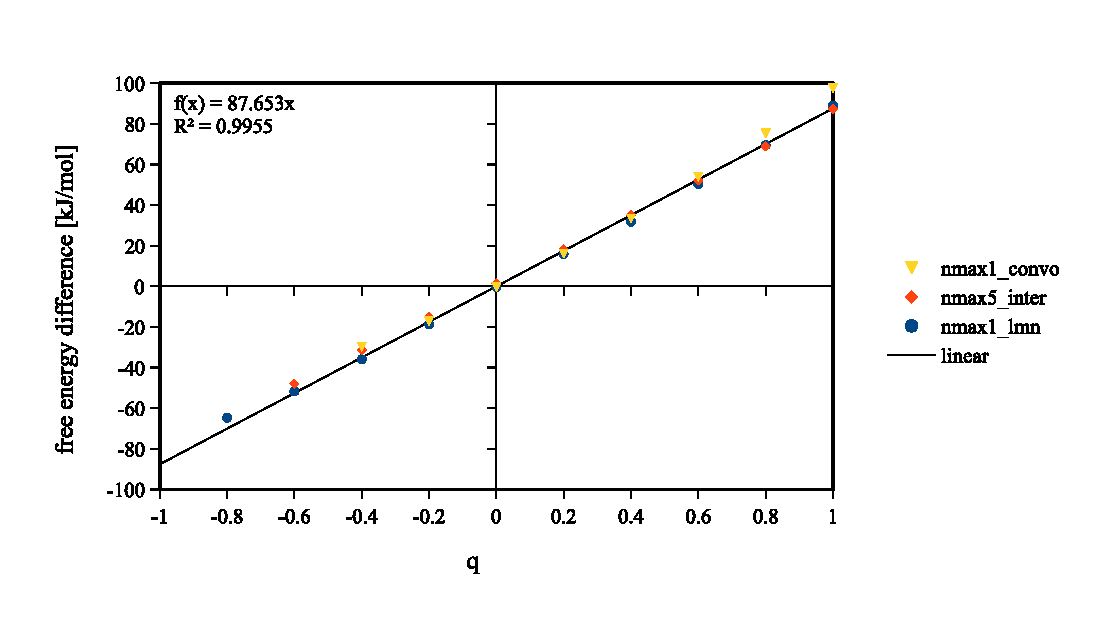
\includegraphics[bb=0bp 20bp 510bp 263bp,scale=0.6]{_figure/results/ch4_diff_energy}
\par\end{centering}
\caption{Comparison to IET, without P-scheme correction\label{fig:Comparison-to-IET,without-correction}}
\end{figure}


\subsection{Comparison with IET after corrections}

The figure \ref{fig:Comparison-to-IET,without-correction} after correction
with eq. (\ref{eq:eta-gamma}) gives figure \ref{fig:Comparison-to-IET,with-corr}.
It is shown that they are not perfectly agreed with each other. The
$n_{\max}=1$ methods have large difference when the charge increased,
especially the \texttt{\textbf{convolution\_standard}} using GSH expansion.
Knowing that during 1 iteration, the \texttt{\textbf{naive\_nmax1}}
and the \texttt{\textbf{convolution\_standard}} only give a slight
difference in free energy (table \ref{tab:free-energy}). The $n_{\max}=5$
have an energy shift about 2 $\mathrm{kJ}\cdot\mathrm{mol^{-1}}$,
which cannot have an explanation. but overall, to have 2 $\mathrm{kJ}\cdot\mathrm{mol^{-1}}$
per 100 $\mathrm{kJ}\cdot\mathrm{mol^{-1}}$ is already a good result.

\begin{figure}[H]
\begin{centering}
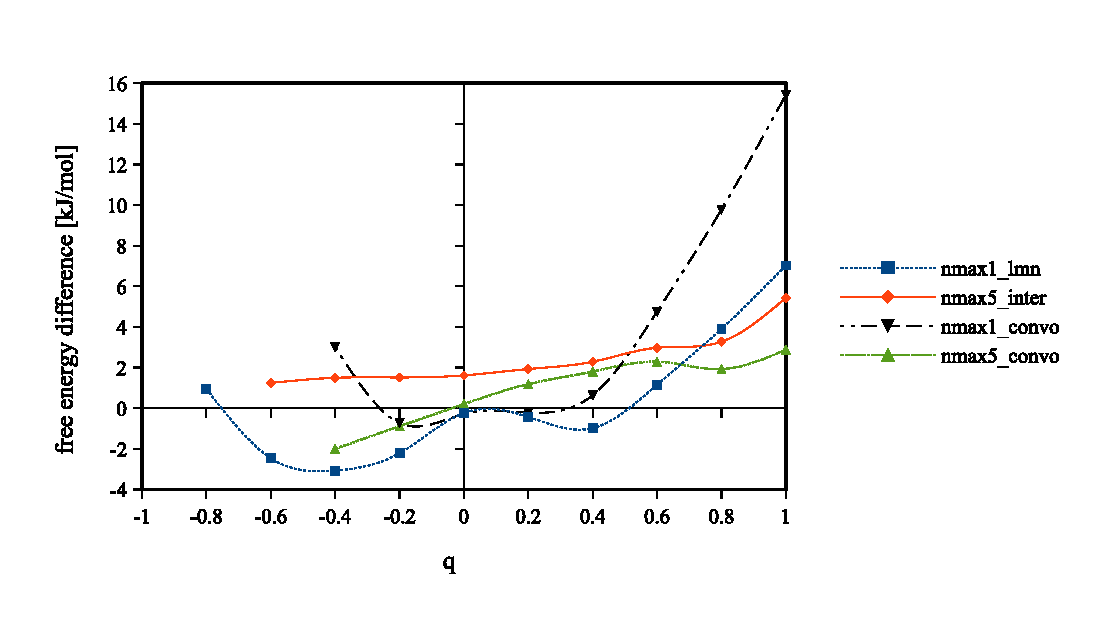
\includegraphics[bb=0bp 20bp 510bp 263bp,scale=0.6]{_figure/results/ch4_diff_inter}
\par\end{centering}
\caption{Comparison to IET, with P-scheme correction\label{fig:Comparison-to-IET,with-corr}}
\end{figure}

The case of $m_{\max}=5$ , $n_{\max}=0,\ldots,5$ with \texttt{\textbf{convolution\_standard}}
is shown in figure \ref{fig:Comparison-to-IET,nmax0-5}. It is interesting
to see how energy evaluate with $n_{\max}$ while fixing $m_{\max}$.
As we said, $\gamma$ is more smooth than $\rho$, that means we can
have $n_{\max}<m_{\max}$ to economize computing cost. Results shows
that within $n_{\max}\geq3$ for $n_{\max}=5$, the error is acceptable.
But again, the dependence on $q$ after correction is in incomprehensible.
And compared to \texttt{\textbf{naive\_interpolation}} in figure \ref{fig:Comparison-to-IET,with-corr},
we see that these error for $n_{\max}=5$ is different.

\begin{figure}[H]
\begin{centering}
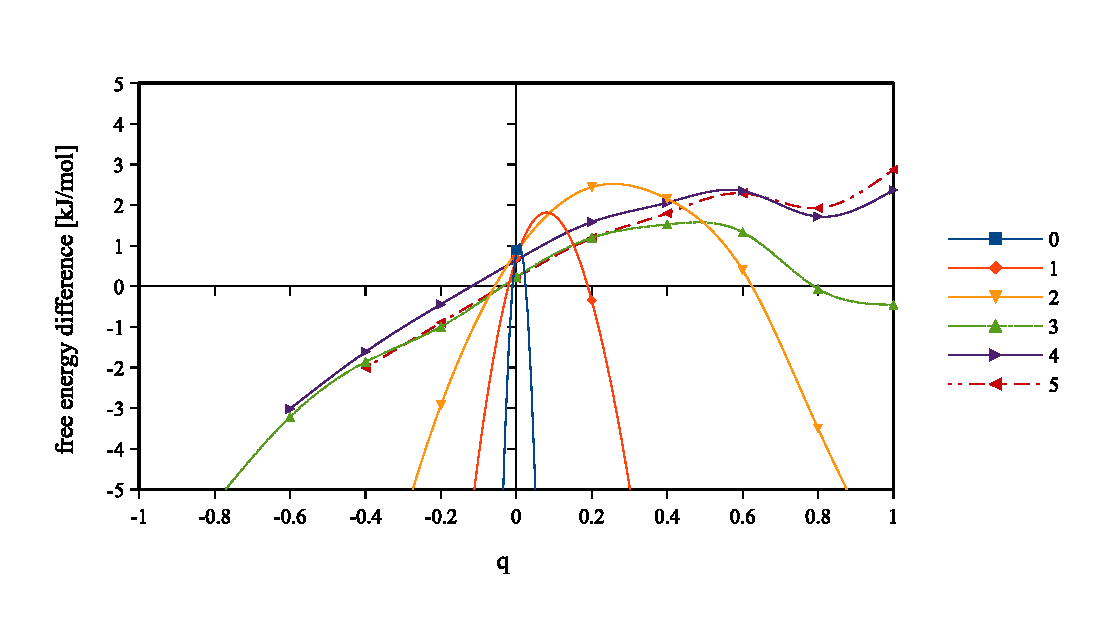
\includegraphics[bb=0bp 20bp 510bp 263bp,scale=0.6]{_figure/results/ch4_diff_mmax5}
\par\end{centering}
\caption{Comparison to IET, with P-scheme correction, $m_{\max}=5$ , $n_{\max}=0,\ldots,5$
\label{fig:Comparison-to-IET,nmax0-5}}
\end{figure}

The profile of $\rho$ can expended on rotational invariants which
is discussed in $\mathsection$\ref{chpt:solvation-structure}. The
comparison with IET is done for three charges, 0, -0.6 and +1. Shown
in figure \ref{fig:Comparison-to-IET.rot_invar}. Watch that the 0
and -1 one of $m_{\max}=5$ corresponds well the result of IEM, but
the -0.6 one have a lot of noise. (In fact, this configuration had
difficulty to converge, and the given energy is not good, thus it
is deleted in figure \ref{fig:Comparison-to-IET,nmax0-5}.) The the
profiles of go much better $m_{\max}=2,3$. Normally, more points
means more precision. It may means that with $m_{\max}=5$ , there
is perhaps a bug of integer overflow that prevent the convergence
for high charges.

\begin{figure}[H]
\begin{centering}
\includegraphics[width=1\columnwidth]{/Users/Hostiphre/Desktop/_M1102/_figure/results/ch4_iet_struct}
\par\end{centering}
\caption{Comparison to IET. Profile of $\rho$ in rotational invariant projections,
L=24, nfft=72.\label{fig:Comparison-to-IET.rot_invar}}
\end{figure}


\subsection{Comparison with MD}

The comparison of RDF with MD results are shown in figure \ref{fig:Comparison-to-MD}.
We can see that for negative charges, there are a lot of shifts.

Discussion...

\begin{figure}[H]
\begin{centering}
\includegraphics[width=1\columnwidth]{/Users/Hostiphre/Desktop/_M1102/_figure/results/ch4_md}
\par\end{centering}
\caption{Comparison to IET. Profile of $\rho$ in rotational invariant projections.\label{fig:Comparison-to-MD}}
\end{figure}


\section{Premier conclusion}

From the results, we see that MDFT ... ``capable'' to produce the
same result with IEM for single ions. (but have more ability to calculate
3D molecules which is not suitable for spherical coordinates...)

\texttt{\textbf{naive\_interpolation}} is more stable compared to
\texttt{\textbf{convolution}} methods and can use less angles for
convergence, although in the computing time it cannot compare with
\texttt{\textbf{convolution}} methods, which will be discussed later.

\begin{figure}[h]
\begin{centering}
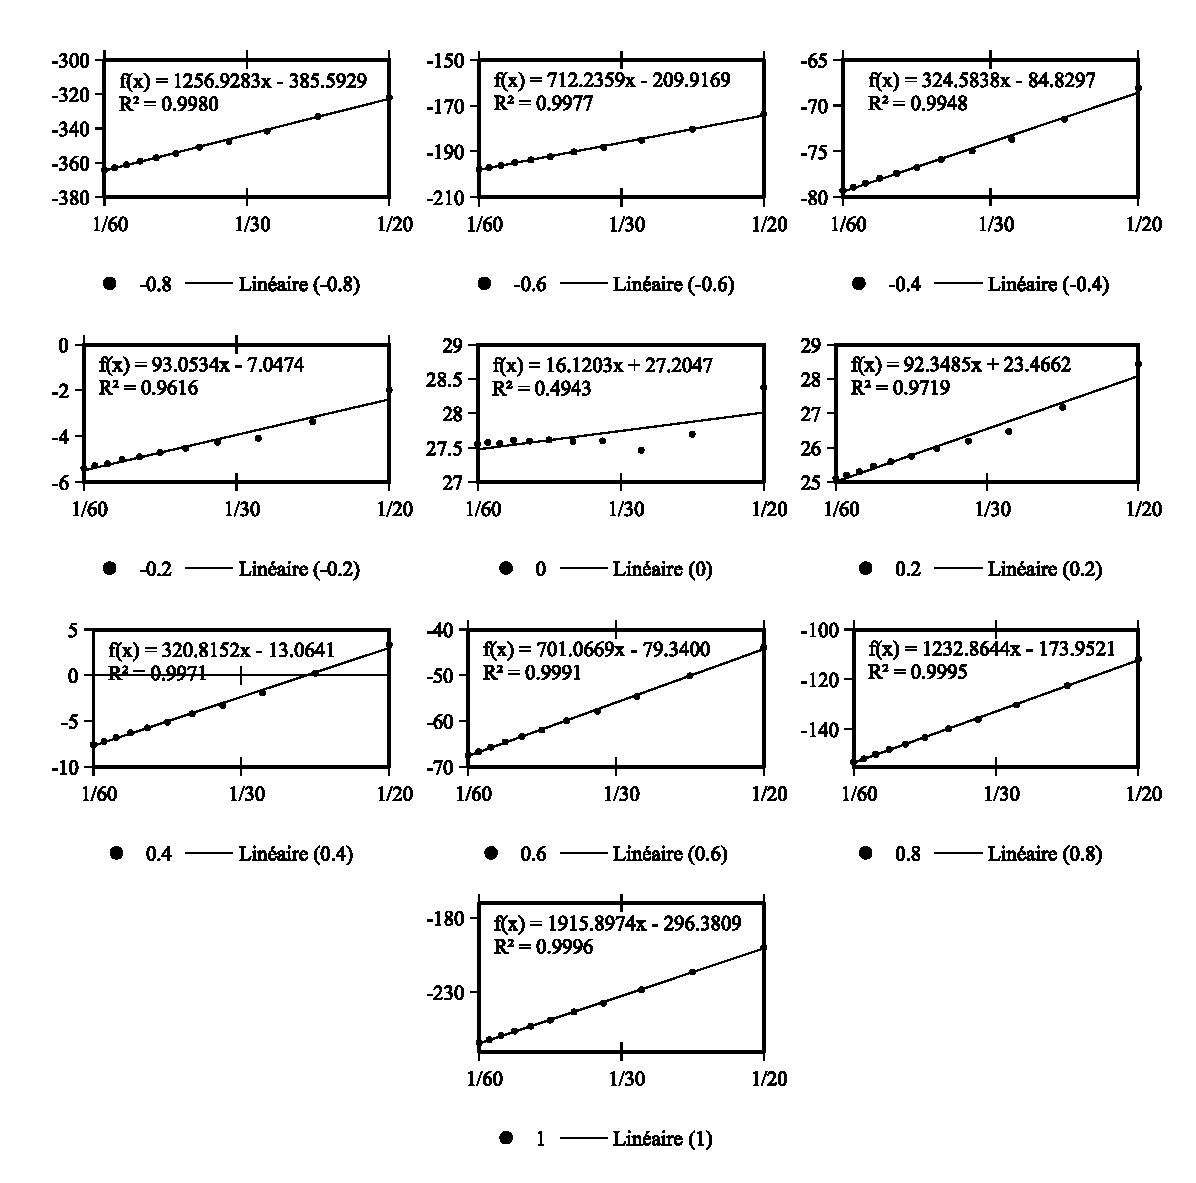
\includegraphics[width=0.95\columnwidth]{_figure/results/ch4_nmax1_lmn}
\par\end{centering}
\caption{Free energy (without correction) of charged $\mathrm{C}\mathrm{H}_{4}$
centre (-1.0 to 1.0) with respect to the box length, for \texttt{\textbf{naive\_nmax1}}
method, with $m_{\max}=n_{\max}=1$, at 300K.\label{fig:ch4_nmax1_lmn}}
\end{figure}

\begin{figure}[!th]
\begin{centering}
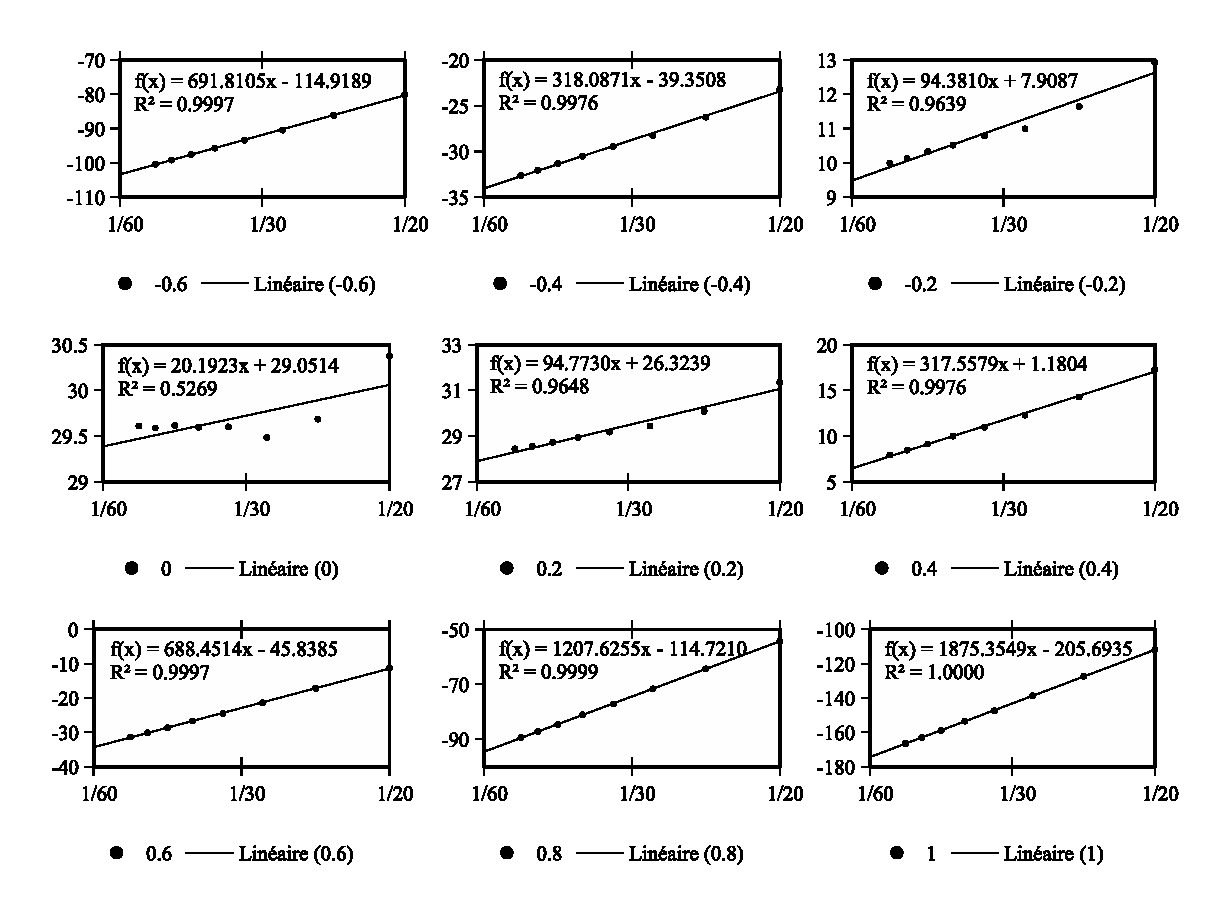
\includegraphics[width=0.95\columnwidth]{_figure/results/ch4_nmax5_inter}
\par\end{centering}
\caption{Free energy (without correction) of charged $\mathrm{C}\mathrm{H}_{4}$
centre (-1.0 to 1.0) with respect to the box length, for \texttt{\textbf{naive\_interpolation}}
method, with 14 angles of Lebedev quadrature angles for $\Theta$
and $\Phi$, 3 for $\Psi$, DCF of $n_{\max}=5$, at 300K.\label{fig:ch4_nmax5_inter}}
\end{figure}

\begin{figure}[!bh]
\begin{centering}
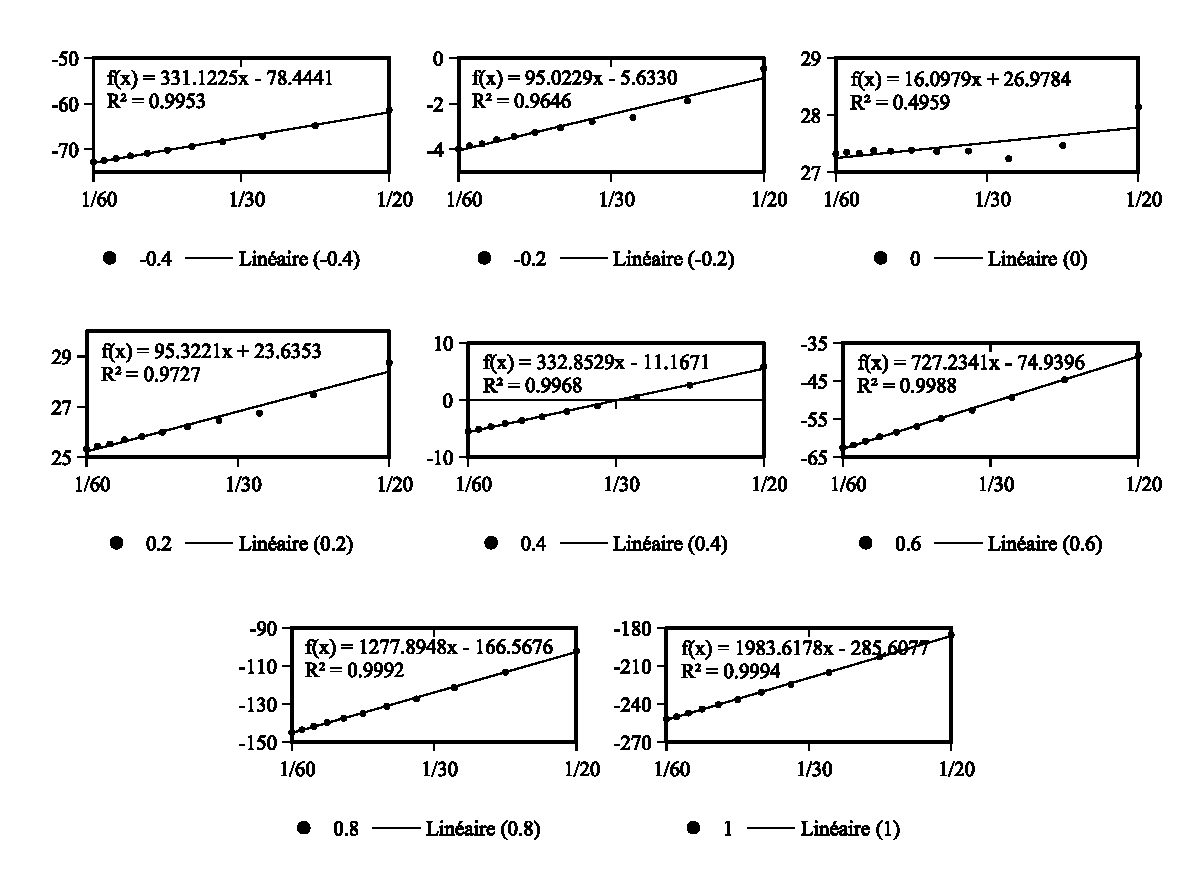
\includegraphics[width=0.95\columnwidth]{_figure/results/ch4_nmax1_new}
\par\end{centering}
\caption{Free energy (without correction) of charged $\mathrm{C}\mathrm{H}_{4}$
centre (-1.0 to 1.0) with respect to the box length, for \texttt{\textbf{convolution\_standard}}
method, with $m_{\max}=n_{\max}=1$, at 298.15K.\label{fig:ch4_nmax1_new}}
\end{figure}




\chapter{Computing Performance \label{chpt:seq-code-performance}}

This section evaluates the computing performance (timing) of the code.
Our goal is to show that the new algorithm of angular convolution
is much faster than the old naive one; the huge amount of simulation
during this thesis has proven that to be the case. But a raw result,
where the implementation goes for an indefinite number of iterations
during minimization, cannot give a proper and systematic performance
evaluation. This is the purpose of this section.

In this section, we will evaluate the performance only within the
$\mathcal{F}_{\mathrm{exc}}$ term, knowing that other two terms takes
time of the same magnitude than the new algorithms for $\mathcal{F}_{\mathrm{exc}}$
part. The spatial and angular grid dependence of branches are discussed.

\section{FFT}

The \acs{FFT} play an important role in the implementation, which
is used by the spatial convolution and the \acs{FGSHT} process. 

\begin{figure}[H]
\begin{centering}
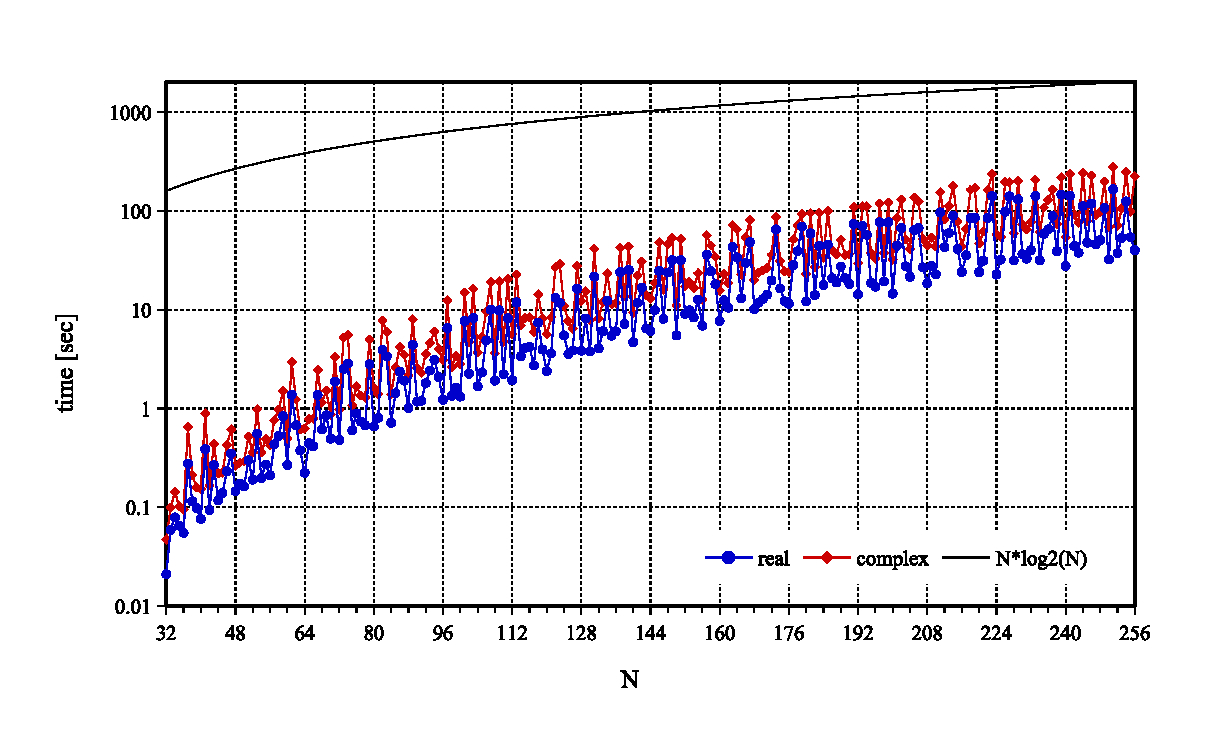
\includegraphics[bb=0bp 20bp 567bp 310bp,width=1\columnwidth]{_figure/results/fftw_timing}
\par\end{centering}
\caption{Timing of \acs{FFT} for real-to-complex and complex-to-complex processes
with respect to grid number $N$\label{fig:timing-FFT}}
\end{figure}

Referring to figure \ref{fig:timing-FFT}, the dependance on $O(N\log_{2}N)$
\citep{Numerical_Recipes_3ed} doesn't totally exist, but of the same
form, depending on the algorithm of \acs{FFT} \citep{Briggs-DFT}.
It should be noted that a grid of prime number is always at the peaks
in the figure, which means it can be 2 or more times longer than that
of the composite number around. Therefore it is better to use an even
number grid, where the $k$-border correction in $\mathsection$\ref{subsec:k-border-effect}
is absolutely involved in. Apart from this conclusion, to compare
between the algorithms for angular part involved in this thesis, we
are not really interested in computing performance with respect to
the number of spatial grid. However, the ratio of real and complex
\acs{FFT} timing is important, illustrated in figure \ref{fig:fft-real-to-complex},
where the ratio between real-to-complex and complex-to-complex \acs{FFT}
processes is 0.54, near the theoretical ratio 0.5. For example, we
process $n_{\mathrm{angle}}$ real to complex \acs{FFT}, then $n_{\mathrm{spatial}}/2$
complex to complex \acs{FGSHT}. Or we process $n_{\mathrm{spatial}}$
real to complex \acs{FGSHT}, then $n_{\mathrm{proj}}/2$ complex
to complex \acs{FFT}. This should not give a great difference if
$n_{\mathrm{angle}}\sim n_{\mathrm{proj}}$ for small $n_{\max}$.
If the the ratio is not 1:2, it will have an influence on the choice
of algorithm.
\begin{center}
\begin{figure}[h]
\begin{centering}
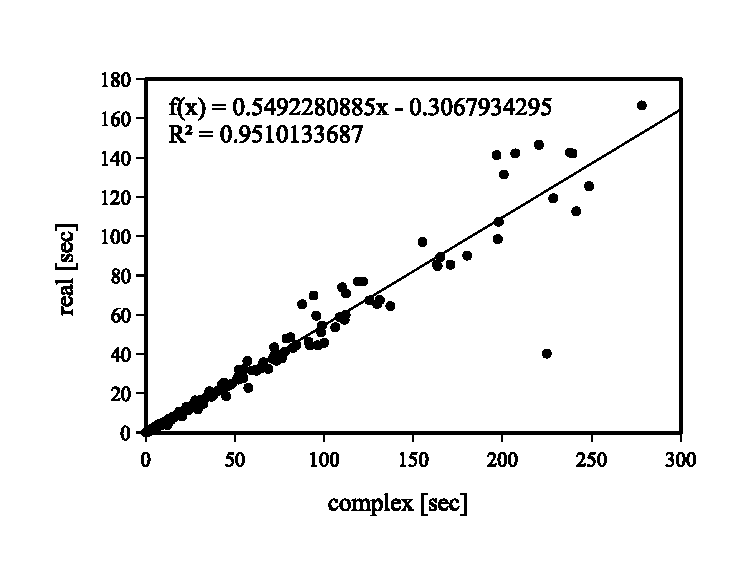
\includegraphics[bb=0bp 20bp 340bp 235bp,width=0.5\columnwidth]{_figure/results/fftw_real_v_cmplx}
\par\end{centering}
\caption{Timing of real-to-complex \acs{FFT} processes with respect to its
complex-to-complex process of the same grid number $N$\label{fig:fft-real-to-complex}}
\end{figure}
\par\end{center}

\section{FGSHT}

The computing times of \acs{GSHT} and \acs{FGSHT} are shown in figure
\ref{fig:time-gsht-fgsht}. There is no reason to see in detail how
much \acs{FFT} has accelerated the \acs{GSHT} process, but clearly
\acs{FGSHT} can be 100 times faster than \acs{GSHT}, and \acs{GSHT}
for the symmetry of $\Psi$, $s=1$ is on average 5 times longer than
$s=2$ ($s$ being the \acs{MRSO} defined in $\mathsection$\ref{sec:fgsht}).
As accuracy test shows that \acs{GSHT} and \acs{FGSHT} give exactly
the same result, and the case $m_{\max}<n_{\max}$ is never needed,
it is possible to utilize \acs{FGSHT} in all the cases to have a
faster performance.
\begin{center}
\begin{figure}[H]
\begin{centering}
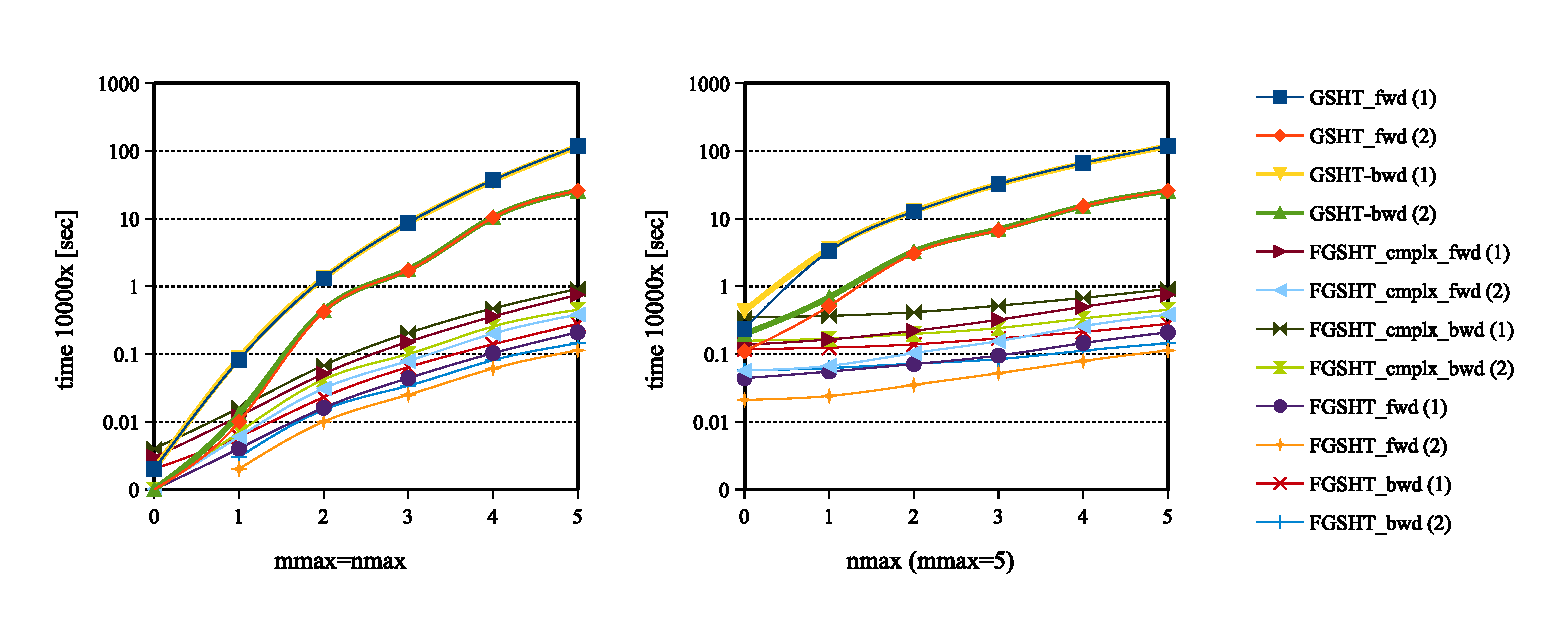
\includegraphics[bb=0bp 20bp 731bp 263bp,width=1\columnwidth]{_figure/results/fgsht_perf}
\par\end{centering}
\caption[Computing time of \acs{GSHT} and \acs{FGSHT}]{Computing time of \acs{GSHT} and \acs{FGSHT} (per 10000 times),
between parentheses is the order of symmetry axes $s$\label{fig:time-gsht-fgsht}}
\end{figure}
\par\end{center}

However, it is important to know the ratio between real and complex
\acs{FGSHT} processes for the same reason as \acs{FFT}. It is demonstrated
that this number is 0.3 in all cases, and it does not depend on $m_{\max}$,
$n_{\max}$ or $s.$ The difference between these two is that the
real one performs real-to-complex \acs{FFT} for the $\Phi,\Psi$
grid and calculates only slightly more than half of projections ($\mu\geq0$)
than the complex one.\textcolor{red}{{} }Theoretically, the ratio should
be greater than 0.5. This could mean there may be an extra process
in the complex one, or it is controlled by the memory. Ultimately,
the final result 0.3 means, that doing $n_{\mathrm{spatial}}$ real
to complex \acs{FGSHT} takes only 0.6 the time of doing $n_{\mathrm{spatial}}/2$
complex to complex \acs{FGSHT}, which means in \texttt{\textbf{convolution\_standard}}
we use less time to compute \acs{FGSHT} than in \texttt{\textbf{convolution\_pure\_angular}}.
\textcolor{red}{(Which is in fact not observed in the following tests.)}
\begin{center}
\begin{figure}[H]
\begin{centering}
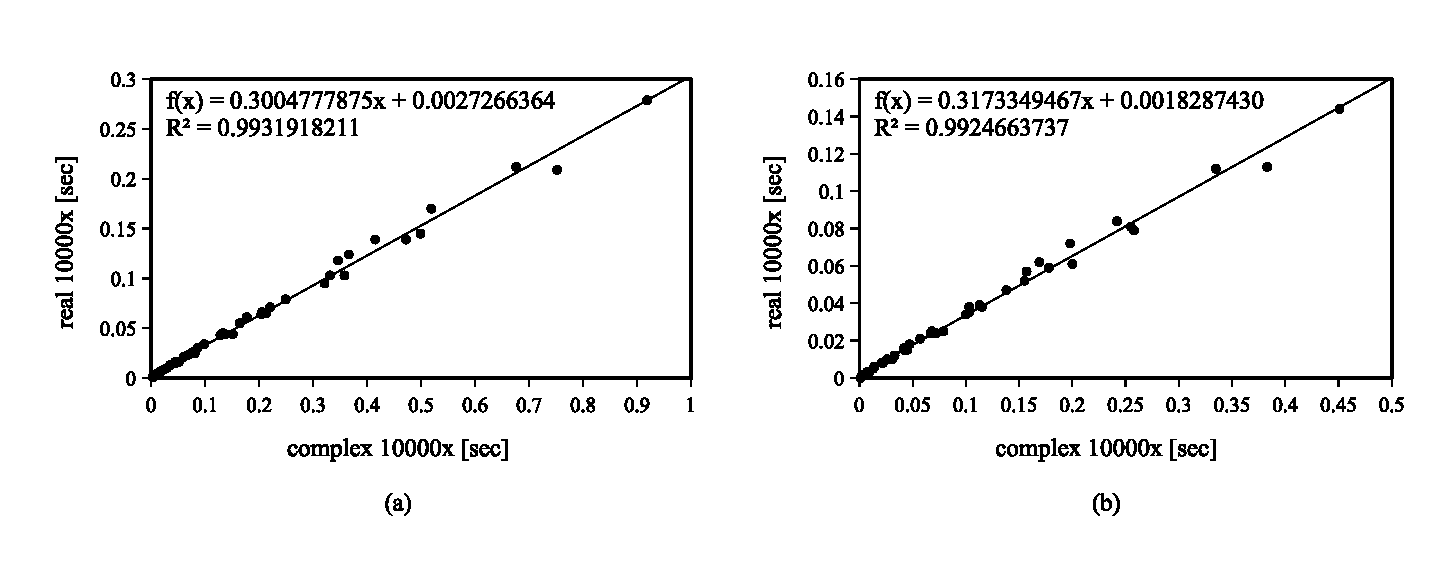
\includegraphics[bb=0bp 20bp 680bp 235bp,width=1\columnwidth]{_figure/results/fgsht_real_v_cmplx}
\par\end{centering}
\caption[Timing of real-to-complex \acs{FGSHT} processes with respect to its
complex-to-complex process of the same $m_{\max}$ and $n_{\max}$]{Timing of real-to-complex \acs{FGSHT} processes with respect to
its complex-to-complex process of the same $m_{\max}$ and $n_{\max}$,
for $s=1$ and $s=2$\label{fig:fgsht-real-to-complex}}
\end{figure}
\par\end{center}

\section{$k$-kernel\label{sec:-kernel}}

As discussed in the previous section, the final result of energy and
structure is independent of the choice of path inside a $k$-kernel.
That means we are free in terms of precision cost to choose the fast
path. Path (1) passed directly by $\hat{c}(k,\mathbf{\Omega}_{1},\mathbf{\Omega}_{2})$
in figure \ref{fig:k-kernel} has no interest in timing, as the memory
limit does not support such a direct algorithm for the entire $k$-space.
Here we only compare the paths (2), (3) and (4), which correspond
to eq. (\ref{eq:gamma-k}), (\ref{eq:im}) and (\ref{eq:gamma-blum}).

The theoretical predictions of the computing time of \acs{OZ} equation
with respect to $m_{\max}=n_{\max}$ are listed in table \ref{tab:FE-of-OZ}.
If the \acs{OZ} equation is the most time-consuming part, the result
should have the same proposal. Figure \ref{fig:Timing-k-kernel} shows
the experimental timing of the three paths, where path (3) is 100
times longer than (4), well corresponding to the theoretical value.
Path (2) is much longer than path (3) because apart from the \acs{OZ}
equation, the lecture and calculation of the \acs{DCF} mentioned
in $\mathsection$\ref{chpt:fft-spatial} also takes time.

\begin{figure}[H]
\begin{centering}
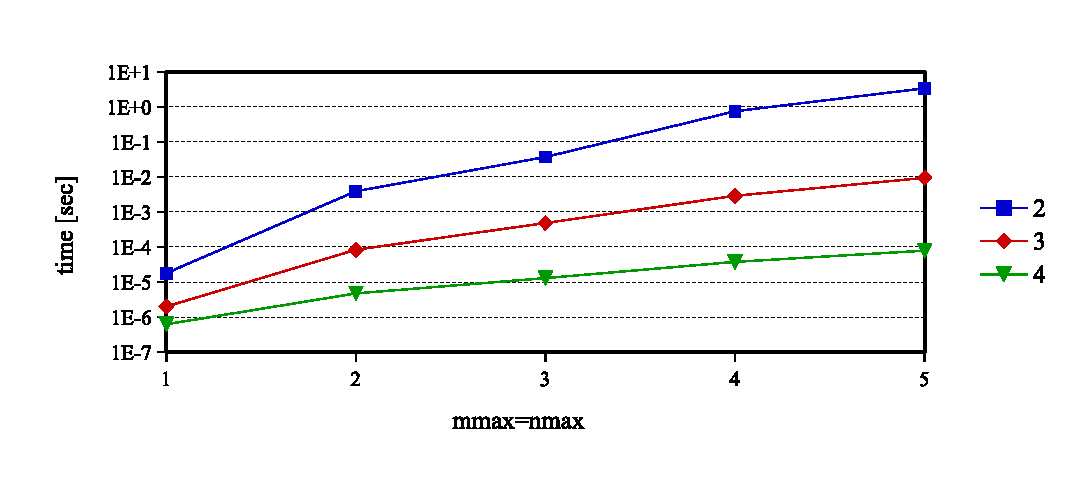
\includegraphics[bb=0bp 20bp 453bp 236bp,width=0.7\columnwidth]{_figure/results/k-kernel}
\par\end{centering}
\caption[Timing of a $k$-kernel]{Timing of a $k$-kernel (log scale)\label{fig:Timing-k-kernel}}
\end{figure}


\section{Entire iteration of $\mathcal{F}_{\mathrm{exc}}$ evaluation}

Apart from all the \texttt{\textbf{naive}} methods that will be discussed
in $\mathsection$\ref{subsec:Comparison-between-naive_standar},
figure \ref{fig:Entire-iteration} shows all the comparable \texttt{\textbf{convolution}}
timing data. We can see \texttt{\textbf{convolution\_standard}} is
the fastest algorithm, and \acs{OZ} equation is not the longest part
in the iteration. All the tests are performed for a $L=24$, $\mathrm{nfft}=72$
grid with 4 series: the three \texttt{\textbf{convolution}} methods
with $m_{\max}=n_{\max}$, and \texttt{\textbf{convolution\_standard}}
with $m_{\max}=5$, varying $n_{\max}$.

\begin{figure}[H]
\begin{centering}
\includegraphics[width=0.9\columnwidth]{_figure/results/branch_perf}
\par\end{centering}
\caption[Entire iteration of $\mathcal{F}_{\mathrm{exc}}$ evaluation]{Entire iteration of $\mathcal{F}_{\mathrm{exc}}$ evaluation: timing
overall / decomposition of timing for 1 iteration evaluation\label{fig:Entire-iteration}}
\end{figure}


\subsection{``naive'' methods and ``convolution\_pure\_angular''\label{subsec:Comparison-between-naive_standar}}

The \texttt{\textbf{naive\_standard}}, \texttt{\textbf{naive\_interpolation}},
and \texttt{\textbf{convolution\_pure\_angular}} methods share the
same processes out of the $k$-kernel. Table \ref{tab:Timing-loop-k}
shows the timing of loop $k$ of these three methods. It indicates
that \texttt{\textbf{convolution\_pure\_angular}} takes far less time
than the other two methods, of which the loop $k$ takes time in the
same order of magnitude as the rest of iteration. And once $m_{\max}\geq2$,
\texttt{\textbf{naive\_interpolation}} is faster than \texttt{\textbf{naive\_standard}}.
Note that order 2 of \texttt{\textbf{naive\_interpolation}} can give
good results for a \acs{DCF} of $n_{\max}=5$. So in every case of
\texttt{\textbf{naive}} methods, \texttt{\textbf{naive\_interpolation}}
should be used. This verifies the conclusion of $k$-kernel test in
that the path (4) in figure \ref{fig:k-kernel} is the fastest.

\begin{table}[H]
\begin{centering}
\begin{tabular}{ccccc}
\toprule 
$m_{\max}$ & \texttt{\textbf{naive\_standard}} & \texttt{\textbf{naive\_interpolation}} & \texttt{\textbf{convo\_pure\_angular}} & \tableheadline{Other}\tabularnewline
\midrule
1 & 2.34 & 4.42 & 0.26 & 0.15\tabularnewline
2 & 365.95 & 209.12 & 1.09 & 1.43\tabularnewline
3 & 3295.00 & 752.70 & 2.37 & 1.85\tabularnewline
4 & too long & too long & 5.93 & 6.73\tabularnewline
5 & too long & too long & 10.36 & 7.73\tabularnewline
\bottomrule
\end{tabular}
\par\end{centering}
\caption[Timing of loop $k$]{Timing {[}sec{]} of loop $k$ of ``naive\_standard'', ``naive\_interpolation''
and ``convolution\_pure\_angular'', and the rest of iteration\label{tab:Timing-loop-k}}
\end{table}


\subsection{``convolution\_standard'' and ``convolution\_pure\_angular''}

The comparison of \texttt{\textbf{convolution\_standard}} and \texttt{\textbf{convolution\_pure\_angular}}
appears in figure \ref{fig:comparison-pure_angular}. Their difference
lies in the inversion of \acs{FFT} and \acs{FGSHT}. We can see the
other parts are almost identical, but the implementation of \acs{FFT}
is different in terms of time. Because in \texttt{\textbf{convolution\_standard}}
the number of \acs{FE} we need for \acs{FFT} is the number of projections,
and in \texttt{\textbf{convolution\_pure\_angular}} it is the number
of angular grid nodes. As there are fewer projections than angular
nodes, \texttt{\textbf{convolution\_standard}} reasonably takes less
time. The stair form of the \texttt{\textbf{pure\_angular}} curve
is due to the grid $\Psi$, which takes $\left\lfloor m_{\max}/2\right\rfloor $
points in the presence of $\mathrm{C}_{2v}$ symmetry. Projections
are less sensible.

\begin{figure}[H]
\begin{centering}
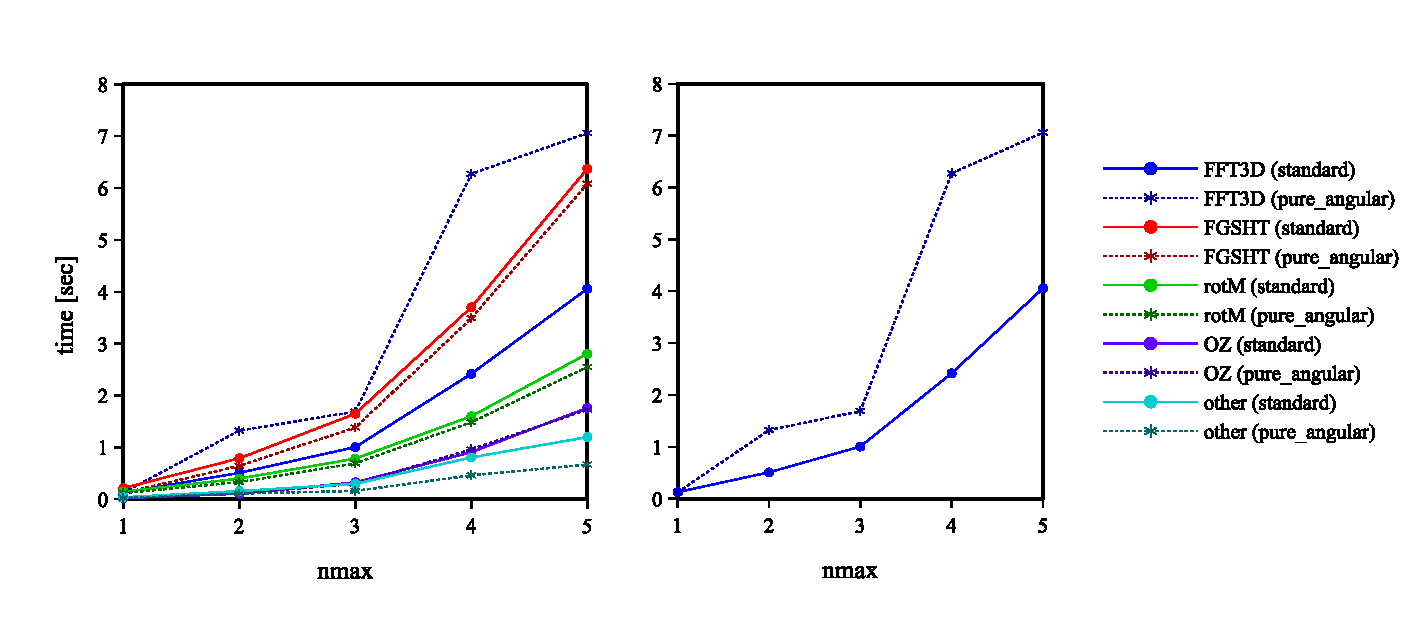
\includegraphics[bb=0bp 20bp 667bp 268bp,width=1\columnwidth]{_figure/results/pure_angular}
\par\end{centering}
\caption[Performance comparison of ``convolution\_standard'' and ``convolution\_pure\_angular'']{Performance comparison of \texttt{\textbf{convolution\_standard}}
and \texttt{\textbf{convolution\_pure\_angular\label{fig:comparison-pure_angular}}}}
\end{figure}


\subsection{``convolution\_standard'' and ``convolution\_asymm''}

We compare\texttt{\textbf{ convolution\_standard}} and \texttt{\textbf{convolution\_asymm}}
in figure \ref{fig:comparison-asymm}. The difference is that \texttt{\textbf{standard}}
calculates a half $k$ in the $k$-loop and \texttt{\textbf{asymm}}
calculates all $k$ in the $k$-loop. They share the same process
of \acs{FGSHT}; for the processes in a $k$-loop (rotM, OZ) \texttt{\textbf{asymm}}
always takes longer time. As in \texttt{\textbf{asymm}} we calculate
the \acs{FFT} for all the projections and in \texttt{\textbf{standard}}
we calculate only a half projections with $\mu\geq0$, the time consumed
by \acs{FFT} is also different.

\begin{figure}[H]
\begin{centering}
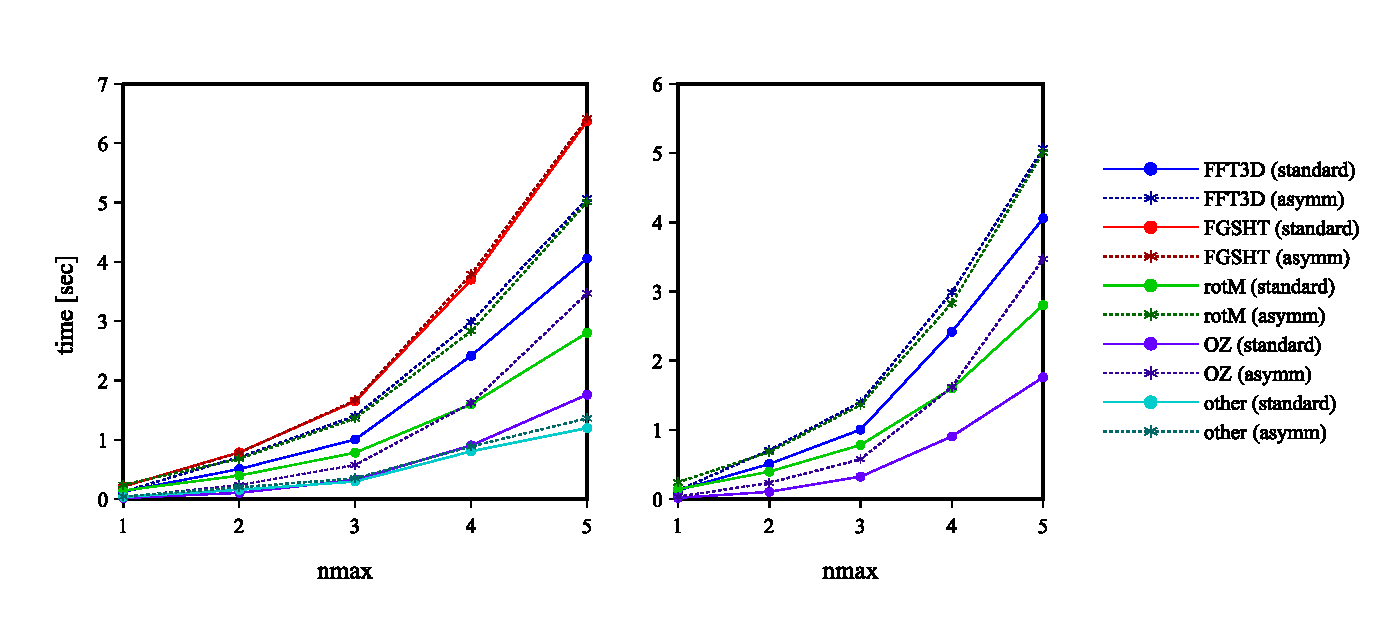
\includegraphics[bb=0bp 20bp 648bp 268bp,width=1\columnwidth]{_figure/results/asymm}
\par\end{centering}
\caption[Performance comparison of ``convolution\_standard'' and ``convolution\_asymm'']{Performance comparison of \texttt{\textbf{convolution\_standard}}
and \texttt{\textbf{convolution\_asymm\label{fig:comparison-asymm}}}}
\end{figure}


\subsection{Distinction of $m_{\max}$ and $n_{\max}$}

The comparison of $m_{\max}=n_{\max}$ and $m_{\max}=5$ for\texttt{\textbf{
convolution\_standard}} is shown in figure \ref{fig:comparison-nmax}.
We see that the choice of quadrature order $m_{\max}$ only affects
the \acs{FGSHT} process and the lecture/storage of density variable
(other). The time taken by extra order $m_{\max}$ is not cost-free,
as discussed in last section, it is fully recommended to use $m_{\max}=n_{\max}$.

\begin{figure}[H]
\begin{centering}
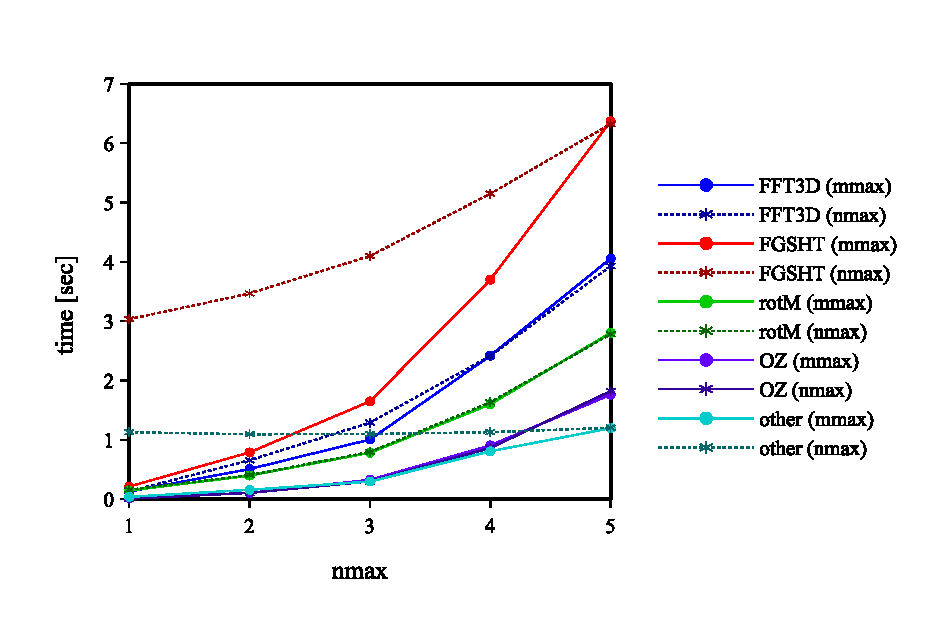
\includegraphics[bb=0bp 20bp 639bp 268bp,width=1\columnwidth]{_figure/results/nmax}
\par\end{centering}
\caption[Performance comparison of ``convolution\_standard'' for $m_{\max}=n_{\max}$
and $m_{\max}=5$]{Performance comparison of \texttt{\textbf{convolution\_standard}}
for $m_{\max}=n_{\max}$ and $m_{\max}=5$\label{fig:comparison-nmax}}
\end{figure}


\section{Global view of the code performance}

\begin{figure}[H]
\begin{centering}
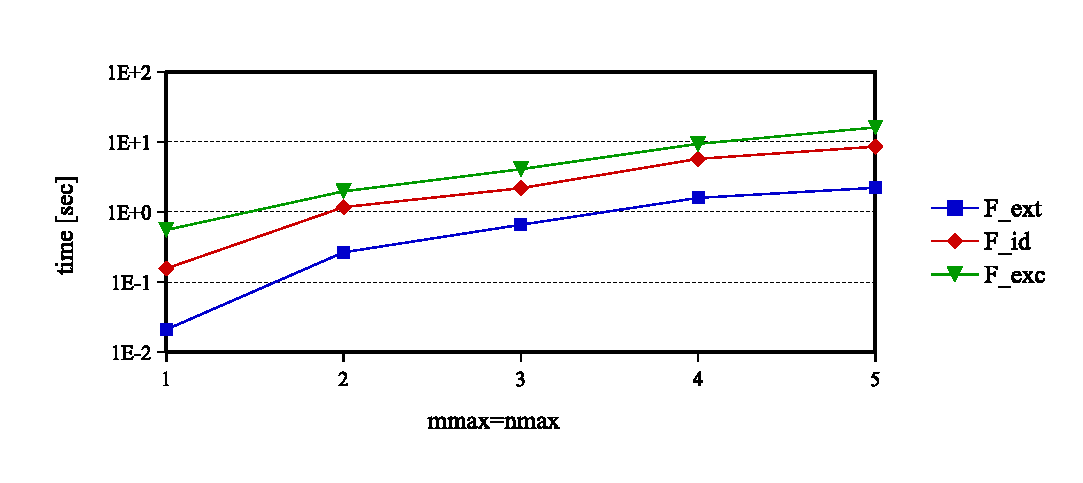
\includegraphics[bb=0bp 20bp 453bp 236bp,scale=0.7]{_figure/results/global_perf}
\par\end{centering}
\caption[Timing of the whole $\mathcal{F}$ iteration]{Timing of the whole $\mathcal{F}$ iteration with $\mathrm{nfft}/L=72/24$
grid (log scale)}
\end{figure}

Note that this is for an ion solute. $\mathcal{F}_{\mathrm{ext}}$
can be very slow if the solute have a very complex form.

We can see that \texttt{\textbf{convolution\_standard}} is the fastest.
The \texttt{\textbf{convolution}} methods are orders of magnitude
faster than \texttt{\textbf{naive}} methods. The evaluation of $\mathcal{F}_{\mathrm{exc}}$
is at the same order of magnitude than other two terms and the same
dependency on angular grid.


\ctparttext{Only a few applications are made due to the time limit of this thesis,
concluding\\
\medskip{}
Section {[}ref{]} to show the capability of MDFT to calculate ions
and small molecules.\\
\medskip{}
Section {[}ref{]} to show a qualitative influence of polar solvent
on the reaction including metal-oxo centre.}

\part{Applications}


\chapter{Comparison to MD simulation\label{chpt:ions}}

In the last chapter, we proved that \acs{MDFT} is capable of
correctly predicting solvation properties of LJ centers, single ions
and linear solutes compared to \acs{IET}. In this section, we will
compare them to \acs{MD} and experimental results. All the solutes
are optimized with the fast \texttt{\textbf{convolution\_standard}}
algorithm, with implicitly $L=24$ $\textrm{Å}$, $\mathrm{nfft}=72$,
$m_{\max}=n_{\max}$ unless otherwise specified. Comparison to the
dipole method is also involved, as we should justify that the increase
of computing cost when going from $n_{\max}=1$ to $n_{\max}>1$ is
counterbalanced by the ability to produce better results. 

\section{LJ centers}

The \acs{RDF}s of rare gases calculated in $\mathsection$\ref{tab:Free-energy-rare-gas}
are compared to \acs{MD} in figure \ref{fig:rare-gazz} using $n_{\max}=3$
to 5. The structures of different $n_{\max}$ is almost identical.
Comparing to \acs{MD}, it seems there is no improvement over the dipole method 
in ref \citep{Zhao_2011} or to calculation involving
$c_{00}^{000}$ only \citep{levesque_scalar_2012}. This kind of disagreement
in curve shape is regarded as a known default of \acs{HNC} (or \acs{HRF})
approximation.

\begin{figure}[h]
\begin{centering}
\includegraphics[width=0.95\columnwidth]{_figure/results/rare_gaz}
\par\end{centering}
\caption{\acs{RDF} of rare gasses compared to \acs{MD} result\label{fig:rare-gazz}}
\end{figure}


\section{Charged $\mathrm{CH_{4}}$ series}

The comparison between the \acs{RDF}s obtained from \acs{MDFT} with
\acs{MD} results for charged $\mathrm{CH_{4}}$ series are shown
in figure \ref{fig:Comparison-to-MD}. We can see that for positive
charges, the complete $n_{\max}=5$ gives much better results compared
to the dipole method, which itself almost agrees with \acs{MD} results.
For negative charges, $n_{\max}=5$ gives nearly the same result as
dipole method, while the \acs{MD} results are more smooth. Still the
first peak of the \acs{MDFT} results seems to be in a good position.
We can conclude that the complete \acs{DCF} gives a large improvement
for positive charged ions.

\begin{figure}[h]
\begin{centering}
\includegraphics[width=1\columnwidth]{_figure/results/ch4_md}
\par\end{centering}
\caption{\acs{RDF} of charged $\mathrm{CH_{4}}$ series compared to \acs{MD}
result\label{fig:Comparison-to-MD}}
\end{figure}


\section{Solvation free energy of single ions}

\marginpar{We consider that in a macroscopic system, the fluctuation of $N$
and $V$ are negligible, and all kinds of free energies become the
same. \citep{ensemble_thermo}}From the previous paragraph we can see the \acs{RDF} for positive ions are in good
agreement with \acs{MD} results. However, the free energy is more
difficult to compare, as there are several finite-size corrections
for single ions, depending on for example box length and charge; besides,
the free energy depends largely on the input LJ parameters of the
ions, which is independent to the method.

Table \ref{tab:single-ions} gives some independent experimental
and \acs{MD} simulation results of solvation free energy as well
as the positions of the first maximum of the \acs{RDF} for alkali
and halide ions. We can see that the experimental data themselves
vary a lot. Furthermore the LJ parameters for ions in the literature
are extremely dispersed. Therefore, we focused on a single series
of force field parameters for halide anions and alkali cations taken
from ref \citep{horinek_rational_2009} based on SPC/E water, as shown
in table \ref{tab:single-ions}. 

\begin{table}[h]
\begin{centering}
\begin{tabular*}{1\linewidth}{@{\extracolsep{\fill}}ccccccccc}
\toprule 
\addlinespace[-0.17em]
\tableheadline{{\footnotesize{}Ion}} & {\scriptsize{}$-\Delta G_{\mathrm{solv}}^{\mathrm{exp}}$\textsuperscript{{\scriptsize{}(a)}}} & {\scriptsize{}$-\Delta F_{\mathrm{solv}}^{\mathrm{exp}}$\textsuperscript{{\scriptsize{}(b)}}} & {\scriptsize{}$-\Delta G_{\mathrm{solv}}^{\mathrm{exp}}$\textsuperscript{{\scriptsize{}(c)}}} & {\scriptsize{}$R_{1}$\textsuperscript{{\scriptsize{}(d)}}} & {\scriptsize{}$\sigma$ $[\textrm{Å}]$\textsuperscript{{\scriptsize{}(e)}}} & {\scriptsize{}$\epsilon$ {[}$\mathrm{kJ\cdot mol^{-1}}${]}\textsuperscript{{\scriptsize{}(e)}}} & {\scriptsize{}$-\Delta G_{\mathrm{solv}}^{\mathrm{MD}}$\textsuperscript{{\scriptsize{}(e)}}} & {\scriptsize{}$R_{1}^{\mathrm{MD}}$\textsuperscript{{\scriptsize{}(e)}}}\tabularnewline
\midrule 
\addlinespace[-0.33em]
{\scriptsize{}$\mathrm{F^{-}}$} & {\scriptsize{}465} & {\scriptsize{}374.5} & {\scriptsize{}428.8} & {\scriptsize{}2.08} & {\scriptsize{}3.30} & {\scriptsize{}0.55} & {\scriptsize{}-430} & {\scriptsize{}2.74}\tabularnewline
\addlinespace[-0.33em]
{\scriptsize{}$\mathrm{Cl^{-}}$} & {\scriptsize{}340} & {\scriptsize{}318.4} & {\scriptsize{}304.2} & {\scriptsize{}2.36} & {\scriptsize{}3.78} & {\scriptsize{}0.52} & {\scriptsize{}-306} & {\scriptsize{}3.23}\tabularnewline
\addlinespace[-0.33em]
{\scriptsize{}$\mathrm{Br^{-}}$} & {\scriptsize{}315} & {\scriptsize{}289.5} & {\scriptsize{}227.4} & {\scriptsize{}2.80} & {\scriptsize{}4.00} & {\scriptsize{}0.37} & {\scriptsize{}-279} & {\scriptsize{}3.35}\tabularnewline
\addlinespace[-0.33em]
{\scriptsize{}$\mathrm{I^{-}}$ } & {\scriptsize{}275} & {\scriptsize{}252.3} & {\scriptsize{}240.0} & {\scriptsize{}2.89} & {\scriptsize{}4.25} & {\scriptsize{}0.32} & {\scriptsize{}-241} & {\scriptsize{}3.55}\tabularnewline
\addlinespace[-0.33em]
{\scriptsize{}$\mathrm{Li^{+}}$ } & {\scriptsize{}475} & {\scriptsize{}511.0} & {\scriptsize{}529.4} & {\scriptsize{}3.14} & {\scriptsize{}3.02} & {\scriptsize{}0.02} & {\scriptsize{}-520} & {\scriptsize{}1.91}\tabularnewline
\addlinespace[-0.33em]
{\scriptsize{}$\mathrm{Na^{+}}$ } & {\scriptsize{}365} & {\scriptsize{}411.5} & {\scriptsize{}423.8} & {\scriptsize{}2.63} & {\scriptsize{}3.49} & {\scriptsize{}0.02} & {\scriptsize{}-414} & {\scriptsize{}2.28}\tabularnewline
\addlinespace[-0.33em]
{\scriptsize{}$\mathrm{K^{+}}$ } & {\scriptsize{}295} & {\scriptsize{}337.2} & {\scriptsize{}352.0} & {\scriptsize{}3.19} & {\scriptsize{}3.85} & {\scriptsize{}0.02} & {\scriptsize{}-347} & {\scriptsize{}2.54}\tabularnewline
\addlinespace[-0.33em]
{\scriptsize{}$\mathrm{Rb^{+}}$ } & {\scriptsize{}275} & {\scriptsize{}316.0} & {\scriptsize{}329.3} & {\scriptsize{}3.37} & {\scriptsize{}no data} & {\scriptsize{}no data} & {\scriptsize{}no data} & {\scriptsize{}no data}\tabularnewline
\addlinespace[-0.33em]
{\scriptsize{}$\mathrm{Cs^{+}}$ } & {\scriptsize{}250} & {\scriptsize{}283.8} & {\scriptsize{}no data} & {\scriptsize{}3.65} & {\scriptsize{}4.17} & {\scriptsize{}0.02} & {\scriptsize{}-300} & {\scriptsize{}2.79}\tabularnewline
\bottomrule
\end{tabular*}
\par\end{centering}
\caption[Free energy and first maximum of ion-water oxygen \acs{RDF} for alkali
and halide ions from experimental and \acs{MD} simulation results]{Free energy $[\mathrm{kJ\cdot mol^{-1}}]$ and first maximum of ion-water
oxygen \acs{RDF} $[\textrm{Å}]$ for alkali and halide ions from
experimental and \acs{MD} simulation result. (a). Ref \citep{MARCUS1994111}.
(b). Ref \citep{Noyes_1962}. (c) Ref \citep{tissandier_protons_1998}.
(e) Ref \citep{horinek_rational_2009} from \acs{MD} simulation.
(d) Ref \citep{Marcus_1988}.\label{tab:single-ions}}

\vspace{0.5cm}

\begin{centering}
\begin{tabular*}{1\linewidth}{@{\extracolsep{\fill}}ccccccc}
\toprule 
\addlinespace[-0.17em]
\tableheadline{{\footnotesize{}Ion}} & {\scriptsize{}$\Delta G_{\mathrm{solv}}^{\mathrm{MD}}$} & {\scriptsize{}$\Delta\varOmega_{\mathrm{solv}}^{\mathrm{dipole}}$} & {\scriptsize{}$\Delta\varOmega_{\mathrm{solv}}^{\mathrm{nmax3}}$} & {\scriptsize{}$R_{1}^{\mathrm{MD}}$} & {\scriptsize{}$R_{1}^{\mathrm{dipole}}$} & {\scriptsize{}$R_{1}^{\mathrm{nmax3}}$}\tabularnewline
\midrule 
\addlinespace[-0.33em]
{\scriptsize{}$\mathrm{F^{-}}$ } & {\scriptsize{}-430} & {\scriptsize{}diverge} & {\scriptsize{}-368.5} & {\scriptsize{}2.74} & {\scriptsize{}-} & {\scriptsize{}2.71}\tabularnewline
\addlinespace[-0.33em]
{\scriptsize{}$\mathrm{Cl^{-}}$ } & {\scriptsize{}-306} & {\scriptsize{}diverge} & {\scriptsize{}-297.3} & {\scriptsize{}3.23} & {\scriptsize{}-} & {\scriptsize{}2.88}\tabularnewline
\addlinespace[-0.33em]
{\scriptsize{}$\mathrm{Br^{-}}$ } & {\scriptsize{}-279} & {\scriptsize{}diverge} & {\scriptsize{}-278.3} & {\scriptsize{}3.35} & {\scriptsize{}-} & {\scriptsize{}2.96}\tabularnewline
\addlinespace[-0.33em]
{\scriptsize{}$\mathrm{I^{-}}$ } & {\scriptsize{}-241} & {\scriptsize{}diverge} & {\scriptsize{}-253.4} & {\scriptsize{}3.55} & {\scriptsize{}-} & {\scriptsize{}3.12}\tabularnewline
\addlinespace[-0.33em]
{\scriptsize{}$\mathrm{Li^{+}}$ } & {\scriptsize{}-520} & {\scriptsize{}-707.7} & {\scriptsize{}-405.3} & {\scriptsize{}1.91} & {\scriptsize{}2.46} & {\scriptsize{}2.38}\tabularnewline
\addlinespace[-0.33em]
{\scriptsize{}$\mathrm{Na^{+}}$ } & {\scriptsize{}-414} & {\scriptsize{}-621.8} & {\scriptsize{}-366.0} & {\scriptsize{}2.28} & {\scriptsize{}2.54} & {\scriptsize{}2.54}\tabularnewline
\addlinespace[-0.33em]
{\scriptsize{}$\mathrm{K^{+}}$ } & {\scriptsize{}-347} & {\scriptsize{}-559.1} & {\scriptsize{}-338.4} & {\scriptsize{}2.54} & {\scriptsize{}2.63} & {\scriptsize{}2.70}\tabularnewline
\addlinespace[-0.33em]
{\scriptsize{}$\mathrm{Cs^{+}}$ } & {\scriptsize{}-300} & {\scriptsize{}-508.8} & {\scriptsize{}-316.1} & {\scriptsize{}2.79} & {\scriptsize{}2.88} & {\scriptsize{}2.88}\tabularnewline
\bottomrule
\end{tabular*}
\par\end{centering}
\caption[Free energies and first \acs{RDF} maximum of single ions from \acs{MDFT}
results]{Free energies $[\mathrm{kJ\cdot mol^{-1}}]$ and first \acs{RDF}
maximum $[\textrm{Å}]$ of single ions from \acs{MDFT} results compared
to \acs{MD} results \label{tab:free-energy-single-ions}}
\end{table}

The results shows that the free energies given by \acs{MDFT} are not
perfect, but lie in the same order of magnitude as \acs{MD} for $\mathrm{Cl}^{-}$
to $\mathrm{I}^{-}$ and $\mathrm{K}^{+}$ to $\mathrm{Cs}^{+}$.
They are much less convincing for small ions such as $\mathrm{F}^{-}$,
$\mathrm{Li}^{+}$ and $\mathrm{Na}^{+}$. Besides, the results with
a \acs{DCF} at $n_{\max}=3$ work better than the dipolar approximation,
which is a positive sign for our developments. In contrast, there
is no improvement in terms of position of the first solvation maximum.
Note that for this quantity, the agreement between experimental data
and \acs{MD} is not obvious either. 

\section{Small molecules}

\acs{MDFT} calculations involving some small molecular solutes were
also generated to compare to \acs{MD}; the chosen solutes are shown
in figure \ref{fig:Test-solutes-2} and defined in table \ref{tab:Parameters-of-test-solutes-2}.
Note that a certain proportion of them have a non-linear, 3-dimensional
geometry which could not be handled by the molecular \acs{IET}; this
shows the advantage of the general 3D-\acs{MDFT} approach adopted
in this thesis and the new algorithm that we have developed in this
context.

Figure \ref{fig:Site-O} gives the site-site \acs{RDF}s (solute site
to water O site) for $n_{\max}=4$, the dipolar approximation ($n_{\max}=1$),
and \acs{MD} for these test solutes. It is shown that in most
of the cases, $n_{\max}=4$ does give equivalent or better results
than the dipolar order, apart from the cases of water, and especially
SPC/E water. In methanol, the dipole method diverges. For most solutes,
the comparison to \acs{MD} is far from perfect but can be qualified
as satisfactory in reproducing the - sometimes complex - shape of
the \acs{RDF}s and the main peaks positions. This statement is especially
true for benzene and pyrimidine, for example. For hydrophobic molecules
or molecules with hydrophobic sites (alkanes, oxygen, nitrogen)
one recovers the slight underestimation of the first peak position
and the overestimation of peak height already remarked for
rare gases; this is a clear defect of \acs{HNC}. The case of molecules
giving rise to hydrogen bonds to water (e.g. methanol, or water in
water) is more problematic and subtle. Here the dipolar approximation
gives a first peak for the water oxygen around the O-site that is
too high but has the correct width, whereas $n_{\max}=4$ shifts the
first peak to higher values and makes it too wide (a sort of merge
of the first and second peak, an effect even clearer for methanol).
The H-O first peak, on the other hand, is at a correct position but
underestimated, both for water and methanol. The tetrahedral order
around a water solute is not correctly reproduced, although the correct
balance to get the right structure is subtle and does not appear too
far. 

For the purpose of showing the ability of \acs{MDFT} to calculate
3D solute structure, we display 3D solvent densities for specific
solutes in figure \ref{fig:Volume-slice-of} and \ref{fig:Iso-surface-of-solvent}.
Figure \ref{fig:Iso-surface-of-solvent} complements the discussion
given just above concerning the expected tetrahedral structure around
a water molecule in water. That structure can indeed be detected for
SPC/E water and even more so for the TIP4P model. In SPC/E water,
there is more density than expected on the north pole, and this piece
of density disappears with the extra charge added on the TIP4P water.\\

\begin{figure}[H]
\begin{centering}
\includegraphics[width=1\columnwidth]{_figure/app_solute_var}
\par\end{centering}
\caption{Test solutes\label{fig:Test-solutes-2}}
\end{figure}

\begin{table}[H]
\begin{centering}
\begin{tabular*}{1\linewidth}{@{\extracolsep{\fill}}llrrrrrr}
\toprule 
\addlinespace[-0.17em]
\tableheadline{{\footnotesize{}Solute}} & \tableheadline{{\footnotesize{}Site}} & {\scriptsize{}$q$} & {\scriptsize{}$\sigma$ $[\textrm{Å}]$} & {\scriptsize{}$\epsilon$ {[}$\mathrm{kJ\cdot mol^{-1}}${]}} & {\scriptsize{}$x$ $[\textrm{Å}]$} & {\scriptsize{}$y$ $[\textrm{Å}]$} & {\scriptsize{}$z$ $[\textrm{Å}]$}\tabularnewline
\midrule 
\addlinespace[-0.33em]
{\scriptsize{}Acetone \citep{jorgensen_relative_1990}} & {\scriptsize{}CH\textsubscript{3}} & {\scriptsize{}0.062} & {\scriptsize{}3.91} & {\scriptsize{}0.6694} & {\scriptsize{}1.2810} & {\scriptsize{}0.7024} & {\scriptsize{}-0.0002}\tabularnewline
\addlinespace[-0.17em]
\addlinespace[-0.33em]
 & {\scriptsize{}C} & {\scriptsize{}0.300} & {\scriptsize{}3.75} & {\scriptsize{}0.4393} & {\scriptsize{}0.0101} & {\scriptsize{}-0.0872 } & {\scriptsize{}0.0106 }\tabularnewline
\addlinespace[-0.17em]
\addlinespace[-0.33em]
 & {\scriptsize{}O} & {\scriptsize{}-0.424} & {\scriptsize{}2.96} & {\scriptsize{}0.8796} & {\scriptsize{}0.0103} & {\scriptsize{}-1.3171 } & {\scriptsize{}-0.0102 }\tabularnewline
\addlinespace[-0.17em]
\addlinespace[-0.33em]
 & {\scriptsize{}CH\textsubscript{3}} & {\scriptsize{}0.062} & {\scriptsize{}3.91} & {\scriptsize{}0.6694} & {\scriptsize{}-1.2813} & {\scriptsize{}0.7019} & {\scriptsize{}-0.0002}\tabularnewline
\addlinespace[-0.17em]
\midrule 
\addlinespace[-0.33em]
{\scriptsize{}Acetonitrile }\textcolor{red}{\scriptsize{}{[}ref{]}} & {\scriptsize{}CH\textsubscript{3}} & {\scriptsize{}0.269 } & {\scriptsize{}3.6 } & {\scriptsize{}1.590 } & {\scriptsize{}0.0000} & {\scriptsize{}0.0000} & {\scriptsize{}-1.3254 }\tabularnewline
\addlinespace[-0.17em]
\addlinespace[-0.33em]
 & {\scriptsize{}C} & {\scriptsize{}0.129} & {\scriptsize{}3.4 } & {\scriptsize{}0.416 } & {\scriptsize{}0.0000} & {\scriptsize{}0.0000} & {\scriptsize{}0.1346}\tabularnewline
\addlinespace[-0.17em]
\addlinespace[-0.33em]
 & {\scriptsize{}N} & {\scriptsize{}-0.398 } & {\scriptsize{}3.3 } & {\scriptsize{}0.416 } & {\scriptsize{}0.0000} & {\scriptsize{}0.0000} & {\scriptsize{}1.3046}\tabularnewline
\addlinespace[-0.17em]
\midrule 
\addlinespace[-0.33em]
{\scriptsize{}Ammonia \citep{Diraison_1999}} & {\scriptsize{}N} & {\scriptsize{}0.000 } & {\scriptsize{}3.4 } & {\scriptsize{}1.164 } & {\scriptsize{}0.000000} & {\scriptsize{}0.000000} & {\scriptsize{}0.000000}\tabularnewline
\addlinespace[-0.17em]
\addlinespace[-0.33em]
 & {\scriptsize{}X} & {\scriptsize{}-1.386} & {\scriptsize{}0.0} & {\scriptsize{}0.000} & {\scriptsize{}0.000000} & {\scriptsize{}0.000000} & {\scriptsize{}-0.156000}\tabularnewline
\addlinespace[-0.17em]
\addlinespace[-0.33em]
 & {\scriptsize{}H} & {\scriptsize{}0.462} & {\scriptsize{}0.0} & {\scriptsize{}0.000} & {\scriptsize{}-0.937790} & {\scriptsize{}0.000000} & {\scriptsize{}-0.381449}\tabularnewline
\addlinespace[-0.17em]
\addlinespace[-0.33em]
 & {\scriptsize{}H} & {\scriptsize{}0.462} & {\scriptsize{}0.0} & {\scriptsize{}0.000} & {\scriptsize{}0.468895} & {\scriptsize{}0.812150} & {\scriptsize{}-0.381449}\tabularnewline
\addlinespace[-0.17em]
\addlinespace[-0.33em]
 & {\scriptsize{}H} & {\scriptsize{}0.462} & {\scriptsize{}0.0} & {\scriptsize{}0.000} & {\scriptsize{}0.468895} & {\scriptsize{}-0.812150} & {\scriptsize{}-0.381449}\tabularnewline
\addlinespace[-0.17em]
\midrule 
\addlinespace[-0.33em]
{\scriptsize{}Benzene \citep{Chipot_1996}} & {\scriptsize{}C} & {\scriptsize{}-0.138} & {\scriptsize{}1.908 } & {\scriptsize{}0.35980 } & {\scriptsize{}1.386 } & {\scriptsize{}0.000} & {\scriptsize{}0.000}\tabularnewline
\addlinespace[-0.17em]
\addlinespace[-0.33em]
{\scriptsize{}(charged)} & {\scriptsize{}C} & {\scriptsize{}-0.138} & {\scriptsize{}1.908 } & {\scriptsize{}0.35980 } & {\scriptsize{}0.693} & {\scriptsize{}-1.200} & {\scriptsize{}0.000}\tabularnewline
\addlinespace[-0.17em]
\addlinespace[-0.33em]
 & {\scriptsize{}C} & {\scriptsize{}-0.138} & {\scriptsize{}1.908 } & {\scriptsize{}0.35980 } & {\scriptsize{}-0.693} & {\scriptsize{}-1.200} & {\scriptsize{}0.000}\tabularnewline
\addlinespace[-0.17em]
\addlinespace[-0.33em]
 & {\scriptsize{}C} & {\scriptsize{}-0.138} & {\scriptsize{}1.908 } & {\scriptsize{}0.35980 } & {\scriptsize{}-1.386} & {\scriptsize{}0.000} & {\scriptsize{}0.000}\tabularnewline
\addlinespace[-0.17em]
\addlinespace[-0.33em]
 & {\scriptsize{}C} & {\scriptsize{}-0.138} & {\scriptsize{}1.908 } & {\scriptsize{}0.35980 } & {\scriptsize{}-0.693} & {\scriptsize{}1.200} & {\scriptsize{}0.000}\tabularnewline
\addlinespace[-0.17em]
\addlinespace[-0.33em]
 & {\scriptsize{}C} & {\scriptsize{}-0.138} & {\scriptsize{}1.908 } & {\scriptsize{}0.35980 } & {\scriptsize{}0.693} & {\scriptsize{}1.200} & {\scriptsize{}0.000}\tabularnewline
\addlinespace[-0.17em]
\addlinespace[-0.33em]
 & {\scriptsize{}H} & {\scriptsize{}0.138 } & {\scriptsize{}1.459} & {\scriptsize{}0.06276 } & {\scriptsize{}2.462} & {\scriptsize{}0.000} & {\scriptsize{}0.000}\tabularnewline
\addlinespace[-0.17em]
\addlinespace[-0.33em]
 & {\scriptsize{}H} & {\scriptsize{}0.138 } & {\scriptsize{}1.459} & {\scriptsize{}0.06276 } & {\scriptsize{}1.231} & {\scriptsize{}-2.132} & {\scriptsize{}0.000}\tabularnewline
\addlinespace[-0.17em]
\addlinespace[-0.33em]
 & {\scriptsize{}H} & {\scriptsize{}0.138 } & {\scriptsize{}1.459} & {\scriptsize{}0.06276 } & {\scriptsize{}-1.231} & {\scriptsize{}-2.132} & {\scriptsize{}0.000}\tabularnewline
\addlinespace[-0.17em]
\addlinespace[-0.33em]
 & {\scriptsize{}H} & {\scriptsize{}0.138 } & {\scriptsize{}1.459} & {\scriptsize{}0.06276 } & {\scriptsize{}-2.462} & {\scriptsize{}0.000} & {\scriptsize{}0.000}\tabularnewline
\addlinespace[-0.17em]
\addlinespace[-0.33em]
 & {\scriptsize{}H} & {\scriptsize{}0.138 } & {\scriptsize{}1.459} & {\scriptsize{}0.06276 } & {\scriptsize{}-1.231} & {\scriptsize{}2.132} & {\scriptsize{}0.000}\tabularnewline
\addlinespace[-0.17em]
\addlinespace[-0.33em]
 & {\scriptsize{}H} & {\scriptsize{}0.138 } & {\scriptsize{}1.459} & {\scriptsize{}0.06276 } & {\scriptsize{}1.231} & {\scriptsize{}2.132} & {\scriptsize{}0.000}\tabularnewline
\addlinespace[-0.17em]
\midrule 
\addlinespace[-0.33em]
{\scriptsize{}$\mathrm{CO_{2}}$ \citep{Harris_1995}} & {\scriptsize{}C} & {\scriptsize{}0.6512 } & {\scriptsize{}2.76} & {\scriptsize{}0.234} & {\scriptsize{}0.000 } & {\scriptsize{}0.000 } & {\scriptsize{}0.000 }\tabularnewline
\addlinespace[-0.17em]
\addlinespace[-0.33em]
 & {\scriptsize{}O} & {\scriptsize{}-0.3256} & {\scriptsize{}3.03 } & {\scriptsize{}0.67} & {\scriptsize{}-1.149 } & {\scriptsize{}0.000 } & {\scriptsize{}0.000 }\tabularnewline
\addlinespace[-0.17em]
\addlinespace[-0.33em]
 & {\scriptsize{}O} & {\scriptsize{}-0.3256} & {\scriptsize{}3.03 } & {\scriptsize{}0.67} & {\scriptsize{}1.149 } & {\scriptsize{}0.000 } & {\scriptsize{}0.000 }\tabularnewline
\addlinespace[-0.17em]
\midrule 
\addlinespace[-0.33em]
{\scriptsize{}$\mathrm{O_{2}}$ \citep{Boutard200525}} & {\scriptsize{}O} & {\scriptsize{}0.0} & {\scriptsize{}3.1062} & {\scriptsize{}0.36 } & {\scriptsize{}-0.485} & {\scriptsize{}0.000 } & {\scriptsize{}0.000 }\tabularnewline
\addlinespace[-0.17em]
\addlinespace[-0.33em]
 & {\scriptsize{}O} & {\scriptsize{}0.0} & {\scriptsize{}3.1062} & {\scriptsize{}0.36 } & {\scriptsize{}0.485} & {\scriptsize{}0.000 } & {\scriptsize{}0.000 }\tabularnewline
\addlinespace[-0.17em]
\addlinespace[-0.33em]
 & {\scriptsize{}X} & {\scriptsize{}-2.1} & {\scriptsize{}0.00} & {\scriptsize{}0.00} & {\scriptsize{}-0.200} & {\scriptsize{}0.000 } & {\scriptsize{}0.000 }\tabularnewline
\addlinespace[-0.17em]
\addlinespace[-0.33em]
 & {\scriptsize{}X} & {\scriptsize{}-2.1} & {\scriptsize{}0.00} & {\scriptsize{}0.00} & {\scriptsize{}0.200} & {\scriptsize{}0.000 } & {\scriptsize{}0.000 }\tabularnewline
\addlinespace[-0.17em]
\addlinespace[-0.33em]
 & {\scriptsize{}X} & {\scriptsize{}4.2} & {\scriptsize{}0.00} & {\scriptsize{}0.00} & {\scriptsize{}0.000} & {\scriptsize{}0.000 } & {\scriptsize{}0.000 }\tabularnewline
\addlinespace[-0.17em]
\midrule 
\addlinespace[-0.33em]
{\scriptsize{}Ethane \citep{jorgensen_relative_1990}} & {\scriptsize{}CH\textsubscript{3}} & {\scriptsize{}0.0} & {\scriptsize{}3.775} & {\scriptsize{}0.8661} & {\scriptsize{}-0.756} & {\scriptsize{}0.000} & {\scriptsize{}0.000}\tabularnewline
\addlinespace[-0.17em]
\addlinespace[-0.33em]
 & {\scriptsize{}CH\textsubscript{3}} & {\scriptsize{}0.0} & {\scriptsize{}3.775} & {\scriptsize{}0.8661} & {\scriptsize{}0.756} & {\scriptsize{}0.000} & {\scriptsize{}0.000}\tabularnewline
\addlinespace[-0.17em]
\midrule 
\addlinespace[-0.33em]
{\scriptsize{}Methanol \citep{Schnabel_2007}} & {\scriptsize{}CH\textsubscript{3}} & {\scriptsize{}0.24746} & {\scriptsize{}3.7543} & {\scriptsize{}1.0027} & {\scriptsize{}-1.42460} & {\scriptsize{}0.000000} & {\scriptsize{}0.000000}\tabularnewline
\addlinespace[-0.17em]
\addlinespace[-0.33em]
 & {\scriptsize{}OH} & {\scriptsize{}-0.67874} & {\scriptsize{}3.0300} & {\scriptsize{}0.7307} & {\scriptsize{}0.00000} & {\scriptsize{}0.000000} & {\scriptsize{}0.000000}\tabularnewline
\addlinespace[-0.17em]
\addlinespace[-0.33em]
 & {\scriptsize{}X} & {\scriptsize{}0.43128} & {\scriptsize{}0.0000} & {\scriptsize{}0.0000} & {\scriptsize{}0.30035} & {\scriptsize{}0.896104} & {\scriptsize{}0.000000}\tabularnewline
\addlinespace[-0.17em]
\midrule 
\addlinespace[-0.33em]
{\scriptsize{}$\mathrm{N_{2}}$ }\textcolor{red}{\scriptsize{}{[}ref{]}} & {\scriptsize{}N} & {\scriptsize{}-0.5075} & {\scriptsize{}3.30} & {\scriptsize{}0.30} & {\scriptsize{}-0.549} & {\scriptsize{}0.000} & {\scriptsize{}0.000}\tabularnewline
\addlinespace[-0.17em]
\addlinespace[-0.33em]
 & {\scriptsize{}N} & {\scriptsize{}-0.5075} & {\scriptsize{}3.30} & {\scriptsize{}0.30} & {\scriptsize{}0.549} & {\scriptsize{}0.000} & {\scriptsize{}0.000}\tabularnewline
\addlinespace[-0.17em]
\addlinespace[-0.33em]
 & {\scriptsize{}X} & {\scriptsize{}1.0150} & {\scriptsize{}0.00} & {\scriptsize{}0.00} & {\scriptsize{}0.000} & {\scriptsize{}0.000} & {\scriptsize{}0.000}\tabularnewline
\addlinespace[-0.17em]
\midrule 
\addlinespace[-0.33em]
{\scriptsize{}Propane }\textcolor{red}{\scriptsize{}{[}ref{]}} & {\scriptsize{}CH\textsubscript{3}} & {\scriptsize{}0.0} & {\scriptsize{}3.905} & {\scriptsize{}0.732} & {\scriptsize{}-1.25} & {\scriptsize{}-0.4417} & {\scriptsize{}0.0}\tabularnewline
\addlinespace[-0.17em]
\addlinespace[-0.33em]
 & {\scriptsize{}CH\textsubscript{2}} & {\scriptsize{}0.0} & {\scriptsize{}3.905} & {\scriptsize{}0.494} & {\scriptsize{}0.0} & {\scriptsize{}0.4417} & {\scriptsize{}0.0}\tabularnewline
\addlinespace[-0.17em]
\addlinespace[-0.33em]
 & {\scriptsize{}CH\textsubscript{3}} & {\scriptsize{}0.0} & {\scriptsize{}3.905} & {\scriptsize{}0.732} & {\scriptsize{}1.25} & {\scriptsize{}-0.4417} & {\scriptsize{}0.0}\tabularnewline
\addlinespace[-0.17em]
\midrule 
\addlinespace[-0.33em]
{\scriptsize{}Pyrimidine \citep{jorgensen_relative_1990}} & {\scriptsize{}N} & {\scriptsize{}-0.490} & {\scriptsize{}3.25} & {\scriptsize{}0.7113} & {\scriptsize{}1.2035} & {\scriptsize{}-0.6989} & {\scriptsize{}0.0000}\tabularnewline
\addlinespace[-0.17em]
\addlinespace[-0.33em]
 & {\scriptsize{}N} & {\scriptsize{}-0.490} & {\scriptsize{}3.25} & {\scriptsize{}0.7113} & {\scriptsize{}-1.2063} & {\scriptsize{}-0.6943} & {\scriptsize{}0.0000}\tabularnewline
\addlinespace[-0.17em]
\addlinespace[-0.33em]
 & {\scriptsize{}C\textsuperscript{2}H} & {\scriptsize{}0.410} & {\scriptsize{}3.75} & {\scriptsize{}0.4602} & {\scriptsize{}-0.0026} & {\scriptsize{}-1.2980} & {\scriptsize{}0.0001}\tabularnewline
\addlinespace[-0.17em]
\addlinespace[-0.33em]
 & {\scriptsize{}C\textsuperscript{3}H} & {\scriptsize{}0.245} & {\scriptsize{}3.75} & {\scriptsize{}0.4602} & {\scriptsize{}1.1692} & {\scriptsize{}0.6499} & {\scriptsize{}-0.0001}\tabularnewline
\addlinespace[-0.17em]
\addlinespace[-0.33em]
 & {\scriptsize{}C\textsuperscript{4}H} & {\scriptsize{}0.245} & {\scriptsize{}3.75} & {\scriptsize{}0.4602} & {\scriptsize{}-1.1666} & {\scriptsize{}0.6543} & {\scriptsize{}-0.0001}\tabularnewline
\addlinespace[-0.17em]
\addlinespace[-0.33em]
 & {\scriptsize{}C\textsuperscript{5}H} & {\scriptsize{}0.080} & {\scriptsize{}3.75} & {\scriptsize{}0.4602} & {\scriptsize{}0.0028} & {\scriptsize{}1.3870} & {\scriptsize{}0.0001}\tabularnewline
\addlinespace[-0.17em]
\midrule 
\addlinespace[-0.33em]
{\scriptsize{}SPC/E \citep{SPC/E}} & {\scriptsize{}O} & {\scriptsize{}-0.8476} & {\scriptsize{}3.165} & {\scriptsize{}0.65} & {\scriptsize{}0.000000} & {\scriptsize{}0.000000} & {\scriptsize{}0.0000000}\tabularnewline
\addlinespace[-0.17em]
\addlinespace[-0.33em]
 & {\scriptsize{}H} & {\scriptsize{}0.4238} & {\scriptsize{}0.000} & {\scriptsize{}0.00} & {\scriptsize{}0.816495} & {\scriptsize{}0.000000} & {\scriptsize{}0.5773525}\tabularnewline
\addlinespace[-0.17em]
\addlinespace[-0.33em]
 & {\scriptsize{}H} & {\scriptsize{}0.4238} & {\scriptsize{}0.000} & {\scriptsize{}0.00} & {\scriptsize{}-0.816495} & {\scriptsize{}0.000000} & {\scriptsize{}0.5773525}\tabularnewline
\addlinespace[-0.17em]
\midrule 
\addlinespace[-0.33em]
{\scriptsize{}TIP4P \citep{Abascal_2005}} & {\scriptsize{}O} & {\scriptsize{}0.0000} & {\scriptsize{}3.1589} & {\scriptsize{}0.775} & {\scriptsize{}0.00000} & {\scriptsize{}0.00000} & {\scriptsize{}0.00000}\tabularnewline
\addlinespace[-0.17em]
\addlinespace[-0.33em]
 & {\scriptsize{}H} & {\scriptsize{}0.5564} & {\scriptsize{}0.0000} & {\scriptsize{}0.000} & {\scriptsize{}0.75695} & {\scriptsize{}0.58588} & {\scriptsize{}0.00000}\tabularnewline
\addlinespace[-0.17em]
\addlinespace[-0.33em]
 & {\scriptsize{}H} & {\scriptsize{}0.5564} & {\scriptsize{}0.0000} & {\scriptsize{}0.000} & {\scriptsize{}-0.75695} & {\scriptsize{}0.58588} & {\scriptsize{}0.00000}\tabularnewline
\addlinespace[-0.17em]
\addlinespace[-0.33em]
 & {\scriptsize{}X} & {\scriptsize{}-1.1128} & {\scriptsize{}0.0000} & {\scriptsize{}0.000} & {\scriptsize{}0.00000} & {\scriptsize{}0.15460} & {\scriptsize{}0.00000}\tabularnewline
\bottomrule
\addlinespace[-0.17em]
\end{tabular*}
\par\end{centering}
\caption{Parameters of test solutes\label{tab:Parameters-of-test-solutes-2}}
\end{table}

\begin{figure}[H]
\begin{centering}
\includegraphics[width=1\columnwidth]{_figure/results/solute\lyxdot acetone-3}
\par\end{centering}
\begin{centering}
\includegraphics[width=1\columnwidth]{_figure/results/solute\lyxdot acetonitrile-3}
\par\end{centering}
\begin{centering}
\includegraphics[width=1\columnwidth]{_figure/results/solute\lyxdot ammonia-3}
\par\end{centering}
\begin{centering}
\includegraphics[width=1\columnwidth]{_figure/results/solute\lyxdot benzene-3}
\par\end{centering}
\caption[Site-O \acs{RDF} of test solutes]{Site-O \acs{RDF} of test solutes, with $m_{\max}=n_{\max}=4$, $L=24$
$\textrm{Å}$, $\mathrm{nfft}=72$. $\frac{1}{3}n_{\mathrm{bin}}$
is used in order to avoid noise.\label{fig:Site-O}}
\end{figure}

\begin{figure}[H]
\ContinuedFloat
\begin{centering}
\includegraphics[width=1\columnwidth]{_figure/results/solute\lyxdot carbondioxide-3}
\par\end{centering}
\begin{centering}
\includegraphics[width=1\columnwidth]{_figure/results/solute\lyxdot oxygen-3}
\par\end{centering}
\begin{centering}
\includegraphics[width=1\columnwidth]{_figure/results/solute\lyxdot ethane-3}
\par\end{centering}
\begin{centering}
\includegraphics[width=1\columnwidth]{_figure/results/solute\lyxdot methanol-3}
\par\end{centering}
\caption[]{Site-O \acs{RDF} of test solutes (continued)}
\end{figure}

\begin{figure}[H]
\ContinuedFloat
\begin{centering}
\includegraphics[width=1\columnwidth]{_figure/results/solute\lyxdot nitrogen-3}
\par\end{centering}
\begin{centering}
\includegraphics[width=1\columnwidth]{_figure/results/solute\lyxdot propane-3}
\par\end{centering}
\begin{centering}
\includegraphics[width=1\columnwidth]{_figure/results/solute\lyxdot pyrimidine-3}
\par\end{centering}
\begin{centering}
\includegraphics[width=1\columnwidth]{_figure/results/solute\lyxdot spce-3}
\par\end{centering}
\caption[]{Site-O \acs{RDF} of test solutes (continued)}
\end{figure}

\begin{figure}[H]
\ContinuedFloat
\begin{centering}
\includegraphics[width=1\columnwidth]{_figure/results/solute\lyxdot tip4p-3}
\par\end{centering}
\caption[]{Site-O \acs{RDF} of test solutes (continued)}
\end{figure}

\begin{figure}[H]
\begin{centering}
\includegraphics[width=0.7\columnwidth]{/Users/Hostiphre/Desktop/_M1116/_figure/results/solute\lyxdot pyrimidine\lyxdot snap}
\par\end{centering}
\caption{Volume slice of solvent number density $n(\mathbf{r})$ for pyrimidine\label{fig:Volume-slice-of}}
\end{figure}

\begin{figure}[H]
\subfloat[SPC/E water]{\begin{centering}
\includegraphics[width=0.45\columnwidth]{/Users/Hostiphre/Desktop/_M1116/_figure/results/solute\lyxdot spce\lyxdot snap}
\par\end{centering}
}\subfloat[TIP4P water]{\begin{centering}
\includegraphics[width=0.45\columnwidth]{/Users/Hostiphre/Desktop/_M1116/_figure/results/solute\lyxdot tip4p\lyxdot snap}
\par\end{centering}
}

\caption{Iso-surface of solvent number density $n(\mathbf{r})=2.4$ for test
water molecules\label{fig:Iso-surface-of-solvent}}
\end{figure}

\newpage{}

$ $



\chapter{Hydrogen Transfer Reaction of Mn-oxo: Role of Solvent in Reaction
Simulation\label{chpt:mnoxo}}

\section{Reinvestigation of the Manganese-oxo }

This is the case we talked about in the introduction, which is the
thesis of university , the motivation of this thesis


\ctparttext{The only one publication during this thesis}

\part{Conclusion and Perspectives}


\chapter{Conclusion\label{chpt:conclusion}}

Here is the publication during this thesis:

\bigskip{}

\noindent \begin{refsection}[ownpubs]
	\small
	\nocite{*}
	\printbibliography[heading=none]
\end{refsection}



\chapter{Perspectives\label{chpt:perspectives}}

The work is never perfect, a great deal of unfinished work and theories
linked to this thesis is presented here. 

\section{Reduce memory footprint in MDFT}

The total CPU time to implement a \acs{MDFT} minimization using the
\texttt{\textbf{convolution}} algorithms is typically 1 to 30 minutes
according to the resolution of grid. But the memory consumed for such
a process is typically 1 to 20 G of RAM. This is mainly due to the
minimizer L-BFGS-B, which firstly needs to store several steps of
information during the iterations, and secondly is in double precision.
It is to say that the density variable $\rho(\mathbf{r},\mathbf{\Omega})$
and the gradient also need to be stored in double precision, and if
not, as I tested, it leads to divergence. In addition, during the
evaluation of the functional, the memory for at most 3 times $\rho(\mathbf{r},\mathbf{\Omega})$
needs to be open simultaneously.

There are two ways to get over this memory limit, and both of them
need to modify the L-BFGS-B minimizer, which is a ``blackbox'',
in Fortran 77. The simplest way is to change the double precision
to single in the L-BFGS-B minimizer; this action can reduce the memory
needed by a factor 2. Another way to completely pass this limit is
to parallelize the code to several nodes using MPI. This requires
only to modify the \acs{FFT} and L-BFGS-B process, where there is
a mixing of variables $\rho(\mathbf{r},\mathbf{\Omega})$. A third
route indeed would be to define a minimizer with much less memory
requirements.

\section{Site-based grid}

The \acs{IET} approach uses intermolecular spherical coordinates,
and cannot describe large molecules. As for \acs{MDFT} it uses a
homogeneous spatial grid, which has therefore the same resolution
near and far from the solute. The caveat of \acs{MDFT} is that the
3D grid needed should be relatively fine to produce satisfactory results
(typically 3-4 points per Angstrom); for large solutes this may lead
to a very huge number of grid points. A natural idea would be to use
non-uniform grids. One way to think about the construction of the
grid is like in \ref{fig:Site-site-grid-model}, a set of spherical
grids centered at each solute site. This could be understood as expanding
the density into a set of ``atomic-like orbitals'', $\rho(\mathbf{r})=\sum_{\alpha}c_{\alpha}\rho_{\alpha}(\mathbf{r})$.
Each ``'orbital'' could be possibly expanded onto a local basis
set, such as spherical harmonics, $\rho_{\alpha}(\mathbf{r})=\sum_{l,m}\rho_{\alpha,l}^{m}(|\mathbf{r}-\mathbf{R_{\alpha}}|)Y_{l}^{m}(\theta,\phi)$.

\begin{figure}[h]
\begin{centering}
\includegraphics{_figure/site-site}
\par\end{centering}
\caption{Site-site grid model\label{fig:Site-site-grid-model}}
\end{figure}


\section{Theories beyond the HRF approximation and other improvements}

In terms of $\mathcal{F}_{\mathrm{exc}}$, there can still be development
beyond the \acs{HRF} approximation, such as 3-body corrections.

Apart from the $\mathcal{F}_{\mathrm{exc}}$ term, there are still
many fields of study to develop \acs{MDFT}. For example, the evaluation
of the external potential $V_{\mathrm{ext}}$ still poses occasional
problems of convergence for molecular solutes and needs to be improved.
Note also that the solute can be made polarizable, so that $V_{\mathrm{ext}}$
becomes itself a functional of the solvent density and varies during
the minimization. The polarization can be introduced, for example,
by an extra induced dipole on the solute center or on the solute sites.

\section{MDFT Viewer}

This thesis contained originally a contribution on visualization.
Due to time limit, it had to be removed. The Viewer is an important
part of the code development; it provides insightful visualization
and easier analysis, and may help to popularize the code. GaussViewer
is a good example.

\section{Application to real biological systems, and entropy}

From this thesis we can see that \acs{MDFT} is presently capable
to deal with small chemical system, but it is still far from satisfying
for common usage in the domain of bio-chemistry, or as a solvent model
for \acs{QM}. For example, for real applications, enthalpy and entropy
are also important, as discussed in ref \citep{Mn-oxo}. The properties
of \citep{Mn-oxo} cannot be repeated with \acs{QM} calculations
using simply a continuum model for solvent corrections (research subject
of my university diploma), which cannot reproduce the correct tendency
of entropy with respect to temperature (in DMSO). It is my intention
to re-investigate this problem using the \acs{MDFT} approach. It
is not clear yet how (beyond the estimate by the $\mathcal{F}_{\mathrm{id}}$
term), the solvation entropy rather than the free energy can be estimated
from the \acs{MDFT} calculations.


\cleardoublepage{}

\appendix

\part{Appendix}


\chapter{Basics of Algorithm Complexity\label{chpt:computing-performance}}

Algorithm complexity is one of crucial criteria to evaluate the theoretical
performance of the code, as defined below:

Let $f$ and $g$ be two real (or even complex) functions defined
over the natural numbers $\mathbb{N}$. We write
\begin{equation}
f=O(g)
\end{equation}
if there is a constant $c>0$ such that from a certain number $n>n_{0}$
we always have $\left|f(n)\right|\leq c\left|g(n)\right|$. The $O$
is also named as the big-O notation \citep{Complexity}, or order
of growth. Figure \ref{fig:order-of-growth} shows the growth tendency
of some frequent functions; from this we can conclude the following:
\begin{equation}
O(1)>O(\log_{2}n)>O(n)>O(n\log_{2}n)>O(n^{2})>O(2^{n})>O(n!)
\end{equation}

\begin{figure}[h]
\begin{centering}
\includegraphics[width=0.75\textwidth]{_figure/orders-of-growth}
\par\end{centering}
\caption{Function growth\label{fig:order-of-growth}}
\end{figure}

In this thesis, the big-O notation is used to measure algorithm complexity.
Other notations can also be used for the same purpose, such as:
\begin{itemize}
\item $f=o(g)$ if $f(n)/g(n)\rightarrow0$, $n\rightarrow\infty$
\item The inverse of big-O notation $f=\Omega(g)$ if $g=O(f)$
\item The notation $f=\Theta(g)$ means that both $f=O(g)$ and $g=O(f)$
hold, and we can also say they are of the same order.
\end{itemize}
In developing code we always search for algorithms with a lower algorithm
complexity. Ideally, the implementation of code matches the model
and has the same growth tendency as its complexity. But in the practical
case, overheads and memory delay can also limit the performance.

\chapter{Direct Correlation Function of Water\label{chpt:dcf-water}}

Two sources of DCF are used in this thesis: (1) The \acs{DCF} of
bulk water produced by the work of Zhao et al. using MD; (2) Belloni
et al. using MC {[}ref{]}.

\section{Dipole DCF from molecular dynamics simulation}

\subsection{Principle}

\section{DCF projections from bulk Monte Carlo simulation}

This DCF set is calculated by Belloni \textit{et al.} \citep{Luc_2012}
and is presented here briefly for the purpose of clarification. $g$
accumulated, solve the inverse OZ equation to find $c$

First rotational invariant of the Fourier transform of the total correlation
function h

example:

\[
\hat{c}^{000}(k)=\frac{\hat{h}^{000}(k)}{1+n_{0}\hat{h}^{000}(k)}
\]

\textcolor{red}{(question of $l$ imaginary in $k$-space)}

\section{Comparison}

The notation of Wertheim and Hansen, or in k-space

\begin{align}
\Phi^{000} & =1\nonumber \\
\Phi^{011} & =\hat{\mathbf{k}}\cdot\mathbf{\Omega}_{1}\nonumber \\
\Phi^{101} & =\hat{\mathbf{k}}\cdot\mathbf{\Omega}_{2}\nonumber \\
\Phi^{110} & =\mathbf{\Omega}_{1}\cdot\mathbf{\Omega}_{2}\\
\Phi^{112} & =3\mathbf{(\hat{\mathbf{k}}\cdot\mathbf{\Omega}_{1})(\hat{\mathbf{k}}\cdot\mathbf{\Omega}_{2})-\Omega}_{1}\cdot\mathbf{\Omega}_{2}\nonumber 
\end{align}
Different rotational invariant projections from Luc’s c. Luc defines
(according to Blum)

\begin{align}
\Phi^{000} & =1\nonumber \\
\Phi^{011} & =i\mathbf{k}\cdot\mathbf{\Omega}_{1}=i\cos\theta_{1}\nonumber \\
\Phi^{101} & =i\mathbf{k}\cdot\mathbf{\Omega}_{2}=i\cos\theta_{2}\nonumber \\
\Phi^{110} & =-\sqrt{3}\mathbf{\Omega}_{1}\cdot\mathbf{\Omega}_{2}=-\sqrt{3}(\sin\theta_{1}\sin\theta_{2}\cos\phi_{12}+\cos\theta_{1}\cos\theta_{2})\\
\Phi^{112} & =\sqrt{\frac{3}{10}}\left[3\mathbf{(\mathbf{k}\cdot\mathbf{\Omega}_{1})(\mathbf{k}\cdot\mathbf{\Omega}_{2})-\Omega}_{1}\cdot\mathbf{\Omega}_{2}\right]=\sqrt{\frac{3}{10}}\left(2\cos\theta_{1}\cos\theta_{2}-\sin\theta_{1}\sin\theta_{2}\cos\phi_{12}\right)\nonumber 
\end{align}


\subsection{Comparison with non-coupling dipole DCF in MDFT ($n_{\max}=1$)\label{subsec:Comparison-with-non-coupling}}

$c_{s}^{000},c_{\Delta}^{110},c_{d}^{112}$ 

\subsection{Comparison with respect to $n_{\max}$}

first rotational invariants $m_{\mathrm{max}}=1$ (4 independent projections
$c_{s}^{000},c_{\Delta}^{110},c_{d}^{112}$ and $c_{+}^{011}=-c_{-}^{101}$).

\chapter{Equivalence of Quadrature-Projection Order\label{chpt:equivalence-of-quadrature-projection-order}}


\section{Gaussian quadrature\label{sec:Gaussian-quadrature}}


\subsection*{\uline{Theorem:} }

<<<<<<< HEAD
Let $P_{n}(x)$ be a nonzero polynomial of degree $n$, and $w(x)$
a positive weight function so that
=======
Let $P_{n}(x)$ be a nonzero polynomial of degree $n$, and $w(x)$ a
positive weight function so that
>>>>>>> ad9ea55e089e5d298a1fe1f029f87668816e4938
\begin{equation}
\int_{a}^{b}x^{k}P_{n}(x)w(x)\mathrm{d}x=0,(k=0,\ldots,n-1)
\end{equation}


If $\left\{ x_{i}\right\} (i=1,\ldots n)$ are the zeros of $P_{n}(x)$,
then
\begin{equation}
\int_{a}^{b}f(x)w(x)\mathrm{d}x\simeq\sum_{i=1}^{n}A_{i}f(x_{i})
\end{equation}
with
\begin{equation}
A_{i}=\int_{a}^{b}l_{i-1}(x)w(x)\mathrm{d}x
\end{equation}
is exact for all polynomials $f(x)$ of degree at most $2n-1$, where
$\left\{ l_{i}\right\} $ are the usual Lagrange interpolating polynomials.


\subsection*{\uline{Proof: }}

Assume that $f(x)$ is a polynomial of degree at most $2n-1$. Using
long division
\begin{equation}
f(x)=P_{n}(x)p(x)+r(x)
\end{equation}
$p(x)$ and $r(x)$ are obtained as polynomials of degree at most
$n-1$.

By taking $\left\{ x_{i}\right\} $ as the zeros of $P_{n}(x)$, we
can easily find $f(x_{i})=r(x_{i}),(i=1,\ldots n)$, then
\begin{eqnarray}
\int_{a}^{b}f(x)w(x)\mathrm{d}x & = & \int_{a}^{b}\left[P_{n}(x)p(x)+r(x)\right]w(x)\mathrm{d}x\nonumber \\
 & \simeq & \stackrel{=0}{\overbrace{\sum_{i=1}^{n}P_{n}(x_{i})p(x_{i})w_{i}}}+\sum_{i=1}^{n}A_{i}r(x_{i})
\end{eqnarray}
is exact for $r(x)$ of degree at most $n-1$ (c.f. Numerical Recipes
<<<<<<< HEAD
\citep{Numerical_Recipes_3ed} p.118), and thus exact for $f(x)$
of degree at most $2n-1$.
=======
\citep{Numerical_Recipes_3ed} p.118), and thus exact for $f(x)$ of degree
at most $2n-1$.
>>>>>>> ad9ea55e089e5d298a1fe1f029f87668816e4938


\section{Angular integration in GSHT}

To expand a function onto GSHs, as in eq. (\ref{eq:GSHT_forward}),
quadrature is needed. Assume that $F(\mathbf{\Omega})$ is a polynomial
of $\cos\Theta$, with $\cos\Phi$ and $\cos\Psi$ of order $n$. As $R_{\mu'\mu}^{m*}(\mathbf{\Omega})$
is also a polynomial of order $n$, the total degree of integrand
<<<<<<< HEAD
is $2n$. It should be noted that the surface area element is:
=======
is $2n$. It should be noted that the surface area element is derived from:
>>>>>>> ad9ea55e089e5d298a1fe1f029f87668816e4938
\begin{equation}
\mathrm{d}\mathbf{\Omega}=\sin\Theta\mathrm{d}\Theta\mathrm{d}\Phi\mathrm{d}\Psi=\mathrm{d}\cos\Theta\mathrm{d}\Phi\mathrm{d}\Psi
\end{equation}


For $\cos\Theta$ integration, considering $w(x)=1$ and $x=\cos\Theta$,
Gauss-Legendre quadrature should be used. Thus $n+1$ points on $x$
should be taken, with $\left\{ x_{i}\right\} $ given by Legendre
polynomials $P_{n+1}(x).$

For $\Phi$ and $\Psi$ integration, taking $w(x)=\left(1-x^{2}\right)^{-\frac{1}{2}}$,
the abscissae are given by the $N=n+1$ roots of the Chebyshev polynomial
of the first kind:
\begin{equation}
\begin{array}{cccc}
T_{N}(x)=\cos(N\cos x) & \Rightarrow & x_{i}=\cos\left[\frac{(2i-1)\pi}{2N}\right], & i\in1,\ldots,N\end{array}
\end{equation}
<<<<<<< HEAD
with weight $w_{i}=\frac{\pi}{N}$, it corresponds to points in $\Phi\in\left[0,\pi\right]$
=======
With weight $w_{i}=\frac{\pi}{N}$, it corresponds to points in $\Phi\in\left[0,\pi\right]$
>>>>>>> ad9ea55e089e5d298a1fe1f029f87668816e4938
regularly distributed. However, for $\Phi\in\left[0,2\pi\right]$,
two times of function evaluation should be calculated:
\begin{align}
 & \int_{-1}^{1}f(\cos\Phi)\frac{1}{\sqrt{1-\cos^{2}\Phi}}\mathrm{d}\cos\Phi\nonumber \\
= & \begin{cases}
\int_{\pi}^{0}f(\cos\Phi)\mathrm{d}\Phi=\text{-}\int_{0}^{\pi}f(\cos(\Phi))\mathrm{d}\Phi & \Phi\in[0,\pi]\\
\int_{-\pi}^{0}f(\cos(\Phi))\mathrm{d}(\Phi)=\int_{0}^{\pi}f(\cos(\text{-}\Phi'))\mathrm{d}\Phi' & \Phi'\in[0,\pi]
\end{cases}
\end{align}
so that
\begin{equation}
\int_{0}^{2\pi}f(\cos\Phi)\mathrm{d}\Phi=\int_{-\pi}^{\pi}f(\cos\Phi)\mathrm{d}\Phi=\int_{0}^{\pi}\left[f(\cos(-\Phi))-f(\cos\Phi)\right]\mathrm{d}\Phi
\end{equation}


It corresponds to $2n+2$ points in $\Phi\in\left[0,2\pi\right]$
regularly distributed. However, it's not the minimal number of points
necessary to do the exact integration. Suppose that $\Phi_{2}\equiv\Phi/2$,
\begin{equation}
\int_{0}^{2\pi}f(\cos\Phi)\mathrm{d}\Phi=\int_{0}^{\pi}f(\cos(2\Phi_{2}))\mathrm{d}\Phi_{2}=\int_{0}^{\pi}\left[f(2\cos^{2}\Phi_{2}-1)\right]\mathrm{d}\Phi_{2}
\end{equation}


As $f(2\cos^{2}\Phi_{2}-1)$ is a polynomial of $\Phi$ of degree
$2n$, it's a polynomial of $\Phi_{2}$ of degree $4n$. Thus only
$2n+1$ points are needed.

\chapter{Rotational Invariant Expansion\label{chpt:rotational-invariant-expansion}}

If a function $F(\mathbf{X_{1}},\mathbf{X_{2}})$, $\mathbf{X_{i}}\equiv(\mathbf{r_{i}},\mathbf{\Omega_{i}})$
has transitional and rotational invariance \citep{Blum_I}, it can
be expanded as
\begin{equation}
F(\mathbf{X_{1}},\mathbf{X_{2}})=\sum_{mnl\mu\nu}F_{\mu\nu}^{mnl}(\left\Vert \mathbf{r_{12}}\right\Vert )\Phi_{\mu\nu}^{mnl}(\mathbf{\Omega_{1}},\mathbf{\Omega_{2}},\mathbf{\hat{r_{12}}})\label{eq:pdf_on_rot_invar}
\end{equation}
where $\mathbf{r_{12}}\equiv\mathbf{r_{1}}-\mathbf{r_{2}}$ according
to the transitional invariance, and
\begin{equation}
\Phi_{\mu\nu}^{mnl}(\mathbf{\Omega_{1}},\mathbf{\Omega_{2}},\mathbf{\hat{r_{12}}})=f^{mnl}\sum_{\mu'\nu'\lambda'}\left(\begin{array}{ccc}
m & n & l\\
\mu' & \nu' & \lambda'
\end{array}\right)R_{\mu'\mu}^{m}(\mathbf{\Omega_{1}})R_{\nu'\nu}^{n}(\mathbf{\Omega_{2}})R_{\lambda'0}^{l}(\mathbf{\hat{r_{12}}})\label{eq:definition_rot_invar}
\end{equation}
where $R_{\mu'\mu}^{m}$ is the Wigner generalized spherical harmonics
or Wigner D-symbol defined in the same convention as Messiah \citep{Messiah}
(different than Edmonds \citep{Edmonds}). $f^{mnl}$ can be any arbitrary
non-zero constant \citep{Fries_Patey_1985}. Here we define $f^{mnl}=f^{m}f^{n}=\sqrt{2m+1}\sqrt{2n+1}$
according to the definition of Belloni \citep{Luc_2014}.

Two special cases are adopted in this thesis, these being the laboratory
coordinate system with particle 1 at origin (fixed frame) and intermolecular
coordinate system (local frame) shown in figure \ref{fig:coordinate_systems}.
Their formalism and symmetry properties are presented later.

\section{Orthogonality of $\Phi$}

The rotational invariant $\Phi$ in eq. (\ref{eq:definition_rot_invar})
is orthogonal, as proven below:
\begin{eqnarray}
\left\langle \Phi\mid\Phi_{2}\right\rangle  & = & \int\mathrm{d}\mathbf{\Omega_{1}}\mathrm{d}\mathbf{\Omega_{2}}\mathrm{d}\hat{\mathbf{r}}\Phi_{\mu\nu}^{mnl}(\mathbf{\Omega_{1}},\mathbf{\Omega_{2}},\mathbf{\hat{r_{12}}})\Phi_{\mu_{2}\nu_{2}}^{m_{2}n_{2}l_{2}*}(\mathbf{\Omega_{1}},\mathbf{\Omega_{2}},\mathbf{\hat{r_{12}}})\nonumber \\
 & = & f^{m}f^{n}f^{m_{2}}f^{n_{2}}\sum_{\mu'\nu'\lambda'}\left(\begin{array}{ccc}
m & n & l\\
\mu' & \nu' & \lambda'
\end{array}\right)\sum_{\mu_{2}'\nu_{2}'\lambda_{2}'}\left(\begin{array}{ccc}
m_{2} & n_{2} & l_{2}\\
\mu_{2}' & \nu_{2}' & \lambda_{2}'
\end{array}\right)\nonumber \\
 &  & \times\{\int\mathrm{d}\mathbf{\Omega_{1}}R_{\mu'\mu}^{m}(\mathbf{\Omega_{1}})R_{\mu_{2}'\mu_{2}}^{m_{2}*}(\mathbf{\Omega_{1}})\nonumber \\
 &  & \left[\int\mathrm{d}\mathbf{\Omega_{2}}R_{\nu'\nu}^{n}(\mathbf{\Omega_{2}})R_{\nu_{2}'\nu_{2}}^{n_{2}*}(\mathbf{\Omega_{2}})\left(\int\mathrm{d}\hat{\mathbf{r}}R_{\lambda'0}^{l}(\mathbf{\hat{r_{12}}})R_{\lambda_{2}'0}^{l_{2}*}(\mathbf{\hat{r_{12}}})\right)\right]\}\nonumber \\
 & = & f^{m}f^{n}f^{m_{2}}f^{n_{2}}\sum_{\mu'\nu'\lambda'}\left(\begin{array}{ccc}
m & n & l\\
\mu' & \nu' & \lambda'
\end{array}\right)\sum_{\mu_{2}'\nu_{2}'\lambda_{2}'}\left(\begin{array}{ccc}
m_{2} & n_{2} & l_{2}\\
\mu_{2}' & \nu_{2}' & \lambda_{2}'
\end{array}\right)\nonumber \\
 &  & \times\delta_{m,m_{2}}\delta_{n,n_{2}}\delta_{l,l_{2}}\delta_{\mu,\mu_{2}}\delta_{\nu,\nu_{2}}\delta_{\mu',\mu_{2}'}\delta_{\nu',\nu_{2}'}\delta_{\lambda',\lambda_{2}'}\nonumber \\
 & = & \left(2l+1\right)^{-1}\sum_{\mu'\nu'\lambda'}\left(\begin{array}{ccc}
m & n & l\\
\mu' & \nu' & \lambda'
\end{array}\right)\left(\begin{array}{ccc}
m & n & l\\
\mu' & \nu' & \lambda'
\end{array}\right)
\end{eqnarray}
and using the orthogonality of 3j-symbol \citep{Edmonds}
\begin{equation}
\sum_{l\lambda'}\left(2l+1\right)\left(\begin{array}{ccc}
m & n & l\\
\mu_{1}' & \nu_{1}' & \lambda'
\end{array}\right)\left(\begin{array}{ccc}
m & n & l\\
\mu_{2}' & \nu_{2}' & \lambda'
\end{array}\right)=\delta_{\mu_{1}'\mu_{2}'}\delta_{\nu_{1}'\nu_{2}'}
\end{equation}

\begin{equation}
\sum_{\mu'\nu'}\left(\begin{array}{ccc}
m & n & l\\
\mu' & \nu' & \lambda'
\end{array}\right)\left(\begin{array}{ccc}
m & n & l_{2}\\
\mu' & \nu' & \lambda_{2}'
\end{array}\right)=\left(2l+1\right)^{-1}\delta_{ll_{2}}\delta_{\lambda_{1}'\lambda_{2}'}
\end{equation}
it gives
\begin{equation}
\left\langle \Phi\mid\Phi_{2}\right\rangle =\left(2l+1\right)^{-1}
\end{equation}


\section{Rotational invariance of $\Phi$}

In any coordinate system, the value of $\Phi_{\mu\nu}^{mnl}$ remains
the same. Here is a partial demonstration with the fixed and local
frame mentioned above, described in figure \ref{fig:coordinate_systems}.

Let's use the definition in eq. (\ref{eq:definition_rot_invar}):
\begin{equation}
\Phi_{\mu\nu}^{mnl}(\boldsymbol{\omega_{1}},\boldsymbol{\omega_{2}},0)=f^{mnl}\sum_{\mu''\nu''\lambda''}\left(\begin{array}{ccc}
m & n & l\\
\mu'' & \nu'' & \lambda''
\end{array}\right)R_{\mu''\mu}^{m}(\boldsymbol{\omega_{1}})R_{\nu''\nu}^{n}(\boldsymbol{\omega_{2}})R_{\lambda''0}^{l}(0)
\end{equation}
\begin{equation}
\Phi_{\mu\nu}^{mnl}(0,\mathbf{\Omega},\mathbf{\hat{r}})=f^{mnl}\sum_{\mu'\nu'\lambda'}\left(\begin{array}{ccc}
m & n & l\\
\mu' & \nu' & \lambda'
\end{array}\right)R_{\mu'\mu}^{m}(0)R_{\nu'\nu}^{n}(\mathbf{\Omega})R_{\lambda'0}^{l}(\mathbf{\hat{r}})
\end{equation}

The spherical harmonics have property \citep{Edmonds,Messiah}
\begin{equation}
R_{\mu'\mu}^{m}(0)=\sum_{\mu''}R_{\mu'\mu''}^{m}(\mathbf{\hat{r}})R_{\mu''\mu}^{m}(\boldsymbol{\omega_{1}})
\end{equation}
\begin{equation}
R_{\nu'\nu}^{n}(\mathbf{\Omega})=\sum_{\nu''}R_{\nu'\nu''}^{n}(\mathbf{\hat{r}})R_{\nu''\nu}^{n}(\boldsymbol{\omega_{2}})
\end{equation}
\begin{equation}
R_{\lambda'0}^{l}(\mathbf{\hat{r}})=\sum_{\lambda''}R_{\lambda'\lambda''}^{l}(\mathbf{\hat{r}})R_{\lambda''0}^{l}(0)
\end{equation}
so
\begin{align}
\Phi_{\mu\nu}^{mnl}(0,\mathbf{\Omega},\mathbf{\hat{r}}) & =f^{mnl}\sum_{\mu''\nu''\lambda''}R_{\mu''\mu}^{m}(\boldsymbol{\omega_{1}})R_{\nu''\nu}^{n}(\boldsymbol{\omega_{2}})R_{\lambda''0}^{l}(0)\times\nonumber \\
 & \left[\sum_{\mu'\nu'\lambda'}\left(\begin{array}{ccc}
m & n & l\\
\mu' & \nu' & \lambda'
\end{array}\right)R_{\mu'\mu''}^{m}(\mathbf{\hat{r}})R_{\nu'\nu''}^{n}(\mathbf{\hat{r}})R_{\lambda'\lambda''}^{l}(\mathbf{\hat{r}})\right]
\end{align}

According to eq. (4.3.3) in Edmonds \citep{Edmonds} or (A.91) in
Gray \& Gubbins \citep{Gray-Gubbins}
\begin{equation}
\sum_{\mu'\nu'\lambda'}\left(\begin{array}{ccc}
m & n & l\\
\mu' & \nu' & \lambda'
\end{array}\right)R_{\mu'\mu''}^{m*}(\mathbf{\hat{r}})R_{\nu'\nu''}^{n*}(\mathbf{\hat{r}})R_{\lambda'\lambda''}^{l*}(\mathbf{\hat{r}})=\left(\begin{array}{ccc}
m & n & l\\
\mu'' & \nu'' & \lambda''
\end{array}\right)
\end{equation}
where we can also prove
\begin{equation}
\sum_{\mu'\nu'\lambda'}\left(\begin{array}{ccc}
m & n & l\\
\mu' & \nu' & \lambda'
\end{array}\right)R_{\mu'\mu''}^{m}(\mathbf{\hat{r}})R_{\nu'\nu''}^{n}(\mathbf{\hat{r}})R_{\lambda'\lambda''}^{l}(\mathbf{\hat{r}})=\left(\begin{array}{ccc}
m & n & l\\
\mu'' & \nu'' & \lambda''
\end{array}\right)
\end{equation}
$\Phi_{\mu\nu}^{mnl}$ remains identical in the two cases
\begin{align}
\Phi_{\mu\nu}^{mnl}(0,\mathbf{\Omega},\mathbf{\hat{r}}) & =f^{mnl}\sum_{\mu''\nu''\lambda''}\left(\begin{array}{ccc}
m & n & l\\
\mu'' & \nu'' & \lambda''
\end{array}\right)R_{\mu''\mu}^{m}(\boldsymbol{\omega_{1}})R_{\nu''\nu}^{n}(\boldsymbol{\omega_{2}})R_{\lambda''0}^{l}(0)\nonumber \\
 & =\Phi_{\mu\nu}^{mnl}(\boldsymbol{\omega_{1}},\boldsymbol{\omega_{2}},0)
\end{align}

Therefore, the projections $F_{\mu\nu}^{mnl}(r)$ also remain rotational
invariant in these two coordinate systems.

\section{Transform in local frame}

In the intermolecular (local) coordinate system, the 2 molecules are
both positioned along the $z$ axis. Using the properties \citep{Edmonds,Gray-Gubbins,Messiah}
of generalized spherical harmonics:
\begin{equation}
\begin{array}{ccc}
R_{\mu'\mu}^{m}(\Theta,\Phi,\Psi)=\delta_{\mu'\mu} & \mathrm{if} & \Theta=\Phi=\Psi=0\end{array}
\end{equation}
and 3j-symbol
\begin{eqnarray}
\left(\begin{array}{ccc}
m & n & l\\
\mu' & \nu' & \lambda'
\end{array}\right)\neq0 & \mathrm{only\,if} & \mu'+\nu'+\lambda'=0
\end{eqnarray}
 $\Phi_{\mu\nu}^{mnl}(\mathbf{\Omega_{1}},\mathbf{\Omega_{2}},\mathbf{\hat{r_{12}}})$
in eq. (\ref{eq:definition_rot_invar}) can be simplified to
\begin{equation}
\Phi_{\mu\nu}^{mnl}(\boldsymbol{\omega_{1}},\boldsymbol{\omega_{2}},0)=\sum_{\chi}\left(\begin{array}{ccc}
m & n & l\\
\chi & -\chi & 0
\end{array}\right)f^{m}f^{n}R_{\chi,\mu}^{m}(\boldsymbol{\omega_{1}})R_{-\chi,\nu}^{n}(\boldsymbol{\omega_{2}})\label{eq:phi_local}
\end{equation}

Thus eq. (\ref{eq:pdf_on_rot_invar}) becomes
\begin{eqnarray}
F(\boldsymbol{\omega_{1}},\boldsymbol{\omega_{2}},r) & = & \sum_{mnl\mu\nu}F_{\mu\nu}^{mnl}(r)\Phi_{\mu\nu}^{mnl}(\boldsymbol{\omega_{1}},\boldsymbol{\omega_{2}},0)\nonumber \\
 & = & \sum_{mnl\mu\nu}F_{\mu\nu}^{mnl}(r)f^{m}f^{n}\sum_{\chi}\left(\begin{array}{ccc}
m & n & l\\
\chi & -\chi & 0
\end{array}\right)R_{\chi\mu}^{m}(\boldsymbol{\omega_{1}})R_{-\chi\nu}^{n}(\boldsymbol{\omega_{2}})\label{eq:eq_total_local}
\end{eqnarray}
and the inverse equation
\begin{eqnarray}
F_{\mu\nu}^{mnl}(r) & = & \int\mathrm{d}\boldsymbol{\omega_{1}}\mathrm{d}\boldsymbol{\omega_{2}}F(\boldsymbol{\omega_{1}},\boldsymbol{\omega_{2}},r)\Phi_{\mu\nu}^{mnl*}(\boldsymbol{\omega_{1}},\boldsymbol{\omega_{2}},0)\nonumber \\
 & = & f^{m}f^{n}\sum_{\chi}\left(\begin{array}{ccc}
m & n & l\\
\chi & -\chi & 0
\end{array}\right)\times\nonumber \\
 &  & \int\mathrm{d}\boldsymbol{\omega_{1}}R_{\chi\mu}^{m*}(\boldsymbol{\omega_{1}})\int\mathrm{d}\boldsymbol{\omega_{2}}R_{-\chi\nu}^{n*}(\boldsymbol{\omega_{2}})F(\boldsymbol{\omega_{1}},\boldsymbol{\omega_{2}},r)
\end{eqnarray}

The function $F(\boldsymbol{\omega_{1}},\boldsymbol{\omega_{2}},r)$
and the projections $F_{\mu\nu}^{mnl}(r)$ can be transformed into
each other by 2 simple steps.

\subsection{Transform between $F_{\mu\nu}^{mnl}(r)$ and $F_{\mu\nu,\chi}^{mn}(r)$ }

Suppose
\begin{equation}
F_{\mu\nu,\chi}^{mn}(r)=\sum_{l}\left(\begin{array}{ccc}
m & n & l\\
\chi & -\chi & 0
\end{array}\right)F_{\mu\nu}^{mnl}(r)
\end{equation}

Using property of 3j-symbol \citep{Messiah}
\begin{equation}
\sum_{\chi}\left(\begin{array}{ccc}
m & n & l'\\
\chi & -\chi & 0
\end{array}\right)\left(\begin{array}{ccc}
m & n & l\\
\chi & -\chi & 0
\end{array}\right)=\frac{\delta_{l'l}}{2l+1}
\end{equation}
we have as the inverse transform

\begin{equation}
F_{\mu\nu}^{mnl}(r)=\left(2l+1\right)\sum_{\chi}\left(\begin{array}{ccc}
m & n & l\\
\chi & -\chi & 0
\end{array}\right)F_{\mu\nu,\chi}^{mn}(r)
\end{equation}

Thus Eq. (\ref{eq:eq_total_local}) becomes
\begin{eqnarray}
F(\boldsymbol{\omega_{1}},\boldsymbol{\omega_{2}},r) & = & \sum_{mnl\mu\nu}\left(2l+1\right)\sum_{\chi'}\left(\begin{array}{ccc}
m & n & l\\
\chi' & -\chi' & 0
\end{array}\right)F_{\mu\nu,\chi'}^{mn}(r)\times\nonumber \\
 &  & \sum_{\chi}\left(\begin{array}{ccc}
m & n & l\\
\chi & -\chi & 0
\end{array}\right)f^{m}f^{n}R_{\chi\mu}^{m}(\boldsymbol{\omega_{1}})R_{-\chi\nu}^{n}(\boldsymbol{\omega_{2}})\nonumber \\
 & = & \sum_{mn\mu\nu}\sum_{\chi'}\sum_{\chi}F_{\mu\nu,\chi'}^{mn}(r)f^{m}f^{n}R_{\chi\mu}^{m}(\boldsymbol{\omega_{1}})R_{-\chi\nu}^{n}(\boldsymbol{\omega_{2}})\times\nonumber \\
 &  & \sum_{l}\left(2l+1\right)\left(\begin{array}{ccc}
m & n & l\\
\chi' & -\chi' & 0
\end{array}\right)\left(\begin{array}{ccc}
m & n & l\\
\chi & -\chi & 0
\end{array}\right)
\end{eqnarray}

As
\begin{equation}
\sum_{l}\left(2l+1\right)\left(\begin{array}{ccc}
m & n & l\\
\chi' & -\chi' & 0
\end{array}\right)\left(\begin{array}{ccc}
m & n & l\\
\chi & -\chi & 0
\end{array}\right)=\delta_{\chi'\chi}
\end{equation}
we have
\begin{equation}
F(\boldsymbol{\omega_{1}},\boldsymbol{\omega_{2}},r)=\sum_{mn\mu\nu\chi}F_{\mu\nu,\chi}^{mn}(r)f^{m}f^{n}R_{\chi\mu}^{m}(\boldsymbol{\omega_{1}})R_{-\chi\nu}^{n}(\boldsymbol{\omega_{2}})\label{eq:local-forward}
\end{equation}
and
\begin{equation}
F_{\mu\nu,\chi}^{mn}(r)=\int\mathrm{d}\boldsymbol{\omega_{1}}\mathrm{d}\boldsymbol{\omega_{2}}F(\boldsymbol{\omega_{1}},\boldsymbol{\omega_{2}},r)f^{m}f^{n}R_{\chi\mu}^{m*}(\boldsymbol{\omega_{1}})R_{-\chi\nu}^{n*}(\boldsymbol{\omega_{2}})\label{eq:local_backward}
\end{equation}

Thus eq. (\ref{eq:local-forward}, \ref{eq:local_backward}) can be
performed either by fast generalized spherical harmonic transform
(FGSHT), or being developed into
\begin{equation}
F(\boldsymbol{\omega_{1}},\boldsymbol{\omega_{2}},r)=\sum_{mn\mu\nu\chi}F_{\mu\nu,\chi}^{mn}(r)f^{m}f^{n}r_{\chi\mu}^{m}(\theta_{1})r_{-\chi\nu}^{n}(\theta_{2})e^{-i\chi(\phi_{12}\equiv\phi_{1}-\phi_{2})}e^{-i\mu\psi_{1}}e^{-i\nu\psi_{2}}\label{eq:eq_s1_local}
\end{equation}
and transformed with FFT-3D.

\subsection{Rotational invariant transform with FFT-3D}

Suppose
\begin{equation}
F_{\mu\nu,\chi}^{m}(r,\theta_{2})=\sum_{n}F_{\mu\nu,\chi}^{mn}(r)f^{n}r_{-\chi\nu}^{n}(\theta_{2})
\end{equation}
then we have
\begin{equation}
F(\boldsymbol{\omega_{1}},\boldsymbol{\omega_{2}},r)=\sum_{m\mu\nu\chi}F_{\mu\nu,\chi}^{m}(r,\theta_{2})f^{m}r_{\chi\mu}^{m}(\theta_{1})e^{-i\chi\phi_{12}}e^{-i\mu\psi_{1}}e^{-i\nu\psi_{2}}
\end{equation}

The inverse transform should be
\begin{equation}
F_{\mu\nu,\chi}^{mn}(r)=\frac{1}{2}\int\mathrm{d}(\cos\theta_{2})F_{\mu\nu,\chi}^{m}(r,\theta_{2})r_{-\chi\nu}^{n}(\theta_{2})
\end{equation}

In the same way, suppose
\begin{equation}
F_{\mu\nu,\chi}(r,\theta_{1},\theta_{2})=\sum_{m}F_{\mu\nu,\chi}^{m}(r,\theta_{2})r_{\chi\mu}^{m}(\theta_{1})
\end{equation}
and the inverse transform
\begin{equation}
F_{\mu\nu,\chi}^{m}(r,\theta_{2})=\frac{1}{2}\int\mathrm{d}(\cos\theta_{1})F_{\mu\nu,\chi}(r,\theta_{1},\theta_{2})r_{\chi\mu}^{m}(\theta_{1})
\end{equation}

then we have
\begin{equation}
F(r,\boldsymbol{\omega_{1}},\boldsymbol{\omega_{2}})=\sum_{\mu\nu\chi}F_{\mu\nu,\chi}(r,\theta_{1},\theta_{2})e^{-i\chi\phi_{12}}e^{-i\mu\psi_{1}}e^{-i\nu\psi_{2}}\label{eq:eq_s3_local}
\end{equation}
which can be treated as a normal FFT of 3 dimensions.

\section{Transform in fixed frame}

Similarly, in the laboratory coordinate system
\begin{equation}
\Phi_{\mu\nu}^{mnl}(0,\mathbf{\Omega},\mathbf{\hat{r}})=\sum_{\eta}\left(\begin{array}{ccc}
m & n & l\\
\mu & \eta & -\mu-\eta
\end{array}\right)f^{m}f^{n}R_{\eta,\nu}^{n}(\mathbf{\Omega})R_{-\mu-\eta,0}^{l}(\mathbf{\hat{r}})\label{eq:phi_global}
\end{equation}

The rotational invariant does not take advantage of the $\chi$ transform
as $\mu\neq0$. The expansion on rotational invariants should be calculated
directly.

\subsection{Expansion of $F(\mathbf{r},\mathbf{\Omega})$ on rotational invariants}

The total equation of the forward transform is as shown below:
\begin{equation}
F_{\mu\nu}^{mnl}(r)=f^{m}f^{n}\sum_{\eta}\left(\begin{array}{ccc}
m & n & l\\
\mu & \eta & -\mu-\eta
\end{array}\right)\int\mathrm{d}\hat{\mathbf{r}}R_{-\mu-\eta,0}^{l*}(\mathbf{\hat{r}})\int\mathrm{d}\mathbf{\Omega}F(r,\hat{\mathbf{r}},\mathbf{\Omega})R_{\eta,\nu}^{n*}(\mathbf{\Omega})
\end{equation}

Firstly, the FGSHT is performed:
\begin{equation}
F_{\eta\nu}^{n}(\mathbf{r})=\int\mathrm{d}\mathbf{\Omega}f^{n}F(\mathbf{r},\mathbf{\Omega})R_{\eta,\nu}^{n*}(\mathbf{\Omega})
\end{equation}

Then the spherical harmonic transform by histogram should give
\begin{equation}
F_{\eta\nu,\lambda}^{nl}(r)=\int\mathrm{d}\hat{\mathbf{r}}R_{\lambda0}^{l*}(\mathbf{\hat{r}})F_{\eta\nu}^{n}(r,\mathbf{\hat{r}})\label{eq:sht-1}
\end{equation}

As $F_{\eta\nu}^{n}(\mathbf{r})$ values are tabulated in the Cartesian
grid, we cannot use a quadrature approach without interpolation, so
the histogram approach is used.

Histogram for a function $f$ gives:

\begin{equation}
\overline{f}(r)=\int\mathrm{d}\theta_{r}\mathrm{d}\phi_{r}f(x,y,z)
\end{equation}
so if we want to compute

\begin{equation}
\overline{F}(r)=\int\mathrm{d}\theta_{r}\mathrm{d}\phi_{r}R_{\lambda0}^{l*}(x,y,z)F(x,y,z)
\end{equation}
we just need to propose 

\begin{equation}
f(x,y,z)=R_{\lambda0}^{l*}(x,y,z)F(x,y,z)
\end{equation}
For complex numbers $F_{\eta\nu}^{n}(\mathbf{r})$, the real and imaginary
parts can be calculated separately.

The rotational matrices $R_{\lambda0}^{l*}(\mathbf{r})$ in Cartesian
coordinate system can be pre-generated by recurrence as detailed in
appendix \ref{chpt:rotM-by-recurrence}. 

Finally, the combination of projections gives:
\begin{equation}
F_{\mu\nu}^{mnl}(r)=f^{m}\sum_{\eta}\left(\begin{array}{ccc}
m & n & l\\
\mu & \eta & -\mu-\eta
\end{array}\right)F_{\eta\nu,-\mu-\eta}^{nl}(r)
\end{equation}

\textcolor{red}{It should be noted that $F_{\mu\nu}^{mnl}(r)$ is
real?}

\subsection{Rebuilding of $F(\mathbf{r},\mathbf{\Omega})$ from projections}

and the rebuilding of $F(\mathbf{r},\mathbf{\Omega})$ in a certain
orientation is as simple as its definition
\begin{equation}
F(\mathbf{r},\mathbf{\Omega})=\sum_{mnl\mu\nu}F_{\mu\nu}^{mnl}(r)f^{m}f^{n}\sum_{\eta}\left(\begin{array}{ccc}
m & n & l\\
\mu & \eta & -\mu-\eta
\end{array}\right)R_{\eta\nu}^{n}(\mathbf{\Omega})R_{-\mu-\eta,0}^{l}(\mathbf{\hat{r}})\label{eq:bwd-1}
\end{equation}


\section{Symmetry}

In IEM and MDFT, the rotational invariants are used to describe the
solvent. It possess symmetric rules, introduced by the indistinguishability
of the two particles, symmetry properties of single particle, and
its real number property as a physical quantity. Here we list all
the symmetric rules concerning the 2-molecule system.

\subsection{Symmetric rules of $F(\boldsymbol{\omega_{1}},\boldsymbol{\omega_{2}})$
in intermolecular form}

\begin{figure}[h]
\begin{centering}
\includegraphics{_figure/symmetry_dcf}
\par\end{centering}
\caption{Symmetry operations of a 2-molecule system\label{fig:Symmetry-operations}}
\end{figure}

As shown in figure \ref{fig:Symmetry-operations}, function in intermolecular
coordinate system $F(\boldsymbol{\omega_{1}},\boldsymbol{\omega_{2}})\equiv F(\cos\theta_{1},\cos\theta_{2},\phi,\psi_{1},\psi_{2})$
possesses symmetry rules:
\begin{enumerate}
\item Symmetry of vertical mirror: 
\begin{equation}
F(\theta_{1},\theta_{2},\phi,\psi_{1},\psi_{2})=F(\theta_{1},\theta_{2},-\phi,-\psi_{1},-\psi_{2})
\end{equation}
\item Symmetry of inversion: 
\begin{equation}
F(\theta_{1},\theta_{2},\phi,\psi_{1},\psi_{2})=F(\pi-\theta_{2},\pi-\theta_{1},\phi,\psi_{2},\psi_{1})
\end{equation}
\end{enumerate}
And an additive symmetric rule is possessed by particles having 
\begin{enumerate}
\item \selectlanguage{english}%
[3.]\selectlanguage{american}%
Symmetry axe $\mathrm{C_{2n}}$: 
\begin{equation}
F(\theta_{1},\theta_{2},\phi,\psi_{1},\psi_{2})=F(\theta_{1},\theta_{2},\phi,\psi_{1}+\pi,\psi_{2}+\pi)
\end{equation}
\end{enumerate}

\subsection{Symmetric rules of rotational invariant projections}

\textcolor{red}{The definition of rotational invariant on $\chi$-transform
gives}

\textcolor{red}{
\begin{eqnarray*}
c(\theta_{1},\theta_{2},\phi_{12},\psi_{1},\psi_{2}) & = & \frac{1}{2l+1}\sum_{mn\mu\nu\chi}c_{\mu\nu,\chi}^{mn}(r)d_{\chi\mu}^{m}(\theta_{1})d_{\underline{\chi}\nu}^{n}(\theta_{2})e^{-i\chi\phi_{12}}e^{-i\mu\psi_{1}}e^{-i\nu\psi_{2}}
\end{eqnarray*}
}

\textcolor{red}{Thus}

\textcolor{red}{
\begin{eqnarray*}
c(\theta_{1},\theta_{2},-\phi_{12},-\psi_{1},-\psi_{2}) & = & \frac{1}{2l+1}\sum_{mn\mu\nu\chi}c_{\underline{\mu}\underline{\nu},\underline{\chi}}^{mn}(r)d_{\underline{\chi}\underline{\mu}}^{m}(\theta_{1})d_{\chi\underline{\nu}}^{n}(\theta_{2})e^{-i\chi\phi_{12}}e^{-i\mu\psi_{1}}e^{-i\nu\psi_{2}}\\
 & = & \frac{1}{2l+1}\sum_{mn\mu\nu\chi}\left(-\right)^{\mu+\nu}c_{\underline{\mu}\underline{\nu},\underline{\chi}}^{mn}(r)d_{\chi\mu}^{m}(\theta_{1})d_{\underline{\chi}\nu}^{n}(\theta_{2})e^{-i\chi\phi_{12}}e^{-i\mu\psi_{1}}e^{-i\nu\psi_{2}}
\end{eqnarray*}
\begin{eqnarray*}
c(\pi-\theta_{2},\pi-\theta_{1},\phi_{12},\psi_{2},\psi_{1}) & = & \frac{1}{2l+1}\sum_{mn\mu\nu\chi}c_{\mu\nu,\chi}^{mn}(r)d_{\chi\mu}^{m}(\pi-\theta_{2})d_{\underline{\chi}\nu}^{n}(\pi-\theta_{1})e^{-i\chi\phi_{12}}e^{-i\mu\psi_{2}}e^{-i\nu\psi_{1}}\\
 & = & \frac{1}{2l+1}\sum_{mn\mu\nu\chi}\left(-\right)^{m+n+\mu+\nu}c_{\nu\mu,\chi}^{nm}(r)d_{\chi\mu}^{m}(\theta_{1})d_{\underline{\chi}\nu}^{n}(\theta_{2})e^{-i\chi\phi_{12}}e^{-i\mu\psi_{1}}e^{-i\nu\psi_{2}}
\end{eqnarray*}
and $\mu$, $\nu$ are even.}

\textcolor{red}{Thus}

\textcolor{red}{
\[
c_{\mu\nu,\chi}^{mn}(r)=c_{\underline{\mu}\underline{\nu},\underline{\chi}}^{mn}(r)=\left(-\right)^{m+n}c_{\nu\mu,\chi}^{nm}(r)
\]
}

\textcolor{red}{(Need proof.)}

\textcolor{red}{
\[
\hat{c}_{\mu\nu,\underline{\chi}}^{mn}(\mathbf{k})=\left(-\right)^{m+n}\hat{c}_{\mu\nu,\chi}^{*mn}(\mathbf{k})
\]
}

\textcolor{red}{In MDFT, rotational invariant projections are used
to describe DCF. The original $c_{\mu\nu}^{mnl}(\mathbf{r})$ collected
by IEM is real.}
\begin{enumerate}
\item \textcolor{red}{With $r$ and $l$: As $c_{\mu\nu}^{mnl}(\mathbf{r})$
is real
\begin{equation}
F_{\underline{\mu}\underline{\nu}}^{mnl}(\mathbf{r})=\left(-\right)^{m+n+l}F_{\mu\nu}^{mnl}(\mathbf{r})
\end{equation}
As the two molecules are interchangeable, 
\begin{equation}
F_{\nu\mu}^{nml}(\mathbf{r})=\left(-\right)^{m+n}F_{\mu\nu}^{mnl}(\mathbf{r})
\end{equation}
}
\item \textcolor{red}{\selectlanguage{english}%
[2.]\selectlanguage{american}%
With $r$ and $\chi$:
\begin{equation}
F_{\mu\nu,\chi}^{mn}(\mathbf{r})=\sum_{\chi}\left(\begin{array}{ccc}
m & n & l\\
\chi & -\chi & 0
\end{array}\right)F_{\mu\nu}^{mnl}(\mathbf{r})
\end{equation}
\begin{equation}
F_{\underline{\mu}\underline{\nu},\underline{\chi}}^{mn}(\mathbf{r})=F_{\mu\nu,\chi}^{mn}(\mathbf{r})
\end{equation}
\begin{equation}
F_{\nu\mu,\chi}^{nm}(\mathbf{r})=\left(-\right)^{m+n}F_{\mu\nu,\chi}^{mn}(\mathbf{r})
\end{equation}
}
\item \textcolor{red}{\selectlanguage{english}%
[3.]\selectlanguage{american}%
With $k$ and $l$:
\begin{eqnarray}
\mathrm{TF}(c_{\mu\nu}^{mnl}(\mathbf{r})) & = & \hat{c}_{\mu\nu}^{mnl}(\mathbf{k})
\end{eqnarray}
 is real if $l$ is even, and is purely imaginary if $l$ is odd.}
\item \textcolor{red}{\selectlanguage{english}%
[4.]\selectlanguage{american}%
With $k$ and $\chi$:
\begin{equation}
F_{\mu\nu,\underline{\chi}}^{mn}(\mathbf{k})=\left(-\right)^{m+n}F_{\mu\nu,\chi}^{*mn}(\mathbf{k})
\end{equation}
}
\end{enumerate}
\textcolor{red}{Finally, if the solvent molecule possesses an axe
of symmetry $\mathrm{C}_{2}$, $\mu$ and $\nu$ is even.}

\textcolor{red}{For spherical solutes, the $\mathbf{\Omega_{1}}$-dependence
vanishes so that $m=\mu=0$, only the terms $F_{0\nu}^{0nl}(r)$ are
not-zero.}



\chapter{Calculation of Rotation Matrix Elements $R_{\mu\mu'}^{m}$ by Recurrence\label{chpt:rotM-by-recurrence}}

$\mathbf{R}^{m}(\mathbf{\Omega})\equiv\left\{ R_{\mu'\chi}^{m}(\mathbf{\Omega})\right\} $
is the rotation matrix of dimension $\left(2m+1\right)\times\left(2m+1\right)$,
defined in Messiah and other works \citep{Edmonds,Gray-Gubbins,Messiah}.

In \acs{MDFT}, evaluation of $R_{\mu'\chi}^{m}(\hat{\mathbf{k}})$
for each $m$, $\mu'$, $\chi$ and $\mathbf{k}$ by its definition:
\begin{equation}
R_{\mu'\chi}^{m}(\hat{\mathbf{k}})=r_{\mu'\chi}^{m}(\theta_{k})e^{-i\mu'\phi_{k}}\label{eq:r_definition}
\end{equation}
is too costly to be done in iterations; on the other hand, to directly
stock the value of every element is taxing in terms of memory. An algorithm
of $R_{\mu\mu'}^{m}(\hat{\mathbf{k}})$ evaluation by recurrence described
by Choi \textit{et al.} \citep{Choi_1999} suggests an acceptable
cost during the computation, by generating the rotation matrix elements
from these of lower order to avoid extra calculation.

\section{Case of $m_{\mathrm{max}}\leq1$}

According to the definition in eq. (\ref{eq:r_definition}), it is
easy to find
\begin{equation}
R_{00}^{0}=1
\end{equation}

For $m=1$, $\mathbf{R}^{1}(\hat{\mathbf{k}})$ depends only on the
$3\times3$ orthogonal matrix $\mathbf{R}$ that defines the rotation
from the basis vectors of laboratory frame to those of $\mathbf{k}$-frame:
\begin{equation}
\mathbf{R}=\left[\begin{array}{ccc}
R_{xx} & R_{yx} & R_{zx}\\
R_{xy} & R_{yy} & R_{zy}\\
R_{xz} & R_{yz} & R_{zz}
\end{array}\right]=\left[\begin{array}{ccc}
\cos\theta_{k}\cos\phi_{k} & -\sin\phi_{k} & \sin\theta_{k}\cos\phi_{k}\\
\cos\theta_{k}\sin\phi_{k} & \cos\phi_{k} & \sin\theta_{k}\sin\phi_{k}\\
-\sin\theta_{k} & 0 & \cos\theta_{k}
\end{array}\right]
\end{equation}

The matrix $\mathbf{R}$ can be calculated by the cross products of
basis vectors as shown in figure \ref{fig:rotation}
\begin{equation}
\left[\begin{array}{ccc}
\mathbf{e}_{1}^{''} & \mathbf{e}_{2}^{'} & \mathbf{e}_{3}^{''}\end{array}\right]=\left[\begin{array}{ccc}
\mathbf{e}_{1} & \mathbf{e}_{2} & \mathbf{e}_{3}\end{array}\right]\mathbf{R}=\mathbf{R}
\end{equation}

The rotation matrix $\mathbf{R}^{m}$ can be separated into the real
$\mathbf{F}^{m}$ and imaginary $\mathbf{G}^{m}$ parts, which can
be given by the relations
\begin{equation}
R_{\chi\chi'}^{m}=F_{\chi\chi'}^{m}+iG_{\chi\chi'}^{m}
\end{equation}
\begin{equation}
\left[\begin{array}{ccc}
F_{\underline{1}\underline{1}}^{1} & F_{\underline{1}0}^{1} & F_{\underline{1}1}^{1}\\
F_{0\underline{1}}^{1} & F_{00}^{1} & F_{01}^{1}\\
F_{1\underline{1}}^{1} & F_{10}^{1} & F_{11}^{1}
\end{array}\right]=\left[\begin{array}{ccc}
\left(R_{yy}+R_{xx}\right)/2 & R_{xz}/\sqrt{2} & \left(R_{yy}-R_{xx}\right)/2\\
R_{zx}/\sqrt{2} & R_{zz} & -R_{zx}/\sqrt{2}\\
\left(R_{yy}-R_{xx}\right)/2 & -R_{xz}/\sqrt{2} & \left(R_{yy}+R_{xx}\right)/2
\end{array}\right]
\end{equation}
\begin{equation}
\left[\begin{array}{ccc}
G_{\underline{1}\underline{1}}^{1} & G_{\underline{1}0}^{1} & G_{\underline{1}1}^{1}\\
G_{0\underline{1}}^{1} & G_{00}^{1} & G_{01}^{1}\\
G_{1\underline{1}}^{1} & G_{10}^{1} & G_{11}^{1}
\end{array}\right]=\left[\begin{array}{ccc}
\left(R_{yx}-R_{xy}\right)/2 & R_{yz}/\sqrt{2} & -\left(R_{yx}+R_{xy}\right)/2\\
-R_{zy}/\sqrt{2} & 0 & -R_{zy}/\sqrt{2}\\
\left(R_{yx}+R_{xy}\right)/2 & R_{yz}/\sqrt{2} & \left(R_{xy}-R_{yx}\right)/2
\end{array}\right]
\end{equation}


\section{Case of $m_{\mathrm{max}}>1$}

\subsection*{Recurrence relation for $-m+1\leq\chi'\leq m-1$}

The recurrence relation for $-m\leq\chi\leq m$, $-m+1\leq\chi'\leq m-1$
between matrix elements is:
\begin{equation}
R_{\chi\chi'}^{m}=a_{\chi\chi'}^{m}R_{00}^{1}R_{\chi\chi'}^{m-1}+b_{\chi\chi'}^{m}R_{10}^{1}R_{\chi-1,\chi'}^{m-1}+b_{-\chi,\chi'}^{m}R_{\text{-1,}0}^{1}R_{\chi+1,\chi'}^{m-1}\label{eq:relation_1}
\end{equation}
where
\begin{equation}
\begin{array}{ll}
a_{\chi\chi'}^{m}=\left[\dfrac{\left(m+\chi\right)\left(m-\chi\right)}{\left(m+\chi'\right)\left(m-\chi'\right)}\right]^{\frac{1}{2}} & (-m+1\leq\chi\leq m-1)\\
b_{\chi\chi'}^{m}=\left[\dfrac{\left(m+\chi\right)\left(m+\chi-1\right)}{2\left(m+\chi'\right)\left(m-\chi'\right)}\right]^{\frac{1}{2}} & (-m+2\leq\chi\leq m-2)
\end{array}
\end{equation}

To separate the real and imaginary parts, suppose
\begin{equation}
H_{\chi\chi'}^{m}(i,j)=F_{ij}^{1}F_{\chi\chi'}^{m-1}-G_{ij}^{1}G_{\chi\chi'}^{m-1}
\end{equation}
\begin{equation}
K_{\chi\chi'}^{m}(i,j)=F_{ij}^{1}G_{\chi\chi'}^{m-1}+G_{ij}^{1}F_{\chi\chi'}^{m-1}
\end{equation}
therefore
\begin{equation}
F_{\chi\chi'}^{m}=a_{\chi\chi'}^{m}H_{\chi\chi'}^{m}(0,0)+b_{\chi\chi'}^{m}H_{\chi-1,\chi'}^{m}(1,0)+b_{-\chi,\chi'}^{m}H_{\chi+1,\chi'}^{m}(-1,0)
\end{equation}
\begin{equation}
G_{\chi\chi'}^{m}=a_{\chi\chi'}^{m}K_{\chi\chi'}^{m}(0,0)+b_{\chi\chi'}^{m}K_{\chi-1,\chi'}^{m}(1,0)+b_{-\chi,\chi'}^{m}K_{\chi+1,\chi'}^{m}(-1,0)
\end{equation}

In the case of $\chi=\pm m$, certain terms in eq. (\ref{eq:relation_1})
are out of definition. They are supposed to be zero. Another way is
to suppose that
\begin{equation}
\begin{array}{ll}
a_{\chi\chi'}^{m}=0 & \mathrm{for}\,\chi=\pm m\\
b_{\chi\chi'}^{m}=0 & \mathrm{for}\,\chi=\pm m\,\mathrm{and}\,\chi=\mp(m-1)
\end{array}
\end{equation}


\subsection*{Recurrence relation for $-m+2\leq\chi'\leq m$}

For the case $\chi'=\pm m$ that are not covered in eq. (\ref{eq:relation_1}),
another recurrence relation supposes that:
\begin{equation}
R_{\chi\chi'}^{m}=c_{\chi\chi'}^{m}R_{0,1}^{1}R_{\chi,\chi'-1}^{m-1}+d_{\chi\chi'}^{m}R_{1,1}^{1}R_{\chi-1,\chi'-1}^{m-1}+d_{-\chi,\chi'}^{m}R_{\text{-1,}1}^{1}R_{\chi+1,\chi'-1}^{m-1}
\end{equation}
\begin{equation}
F_{\chi\chi'}^{m}=c_{\chi\chi'}^{m}H_{\chi,\chi'-1}^{m}(0,1)+d_{\chi\chi'}^{m}H_{\chi-1,\chi'-1}^{m}(1,1)+d_{-\chi,\chi'}^{m}H_{\chi+1,\chi'-1}^{m}(-1,1)
\end{equation}
\begin{equation}
G_{\chi\chi'}^{m}=c_{\chi\chi'}^{m}K_{\chi,\chi'-1}^{m}(0,1)+d_{\chi\chi'}^{m}K_{\chi-1,\chi'-1}^{m}(1,1)+d_{-\chi,\chi'}^{m}K_{\chi+1,\chi'-1}^{m}(-1,1)
\end{equation}
with
\begin{equation}
\begin{array}{ll}
c_{\chi\chi'}^{m}=\left[\dfrac{2\left(m+\chi\right)\left(m-\chi\right)}{\left(m+\chi'\right)\left(m+\chi'-1\right)}\right]^{\frac{1}{2}} & (-m+1\leq\chi\leq m-1)\\
d_{\chi\chi'}^{m}=\left[\dfrac{\left(m+\chi\right)\left(m+\chi-1\right)}{\left(m+\chi'\right)\left(m+\chi'-1\right)}\right]^{\frac{1}{2}} & (-m+2\leq\chi\leq m-2)
\end{array}
\end{equation}
and
\begin{equation}
\begin{array}{ll}
c_{\chi\chi'}^{m}=0 & \mathrm{for}\,\chi=\pm m\\
d_{\chi\chi'}^{m}=0 & \mathrm{for}\,\chi=\pm m\,\mathrm{and}\,\chi=\mp(m-1)
\end{array}
\end{equation}
which is available for $-m+2\leq\chi'\leq m$.

\subsection*{Symmetries}

The symmetries of $R_{\chi\chi'}^{m}$ allow us to calculate only
half of the elements: 

\begin{equation}
R_{\underline{m}\underline{m'}}^{l}=\left(-1\right)^{m+m'}R_{mm'}^{l*}
\end{equation}
which gives

\begin{equation}
F_{\underline{m}\underline{m'}}^{l}=\left(-1\right)^{m+m'}F_{mm'}^{l}
\end{equation}
\begin{equation}
G_{\underline{m}\underline{m'}}^{l}=-\left(-1\right)^{m+m'}G_{mm'}^{l}
\end{equation}




\chapter{Properties of Wigner 3j-Symbol and GSH \label{chpt:symmetry}}

The properties of Wigner 3j-symbol and Wigner generalized spherical
harmonics (\acs{GSH}, Winger D-symbol) play a huge role in the reduction
of molecular Ornstein-Zernike equation as well as finding the relation
between rotational invariant projections. Their main properties, presented
in Messiah \citep{Messiah}, Gray \& Gubbins \citep{Gray-Gubbins}
and Edmonds \citep{Edmonds}, are listed here.

\section{Properties of Wigner 3j-Symbol}

Wigner 3j-symbols are equivalent to Clebsch-Gordon (CG) coefficients
multiplied by the phase factor:
\begin{equation}
\left(\begin{array}{ccc}
m & n & l\\
\mu & \nu & -\lambda
\end{array}\right)=\frac{\left(-\right)^{m-n+\lambda}}{\sqrt{2l+1}}<mn\mu\nu\mid l\lambda>
\end{equation}
and can be calculated with the Racah formula \citep{Messiah}.

\subsubsection*{Reality}

The 3j-symbols are real.
\begin{equation}
\left(\begin{array}{ccc}
m & n & l\\
\mu & \nu & \lambda
\end{array}\right)=\left(\begin{array}{ccc}
m & n & l\\
\mu & \nu & \lambda
\end{array}\right)^{*}
\end{equation}


\subsubsection*{Selection rules}

\begin{equation}
\left(\begin{array}{ccc}
m & n & l\\
\mu & \nu & \lambda
\end{array}\right)=0\;\mathrm{if}\,\left\{ \begin{array}{l}
\mu+\nu+\lambda=0\\
\underset{\mathrm{(triangular\,inequalities)}}{\left|m-n\right|<l<m+n}
\end{array}\right.\,\mathrm{are\,not\,meet.}\,
\end{equation}


\subsubsection*{Permutation }
\begin{enumerate}
\item Even permutation
\begin{equation}
\left(\begin{array}{ccc}
m & n & l\\
\mu & \nu & \lambda
\end{array}\right)=\left(\begin{array}{ccc}
n & l & m\\
\nu & \lambda & \mu
\end{array}\right)=\left(\begin{array}{ccc}
l & m & n\\
\lambda & \mu & \nu
\end{array}\right)
\end{equation}
\item Odd permutation
\begin{eqnarray}
\left(-\right)^{m+n+l}\left(\begin{array}{ccc}
m & n & l\\
\mu & \nu & \lambda
\end{array}\right) & = & \left(\begin{array}{ccc}
n & m & l\\
\nu & \mu & \lambda
\end{array}\right)\nonumber \\
=\left(\begin{array}{ccc}
m & l & n\\
\mu & \lambda & \nu
\end{array}\right) & = & \left(\begin{array}{ccc}
l & n & m\\
\lambda & \nu & \mu
\end{array}\right)
\end{eqnarray}
\item Simultaneous change of signs of $\mu$, $\nu$ and $\lambda$
\begin{equation}
\left(\begin{array}{ccc}
m & n & l\\
\mu & \nu & \lambda
\end{array}\right)=\left(-\right)^{m+n+l}\left(\begin{array}{ccc}
m & n & l\\
-\mu & -\nu & -\lambda
\end{array}\right)\label{eq:symm-3j-symbol}
\end{equation}
\end{enumerate}

\subsubsection*{Orthogonality}

\begin{equation}
\sum_{l=\left|m-n\right|}^{m+n}\sum_{\lambda=-l}^{l}\left(2l+1\right)\left(\begin{array}{ccc}
m & n & l\\
\mu & \nu & \lambda
\end{array}\right)\left(\begin{array}{ccc}
m & n & l\\
\mu' & \nu' & \lambda
\end{array}\right)=\delta_{\mu\mu'}\delta_{\nu\nu'}\label{eq:3j-orthogonality}
\end{equation}
\begin{equation}
\sum_{\mu=-m}^{m}\sum_{\nu=-n}^{n}\left(\begin{array}{ccc}
m & n & l\\
\mu & \nu & \lambda
\end{array}\right)\left(\begin{array}{ccc}
m & n & l'\\
\mu & \nu & \lambda'
\end{array}\right)=\left(2l+1\right)^{-1}\delta_{ll'}\delta_{\lambda\lambda'}
\end{equation}


\section{Properties of GSH}

There are many different definitions of \acs{GSH} given in lectures.
Here we adopt the definition in the book of Messiah:
\begin{equation}
R_{\mu'\mu}^{m}(\phi\theta\psi)=e^{-i\mu'\phi}r_{\mu'\mu}^{m}(\theta)e^{-i\mu\psi}\label{eq:GSH-def}
\end{equation}
where $r_{\mu\mu'}^{m}$ is the generalized Legendre polynomial (GLP),
which is real, and can be evaluated using the Wigner formula:
\begin{eqnarray}
r_{\mu'\mu}^{m}(\theta) & = & \left[\left(m+\mu'\right)!\left(m-\mu'\right)!\left(m+\mu\right)!\left(m-\mu\right)!\right]^{\frac{1}{2}}\times\nonumber \\
 &  & \sum_{i}\frac{\left(-\right)^{i}\left(\cos\theta/2\right)^{2m+\mu'-\mu-2i}\left(\sin\theta/2\right)^{2i-\mu'+\mu}}{\left(m+\mu'-i\right)!\left(m-\mu-i\right)!i!\left(i-\mu'+\mu\right)!}
\end{eqnarray}


\subsubsection*{Symmetries of $r_{\mu'\mu}^{m}(\theta)$}

\begin{equation}
r_{\mu\mu'}^{m}(\theta)=(-)^{\mu'-\mu}r_{\mu'\mu}^{m}(\theta)
\end{equation}
\begin{equation}
r_{\underline{\mu'}\underline{\mu}}^{m}(\theta)=\left(-\right)^{\mu'-\mu}r_{\mu'\mu}^{m}(\theta)\label{eq:symm-glp-1}
\end{equation}
\begin{equation}
r_{\mu'\mu}^{m}(\theta)=r_{\mu\mu'}^{m}(-\theta)
\end{equation}
\begin{equation}
r_{\mu'\mu}^{m}(\theta+\pi)=(-)^{m+\mu}r_{\mu'\underline{\mu}}^{m}(\theta)
\end{equation}
where $\underline{\mu}\equiv-\mu$.

\subsubsection*{Symmetries of $R_{\mu'\mu}^{m}(\phi\theta\psi)$}

\begin{equation}
R_{\mu'\mu}^{m}(\phi\theta\psi)=\left(-\right)^{\mu'-\mu}R_{\underline{\mu'}\underline{\mu}}^{m*}(\phi\theta\psi)\label{eq:symm-gsh-1}
\end{equation}
\begin{equation}
R_{\mu'\mu}^{m}(\phi\theta\psi)=\left(-\right)^{\mu'-\mu}R_{\mu\mu'}^{m*}(\phi\theta\psi)
\end{equation}
\begin{equation}
R_{\mu'\mu}^{m}(\phi\theta\psi)=(-)^{m+\mu'}R_{\underline{\mu'}\mu}^{m}(-\phi,\theta+\pi,\psi)=(-)^{m+\mu}R_{\mu'\underline{\mu}}^{m}(\phi,\theta+\pi,-\psi)
\end{equation}


\subsubsection*{Unitarity and orthogonality}

\begin{equation}
\sum_{\mu'}R_{\mu'\mu}^{m}(\phi\theta\psi)R_{\mu'\mu''}^{m*}(\phi\theta\psi)=\delta_{\mu\mu''}
\end{equation}
\begin{equation}
\sum_{\mu}R_{\mu'\mu}^{m}(\phi\theta\psi)R_{\mu''\mu}^{m*}(\phi\theta\psi)=\delta_{\mu'\mu''}
\end{equation}
\begin{equation}
\sum_{m\mu'\mu}R_{\mu'\mu}^{m}(\phi\theta\psi)R_{\mu'\mu'}^{m*}(\phi'\theta'\psi')=\delta_{\phi\phi'}\delta_{\theta\theta'}\delta_{\psi\psi'}
\end{equation}
\begin{equation}
\frac{1}{8\pi^{2}}\int\mathrm{d}\cos\theta\mathrm{d}\phi\mathrm{d}\psi R_{\mu'\mu}^{m}(\phi\theta\psi)R_{\nu'\nu}^{n*}(\phi\theta\psi)=\frac{\delta_{mn}\delta_{\mu'\nu'}\delta_{\mu\nu}}{2n+1}\label{eq:gsh-orthogonality}
\end{equation}


\subsubsection*{$r_{\mu'\mu}^{m}(\theta)$ in terms of $\cos\theta$ and $\sin\theta$}
\begin{enumerate}
\item If $\left(-\right)^{\mu'+\mu}=+1$, $r_{\mu'\mu}^{m}(\theta)$ is
a polynomial of degree $m$ in $\cos\theta$.
\item If $\left(-\right)^{\mu'+\mu}=-1$, $r_{\mu'\mu}^{m}(\theta)/\sin\theta$
is a polynomial of degree $(m-1)$ in $\cos\theta$.
\end{enumerate}

\subsubsection*{Rotation and product}

\begin{equation}
R_{\mu'\mu}^{m}(\boldsymbol{\omega})=\sum_{\chi}R_{\mu'\chi}^{m}(\boldsymbol{\omega_{2}})R_{\chi\mu}^{m}(\boldsymbol{\omega_{1}})
\end{equation}
where $\boldsymbol{\omega}$ is the result of the successive application
of $\boldsymbol{\omega}_{1}$ and $\boldsymbol{\omega_{2}}$ in order.

\begin{equation}
\begin{array}{c}
{\displaystyle R_{\chi\mu}^{m}(\boldsymbol{\omega})=\sum_{\mu'}R_{\mu'\chi}^{m*}(\hat{\mathbf{k}})R_{\mu'\mu}^{m}(\mathbf{\Omega})}\\
{\displaystyle R_{\mu'\mu}^{m}(\mathbf{\Omega})=\sum_{\chi}R_{\chi\mu'}^{m*}(\hat{\mathbf{k}}^{-1})R_{\chi\mu}^{m}(\boldsymbol{\omega})=\sum_{\chi}R_{\mu'\chi}^{m}(\hat{\mathbf{k}})R_{\chi\mu}^{m}(\boldsymbol{\omega})}
\end{array}\label{eq:gsh-rotation}
\end{equation}


\subsubsection*{Composition relation for GSHs}

\subsubsection*{
\begin{equation}
\sum_{\mu'\nu'\lambda'}\left(\protect\begin{array}{ccc}
m & n & l\protect\\
\mu' & \nu' & \lambda'
\protect\end{array}\right)R_{\mu'\mu}^{m}(\phi\theta\psi)R_{\nu'\nu}^{n}(\phi\theta\psi)R_{\lambda'\lambda}^{l}(\phi\theta\psi)=\left(\protect\begin{array}{ccc}
m & n & l\protect\\
\mu & \nu & \lambda
\protect\end{array}\right)\label{eq:gg.a91}
\end{equation}
}

\section{Convention of GSH\label{sec:Convention-of-GSH}}

The convention of \acs{GSH} in books and articles used in this thesis
are different. In Messiah \citep{Messiah} and Gray \& Gubbins \citep{Gray-Gubbins},
it is defined as in eq. (\ref{eq:GSH-def}). In Edmonds \citep{Edmonds},
it is defined as:
\begin{equation}
D_{\mu'\mu}^{m}(\phi\theta\psi)=e^{i\mu'\psi}d_{\mu'\mu}^{m}(\theta)e^{i\mu\phi}\label{eq:GSH-def-1}
\end{equation}
which can be seen as the inverse rotation matrix of $R_{\mu'\mu}^{m}$.

In Blum \citep{Blum_I,Blum_II}, the equation 
\begin{equation}
D_{m0}^{l}(\phi\theta\psi)=\left(-\right)^{m}\left(\dfrac{4\pi}{2l+1}\right)^{\frac{1}{2}}Y_{m}^{l}(\theta\phi)
\end{equation}
is adopted, which means it shares the same definition as Edmonds,
where 
\begin{equation}
R_{\mu'\mu}^{m}(\phi\theta\psi)=D_{\mu\mu'}^{m*}(\phi\theta\psi)\label{eq:GSH-def-2}
\end{equation}

In Fries \& Patey \citep{Fries_Patey_1985}, the definition of Messiah
is used.

\chapter{Error evaluation of interpolation strategies for DCF in local frame\label{chpt:error-evaluation-interpolation-DCF}}

The error introduced by the two interpolation orders for a DCF of
order $n_{\mathrm{max}}=1$ (for which the exact DCF can be computed
directly; see details later) is shown in figure \ref{fig:error}.

\begin{figure}[h]
\centering{}%
\begin{minipage}[t]{1.1\textwidth}%
\begin{center}
\includegraphics[angle=-90,scale=0.3]{_figure/c_local_to_global_coordinates_32_96/absolute_error}\includegraphics[angle=-90,scale=0.3]{_figure/c_local_to_global_coordinates_32_96/log_absolute_error}
\par\end{center}

\begin{center}
\includegraphics[angle=-90,scale=0.3]{_figure/c_local_to_global_coordinates_32_96/relative_error}
\par\end{center}

\caption{Error of finding $\hat{c}(\mathbf{k},\mathbf{\Omega_{1}},\mathbf{\Omega_{2}})$
by interpolation compared to direct calculation]{Error of finding $\hat{c}(\mathbf{k},\mathbf{\Omega_{1}},\mathbf{\Omega_{2}})$
by interpolation compared to direct calculation: Test 0.1-0.4 is zero
order interpolation with $\phi$ tabulated as in figure \ref{fig:diff_phi}.
Test 1 is linear interpolation.\label{fig:error}}
%
\end{minipage}
\end{figure}


\textbf{Absolute error} is the histogram that counts the number of
times that the calculated DCF gives the corresponding absolute error
$E_{\mathrm{a}}^{i}$ with a resolution of 0.01, in range of $[0,10]$:
\begin{equation}
E_{\mathrm{a}}^{i}=\left|c_{k}^{i}-c_{k}\right|
\end{equation}
where $c_{k}^{i}$ is any element of $\hat{c}(\mathbf{k},\mathbf{\Omega_{1}},\mathbf{\Omega_{2}})$
of unity $\lyxmathsym{\AA}^{3}$ calculated as described and $c_{k}$
is the one calculated directly as a reference.

\textbf{Log absolute error} is treated the same way as $E_{\mathrm{a}}^{i}$,
with $E_{\mathrm{l}}^{i}$ defined as
\begin{equation}
E_{\mathrm{l}}^{i}=\log\left|c_{k}^{i}-c_{k}\right|
\end{equation}


\textbf{Relative error} is defined as
\begin{equation}
E_{r}^{i}=\left|c_{k}^{i}-c_{k}\right|/\left|c_{k}\right|\label{eq:Er}
\end{equation}
with resolution of 0.1\%, in range of {[}0, 1{]}.

In all three figures, the 4 curves given by zero order interpolation
do not diverge a great deal compared with the linear interpolation one. The
result of MDFT also shows that zero order interpolation gives large
energy error with a DCF of $n_{\max}=1$, and has convergency problems
in certain cases. We conclude that the linear interpolation scheme
is absolutely necessary. On the other hand, as seen in eq. (\ref{eq:interpolation}),
it is computationally much more expensive than the simple histogram
scheme, as it requires $2^{5}=32$ times of operations.



\chapter{Original Data of MDFT Implementation\label{chpt:original_data}}

This appendix includes some original implementation data which was deemed
too redundant for the main context. These details may
contribute to further research and offer a global image of the
parameter and version sensibility of code MDFT.

\section{Series of charged $\mathrm{C}\mathrm{H}_{4}$ center}

These tests are done with the sequential code.

\subsection{Branch ``naive'' result}

with Lebedev quadrature

\subsection{Branch ``standard'' result}


\cleardoublepage{}

%*************************
% Bibliography 
%*************************
% work-around to have small caps also here in the headline
\manualmark \markboth{\spacedlowsmallcaps{\bibname}}{\spacedlowsmallcaps{\bibname}}
%\phantomsection
\refstepcounter{dummy}
\addtocontents{toc}{\protect\vspace{\beforebibskip}}
% to have the bib a bit away from the rest in the toc
\addcontentsline{toc}{chapter}{\tocEntry{\bibname}}

\label{app:bibliography}

\printbibliography

\end{document}
